%%%%%%%%%%%%%%%%%%%%%%%%%%%%%%%%%%%%%%%%%%%%%%%%%%%%%%%%%%%%%%%%%%%%%%%%%%
%
% Generic template for TFC/TFM/TFG/Tesis at UAH
%
% $Id: book.tex,v 1.24 2019/11/29 09:31:24 macias Exp $
%
% By:
%  + Javier Macías-Guarasa.
%    Departamento de Electrónica
%    Universidad de Alcalá
%  + Roberto Barra-Chicote.
%    Departamento de Ingeniería Electrónica
%    Universidad Politécnica de Madrid
%
% Based on original sources by Roberto Barra, Manuel Ocaña, Jesús Nuevo,
% Pedro Revenga, Fernando Herránz and Noelia Hernández. Thanks a lot to
% all of them, and to the many anonymous contributors found (thanks to
% google) that provided help in setting all this up.
%
% See also the additionalContributors.txt file to check the name of
% additional contributors to this work.
%
% If you think you can add pieces of relevant/useful examples,
% improvements, please contact us at (macias@depeca.uah.es)
%
% You can freely use this template and please contribute with
% comments or suggestions!!!
%
%%%%%%%%%%%%%%%%%%%%%%%%%%%%%%%%%%%%%%%%%%%%%%%%%%%%%%%%%%%%%%%%%%%%%%%%%%%

% This is for rubber to clean additional files (do not remove!!)
% rubber: clean book.acn book.acr book.alg book.cod book.ist book.out book.sbl book.slg book.sym book.lor book.glsdefs book.loa
% rubber: onchange book.glo 'makeglossaries book'
% rubber: watch book.glo book.acr book.sym book.slg book.alg

\documentclass[english,openright]{book}

%%%%%%%%%%%%%%%%%%%%%%%%%%%%%%%%%%%%%%%%%%%%%%%%%%%%%%%%%%%%%%%%%%%%%%%%%%%
% BEGIN Preamble and configuration section
%
%%%%%%%%%%%%%%%%%%%%%%%%%%%%%%%%%%%%%%%%%%%%%%%%%%%%%%%%%%%%%%%%%%%%%%%%%%% 
% 
% Generic template for TFC/TFM/TFG/Tesis
% 
% $Id: preamble.tex,v 1.34 2017/04/06 13:56:12 macias Exp $
% 
% By:
% + Javier Macías-Guarasa. 
%   Departamento de Electrónica
%   Universidad de Alcalá
% + Roberto Barra-Chicote. 
%   Departamento de Ingeniería Electrónica
%   Universidad Politécnica de Madrid   
% 
% Based on original sources by Roberto Barra, Manuel Ocaña, Jesús Nuevo,
% Pedro Revenga, Fernando Herránz and Noelia Hernández. Thanks a lot to
% all of them, and to the many anonymous contributors found (thanks to
% google) that provided help in setting all this up.
% 
% See also the additionalContributors.txt file to check the name of
% additional contributors to this work.
% 
% If you think you can add pieces of relevant/useful examples,
% improvements, please contact us at (macias@depeca.uah.es)
% 
% You can freely use this template and please contribute with
% comments or suggestions!!!
% 
%%%%%%%%%%%%%%%%%%%%%%%%%%%%%%%%%%%%%%%%%%%%%%%%%%%%%%%%%%%%%%%%%%%%%%%%%%% 

%% FIXING PROBLEM WITH ALL PAGES PRINTED IN COLOR \documentclass[RGB,rgb,svgnames,spanish,openright]{book}
%\documentclass[spanish,openright]{book}
% \documentclass[english,openright]{book}
% \documentclass[11pt,english,twoside,openright]{book}

% \usepackage[a4,cam,center]{crop}
% \crop[font=\upshape\mdseries\small\textsf]

\synctex=1

% To generate a proper PDF/A document
%\usepackage[a-1b]{pdfx}

% To allow changing the default alignment of an image
\usepackage[export]{adjustbox}

% To allow simple notes to be used in the review process (see defined
% commands at the end of this file)
\usepackage{todonotes} 

% ifthen to allow using language dependent settings
\usepackage{ifthen}

%% JMG: FIXING PROBLEM WITH ALL PAGES PRINTED IN COLOR
% This should not be touched, as it should work as it is know.
\newcommand{\colorspaceused}{rgb}

%The next section seems to be useless, but it's still pending to try further
\ifthenelse{\equal{\colorspaceused}{rgb}}
{
  \PassOptionsToPackage{rgb}{xcolor}% NB: put this *before* \usepackage{pst-all}
}
{
  \PassOptionsToPackage{cmyk}{xcolor}% NB: put this *before* \usepackage{pst-all}
}

\usepackage{iftex}
%\usepackage[latin1]{inputenc} % Para poder escribir con acentos y ñ. en
                              % latin1
\ifPDFTeX
  \usepackage[utf8]{inputenc} % Para poder escribir con acentos y ñ.
  \usepackage[T1]{fontenc}      % Para que haga bien la ``hyphenation''. No
\fi                                % usar si no es necesario, porque ralentiza muchisimo la compilación.
\usepackage{ae}               % Para que todas las fuentes sean Type1, y ninguna Type3.
\usepackage{lmodern}          % This generates a pdf with searchable
                              % accented characters!!!!!!!!!!!!!!!!!!!!!!!!!!!!!!!!!!!!!!!


\usepackage{wrapfig}
\usepackage{lipsum}

% Use this if you want to include pdf files in the final document
\usepackage[final]{pdfpages}

% Use this if you want to delete headers and footers in empty pages
\usepackage{emptypage}

% \usepackage[nottoc]{tocbibind}
\usepackage{tocbibind}

\usepackage{listings}
\usepackage{longtable}
\usepackage{afterpage}

\usepackage{xspace}
\usepackage{verbatim}
\usepackage{moreverb}
\usepackage{multicol}
\usepackage{amsmath}
\usepackage{eurosym}
%\usepackage{subfig} % subfigure is obsolete... 
\usepackage{multirow}
\usepackage{fancyhdr}
\usepackage{makeidx}
\usepackage{rotating}
\usepackage{supertabular}
\usepackage{hhline}
\usepackage{array}
\usepackage[automake,acronym,shortcuts,nomain,hyperfirst=false]{glossaries}
\usepackage{booktabs}
\usepackage{adjustbox}
\usepackage{graphicx}
\newcolumntype{P}[1]{>{\centering\arraybackslash}p{#1}}
\usepackage[ruled,vlined]{algorithm2e}
\newcommand{\eg}{\textit{e}.\textit{g}.}
\newcommand{\ie}{\textit{i}.\textit{e}.}
\newcommand{\aka}{\textit{a}.\textit{k}.\textit{a}}
\newcommand{\wrt}{\textit{w}.\textit{r}.\textit{t}}
% \usepackage{algorithm}% http://ctan.org/pkg/algorithms
% \def\eg{\emph{e.g}\onedot} \def\Eg{\emph{E.g}\onedot}
% \def\ie{\emph{i.e}\onedot} \def\Ie{\emph{I.e}\onedot}
% \usepackage{algpseudocode}% http://ctan.org/pkg/algorithmicx
% \usepackage{algorithm}
% \usepackage[noend]{algpseudocode}
\usepackage{siunitx}
\usepackage{makecell}

%% FIXING PROBLEM WITH ALL PAGES PRINTED IN COLOR
% \usepackage{xcolor}
% \usepackage[RGB,rgb]{xcolor}
% \usepackage{color}
% Pantone 160
% \definecolor{headingPortadaTFM}{RGB}{158,84,10}
% Pantone 160C (this is supposed to be the correct one, but it looks horrible in screen)
% \definecolor{headingPortadaTFM}{RGB}{161,86,28}
% Gold in RGB
% \definecolor{textoHeadingPortadaTFM}{RGB}{215,215,0}
% Captured colors in screen (this looks pst on screen)

% \ifthenelse{\equal{\colorspaceused}{rgb}}
% {
%   \definecolor{headingPortadaTFM}{RGB}{152,118,52}
%   \definecolor{textoHeadingPortadaTFM}{RGB}{208,205,102}
% }
% {
%   % These definitions are for cmyk colorspace
%   \definecolor{headingPortadaTFM}{cmyk}{0.0254,0,0.559,0.537}
%   \definecolor{textoHeadingPortadaTFM}{cmyk}{0,0.0144,0.51,0.184}
% }

% http://latexcolor.com/

\definecolor{pantone293}{RGB}{35,91,168}

\definecolor{headingPortadaTFG}{RGB}{152,118,52}
\definecolor{headingPortadaTFM}{RGB}{0,90,170}
\definecolor{textoHeadingPortadaTFM}{RGB}{208,205,102}
\definecolor{textoHeadingPortadaTFG}{RGB}{208,205,102}

\definecolor{gray97}{gray}{.97}
\definecolor{gray75}{gray}{.75}
\definecolor{gray45}{gray}{.45}

\definecolor{ForestGreen}{RGB}{34,139,34}
\definecolor{YellowOrange}{rgb}{1.0, 0.75, 0.0}
\definecolor{aqua}{rgb}{0.0, 1.0, 1.0}

% To draw rectagles in tfm cover
\usepackage{tikz}


% \usepackage[authoryear]{natbib}
% \makeatletter
% \let\NAT@parse\undefined
% \makeatother
% \usepackage{natbib}

\usepackage{geometry}
\geometry{verbose,a4paper,tmargin=2.5cm,bmargin=2.5cm,lmargin=2.5cm,rmargin=2.5cm}
% \geometry{paperwidth=210mm,paperheight=297mm}

%\usepackage[hang, flushmargin]{footmisc}   

\usepackage{hyperxmp}
\usepackage[
%% ps2pdf,                %%% hyper-references for ps2pdf
bookmarks=true,%                   %%% generate bookmarks ...
bookmarksnumbered=true,            %%% ... with numbers
hypertexnames=false,               %%% needed for correct links to
%%% figures!!!
% hypertexnames=true,               %%% needed for correct links on pagebackrefs!!!
breaklinks=true,                   %%% breaks lines, but links are very small
% pagebackref=true,
% linktocpage=true,                 %%% enlace en el numero de página.
linktoc=all,
colorlinks=true,
linkcolor=blue,    
citecolor=green,
urlcolor=blue,                     %%% texto  con color (further
%%% modified in myconfig.tex)
% linkbordercolor={0 0 1},           %%% blue frames around links
pdfborder={0 0 112.0},              %%% border-width of frames 
hyperfootnotes=false
]{hyperref}                        %%% will be multiplied with 0.009 by ps2pdf


% \usepackage[all]{hypcap}
\usepackage[center]{caption}
\usepackage{subcaption}


% Para numerar las \subsubsection
\setcounter{secnumdepth}{5}
% para hacer que las \subsubsection aparezcan en el indice
\setcounter{tocdepth}{5}
% \setcounter{lofdepth}{2}
\setcounter{table}{1}
\setcounter{figure}{1}
\setcounter{secnumdepth}{4}


\setlength{\parskip}{1ex plus 0.5ex minus 0.2ex}


\usepackage{multirow}

\usepackage{setspace}
% \renewcommand{\baselinestretch}{10}
\newcommand{\mycaptiontable}[1]{
  \begin{spacing}{0.6}
    % \vspace{0.5cm}
    \begin{quote}
      % \begin{center}
      {{Table} \thechapter.\arabic{table}: #1}
      % \end{center}
    \end{quote}
    % \vspace{1cm}
  \end{spacing}
  \stepcounter{table}
}

\newcommand{\mycaptionfigure}[1]{
  % \vspace{0.5cm}
  \begin{spacing}{0.6}
    \begin{quote}
      % \begin{center}
      {{Figure} \thechapter.\arabic{figure}: #1}
      % \end{center}
    \end{quote}
    % \vspace{1cm}
  \end{spacing}
  \stepcounter{figure}
}

\usepackage{amsmath}

\usepackage{courier}

% ***************************************************************************
% ***************************************************************************
% ***************************************************************************
\usepackage{multirow}
\usepackage{rotating}
\usepackage{setspace, amssymb, amsmath, epsfig, multirow, colortbl, tabularx}%
% For acronym package:
% If footnote is specified, text will be included in a footnote
% If printonlyused is specified, only used acronyms will be included
% I use the acronym sty under the sty directory as I needed the newest version
% \usepackage[footnote,printonlyused,withpage]{acronym} 
% \usepackage[printonlyused]{sty/acronym}

% glossaries is better than the acronym package 
\usepackage[acronym,shortcuts,nomain,hyperfirst=false]{glossaries}
% If you want to PERMANENTLY DISABLE HYPERLINKS, uncomment the following
% line
% \glsdisablehyper
% In future versiones (not as for ubuntu 12.04) You can also selectively
% disable hyperlinks for given glossaries, using:
% \usepackage[acronym,shortcuts,nomain,nohypertypes={acronyms,symbols}]{glossaries}
% Or (for newwer versions also), you can even use
% \GlsDeclareNoHyperList{acronyms,symbols}
% You can also disable hyperlinks in the acronym use, like in \ac*{symbol}


\newcommand{\clearemptydoublepage}{\newpage{\pagestyle{empty}\cleardoublepage}}

\pagestyle{fancy}

\providecommand\phantomsection{}
\onehalfspacing
\sloppy  %better line breaks

\renewcommand{\chaptermark}[1]{\markboth{\chaptername\ \thechapter.\ #1}{}}
\renewcommand{\sectionmark}[1]{\markright{\thesection\ #1}{}}

%%%%%%%%%%%%%%%%%%%%%%%%%%%%%%%%%%%%%%%%%%%%%%%%%%%%%%%%%%%%%%%%%%%%%%%%%%% 
% BEGIN Fancy headers stuff
\fancyhf{}

\fancyhead[LE,RO]{\bfseries\thepage}
\fancyhead[LO]{\bfseries\rightmark}
\fancyhead[RE]{\bfseries\leftmark}

\makeatletter
\renewcommand{\chaptermark}[1]{\markboth{\@chapapp \ \thechapter . \ #1}{}}
\renewcommand{\sectionmark}[1]{\markright{\thesection \ \ #1}}
\makeatother

\renewcommand{\headrulewidth}{0.5pt}
\renewcommand{\footrulewidth}{0pt}
\addtolength{\headheight}{3.5pt}
\fancypagestyle{plain}{\fancyhead{}\renewcommand{\headrulewidth}{0pt}}
\fancypagestyle{myplain}
{
  \fancyhf{}
  \renewcommand\headrulewidth{0pt}
  \renewcommand\footrulewidth{0pt}
  \fancyfoot[C]{\thepage}
}
% END Fancy headers stuff
%%%%%%%%%%%%%%%%%%%%%%%%%%%%%%%%%%%%%%%%%%%%%%%%%%%%%%%%%%%%%%%%%%%%%%%%%%% 

%%%%%%%%%%%%%%%%%%%%%%%%%%%%%%%%%%%%%%%%%%%%%%%%%%%%%%%%%%%%%%%%%%%%%%%%%%% 
% BEGIN Set nice chapter titles

% BEGIN Example 0 from http://texblog.org/2012/07/03/fancy-latex-chapter-styles/
% \usepackage[explicit]{titlesec}
% \usepackage{blindtext}
% \definecolor{gray75}{gray}{0.75}
% \newcommand{\hsp}{\hspace{20pt}}
% \titleformat{\chapter}[hang]{\Huge\bfseries}{\chaptername~\thechapter\hsp\textcolor{gray75}{|}\hsp}{0pt}{\Huge\bfseries}
% END Example 0 from http://texblog.org/2012/07/03/fancy-latex-chapter-styles/

% BEGIN Example 1 from http://texblog.org/2012/07/03/fancy-latex-chapter-styles/
% \usepackage{titlesec}
% \usepackage{blindtext}
% \definecolor{gray75}{gray}{0.75}
% \newcommand{\hsp}{\hspace{20pt}}
% \titleformat{\chapter}[hang]{\Huge\bfseries}{\chaptername~\thechapter\hsp\textcolor{gray75}{|}\hsp}{0pt}{\Huge\bfseries}
% END Example 1 from http://texblog.org/2012/07/03/fancy-latex-chapter-styles/

% BEGIN Example 2 from http://texblog.org/2012/07/03/fancy-latex-chapter-styles/
% Options: Sonny, Lenny, Glenn, Conny, Rejne, Bjarne, Bjornstrup
% \usepackage[Sonny]{fncychap}
% \usepackage[Lenny]{fncychap} % ugly
% \usepackage[Glenn]{fncychap}
% \usepackage[Conny]{fncychap} % ugly
% \usepackage[Rejne]{fncychap}
% \usepackage[Bjarne]{fncychap} % Doesn't work in Spanish
% \usepackage[Bjornstrup]{fncychap}
% END   Example 2 from http://texblog.org/2012/07/03/fancy-latex-chapter-styles/

% BEGIN Example 3 from http://texblog.org/2012/07/03/fancy-latex-chapter-styles/
% This is a nice colored example
% \usepackage{kpfonts}
% \usepackage[explicit]{titlesec}
% \newcommand*\chapterlabel{}
% \titleformat{\chapter}
% {\gdef\chapterlabel{}
% \normalfont\sffamily\Huge\bfseries\scshape}
% {\gdef\chapterlabel{\thechapter\ }}{0pt}
% {\begin{tikzpicture}[remember picture,overlay]
%   \node[yshift=-3cm] at (current page.north west)
%   {\begin{tikzpicture}[remember picture, overlay]
%     \draw[fill=LightSkyBlue] (0,0) rectangle
%     (\paperwidth,3cm);
%     \node[anchor=east,xshift=.9\paperwidth,rectangle,
%     rounded corners=20pt,inner sep=11pt,
%     fill=MidnightBlue]
%     {\color{white}\chapterlabel#1};
%   \end{tikzpicture}
% };
% \end{tikzpicture}
% }
%   \titlespacing*{\chapter}{0pt}{50pt}{-60pt}
%   END   Example 3 from http://texblog.org/2012/07/03/fancy-latex-chapter-styles/

%   BEGIN Example 4 from http://texblog.org/2012/07/03/fancy-latex-chapter-styles/
%   END   Example 4 from http://texblog.org/2012/07/03/fancy-latex-chapter-styles/


%   END Set nice chapter titles
%%%%%%%%%%%%%%%%%%%%%%%%%%%%%%%%%%%%%%%%%%%%%%%%%%%%%%%%%%%%%%%%%%%%%%%%%%%   

%%%%%%%%%%%%%%%%%%%%%%%%%%%%%%%%%%%%%%%%%%%%%%%%%%%%%%%%%%%%%%%%%%%%%%%%%%%   
%   This is to set background images (in our case to set background image
%   in TFMs front and back pages)
%   If you want to set this background, use \BgThispage in the
%   corresponding pages
%\usepackage[pages=some]{sty/background}
\usepackage[pages=some]{background}

% Note that we also set the opacity in the first page of the tfg due to a bug,
% so it you modify it here remember to modify the value in Book/cover/portada-tfm-uah.tex
% https://tex.stackexchange.com/questions/649514/how-to-produce-a-transparent-image-with-xelatex/649518#649518
% https://tex.stackexchange.com/questions/640574/using-a-tikzpicture-disables-opacity-for-first-bgthispage-how-can-i-fix-this
\ifthenelse{\equal{\colorspaceused}{rgb}}
{
  \backgroundsetup{ scale=1, angle=0, opacity=.1, color=pink,
    contents={
\includegraphics[width=.7\paperwidth]{logos/logoEPS-UAH.jpg}}, vshift=-50pt,  hshift=0pt }
}
{
  \backgroundsetup{ scale=1, angle=0, opacity=.1, color=pink,
    contents={
\includegraphics[width=.7\paperwidth]{logos/logoEPS-UAH-cmyk.jpg}}, vshift=-50pt,  hshift=0pt }
}


% This is to allow do a clearpage and let the next one to be placed in
% even pages (to set a backpage for example)
\makeatletter
\newcommand*{\cleartoleftpage}{%
  \clearpage
  \if@twoside
  \ifodd\c@page
  \hbox{}\newpage
  \if@twocolumn
  \hbox{}\newpage
  \fi
  \fi
  \fi
}
\makeatother

% Let's define some styles for source code listings:
% 
% minimizar fragmentado de listados (from
% http://www.rafalinux.com/?p=599), pero no me funciona:
% \lstnewenvironment{codelisting}[1][]
% {\lstset{#1}\pagebreak[0]}{\pagebreak[0]}
% 
% This was using the float package
\usepackage{float}
\floatstyle{plaintop} % optionally change the style of the new float
\newfloat{codefloat}{H}{cod}[chapter]

% Support utf-8 in listings. 
% The way the inputenc package works with non-ASCII UTF-8-encoded characters (by
% making the first byte active and then reading the following ones as arguments)
% is fundamentally incompatible with the way the listing package works, which
% reads each byte individually and expects it to be an individual character.
% See https://tex.stackexchange.com/questions/24528/having-problems-with-listings-and-utf-8-can-it-be-fixed
\lstset{
    inputencoding = utf8,  % Input encoding
    extendedchars = true,  % Extended ASCII
    literate      =        % Support additional characters
      {á}{{\'a}}1  {é}{{\'e}}1  {í}{{\'i}}1 {ó}{{\'o}}1  {ú}{{\'u}}1
      {Á}{{\'A}}1  {É}{{\'E}}1  {Í}{{\'I}}1 {Ó}{{\'O}}1  {Ú}{{\'U}}1
      {à}{{\`a}}1  {è}{{\`e}}1  {ì}{{\`i}}1 {ò}{{\`o}}1  {ù}{{\`u}}1
      {À}{{\`A}}1  {È}{{\'E}}1  {Ì}{{\`I}}1 {Ò}{{\`O}}1  {Ù}{{\`U}}1
      {ä}{{\"a}}1  {ë}{{\"e}}1  {ï}{{\"i}}1 {ö}{{\"o}}1  {ü}{{\"u}}1
      {Ä}{{\"A}}1  {Ë}{{\"E}}1  {Ï}{{\"I}}1 {Ö}{{\"O}}1  {Ü}{{\"U}}1
      {â}{{\^a}}1  {ê}{{\^e}}1  {î}{{\^i}}1 {ô}{{\^o}}1  {û}{{\^u}}1
      {Â}{{\^A}}1  {Ê}{{\^E}}1  {Î}{{\^I}}1 {Ô}{{\^O}}1  {Û}{{\^U}}1
      {œ}{{\oe}}1  {Œ}{{\OE}}1  {æ}{{\ae}}1 {Æ}{{\AE}}1  {ß}{{\ss}}1
      {ç}{{\c c}}1 {Ç}{{\c C}}1 {ø}{{\o}}1  {Ø}{{\O}}1   {å}{{\r a}}1
      {Å}{{\r A}}1 {ã}{{\~a}}1  {õ}{{\~o}}1 {Ã}{{\~A}}1  {Õ}{{\~O}}1
      {ñ}{{\~n}}1  {Ñ}{{\~N}}1  {¿}{{?`}}1  {¡}{{!`}}1
      {°}{{\textdegree}}1 {º}{{\textordmasculine}}1 {ª}{{\textordfeminine}}1
      % ¿ and ¡ are not correctly displayed if inconsolata font is used
      % together with the lstlisting environment. Consider typing code in
      % external files and using \lstinputlisting to display them instead.      
  }

\lstdefinestyle{console}
{
  basicstyle=\scriptsize\bf\ttfamily,
  backgroundcolor=\color{gray75},
}

\lstdefinestyle{Cbluebox}
{
  language=C,
  frame=shadowbox, 
  rulesepcolor=\color{blue}
}

\lstdefinestyle{Cnice}
{
  language=C,
  frame=Ltb,
  framerule=0pt,
  tabsize=2,
  aboveskip=0.5cm,
  framextopmargin=3pt,
  framexbottommargin=3pt,
  framexleftmargin=0.4cm,
  framesep=0pt,
  rulesep=.4pt,
  backgroundcolor=\color{gray97},
  rulesepcolor=\color{black},
  % 
  stringstyle=\ttfamily,
  showstringspaces = false,
  % basicstyle=\small\ttfamily,
  basicstyle=\footnotesize\ttfamily,
  commentstyle=\color{gray45},
  keywordstyle=\bfseries,
  % 
  numbers=left,
  numbersep=15pt,
  numberstyle=\tiny,
  numberfirstline = false,
  breaklines=true,
}	

\lstdefinestyle{CppExample}
{
  language=C++,
  frame=trbl,
  tabsize=2,
  commentstyle=\textit,
  stringstyle=\ttfamily, 
  basicstyle=\small,
}	

% This one from http://en.wikibooks.org/wiki/LaTeX/Source_Code_Listings
\lstdefinestyle{Ccolor}
{
  belowcaptionskip=1\baselineskip,
  breaklines=true,
  frame=L,
  xleftmargin=\parindent,
  language=C,
  showstringspaces=false,
  basicstyle=\footnotesize\ttfamily,
  keywordstyle=\bfseries\color{green!40!black},
  commentstyle=\itshape\color{purple!40!black},
  identifierstyle=\color{blue},
  stringstyle=\color{orange},
}

% From http://tex.stackexchange.com/questions/46953/unix-command-highlighting-latex
\lstdefinestyle{BashInputStyle}{
  language=bash,
  basicstyle=\small\sffamily,
  numbers=left,
  numberstyle=\tiny,
  numbersep=3pt,
  frame=tb, 
  showspaces=false, 
  showtabs=false,
  showstringspaces=false,
  columns=fullflexible,
  backgroundcolor=\color{gray97},
  % backgroundcolor=\color{yellow!20},
  linewidth=0.9\linewidth,
  xleftmargin=0.05\linewidth
}


% To set side-captions in figures
\usepackage{sidecap}

%%%%%%%%%%%%%%%%%%%%%%%%%%%%%%%%%%%%%%%%%%%%%%%%%%%%%%%%%%%%%%%%%%%%%%%%%%% 
% This comes from TeXiS, thanks to its authors, available at
% http://gaia.fdi.ucm.es/projects/texis 
\def\texis{\TeX \raise.15em\hbox{\textsc{i}}S}
%%%%%%%%%%%%%%%%%%%%%%%%%%%%%%%%%%%%%%%%%%%%%%%%%%%%%%%%%%%%%%%%%%%%%% 
% Comando:
% 
% \begin{FraseCelebre}
%   \begin{Frase}
%     Y así, del mucho leer y del poco dormir...
%   \end{Frase}
%   \begin{Fuente}
%     Don Quijote de la Mancha
%     
%     Miguel de Cervantes
%   \end{Fuente}
%   \begin{FraseCelebre}
%     
%     Resultado:
%     
%     Añade la frase célebre del principio de un capítulo.
%%%%%%%%%%%%%%%%%%%%%%%%%%%%%%%%%%%%%%%%%%%%%%%%%%%%%%%%%%%%%%%%%%%%%%     
\newenvironment{FraseCelebre}% Definición del entorno de FraseCelebre
{\begin{list}{}{%
      \setlength{\leftmargin}{0.5\textwidth}% Desplazamos el inicio de
      % los párrafos a la derecha la mitad
      % de la anchura de la línea de texto.
      % Puede que quieras cambiar esto
      % por otra cantidad como '5cm'.
      \setlength{\parsep}{0cm}% La separación entre párrafos de la
      % frase o de la fuente es normal, sin
      % espacio extra.
      \addtolength{\topsep}{0.5cm}% Aumentamos un poco la separación
      % entre la parte de la fase célebre
      % y los párrafos de alrededor
    }
  }
  {\unskip \end{list}}

\newenvironment{Frase}%
{\item \begin{flushright}\small\em}%
  {\end{flushright}}

\newenvironment{Fuente}%
{\item \begin{flushright}\small}%
  {\end{flushright}}


% To put paragraphs at page bottom
\newenvironment{bottomparagraph}{\par\vspace*{\fill}}{\clearpage}
% \newenvironment{bottomparagraph}{\par\vspace*{\fill}}{\clearemptydoublepage}

% Add algorithms april 2014
% \usepackage[vlined,algochapter]{algorithm2e}
% Make this compatible with older/newer versions of the package
\providecommand{\DontPrintSemicolon}{\dontprintsemicolon}
\providecommand{\SetAlgoLined}{\SetLine}



% Add support for fonts at arbitrary sizes september 2014, for TFG's cover
\usepackage{fix-cm}

\usepackage{graphicx}                                                                      

% This is to avoid producing an hyperlink for starred documents. ONLY
% WORKS FOR THE ACRONYM PACKAGE, NOT USED HERE ANYMORE
% \makeatletter
% \AtBeginDocument{%
%   \renewcommand*\AC@hyperlink{%
%     \ifAC@starred
%       \expandafter\@secondoftwo
%     \else
%       \expandafter\hyperlink
%     \fi
%   }%
% }
% \makeatother

% This should be relative to the book.tex path, do not touch!!!!!!!!!!!
\newcommand{\myreferencespath}{}

%\providecommand{\DIFadd}[1]{{\protect\color{blue}#1}} %DIF PREAMBLE
%\providecommand{\DIFdel}[1]{{\protect\color{red}\protect\scriptsize{#1}}}

% As fancy underlining does not seem to compile with pdflatex, remove underline
%\providecommand{\DIFadd}[1]{{\protect\color{blue}{\protect\uwave{#1}}}}
\providecommand{\DIFadd}[1]{{\protect\color{blue}\textbf{#1}}}
\providecommand{\DIFdel}[1]{{\protect\color{red}\sout{#1}}}                     


%%%%%%%%%%%%%%%%%%%%%%%%%%%%%%%%%%%%%%%%%%%%%%%%%%%%%%%%%%%%%%%%%%%%%%%%%%%
% 
\usepackage{ifpdf}
\ifpdf
  \DeclareGraphicsExtensions{.pdf,.png,.jpg}
\else
  \DeclareGraphicsExtensions{.eps}
\fi

\DeclareGraphicsExtensions{.pdf,.png,.jpg}


%%%%%%%%%%%%%%%%%%%%%%%%%%%%%%%%%%%%%%%%%%%%%%%%%%%%%%%%%%%%%%%%%%%%%%%%%%%
% Para control de viudas y huérfanas
\clubpenalty=10000
\widowpenalty=10000


%%%%%%%%%%%%%%%%%%%%%%%%%%%%%%%%%%%%%%%%%%%%%%%%%%%%%%%%%%%%%%%%%%%%%%%%%%%
% As requested by Carlos Cruz on August 2020 To make "Appendix X
% Appendix title" in TOC instead of simply "X Appendix title" (from
% https://tex.stackexchange.com/questions/44858/adding-the-word-appendix-to-table-of-contents-in-latex/44971
% and
% https://tex.stackexchange.com/questions/58848/ap%C3%A9ndices-appendix-spanish-accent):
\usepackage[titletoc]{appendix}
\usepackage{etoolbox}
\makeatletter
\appto{\appendices}{\def\Hy@chapapp{Appendix}}
\makeatother


%%%%%%%%%%%%%%%%%%%%%%%%%%%%%%%%%%%%%%%%%%%%%%%%%%%
% Bibliography backend control. It is recommended  that we use biblatex, as it
% supports more keys (for example, when we cite a website we can specify the
% visited date, in the .bib file). It also support multiple files more easily
% and more bibliography styles

% \newcommand{\bibliosystem}{bibtex} % Valid options are biblatex or bibtex
\newcommand{\bibliosystem}{biblatex} % Valid options are biblatex or bibtex

\ifthenelse{\equal{\bibliosystem}{biblatex}}
{
  % Use biblatex instead of bibtex
  \usepackage[backend=biber,style=ieee]{biblatex}
  % This is a dirty hack, but should work... The reason to do so is to avoid
  % the need of editing this file by the user (see Book/biblio files for more
  % details)
  %% Here define as many bibfiles as needed
%%
%% It is compulsory that they are named as \mybibfileOne
%% \mybibfileTwo, \mybibfileThree, ... \mybibfileTen
%%
%% If you need more than ten, you will have to edit
%% Config/preamble.tex and Book/biblio/bibliography.tex
%% to support this adition
%%
%% The file names may change at your will, but they must
%% be in the Book/biblio directory

\newcommand{\mybibfileOne}{biblio/biblio.bib}
%% \newcommand{\mybibfileTwo}{biblio/nobiblio.bib}
%% \newcommand{\mybibfileThree}{AudioVisualNew.bib}
%% \newcommand{\mybibfileFour}{biblio/audiotracking.bib}
%% \newcommand{\mybibfileFive}{biblio/audiovisualtracking.bib}
%% \newcommand{\mybibfileSix}{biblio/backgroungsubstraction.bib}
%% \newcommand{\mybibfileSeven}{biblio/databases.bib}
%% \newcommand{\mybibfileEight}{biblio/evalmetrics.bib}
%% \newcommand{\mybibfileNine}{biblio/facedetect.bib}
%% \newcommand{\mybibfileTen}{biblio/facedetectADABOOST.bib}
%% \newcommand{\mybibfileEleven}{biblio/facedetectmultiview.bib}
%% \newcommand{\mybibfileTwelve}{biblio/facedetectprob2d.bib}
%% \newcommand{\mybibfileThirteen}{biblio/others.bib}
%% \newcommand{\mybibfileFourteen}{biblio/skindetect.bib}
%% \newcommand{\mybibfileFifteen}{biblio/tracking.bib}
%% \newcommand{\mybibfileSixteen}{biblio/videotracking.bib}
%% \newcommand{\mybibfileSeventeen}{biblio/voiceActivityDetection.bib}
%% \newcommand{\mybibfileEighteen}{biblio/headposeextraction.bib}
%% \newcommand{\mybibfileNineteen}{biblio/AudioVisualSpeakerTracking.bib}
%% \newcommand{\mybibfileTwenty}{biblio/BibliogPFVJ.bib}
%% \newcommand{\mybibfileTwentyone}{biblio/tools.bib}
%% \newcommand{\mybibfileTwentytwo}{biblio/infrared.bib}
%% \newcommand{\mybibfileTwentythree}{}
%% \newcommand{\mybibfileTwentyfour}{}
%% \newcommand{\mybibfileTwentyfive}{}



  \ifdef{\mybibfileOne}
  {
    \addbibresource{\myreferencespath\mybibfileOne}
  }
  {
    \errorYOUmustDEFINEatLEASTmybibfileOneInbibliofilesDOTtex
  }
  \ifdef{\mybibfileTwo}
  {
    \addbibresource{\myreferencespath\mybibfileTwo}
  }
  {
  }
  \ifdef{\mybibfileThree}
  {
    \addbibresource{\myreferencespath\mybibfileThree}
  }
  {
  }
  \ifdef{\mybibfileFour}
  {
    \addbibresource{\myreferencespath\mybibfileFour}
  }
  {
  }
  \ifdef{\mybibfileFive}
  {
  \addbibresource{\myreferencespath\mybibfileFive}
  }
  {
  }
  \ifdef{\mybibfileSix}
  {
    \addbibresource{\myreferencespath\mybibfileSix}
  }
  {
  }

  \ifdef{\mybibfileSeven}
  {
    \addbibresource{\myreferencespath\mybibfileSeven}
  }
  {
  }
  \ifdef{\mybibfileEight}
  {
    \addbibresource{\myreferencespath\mybibfileEight}
  }
  {
  }

  \ifdef{\mybibfileNine}
  {
    \addbibresource{\myreferencespath\mybibfileNine}
  }
  {
  }

  \ifdef{\mybibfileTen}
  {
    \addbibresource{\myreferencespath\mybibfileTen}
  }
  {
  }

  \ifdef{\mybibfileEleven}
  {
    \addbibresource{\myreferencespath\mybibfileEleven}
  }
  {
  }

  \ifdef{\mybibfileTwelve}
  {
    \addbibresource{\myreferencespath\mybibfileTwelve}
  }
  {
  }

  \ifdef{\mybibfileThirteen}
  {
    \addbibresource{\myreferencespath\mybibfileThirteen}
  }
  {
  }

  \ifdef{\mybibfileFourteen}
  {
    \addbibresource{\myreferencespath\mybibfileFourteen}
  }
  {
  }

  \ifdef{\mybibfileFifteen}
  {
    \addbibresource{\myreferencespath\mybibfileFifteen}
  }
  {
  }

  \ifdef{\mybibfileSixteen}
  {
    \addbibresource{\myreferencespath\mybibfileSixteen}
  }
  {
  }

  \ifdef{\mybibfileSeventeen}
  {
    \addbibresource{\myreferencespath\mybibfileSeventeen}
  }
  {
  }

  \ifdef{\mybibfileEighteen}
  {
    \addbibresource{\myreferencespath\mybibfileEighteen}
  }
  {
  }

  \ifdef{\mybibfileNineteen}
  {
    \addbibresource{\myreferencespath\mybibfileNineteen}
  }
  {
  }

  \ifdef{\mybibfileTwenty}
  {
    \addbibresource{\myreferencespath\mybibfileTwenty}
  }
  {
  }

  \ifdef{\mybibfileTwentyone}
  {
    \addbibresource{\myreferencespath\mybibfileTwentyone}
  }
  {
  }

  \ifdef{\mybibfileTwentytwo}
  {
    \addbibresource{\myreferencespath\mybibfileTwentytwo}
  }
  {
  }

  \ifdef{\mybibfileTwentythree}
  {
    \addbibresource{\myreferencespath\mybibfileTwentythree}
  }
  {
  }

  \ifdef{\mybibfileTwentyfour}
  {
    \addbibresource{\myreferencespath\mybibfileTwentyfour}
  }
  {
  }

  \ifdef{\mybibfileTwentyfive}
  {
    \addbibresource{\myreferencespath\mybibfileTwentyfive}
  }
  {
  }

}
{
  % Use bibtex
  \usepackage[noadjust]{cite}      % Written by Donald Arseneau
  % V1.6 and later of IEEEtran pre-defines the format
  % of the cite.sty package \cite{} output to follow
  % that of IEEE. Loading the cite package will
  % result in citation numbers being automatically
  % sorted and properly "ranged". i.e.,
  % [1], [9], [2], [7], [5], [6]
  % (without using cite.sty)
  % will become:
  % [1], [2], [5]--[7], [9] (using cite.sty)
  % cite.sty's \cite will automatically add leading
  % space, if needed. Use cite.sty's noadjust option
  % (cite.sty V3.8 and later) if you want to turn this
  % off. cite.sty is already installed on most LaTeX
  % systems. The latest version can be obtained at:
  % http://www.ctan.org/tex-archive/macros/latex/contrib/supported/cite/
}


% From https://tex.stackexchange.com/questions/50830/do-i-have-to-care-about-bad-boxes/50850#50850
% To hide warning messages about slightly overfilled paragraphs
% This should not be here but I want to avoid adding extra files to do tiny things...
\hfuzz=2pt
\vfuzz=2pt

% Some TFG/TFM regulations state that double spacing should be used In my
% opinion it is obsolete and ugly, but if you want to do so, add the following
% command here:
% \renewcommand{\baselinestretch}{2}

% Some TFG/TFM regulations state that Arial font should be used. In my
% opinion the LaTeX standard fornt is better, but if you want to do so, use Helvetica instead (Arial is not free) adding the following commands here:
% \usepackage{helvet}
% \renewcommand{\familydefault}{\sfdefault}


%%% Local Variables:
%%% TeX-master: "../book"
%%% End:


    % DO NOT TOUCH THIS LINE. You can edit
                               % the file to modify some default settings

%%%%%%%%%%%%%%%%%%%%%%%%%%%%%%%%%%%%%%%%%%%%%%%%%%%%%%%%%%%%%%%%%%%%%%%%%%%
%
% Generic template for TFC/TFM/TFG/Tesis
%
% $Id: myconfig.tex,v 1.39 2020/03/24 17:33:24 macias Exp $
%
% By:
%  + Javier Macías-Guarasa. 
%    Departamento de Electrónica
%    Universidad de Alcalá
%  + Roberto Barra-Chicote. 
%    Departamento de Ingeniería Electrónica
%    Universidad Politécnica de Madrid   
% 
% Based on original sources by Roberto Barra, Manuel Ocaña, Jesús Nuevo,
% Pedro Revenga, Fernando Herránz and Noelia Hernández. Thanks a lot to
% all of them, and to the many anonymous contributors found (thanks to
% google) that provided help in setting all this up.
%
% See also the additionalContributors.txt file to check the name of
% additional contributors to this work.
%
% If you think you can add pieces of relevant/useful examples,
% improvements, please contact us at (macias@depeca.uah.es)
%
% You can freely use this template and please contribute with
% comments or suggestions!!!
%
%%%%%%%%%%%%%%%%%%%%%%%%%%%%%%%%%%%%%%%%%%%%%%%%%%%%%%%%%%%%%%%%%%%%%%%%%%%

%%%%%%%%%%%%%%%%%%%%%%%%%%%%%%%%%%%%%%%%%%%%%%%%%%%%%%%%%%%%%%%%%%%%%%%%%%% 
%
% Contents of this file:
% + Definition of variables controlling compilation flavours
% + Definition of your own commands (samples provided)
%
% You must edit it to suit to your specific case
%
% Specially important are the definition of your variables (title of the
% book, your degree, author name, email, advisors, keywords (in Spanish
% and English), year, ... They will be used in generating the adequate
% front and cover pages, etc. automagically...
%
%%%%%%%%%%%%%%%%%%%%%%%%%%%%%%%%%%%%%%%%%%%%%%%%%%%%%%%%%%%%%%%%%%%%%%%%%%% 

%%%%%%%%%%%%%%%%%%%%%%%%%%%%%%%%%%%%%%%%%%%%%%%%%%%%%%%%%%%%%%%%%%%%%%%%%%% 
% BEGIN Set my own variables (control compilation for different flavours)

% Control language specific modifications
% This can be english or spanish
\newcommand{\myLanguage}{english}

% Control compilation flavour (for PFCs, TFMs, TFGs, Thesis, etc...)
% Degree (titulación), can be:
% GITT   - Grado en Ingeniería en Tecnologías de la Telecomunicación
% GIEC   - Grado en Ingeniería Electrónica de Comunicaciones
% GIT    - Grado en Ingeniería Telemática
% GIST   - Grado en Ingeniería en Sistemas de Telecomunicación
% GIC    - Grado en Ingeniería de Computadores
% GII    - Grado en Ingeniería Informática
% GSI    - Grado en Sistemas de Información
% GISI   - Grado en Ingeniería en Sistemas de Información
% GIEAI  - Grado en Ingeniería en Electrónica y Automática Industrial
% GITI   - Grado en Ingeniería en Tecnologías Industriales
% MUSEA  - Máster Universitario en Sistemas Electrónicos Avanzados. Sistemas Inteligentes
% MUIT   - Máster Universitario en Ingeniería de Telecomunicación
% MUII   - Máster Universitario en Ingeniería Industrial
% MUIE   - Máster Universitario en Ingeniería Electrónica
% MUCTE  - Máster Universitario en Ciencia y Tecnología desde el Espacio
% PHDUAH - Doctorado UAH
% PHDUPM - Doctorado UPM
%
% GEINTRARR - Geintra Research Report (alpha support)
%
% And the already deprecated pre-Bologna degrees (still active for
% sentimental reasons :-)):
% IT     - Ingeniería de Telecomunicación
% IE     - Ingeniería Electrónica
% ITTSE  - Ingeniería Técnica de Telecomunicación, Sistemas Electrónicos
% ITTST  - Ingeniería Técnica de Telecomunicación, Sistemas de Telecomunicación
% ITI    - Ingeniería Técnica Industrial, Electrónica Industrial 
%
% You can include additional degrees and modify Config/myconfig.tex
% Config/postamble.tex and Book/cover/cover.tex, generating new specific
% cover files if needed. Contact me if you want additional details
\newcommand{\myDegree}{PHDUAH}

\newcommand{\myFlagSplittedAdvisors}{true} % if false it will set
                                % "Tutores/Advisors" in the cover
                                % pages. Otherwise it will split in
                                % Tutor/Cotutor Advisor/Co-advisor


\newcommand{\mySpecialty}{} % New in TFGs from 20151218!

%%%%%%%%%%%%%%%%%%%%%%%%%%%%%%%%%%%%%%%%%%%%%%%%%%%%%%%%%%%%%%%%%%%%%%%%%%%
% General document information
\newcommand{\myBookTitleSpanish}{Plantilla unificada para la generación de memorias de PFCs, TFGs, TFMs y tesis doctorales}
\newcommand{\myBookTitleEnglish}{Predictive Techniques for Scene Understanding by using Deep Learning in Autonomous Driving}
\newcommand{\myThesisKeywords}{Autonomous Driving, Deep Learning, Motion Prediction, Scene Understanding} % (máximo de cinco)
\newcommand{\myThesisKeywordsEnglish}{Autonomous Driving, Deep Learning, Motion Prediction, Scene Understanding} % (up to a maximum of five)
\newcommand{\myConfidentialContent}{No} % This can be Yes or No, used
                                        % in MUII as of July 2021

%%%%%%%%%%%%%%%%%%%%%%%%%%%%%%%%%%%%%%%%%%%%%%%%%%%%%%%%%%%%%%%%%%%%%%%%%%%
% Author data
\newcommand{\myAuthorName}{Carlos}
\newcommand{\myAuthorSurname}{Gómez Huélamo}
\newcommand{\myAuthorFullName}{\myAuthorName{} \myAuthorSurname{}}
\newcommand{\myAuthorGender}{male} 
\newcommand{\myAuthorEmail}{carlos.gomezh@uah.es}
\newcommand{\myAuthorDNI}{03212854F} 
% Personal details for the anteproyecto request
% Not required in some cases
\newcommand{\myAuthorStreet}{TBD}
\newcommand{\myAuthorCity}{TBD}
\newcommand{\myAuthorPostalCode}{TBD}
\newcommand{\myAuthorProvince}{TBD}
\newcommand{\myAuthorTelephone}{TBD}


%%%%%%%%%%%%%%%%%%%%%%%%%%%%%%%%%%%%%%%%%%%%%%%%%%%%%%%%%%%%%%%%%%%%%%%%%%%
% Advisor data
\newcommand{\myAcademicTutorFullName}{Luis Miguel Bergasa Pascual} 
\newcommand{\myAcademicTutorGender}{male}
\newcommand{\myAcademicTutorDNI}{72781902N}
\newcommand{\myAcademicTutorDepartmentOrInstitution}{Universidad de Alcalá} 

%%%%%%%%%%%%%%%%%%%%%%%%%%%%%%%%%%%%%%%%%%%%%%%%%%%%%%%%%%%%%%%%%%%%%%%%%%%
% CoAdvisor data
\newcommand{\myCoTutorFullName}{Rafael Barea Navarro} 
\newcommand{\myCoTutorGender}{male}
\newcommand{\myCoTutorDNI}{18432564L}
\newcommand{\myCoTutorDepartmentOrInstitution}{Universidad de Alcalá} 

%%%%%%%%%%%%%%%%%%%%%%%%%%%%%%%%%%%%%%%%%%%%%%%%%%%%%%%%%%%%%%%%%%%%%%%%%%%
% Affiliation
\newcommand{\mySchool}{Escuela Politécnica Superior}
\newcommand{\myUniversity}{Universidad de Alcalá}
\newcommand{\myUniversityAcronym}{UAH}

\newcommand{\myDepartment}{Departamento de Electrónica}
\newcommand{\myDepartmentEnglish}{Departament of Electronics}

\newcommand{\myPhDProgram}{Programa de Doctorado en Electrónica: Sistemas Electrónicos Avanzados. Sistemas Inteligentes}
\newcommand{\myPhDProgramEnglish}{PhD. Program in Electronics: Advanced Electronic Systems. Intelligent Systems}

\newcommand{\myResearchGroup}{RobeSafe}


%%%%%%%%%%%%%%%%%%%%%%%%%%%%%%%%%%%%%%%%%%%%%%%%%%%%%%%%%%%%%%%%%%%%%%%%%%%
% Tribunal members & department staff
\newcommand{\myTribunalPresident}{TBD}
\newcommand{\myTribunalFirstSpokesperson}{TBD}
\newcommand{\myTribunalSecondSpokesperson}{TBD} 
\newcommand{\myTribunalAlternateMember}{TBD}
\newcommand{\myTribunalSecretary}{TBD}
\newcommand{\myDepartmentSecretary}{TBD} % Por TFGs & TFMs & MUSEA-TFMs paperwork
\newcommand{\myDepartmentSecretaryGender}{TBD}                 % Por TFGs & TFMs & MUSEA-TFMs paperwork
\newcommand{\myTFMComisionPresident}{TBD}      % Por MUIE TFMs, no need to define gender... presidentE always

%%%%%%%%%%%%%%%%%%%%%%%%%%%%%%%%%%%%%%%%%%%%%%%%%%%%%%%%%%%%%%%%%%%%%%%%%%%
% Calendar dates 

\newcommand{\myThesisProposalDate}{TBD} % "Anteproyecto" date

\newcommand{\myThesisDepositDate}{TBD}
\newcommand{\myThesisDepositDateEnglish}{June 15th}

% For RR, myThesisDefenseDate is date to be shown in the cover
\newcommand{\myThesisDefenseYear}{2023}
\newcommand{\myThesisDefenseDate}{TBD}
\newcommand{\myThesisdefenseDateEnglish}{July 24th}
% If you prefer British English for the date, use this:
% \newcommand{\myThesisdefenseDateEnglish}{6\textsuperscript{th} of January, 2018}

\newcommand{\myPaperworkDate}{TBD}

%%%%%%%%%%%%%%%%%%%%%%%%%%%%%%%%%%%%%%%%%%%%%%%%%%%%%%%%%%%%%%%%%%%%%%%%%%%
% Open publication details
\newcommand{\myAuthorizationOpenPublishing}{Yes}
\newcommand{\myAuthorizationOpenPublishingEmbargoMonths}{24} % Can be 
                                                          %  0,  6, 12,
                                                          % 18, 24 

%\newcommand{\myResearchVicerrector}{Excma. Sra. María Luisa Marina Alegre}
\newcommand{\myResearchVicerrector}{Excmo. Sr. Francisco J. de la Mata de la Mata}
\newcommand{\myResearchVicerrectorGender}{male}

% Copyright related issues
\newcommand{\myCopyrightStatement}{\myAuthorFullName{}. Some rights reserved. This document is under terms of Creative Commons license Attribution - Non Commercial - Non Derivatives.}
\newcommand{\myLicenseURL}{http://creativecommons.org/licenses/by-nc-nd/3.0/es/}

\newcommand{\myResearchReportID}{RR-2021-01}


%%%%%%%%%%%%%%%%%%%%%%%%%%%%%%%%%%%%%%%%%%%%%%%%%%%%%%%%%%%%%%%%%%%%%%%%%%%
% Link color definition
% Color links of the toc/lot/lof entries
%\newcommand{\mytoclinkcolor}{blue}
\newcommand{\mytoclinkcolor}{black}
%\newcommand{\myloflinkcolor}{red}
\newcommand{\myloflinkcolor}{black}
%\newcommand{\mylotlinkcolor}{green}
\newcommand{\mylotlinkcolor}{black}

% This is used in cover/extralistings.tex
%\newcommand{\myothertoclinkcolor}{magenta}
\newcommand{\myothertoclinkcolor}{black}

% Other color links in the document
\newcommand{\mylinkcolor}{blue}
%\newcommand{\mylinkcolor}{black}

% Color links to urls and cites
\newcommand{\myurlcolor}{blue}
%\newcommand{\myurlcolor}{black}
\newcommand{\mycitecolor}{green}
%\newcommand{\mycitecolor}{black}

% END Set my own variables (control compilation for different flavours)
%%%%%%%%%%%%%%%%%%%%%%%%%%%%%%%%%%%%%%%%%%%%%%%%%%%%%%%%%%%%%%%%%%%%%%%%%%% 

%%%%%%%%%%%%%%%%%%%%%%%%%%%%%%%%%%%%%%%%%%%%%%%%%%%%%%%%%%%%%%%%%%%%%%%%%%% 
% BEGIN My own commands section 
% Define your own commands here

% This one is to define a specific format for english text in a Spanish
% document
\DeclareRobustCommand{\texten}[1]{\textit{#1}}

\def\ci{\perp\!\!\!\perp}

% Various examples of commonly used commands
\newcommand{\circulo}{\large $\circ$}
\newcommand{\asterisco}{$\ast$}
\newcommand{\cuadrado}{\tiny $\square$}
\newcommand{\triangulo}{\scriptsize $\vartriangle$}
\newcommand{\triangv}{\scriptsize $\triangledown$}
\newcommand{\diamante}{\large $\diamond$}

\newcommand{\new}[1]{\textcolor{magenta}{#1 }}
\newcommand{\argmax}[1]{\underset{#1}{\operatorname{argmax}}}

% This is an example used in the sample chapters
\newcommand{\verticalSpacingSRPMaps}{-0.3cm}




%%%%%%%%%%%%%%%%%%%%%%%%%%%%%%%%%%%%%%%%%%%%%%%%%%%%%%%%%%%%%%%%%%%%%%%%%%%
% Deprecated and less useful definitions, just keep them...
\newcommand{\myFirstAdvisorFullName}{\myAcademicTutorFullName} % This is deprecated: set to academic tutor
\newcommand{\mySecondAdvisorFullName}{\myCoTutorFullName} % This is deprecated: set to cotutor
\newcommand{\myFirstAdvisorDNI}{\myAcademicTutorDNI} % Deprecated: set to that of academic tutor
\newcommand{\mySecondAdvisorDNI}{\myCoTutorDNI} % Deprecated set to that of cotutor
\newcommand{\mybookFigure}{alumno} % Deprecated, was required
                                % for TFG's: the type of adscription of
                                % the author signing the agreement
                                % (should be "alumno" in most cases)

\newcommand{\myUPMdegree}{Ingeniero de Telecomunicación} % Used in UPM

% END My own commands section 
%%%%%%%%%%%%%%%%%%%%%%%%%%%%%%%%%%%%%%%%%%%%%%%%%%%%%%%%%%%%%%%%%%%%%%%%%%% 

%%% Local Variables:
%%% TeX-master: "../book"
%%% End:


    % DO NOT TOUCH THIS LINE, but EDIT THIS FILE
                               % to set your specific settings (related
                               % to the document language, your degree,
                               % document details (such as title, author
                               % (you), your email, name of the tribunal
                               % members, document year, keyword and
                               % palabras clave) and link colors), and
                               % define your commonly used commands
                               % (some examples are provided).

%%%%%%%%%%%%%%%%%%%%%%%%%%%%%%%%%%%%%%%%%%%%%%%%%%%%%%%%%%%%%%%%%%%%%%%%%%%
%
% Generic template for TFC/TFM/TFG/Tesis
%
% $Id: glossaries.tex,v 1.6 2015/06/05 00:10:32 macias Exp $
%
% By:
%  + Javier Macías-Guarasa. 
%    Departamento de Electrónica
%    Universidad de Alcalá
%  + Roberto Barra-Chicote. 
%    Departamento de Ingeniería Electrónica
%    Universidad Politécnica de Madrid   
% 
% Based on original sources by Roberto Barra, Manuel Ocaña, Jesús Nuevo,
% Pedro Revenga, Fernando Herránz and Noelia Hernández. Thanks a lot to
% all of them, and to the many anonymous contributors found (thanks to
% google) that provided help in setting all this up.
%
% See also the additionalContributors.txt file to check the name of
% additional contributors to this work.
%
% If you think you can add pieces of relevant/useful examples,
% improvements, please contact us at (macias@depeca.uah.es)
%
% You can freely use this template and please contribute with
% comments or suggestions!!!
%
%%%%%%%%%%%%%%%%%%%%%%%%%%%%%%%%%%%%%%%%%%%%%%%%%%%%%%%%%%%%%%%%%%%%%%%%%%%


% Define a new glossary type for symbols used in equations (example)
\newglossary[slg]{symbols}{sym}{sbl}{List of Symbols}
\newglossary[slg]{acronyms}{acro}{sbl}{List of Acronyms}


\makeglossaries               % DO NOT TOUCH THIS!


%%% Local Variables:
%%% TeX-master: "../book"
%%% End:


  % EDIT THIS FILE to include your glossaries
\makeglossaries

%%%%%%%%%%%%%%%%%%%%%%%%%%%%%%%%%%%%%%%%%%%%%%%%%%%%%%%%%%%%%%%%%%%%%%%%%%% 
%
% Generic template for TFC/TFM/TFG/Tesis
% 
% $Id: postamble.tex,v 1.21 2020/03/24 17:18:25 macias Exp $
% 
% By:
% + Javier Macías-Guarasa. 
% Departamento de Electrónica
% Universidad de Alcalá
% + Roberto Barra-Chicote. 
% Departamento de Ingeniería Electrónica
% Universidad Politécnica de Madrid   
% 
% Based on original sources by Roberto Barra, Manuel Ocaña, Jesús Nuevo,
% Pedro Revenga, Fernando Herránz and Noelia Hernández. Thanks a lot to
% all of them, and to the many anonymous contributors found (thanks to
% google) that provided help in setting all this up.
% 
% See also the additionalContributors.txt file to check the name of
% additional contributors to this work.
% 
% If you think you can add pieces of relevant/useful examples,
% improvements, please contact us at (macias@depeca.uah.es)
% 
% You can freely use this template and please contribute with
% comments or suggestions!!!
% 
%%%%%%%%%%%%%%%%%%%%%%%%%%%%%%%%%%%%%%%%%%%%%%%%%%%%%%%%%%%%%%%%%%%%%%%%%%% 

%%%%%%%%%%%%%%%%%%%%%%%%%%%%%%%%%%%%%%%%%%%%%%%%%%%%%%%%%%%%%%%%%%%%%%%%%%% 
% 
% You should not need to edit this file. Yes, I know the name is not a
% valid word... :-)
% 
% Here we define \myDegreefull, \myWorkType and \myWorkTypeFull 
% that will be used by other modules. The decision is based on the
% \myDegree variable set by the user.
% 
% In case the \myDegree variable is now known, the module will generate 
% an error message in \myDegreefull and \myWorkTypeFull, but will 
% generate a valid \myWorkType, to be able to generate front and
% cover pages (TFG by default)
% 
%%%%%%%%%%%%%%%%%%%%%%%%%%%%%%%%%%%%%%%%%%%%%%%%%%%%%%%%%%%%%%%%%%%%%%%%%%% 

\ifthenelse{\equal{\myLanguage}{spanish}}
{
  \usepackage[spanish, english]{babel}
  \newcommand{\myFullAffiliation}{Grupo de investigación \myResearchGroup \\ \myDepartment \\ \myUniversity} 
  \newcommand{\myBookTitle}{\myBookTitleSpanish}
  \newcommand{\mypdflang}{es}
} 
{
  \usepackage[english, spanish]{babel}
  \newcommand{\myFullAffiliation}{\myResearchGroup Research Group \\ \myDepartmentEnglish \\ \myUniversity} 
  \newcommand{\myBookTitle}{\myBookTitleEnglish}
  \newcommand{\mypdflang}{en}
}

\ifthenelse{\equal{\myLanguage}{spanish}}
{
  \newcommand{\andOrY}{y} 
} 
{
  \newcommand{\andOrY}{and} 
}

% Gender issues
\ifthenelse{\equal{\myAcademicTutorGender}{male}}     
{                                                       
  \newcommand{\wordDonOrDonaTutor}{D.}
  \newcommand{\wordDrOrDraTutor}{Dr.}
}
{
  \newcommand{\wordDonOrDonaTutor}{Dª.}
  \newcommand{\wordDrOrDraTutor}{Dra.}
}

\ifthenelse{\equal{\myCoTutorGender}{male}}     
{                                                       
  \newcommand{\wordDonOrDonaCoTutor}{D.}
  \newcommand{\wordDrOrDraCoTutor}{Dr.}
}
{
  \newcommand{\wordDonOrDonaCoTutor}{Dª.}
  \newcommand{\wordDrOrDraCoTutor}{Dra.}
}

\ifthenelse{\equal{\myAuthorGender}{male}}     
{                                                       
  \newcommand{\wordDonOrDonaAutor}{D.}
}
{
  \newcommand{\wordDonOrDonaAutor}{Dª.}
}


\ifthenelse{\equal{\myAcademicTutorGender}{male}}     
{                                                       
  \newcommand{\wordDirectorOrdirectora}{director}
  \newcommand{\wordDirectorElOrLa}{el}
  \newcommand{\wordTutorOrTutora}{tutor}
  \newcommand{\wordAcademicoOrAcademica}{académico}
  \newcommand{\wordTutorDelOrDeLa}{del}
}
{
  \newcommand{\wordDirectorOrdirectora}{directora}
  \newcommand{\wordDirectorElOrLa}{la}
  \newcommand{\wordTutorOrTutora}{tutora}
  \newcommand{\wordAcademicoOrAcademica}{académica}
  \newcommand{\wordTutorDelOrDeLa}{de la}
}

\ifthenelse{\equal{\myCoTutorGender}{male}}
{                                                       
  \newcommand{\wordCoDirectorOrCoDirectora}{codirector}
  \newcommand{\wordCoDirectorElOrLa}{el}  \newcommand{\wordCoTutorOrCoTutora}{cotutor}
  \newcommand{\wordCoTutorDelOrDeLa}{del}
}
{
  \newcommand{\wordCoDirectorOrCoDirectora}{codirectora}
  \newcommand{\wordCoDirectorElOrLa}{la}  \newcommand{\wordCoTutorOrCoTutora}{cotutora}
  \newcommand{\wordCoTutorDelOrDeLa}{de la}
}

\ifthenelse{\equal{\myDepartmentSecretaryGender}{male}}     
{                                                       
  \newcommand{\wordSecretarioOrSecretaria}{Secretario}
}
{
  \newcommand{\wordSecretarioOrSecretaria}{Secretaria}
}


% Set name of advisors and define words depending on singular/plural
\ifthenelse{\equal{\myCoTutorFullName}{}}
{
  \newcommand{\myAdvisors}{\myAcademicTutorFullName{}}
  \newcommand{\myAdvisorsWithDonOrDona}{\wordDonOrDonaTutor{} \myAcademicTutorFullName{}}
  \newcommand{\myAdvisorsConDrOrDra}{\wordDrOrDraTutor{} \myAcademicTutorFullName{}}
  \ifthenelse{\equal{\myAcademicTutorGender}{male}}     
  {                                                       
%    \newcommand{\wordDirectorOrdirectora}{director}
    \newcommand{\wordTutorOrTutores}{tutor}
%    \newcommand{\wordTutorOrTutora}{tutor}
  }
  {
    \newcommand{\wordDirectorOrdirectora}{directora}
    \newcommand{\wordTutorOrTutores}{tutora}
    \newcommand{\wordTutorOrTutora}{tutora}
  }
  \newcommand{\wordDirectorOrDirectores}{\wordDirectorOrdirectora}
  \newcommand{\wordAdvisorOrAdvisors}{advisor}
  \newcommand{\wordAdvisor}{advisor}
  \newcommand{\wordCoAdvisor}{co-advisor}
  \newcommand{\wordDaOrDan}{da}
  \newcommand{\wordEmiteOrEmiten}{emite}
  \newcommand{\wordElOrLos}{El}
  \newcommand{\wordSuOrSus}{su}
  \newcommand{\wordDelOrDeLos}{del}
  \newcommand{\wordHagoOrHacemos}{hago}
}
{
  \newcommand{\myAdvisors}{\myAcademicTutorFullName{} \andOrY{} \myCoTutorFullName{}}
  \newcommand{\myAdvisorsWithDonOrDona}{\wordDonOrDonaTutor{} \myAcademicTutorFullName{} \andOrY{} \wordDonOrDonaCoTutor{} \myCoTutorFullName{}}
  \newcommand{\myAdvisorsConDrOrDra}{\wordDrOrDraTutor{} \myAcademicTutorFullName{}\\\wordDrOrDraCoTutor{} \myCoTutorFullName{}}

  \newcommand{\wordDirectorOrDirectores}{directores}
  \newcommand{\wordAdvisorOrAdvisors}{advisors}
  \newcommand{\wordAdvisor}{advisor}
  \newcommand{\wordCoAdvisor}{co-advisor}
  \newcommand{\wordDaOrDan}{dan}
  \newcommand{\wordEmiteOrEmiten}{emiten}
  \newcommand{\wordTutorOrTutores}{tutores}



  \newcommand{\wordElOrLos}{Los}
  \newcommand{\wordSuOrSus}{Su}
  \newcommand{\wordDelOrDeLos}{de los}
  \newcommand{\wordHagoOrHacemos}{hacemos}
}

% Set Autor/Autora field
\ifthenelse{\equal{\myAuthorGender}{male}}     
{                                                       
  \newcommand{\wordAutorOrAutora}{autor}                
  \newcommand{\wordAutorElOrLa}{el}                
  \newcommand{\wordAutorAlOrALa}{al}                
  \newcommand{\wordAutorDelOrDeLa}{del}                
  \newcommand{\wordAutorDonOrDona}{D}                
  \newcommand{\wordAutorNotificadoOrNotificada}{notificado}                
  \newcommand{\wordAutorAdscritoOrAdscrita}{adscrito}                
  \newcommand{\wordAlumnoOrAlumna}{alumno}
  % This is silly, but makefirstuc does not work properly...
  \newcommand{\wordAlumnoOrAlumnaUpcaseFirt}{Alumno}  
}                                               
{
  \newcommand{\wordAutorOrAutora}{autora}                
  \newcommand{\wordAutorElOrLa}{la}                
  \newcommand{\wordAutorAlOrALa}{a la}                
  \newcommand{\wordAutorDelOrDeLa}{de la}                
  \newcommand{\wordAutorDonOrDona}{Dª}                
  \newcommand{\wordAutorNotificadoOrNotificada}{notificada}    
  \newcommand{\wordAutorAdscritoOrAdscrita}{adscrita}                
  \newcommand{\wordAlumnoOrAlumna}{alumna}
  % This is silly, but makefirstuc does not work properly...
  \newcommand{\wordAlumnoOrAlumnaUpcaseFirt}{Alumna}
}

\ifthenelse{\equal{\myResearchVicerrectorGender}{male}}     
{                                                       
  \newcommand{\wordVicerrectorOrVicerrectora}{Vicerrector}
}                                               
{
  \newcommand{\wordVicerrectorOrVicerrectora}{Vicerrectora}
}


% This is to write or not signed by cotutor/cotutora
\ifthenelse{\equal{\myCoTutorFullName}{}}
{
  \newcommand{\okCoTutorOrCotutora}{}
\newcommand{\signedByCoTutorOrCoTutora}{}
}
{
  \newcommand{\okCoTutorOrCotutora}{y \wordCoTutorDelOrDeLa{} \wordCoTutorOrCoTutora{}}
  \newcommand{\signedByCoTutorOrCoTutora}{\MakeUppercase{\wordCoTutorOrCoTutora} (si procede): \mySecondAdvisorFullName}
}





% Set degree name and type of document, depending on the user defined degree
\ifthenelse{\equal{\myDegree}{IT}}
{
  \newcommand{\myDegreefull}{Ingeniería de Telecomunicación}
  \newcommand{\myWorkType}{TFC}
  \ifthenelse{\equal{\myLanguage}{spanish}}
  {
    \newcommand{\myWorkTypeFull}{Trabajo Fin de Carrera}
  }
  {
    % This could be translated. I'm leaving this in Spanish...
    % \newcommand{\myWorkTypeFull}{Master's Thesis}
    \newcommand{\myWorkTypeFull}{Trabajo Fin de Carrera}
  }
}
{
  \ifthenelse{\equal{\myDegree}{IE}}
  {
    \newcommand{\myDegreefull}{Ingeniería Electrónica}
    \newcommand{\myWorkType}{TFC}
    \ifthenelse{\equal{\myLanguage}{spanish}}
    {
      \newcommand{\myWorkTypeFull}{Trabajo Fin de Carrera}
    }
    {
      % This could be translated. I'm leaving this in Spanish...
      % \newcommand{\myWorkTypeFull}{Master's Thesis}
      \newcommand{\myWorkTypeFull}{Trabajo Fin de Carrera}
    }
  }
  {
    \ifthenelse{\equal{\myDegree}{ITTSE}}
    {
      \newcommand{\myDegreefull}{Ingeniería Técnica de Telecomunicación, especialidad en Sistemas Electrónicos}
      \newcommand{\myWorkType}{TFC}
      \ifthenelse{\equal{\myLanguage}{spanish}}
      {
        \newcommand{\myWorkTypeFull}{Trabajo Fin de Carrera}
      }
      {
        % This could be translated. I'm leaving this in Spanish...
        % \newcommand{\myWorkTypeFull}{Bachelor's Thesis}
        \newcommand{\myWorkTypeFull}{Trabajo Fin de Carrera}
      }
    }
    {
      \ifthenelse{\equal{\myDegree}{ITTST}}
      {
        \newcommand{\myDegreefull}{Ingeniería Técnica de Telecomunicación, especialidad en Sistemas de Telecomunicación}
        \newcommand{\myWorkType}{TFC}
        \ifthenelse{\equal{\myLanguage}{spanish}}
        {
          \newcommand{\myWorkTypeFull}{Trabajo Fin de Carrera}
        }
        {
          % This could be translated. I'm leaving this in Spanish...
          % \newcommand{\myWorkTypeFull}{Bachelor's Thesis}
          \newcommand{\myWorkTypeFull}{Trabajo Fin de Carrera}
        }
      }
      {
        \ifthenelse{\equal{\myDegree}{ITI}}
        {
          \newcommand{\myDegreefull}{Ingeniería Técnica Industrial, especialidad en Electrónica Industrial}
          \newcommand{\myWorkType}{TFC}
          \ifthenelse{\equal{\myLanguage}{spanish}}
          {
            \newcommand{\myWorkTypeFull}{Trabajo Fin de Carrera}
          }
          {
            % This could be translated. I'm leaving this in Spanish...
            % \newcommand{\myWorkTypeFull}{Bachelor's Thesis}
            \newcommand{\myWorkTypeFull}{Trabajo Fin de Carrera}
          }
        }
        {
          \ifthenelse{\equal{\myDegree}{GIEC}}
          {
            \newcommand{\myDegreefull}{Grado en Ingeniería Electrónica de Comunicaciones}
            \newcommand{\myWorkType}{TFG}
            \ifthenelse{\equal{\myLanguage}{spanish}}
            {
              \newcommand{\myWorkTypeFull}{Trabajo Fin de Grado}
            }
            {
              % This could be translated. I'm leaving this in Spanish...
              % \newcommand{\myWorkTypeFull}{Bachelor's Thesis}
              \newcommand{\myWorkTypeFull}{Trabajo Fin de Grado}
            }
          }
          {
            \ifthenelse{\equal{\myDegree}{GIEAI}}
            {
              \newcommand{\myDegreefull}{Grado en Ingeniería en Electrónica y Automática Industrial}
              \newcommand{\myWorkType}{TFG}
              \ifthenelse{\equal{\myLanguage}{spanish}}
              {
                \newcommand{\myWorkTypeFull}{Trabajo Fin de Grado}
              }
              {
                % This could be translated. I'm leaving this in Spanish...
                % \newcommand{\myWorkTypeFull}{Bachelor's Thesis}
                \newcommand{\myWorkTypeFull}{Trabajo Fin de Grado}
              }
            }
            {
              \ifthenelse{\equal{\myDegree}{GIST}}
              {
                \newcommand{\myDegreefull}{Grado en Ingeniería en Sistemas de Telecomunicación}
                \newcommand{\myWorkType}{TFG}
                \ifthenelse{\equal{\myLanguage}{spanish}}
                {
                  \newcommand{\myWorkTypeFull}{Trabajo Fin de Grado}
                }
                {
                  % This could be translated. I'm leaving this in Spanish...
                  % \newcommand{\myWorkTypeFull}{Bachelor's Thesis}
                  \newcommand{\myWorkTypeFull}{Trabajo Fin de Grado}
                }
              }
              {
                \ifthenelse{\equal{\myDegree}{GITT}}
                {
                  \newcommand{\myDegreefull}{Grado en Ingeniería en Tecnologías de Telecomunicación}
                  \newcommand{\myWorkType}{TFG}
                  \ifthenelse{\equal{\myLanguage}{spanish}}
                  {
                    \newcommand{\myWorkTypeFull}{Trabajo Fin de Grado}
                  }
                  {
                    % This could be translated. I'm leaving this in Spanish...
                    % \newcommand{\myWorkTypeFull}{Bachelor's Thesis}
                    \newcommand{\myWorkTypeFull}{Trabajo Fin de Grado}
                  }
                }
                {
                  \ifthenelse{\equal{\myDegree}{GIT}}
                  {
                    \newcommand{\myDegreefull}{Grado en Ingeniería Telemática}
                    \newcommand{\myWorkType}{TFG}
                    \ifthenelse{\equal{\myLanguage}{spanish}}
                    {
                      \newcommand{\myWorkTypeFull}{Trabajo Fin de Grado}
                    }
                    {
                      % This could be translated. I'm leaving this in Spanish...
                      % \newcommand{\myWorkTypeFull}{Bachelor's Thesis}
                      \newcommand{\myWorkTypeFull}{Trabajo Fin de Grado}
                    }
                  }
                  {
                    \ifthenelse{\equal{\myDegree}{GIC}}
                    {
                      \newcommand{\myDegreefull}{Grado en Ingeniería de Computadores}
                      \newcommand{\myWorkType}{TFG}
                      \ifthenelse{\equal{\myLanguage}{spanish}}
                      {
                        \newcommand{\myWorkTypeFull}{Trabajo Fin de Grado}
                      }
                      {
                        % This could be translated. I'm leaving this in Spanish...
                        % \newcommand{\myWorkTypeFull}{Bachelor's Thesis}
                        \newcommand{\myWorkTypeFull}{Trabajo Fin de Grado}
                      }
                    }
                    {
                      \ifthenelse{\equal{\myDegree}{GII}}
                      {
                        \newcommand{\myDegreefull}{Grado en Ingeniería Informática}
                        \newcommand{\myWorkType}{TFG}
                        \ifthenelse{\equal{\myLanguage}{spanish}}
                        {
                          \newcommand{\myWorkTypeFull}{Trabajo Fin de Grado}
                        }
                        {
                          % This could be translated. I'm leaving this in Spanish...
                          % \newcommand{\myWorkTypeFull}{Bachelor's Thesis}
                          \newcommand{\myWorkTypeFull}{Trabajo Fin de Grado}
                        }
                      }
                      {
                        \ifthenelse{\equal{\myDegree}{GIS}}
                        {
                          \newcommand{\myDegreefull}{Grado en Sistemas de Información}
                          \newcommand{\myWorkType}{TFG}
                          \ifthenelse{\equal{\myLanguage}{spanish}}
                          {
                            \newcommand{\myWorkTypeFull}{Trabajo Fin de Grado}
                          }
                          {
                            % This could be translated. I'm leaving this in Spanish...
                            % \newcommand{\myWorkTypeFull}{Bachelor's Thesis}
                            \newcommand{\myWorkTypeFull}{Trabajo Fin de Grado}
                          }
                        }
                        {
                          \ifthenelse{\equal{\myDegree}{MUSEA}}
                          {
                            \newcommand{\myDegreefull}{Máster Universitario en Sistemas Electrónicos Avanzados. Sistemas Inteligentes}
                            \newcommand{\myDegreefullwrapped}{Máster Universitario en Sistemas Electrónicos Avanzados\\Sistemas Inteligentes}
                            \newcommand{\myDegreefullwrappedUpcase}{\MakeUppercase{Máster Universitario en}\\\MakeUppercase{Ingeniería de Telecomunicación}}
                            \newcommand{\myWorkType}{TFM}
                            \ifthenelse{\equal{\myLanguage}{spanish}}
                            {
                              \newcommand{\myWorkTypeFull}{Trabajo Fin de Máster}
                            }
                            {
                              % This could be translated. I'm leaving this in Spanish...
                              % \newcommand{\myWorkTypeFull}{Master's Thesis}
                              \newcommand{\myWorkTypeFull}{Trabajo Fin de Máster}
                            }
                          }
                          {
                            \ifthenelse{\equal{\myDegree}{PHDUAH}}
                            {
                              \newcommand{\myDegreefull}{Estudios de Doctorado}
                              \newcommand{\myWorkType}{PHDUAH}
                              \ifthenelse{\equal{\myLanguage}{spanish}}
                              {
                                \newcommand{\myWorkTypeFull}{Tesis Doctoral}
                              }
                              {
                                \newcommand{\myWorkTypeFull}{Doctoral Thesis}
                              }
                            }
                            {
                              \ifthenelse{\equal{\myDegree}{PHDUPM}}
                              {
                                \newcommand{\myDegreefull}{Doctor Ingeniero de Telecomunicación}
                                \newcommand{\myWorkType}{PHDUPM}
                                \ifthenelse{\equal{\myLanguage}{spanish}}
                                {
                                  \newcommand{\myWorkTypeFull}{Tesis Doctoral}
                                }
                                {
                                  \newcommand{\myWorkTypeFull}{Doctoral Thesis}
                                }
                              }
                              {
                                \ifthenelse{\equal{\myDegree}{GEINTRARR}}
                                {
                                  \newcommand{\myDegreefull}{GEINTRA Research Report}
                                  \newcommand{\myWorkType}{GEINTRARR}
                                  \ifthenelse{\equal{\myLanguage}{spanish}}
                                  {
                                    \newcommand{\myWorkTypeFull}{Informe técnico del Grupo de investigación \myResearchGroup{}}
                                  }
                                  {
                                    \newcommand{\myWorkTypeFull}{\myResearchGroup{} Research Report}
                                  }
                                }
                                {
                                  \ifthenelse{\equal{\myDegree}{MUIT}}
                                  {
                                    \newcommand{\myDegreefull}{Máster Universitario en Ingeniería de Telecomunicación}
                                    \newcommand{\myDegreefullwrapped}{Máster Universitario en Ingeniería de Telecomunicación}
                                    \newcommand{\myDegreefullwrappedUpcase}{\MakeUppercase{Máster Universitario en}\\\MakeUppercase{Ingeniería de Telecomunicación}}
                                    \newcommand{\myWorkType}{TFM}
                                    \ifthenelse{\equal{\myLanguage}{spanish}}
                                    {
                                      \newcommand{\myWorkTypeFull}{Trabajo Fin de Máster}
                                    }
                                    {
                                      % This could be translated. I'm leaving this in Spanish...
                                      % \newcommand{\myWorkTypeFull}{Master's Thesis}
                                      \newcommand{\myWorkTypeFull}{Trabajo Fin de Máster}
                                    }
                                  }
                                  {
                                    \ifthenelse{\equal{\myDegree}{MUII}}
                                    {
                                      \newcommand{\myDegreefull}{Máster Universitario en Ingeniería Industrial}
                                      \newcommand{\myDegreefullwrapped}{Máster Universitario en Ingeniería Industrial}
                                      \newcommand{\myDegreefullwrappedUpcase}{\MakeUppercase{Máster Universitario en}\\\MakeUppercase{Ingeniería Industrial}}
                                      \newcommand{\myWorkType}{TFM}
                                      \ifthenelse{\equal{\myLanguage}{spanish}}
                                      {
                                        \newcommand{\myWorkTypeFull}{Trabajo Fin de Máster}
                                      }
                                      {        
                                        % This could be translated. I'm leaving this in Spanish...
                                        % \newcommand{\myWorkTypeFull}{Master's Thesis}
                                        \newcommand{\myWorkTypeFull}{Trabajo Fin de Máster}
                                      }
                                    }
                                    {
                                      \ifthenelse{\equal{\myDegree}{GITI}}
                                      {
                                        \newcommand{\myDegreefull}{Grado en Ingeniería en Tecnologías Industriales}
                                        \newcommand{\myWorkType}{TFG}
                                        \ifthenelse{\equal{\myLanguage}{spanish}}
                                        {
                                          \newcommand{\myWorkTypeFull}{Trabajo Fin de Grado}
                                        }
                                        {
                                          % This could be translated. I'm leaving this in Spanish...
                                          % \newcommand{\myWorkTypeFull}{Bachelor's Thesis}
                                          \newcommand{\myWorkTypeFull}{Trabajo Fin de Grado}
                                        }
                                      }
                                      {

                                        \ifthenelse{\equal{\myDegree}{GISI}}
                                        {
                                          \newcommand{\myDegreefull}{Grado en Ingeniería en Sistemas de Información}
                                          \newcommand{\myWorkType}{TFG}
                                          \ifthenelse{\equal{\myLanguage}{spanish}}
                                          {
                                            \newcommand{\myWorkTypeFull}{Trabajo Fin de Grado}
                                          }
                                          {
                                            % This could be translated. I'm leaving this in Spanish...
                                            % \newcommand{\myWorkTypeFull}{Bachelor's Thesis}
                                            \newcommand{\myWorkTypeFull}{Trabajo Fin de Grado}
                                          }
                                        }
                                        {


                                          \ifthenelse{\equal{\myDegree}{MUIE}}
                                          {
                                            
                                            
                                            
                                            \newcommand{\myDegreefull}{Máster Universitario en Ingeniería Electrónica}
                                            \newcommand{\myDegreefullwrapped}{Máster Universitario en Ingeniería Electrónica}
                                            \newcommand{\myDegreefullwrappedUpcase}{\MakeUppercase{Máster Universitario en}\\\MakeUppercase{Ingeniería Electrónica}}
                                            \newcommand{\myWorkType}{TFM}
                                            \ifthenelse{\equal{\myLanguage}{spanish}}
                                            {
                                              \newcommand{\myWorkTypeFull}{Trabajo Fin de Máster}
                                            }
                                            {        
                                              % This could be translated. I'm leaving this in Spanish...
                                              % \newcommand{\myWorkTypeFull}{Master's Thesis}
                                              \newcommand{\myWorkTypeFull}{Trabajo Fin de Máster}
                                            }



                                          }
                                          {
                                            \ifthenelse{\equal{\myDegree}{MUCTE}}
                                            {
                                              \newcommand{\myDegreefull}{Máster Universitario en Ciencia y Tecnología desde el Espacio}
                                              \newcommand{\myDegreefullwrapped}{Máster Universitario en\\Ciencia y Tecnología desde el Espacio}
                                              \newcommand{\myDegreefullwrappedUpcase}{\MakeUppercase{Máster Universitario en}\\\MakeUppercase{Ciencia y Tecnología desde el Espacio}}
                                              \newcommand{\myWorkType}{TFM}
                                              \ifthenelse{\equal{\myLanguage}{spanish}}
                                              {
                                                \newcommand{\myWorkTypeFull}{Trabajo Fin de Máster}
                                              }
                                              {        
                                                % This could be translated. I'm leaving this in Spanish...
                                                % \newcommand{\myWorkTypeFull}{Master's Thesis}
                                                \newcommand{\myWorkTypeFull}{Trabajo Fin de Máster}
                                              }
                                            }
                                            {
                                              \newcommand{\myWorkType}{TFG}
                                              \newcommand{\myDegreefull}{ERROR: Defined degree (\myDegree) unknown, check \texttt{config/myconfig.tex}} 
                                              \newcommand{\myWorkTypeFull}{ERROR: Defined degree (\myDegree) unknown, check \texttt{config/myconfig.tex}}
                                            }
                                          }
                                        }
                                      }
                                    }
                                  }
                                }                               
                              }                          
                            }                          
                          }                          
                        }
                      }
                    }
                  }
                }
              }
            }
          }
        }
      }
    }
  }
}

%%%%%%%%%%%%%%%%%%%%%%%%%%%%%%%%%%%%%%%%%%%%%%%%%%%%%%%%%%%%%%%%%%%%%%%%%%%
% Now open publishing options
\ifthenelse{\equal{\myAuthorizationOpenPublishing}{Yes}}
{
\newcommand{\boxAuthorizeOpenPublishing}{$\XBox$}
\newcommand{\boxDoNotAuthorizeOpenPublishing}{$\Box$}

\ifthenelse{\equal{\myAuthorizationOpenPublishingEmbargoMonths}{0}}
{
\newcommand{\boxEmbargoZeroMonths}{$\XBox$}
}
{
\newcommand{\boxEmbargoZeroMonths}{$\Box$}
}

\ifthenelse{\equal{\myAuthorizationOpenPublishingEmbargoMonths}{6}}
{
\newcommand{\boxEmbargoSixMonths}{$\XBox$}
}
{
\newcommand{\boxEmbargoSixMonths}{$\Box$}
}

\ifthenelse{\equal{\myAuthorizationOpenPublishingEmbargoMonths}{12}}
{
\newcommand{\boxEmbargoTwelveMonths}{$\XBox$}
}
{
\newcommand{\boxEmbargoTwelveMonths}{$\Box$}
}

\ifthenelse{\equal{\myAuthorizationOpenPublishingEmbargoMonths}{18}}
{
\newcommand{\boxEmbargoEighteenMonths}{$\XBox$}
}
{
\newcommand{\boxEmbargoEighteenMonths}{$\Box$}
}

\ifthenelse{\equal{\myAuthorizationOpenPublishingEmbargoMonths}{24}}
{
\newcommand{\boxEmbargoTwentyfourMonths}{$\XBox$}
}
{
\newcommand{\boxEmbargoTwentyfourMonths}{$\Box$}
}
}
{
\newcommand{\boxAuthorizeOpenPublishing}{$\Box$}
\newcommand{\boxEmbargoZeroMonths}{$\Box$}
\newcommand{\boxEmbargoSixMonths}{$\Box$}
\newcommand{\boxEmbargoTwelveMonths}{$\Box$}
\newcommand{\boxEmbargoEighteenMonths}{$\Box$}
\newcommand{\boxEmbargoTwentyfourMonths}{$\Box$}
\newcommand{\boxDoNotAuthorizeOpenPublishing}{$\XBox$}
}


%%%%%%%%%%%%%%%%%%%%%%%%%%%%%%%%%%%%%%%%%%%%%%%%%%%%%%%%%%%%%%%%%%%%%%%%%%% 
% BEGIN Definition of the pdf document information data

\newcommand{\contactauthor}{\myAuthorFullName~\textless\href{mailto:\myAuthorEmail}{\myAuthorEmail}\textgreater}

% Set keywords for pdf information
\ifthenelse{\equal{\myLanguage}{english}}
{
  \newcommand{\keywordsforpdf}{\myThesisKeywordsEnglish}
}
{
  \newcommand{\keywordsforpdf}{\myThesisKeywords}
}

\newcommand{\underscoreSpacingFour}{\_\_\_\_}
\newcommand{\spacingFour}{~~~~}


\hypersetup
{
  pdftitle={\myBookTitle},
  pdfauthor={\myAuthorFullName~\textless\href{mailto:\myAuthorEmail}{\myAuthorEmail}\textgreater},
  pdfsubject={\myDegreefull, \myWorkTypeFull},
  pdfkeywords={\keywordsforpdf},
  pdfcreator={\LaTeX with hyperref package},
  pdfcopyright={\myCopyrightStatement},
  pdflicenseurl={\myLicenseURL},
  pdflang={\mypdflang}
  % pdfproducer={rubber},
  pdffitwindow={true},
  % This can be set in myconfig.tex
  urlcolor=\myurlcolor,
  linkcolor=\mylinkcolor,
  citecolor=\mycitecolor,
  pdfstartview=Fit,
  pdfpagemode=UseOutlines
}

% END Definition of the pdf document information data
%%%%%%%%%%%%%%%%%%%%%%%%%%%%%%%%%%%%%%%%%%%%%%%%%%%%%%%%%%%%%%%%%%%%%%%%%%% 

%%% Local Variables:
%%% TeX-master: "../book"
%%% End:


   % DO NOT TOUCH THIS LINE. Yes, I know,
                                  % "postamble" is not a valid word... :-)

% path to directories containing images
\graphicspath{{./logos/}{./figures/}{./diagrams/}} % Edit this to your
                                % needs. Only logos is really required
                                % when you generate your own content.
%
% END Preamble and configuration section
%%%%%%%%%%%%%%%%%%%%%%%%%%%%%%%%%%%%%%%%%%%%%%%%%%%%%%%%%%%%%%%%%%%%%%%%%%%

%%%%%%%%%%%%%%%%%%%%%%%%%%%%%%%%%%%%%%%%%%%%%%%%%%%%%%%%%%%%%%%%%%%%%%%%%%%
% Let's start with the real stuff
%%%%%%%%%%%%%%%%%%%%%%%%%%%%%%%%%%%%%%%%%%%%%%%%%%%%%%%%%%%%%%%%%%%%%%%%%%%
\begin{document}

%%%%%%%%%%%%%%%%%%%%%%%%%%%%%%%%%%%%%%%%%%%%%%%%%%%%%%%%%%%%%%%%%%%%%%%%%%%
% Now start text and numbering for frontmatter (toc, list of
% tables/figures,...)
%%%%%%%%%%%%%%%%%%%%%%%%%%%%%%%%%%%%%%%%%%%%%%%%%%%%%%%%%%%%%%%%%%%%%%%%%%%
\frontmatter                                  % DO NOT TOUCH THIS LINE

%%%%%%%%%%%%%%%%%%%%%%%%%%%%%%%%%%%%%%%%%%%%%%%%%%%%%%%%%%%%%%%%%%%%%%%%%%%
% BEGIN within-document configuration, frontpage and cover pages generation
%

% Set Language dependent issues that must be set after \begin{document}
%%%%%%%%%%%%%%%%%%%%%%%%%%%%%%%%%%%%%%%%%%%%%%%%%%%%%%%%%%%%%%%%%%%%%%%%%%%
%
% Generic template for TFC/TFM/TFG/Tesis
%
% $Id: setlanguagedependentissues.tex,v 1.10 2015/06/05 00:10:33 macias Exp $
%
% By:
%  + Javier Macías-Guarasa. 
%    Departamento de Electrónica
%    Universidad de Alcalá
%  + Roberto Barra-Chicote. 
%    Departamento de Ingeniería Electrónica
%    Universidad Politécnica de Madrid   
% 
% Based on original sources by Roberto Barra, Manuel Ocaña, Jesús Nuevo,
% Pedro Revenga, Fernando Herránz and Noelia Hernández. Thanks a lot to
% all of them, and to the many anonymous contributors found (thanks to
% google) that provided help in setting all this up.
%
% See also the additionalContributors.txt file to check the name of
% additional contributors to this work.
%
% If you think you can add pieces of relevant/useful examples,
% improvements, please contact us at (macias@depeca.uah.es)
%
% You can freely use this template and please contribute with
% comments or suggestions!!!
%
%%%%%%%%%%%%%%%%%%%%%%%%%%%%%%%%%%%%%%%%%%%%%%%%%%%%%%%%%%%%%%%%%%%%%%%%%%%

%%%%%%%%%%%%%%%%%%%%%%%%%%%%%%%%%%%%%%%%%%%%%%%%%%%%%%%%%%%%%%%%%%%%%%%%%%%
%
% You should not need to modify this file, unless you want to add
% language specific definitions.
%
%%%%%%%%%%%%%%%%%%%%%%%%%%%%%%%%%%%%%%%%%%%%%%%%%%%%%%%%%%%%%%%%%%%%%%%%%%%

\ifthenelse{\equal{\myLanguage}{english}}
{
  \selectlanguage{english}

  \newcommand{\xUseSpanish}{~}    
  \newcommand{\xUseEnglish}{X}  

  \floatname{codefloat}{Listing}
  \renewcommand{\lstlistingname}{Listing}

  %% \DeclareFloatingEnvironment[
  %%       fileext=lox,
  %%       listname={Source code listing},
  %%       name=Code,
  %%       placement=p,
  %%       within=section,
  %%       chapterlistsgaps=off,
  %%       ]{sourcecode}
}
{
  \selectlanguage{spanish}

  \newcommand{\xUseSpanish}{X}    
  \newcommand{\xUseEnglish}{~}  
  \renewcommand{\tablename}{Tabla}
  \renewcommand{\listtablename}{Índice de tablas}

  \floatname{codefloat}{Listado}
  \renewcommand{\lstlistingname}{Listado}


  %% \DeclareFloatingEnvironment[
  %%       fileext=lox,
  %%       listname={Lista de código fuente},
  %%       name=Código,
  %%       placement=p,
  %%       within=section,
  %%       chapterlistsgaps=off,
  %%       ]{sourcecode}
}

%%% Local Variables:
%%% TeX-master: "../book"
%%% End:


 % DO NOT TOUCH THIS LINE
                                                 % NOR THE FILE

% This will include front page (if needed), and cover pages. Selection
% of the adequate one is done automagically depending on values set by
% the user in config/myconfig.tex
%%%%%%%%%%%%%%%%%%%%%%%%%%%%%%%%%%%%%%%%%%%%%%%%%%%%%%%%%%%%%%%%%%%%%%%%%%%
%
% Generic template for TFC/TFM/TFG/Tesis
%
% $Id: cover.tex,v 1.10 2018/12/12 13:06:54 macias Exp $
%
% By:
%  + Javier Macías-Guarasa. 
%    Departamento de Electrónica
%    Universidad de Alcalá
%  + Roberto Barra-Chicote. 
%    Departamento de Ingeniería Electrónica
%    Universidad Politécnica de Madrid   
% 
% Based on original sources by Roberto Barra, Manuel Ocaña, Jesús Nuevo,
% Pedro Revenga, Fernando Herránz and Noelia Hernández. Thanks a lot to
% all of them, and to the many anonymous contributors found (thanks to
% google) that provided help in setting all this up.
%
% See also the additionalContributors.txt file to check the name of
% additional contributors to this work.
%
% If you think you can add pieces of relevant/useful examples,
% improvements, please contact us at (macias@depeca.uah.es)
%
% You can freely use this template and please contribute with
% comments or suggestions!!!
%
%%%%%%%%%%%%%%%%%%%%%%%%%%%%%%%%%%%%%%%%%%%%%%%%%%%%%%%%%%%%%%%%%%%%%%%%%%%

%%%%%%%%%%%%%%%%%%%%%%%%%%%%%%%%%%%%%%%%%%%%%%%%%%%%%%%%%%%%%%%%%%%%%%%%%%% 
% Defines the cover to be used depending on the type of work (that is
% turn depends on the \myDegree variable
%%%%%%%%%%%%%%%%%%%%%%%%%%%%%%%%%%%%%%%%%%%%%%%%%%%%%%%%%%%%%%%%%%%%%%%%%%%

% \ifthenelse{\equal{\myLanguage}{spanish}}
% {
%   \addcontentsline{toc}{chapter}{Portada}
% }
% {
%   \addcontentsline{toc}{chapter}{Cover page}
% }

\ifthenelse{\equal{\myWorkType}{TFG}}
{
  %%%%%%%%%%%%%%%%%%%%%%%%%%%%%%%%%%%%%%%%%%%%%%%%%%%%%%%%%%%%%%%%%%%%%%%%%%% 
% 
% Generic template for TFC/TFM/TFG/Tesis
% 
% $Id: portada-tfg-uah.tex,v 1.14 2018/12/12 15:30:46 macias Exp $
% 
% By:
% + Javier Macías-Guarasa. 
% Departamento de Electrónica
% Universidad de Alcalá
% + Roberto Barra-Chicote. 
% Departamento de Ingeniería Electrónica
% Universidad Politécnica de Madrid   
% 
% Based on original sources by Roberto Barra, Manuel Ocaña, Jesús Nuevo,
% Pedro Revenga, Fernando Herránz and Noelia Hernández. Thanks a lot to
% all of them, and to the many anonymous contributors found (thanks to
% google) that provided help in setting all this up.
% 
% See also the additionalContributors.txt file to check the name of
% additional contributors to this work.
% 
% If you think you can add pieces of relevant/useful examples,
% improvements, please contact us at (macias@depeca.uah.es)
% 
% You can freely use this template and please contribute with
% comments or suggestions!!!
% 
%%%%%%%%%%%%%%%%%%%%%%%%%%%%%%%%%%%%%%%%%%%%%%%%%%%%%%%%%%%%%%%%%%%%%%%%%%% 

\thispagestyle{empty}

% To add background watermark
\BgThispage

% Nice example of tikz
% \begin{tikzpicture}[remember picture,overlay]
%   \node [xshift=1cm,yshift=1cm] at (current page.south west)
%   [text width=7cm,fill=red!20,rounded corners,above right]
%   {
%   This is an absolutely positioned text in the
%   lower left corner. No shipout-hackery is used.
% };
% \end{tikzpicture}

% Add opacity here explicitly see:
% https://tex.stackexchange.com/questions/649514/how-to-produce-a-transparent-image-with-xelatex/649518#649518
% https://tex.stackexchange.com/questions/640574/using-a-tikzpicture-disables-opacity-for-first-bgthispage-how-can-i-fix-this
% Remember to also change the default value in Config/preamble.tex if you need
% to modify it.
\begin{tikzpicture}[remember picture,overlay]
  \node[yshift=-5cm] at (current page.north west)
  {
    \begin{tikzpicture}[remember picture, overlay]
      \draw[fill=headingPortadaTFG,headingPortadaTFG, fill opacity=1] (0,0) rectangle (\paperwidth,5cm);
      \node [yshift=3cm, xshift=0.5\paperwidth, font=\Huge, text centered, midway] {\color{textoHeadingPortadaTFM}\textbf{\myUniversity}};
      \node [yshift=2cm, xshift=0.5\paperwidth, font=\Huge, text centered, midway] {\color{textoHeadingPortadaTFM}\textbf{\mySchool}};
    \end{tikzpicture}
  };
\end{tikzpicture}

\large
\vspace{5cm}
\begin{center}

  % titulación a la que se opta
  \LARGE\textbf{\myDegreefull}

  \vspace{25mm}

  \LARGE\textbf{\myWorkTypeFull}

  \LARGE{\myBookTitle}

  \vspace{5cm}

  \ifthenelse{\equal{\myLanguage}{english}}
  {
    \textbf{Author:}  \myAuthorFullName 
  }
  {
    \textbf{Autor:}  \myAuthorFullName 
  }

  \vspace{0.5cm}

  % If also director: add corresponding line (mybookDirectors IS NOT DEFINED AS FOR ME (JMG)
  % \ifthenelse{\equal{\myLanguage}{english}}
  % {
  % \textbf{\expandafter\makefirstuc\expandafter{\wordAdvisorOrAdvisors}:} \myAdvisors
  % }
  %   {
  %   \textbf{\expandafter\makefirstuc\expandafter{\wordTutorOrTutores}:}  \myAdvisors
  % %   \textbf{\expandafter\makefirstuc\expandafter{\wordDirectorOrDirectores}:}  \mybookdirectors
  % }

  %   ---
  \ifthenelse{\equal{\myFlagSplittedAdvisors}{true}}
  {
    \ifthenelse{\equal{\myLanguage}{english}}
    {
      % \expandafter\makefirstuc\expandafter{\wordAdvisorOrAdvisors}: \myAdvisors
      \textbf{\expandafter\makefirstuc\expandafter{\wordAdvisor}:} \myAcademicTutorFullName{}

      \ifthenelse{\equal{\myCoTutorFullName}{}}
      {
      }
      {
        \textbf{\expandafter\makefirstuc\expandafter{\wordCoAdvisor}:} \myCoTutorFullName{}
      }

    }
    {%
      % \expandafter\makefirstuc\expandafter{\wordDirectorOrDirectores}: \myAdvisors
      % \expandafter\makefirstuc\expandafter{\wordTutorOrTutores}: \myAdvisors
      \textbf{\expandafter\makefirstuc\expandafter{\wordTutorOrTutora}:}    \myAcademicTutorFullName{}

      \ifthenelse{\equal{\myCoTutorFullName}{}}
      {
      }
      {
        \textbf{\expandafter\makefirstuc\expandafter{\wordCoTutorOrCoTutora}:} \myCoTutorFullName{}
      }
    }
  }
  {
    \ifthenelse{\equal{\myLanguage}{english}}
    {
      \textbf{\expandafter\makefirstuc\expandafter{\wordAdvisorOrAdvisors}:} \myAdvisors
    }
    {
      \textbf{\expandafter\makefirstuc\expandafter{\wordTutorOrTutores}:} \myAdvisors
    }
  }  


  % ---


\end{center}

\begin{bottomparagraph}
  \begin{center}
    \huge{\myThesisDefenseYear}
  \end{center}
\end{bottomparagraph}

% \newpage
\clearemptydoublepage


%%% Local Variables:
%%% TeX-master: "../book"
%%% End:

  %%%%%%%%%%%%%%%%%%%%%%%%%%%%%%%%%%%%%%%%%%%%%%%%%%%%%%%%%%%%%%%%%%%%%%%%%%%
%
% Generic template for TFC/TFM/TFG/Tesis
%
% $Id: cover-pfc-tfg-tfm-uah.tex,v 1.13 2018/12/12 15:29:21 macias Exp $
%
% By:
%  + Javier Macías-Guarasa. 
%    Departamento de Electrónica
%    Universidad de Alcalá
%  + Roberto Barra-Chicote. 
%    Departamento de Ingeniería Electrónica
%    Universidad Politécnica de Madrid   
% 
% Based on original sources by Roberto Barra, Manuel Ocaña, Jesús Nuevo,
% Pedro Revenga, Fernando Herránz and Noelia Hernández. Thanks a lot to
% all of them, and to the many anonymous contributors found (thanks to
% google) that provided help in setting all this up.
%
% See also the additionalContributors.txt file to check the name of
% additional contributors to this work.
%
% If you think you can add pieces of relevant/useful examples,
% improvements, please contact us at (macias@depeca.uah.es)
%
% You can freely use this template and please contribute with
% comments or suggestions!!!
%
%%%%%%%%%%%%%%%%%%%%%%%%%%%%%%%%%%%%%%%%%%%%%%%%%%%%%%%%%%%%%%%%%%%%%%%%%%%

\thispagestyle{empty}
\large
\begin{center}

  \Huge\MakeUppercase{\myUniversity}

%  \vspace{1mm}

  \Large{\MakeUppercase{\mySchool}}

  \vspace{7mm}

  % titulación a la que se opta
  \Large\textbf{\myDegreefull}

  \vspace{1cm}

  \Large\textbf{\myWorkTypeFull}
        
  \vspace{1cm}   

  \Large\textbf{\myBookTitle}

  \vspace{1cm}
  
  \ifthenelse{\equal{\myLanguage}{english}}
  {
    Author: \myAuthorFullName
  }
  {
    \expandafter\makefirstuc\expandafter{\wordAutorOrAutora}: \myAuthorFullName
  }
  
  
  \vspace{1mm}
  
  \ifthenelse{\equal{\myFlagSplittedAdvisors}{true}}
{
  \ifthenelse{\equal{\myLanguage}{english}}
  {
%    \expandafter\makefirstuc\expandafter{\wordAdvisorOrAdvisors}: \myAdvisors
    \expandafter\makefirstuc\expandafter{\wordAdvisor}: \myAcademicTutorFullName{}

    \ifthenelse{\equal{\myCoTutorFullName}{}}
    {
    }
    {
    \expandafter\makefirstuc\expandafter{\wordCoAdvisor}: \myCoTutorFullName{}
    }

  }
  {%
%    \expandafter\makefirstuc\expandafter{\wordDirectorOrDirectores}: \myAdvisors
%    \expandafter\makefirstuc\expandafter{\wordTutorOrTutores}: \myAdvisors
    \expandafter\makefirstuc\expandafter{\wordTutorOrTutora}:    \myAcademicTutorFullName{}

    \ifthenelse{\equal{\myCoTutorFullName}{}}
    {
    }
    {
    \expandafter\makefirstuc\expandafter{\wordCoTutorOrCoTutora}: \myCoTutorFullName{}
    }
  }
}
{
  \ifthenelse{\equal{\myLanguage}{english}}
  {
    \expandafter\makefirstuc\expandafter{\wordAdvisorOrAdvisors}: \myAdvisors
  }
  {
    \expandafter\makefirstuc\expandafter{\wordTutorOrTutores}: \myAdvisors
  }
}  

  \vspace{1cm}

  \begin{tabular}{rll}
    \textbf{Tribunal:} & &\\ 
    &&\\
  \ifthenelse{\equal{\myLanguage}{english}}
  {
    & \textbf{President:} & \myTribunalPresident\\ \\ \\
  }
  {
    & \textbf{Presidente:} & \myTribunalPresident\\ \\ \\
  }
  \ifthenelse{\equal{\myLanguage}{english}}
  {
    & \textbf{1\textsuperscript{st} Vocal:}   & \myTribunalFirstSpokesperson\\ \\ \\
    & \textbf{2\textsuperscript{nd} Vocal:}   & \myTribunalSecondSpokesperson\\ \\
  }
  {
    & \textbf{Vocal 1º:}   & \myTribunalFirstSpokesperson\\ \\ \\
    & \textbf{Vocal 2º:}   & \myTribunalSecondSpokesperson\\ \\
  }
\end{tabular}
\end{center}


\begin{bottomparagraph}
  \begin{center}
    \begin{tabular}{p{0cm}c}
  \ifthenelse{\equal{\myLanguage}{english}}
  {
%    &Calification: ..........................................................................\\ \\
    &Deposit date: \myThesisDepositDateEnglish
  }
  {
%    &Calificación: ..........................................................................\\ \\
    &Fecha de depósito: \myThesisDepositDate{}
  }
    \end{tabular}
  \end{center}
\end{bottomparagraph}


\normalsize

\clearemptydoublepage

%%% Local Variables:
%%% TeX-master: "../book"
%%% End:



}
{
  \ifthenelse{\equal{\myWorkType}{TFC}}
  {
    %%%%%%%%%%%%%%%%%%%%%%%%%%%%%%%%%%%%%%%%%%%%%%%%%%%%%%%%%%%%%%%%%%%%%%%%%%%
%
% Generic template for TFC/TFM/TFG/Tesis
%
% $Id: portada-pfc-uah.tex,v 1.10 2015/06/05 00:10:34 macias Exp $
%
% By:
%  + Javier Macías-Guarasa. 
%    Departamento de Electrónica
%    Universidad de Alcalá
%  + Roberto Barra-Chicote. 
%    Departamento de Ingeniería Electrónica
%    Universidad Politécnica de Madrid   
% 
% Based on original sources by Roberto Barra, Manuel Ocaña, Jesús Nuevo,
% Pedro Revenga, Fernando Herránz and Noelia Hernández. Thanks a lot to
% all of them, and to the many anonymous contributors found (thanks to
% google) that provided help in setting all this up.
%
% See also the additionalContributors.txt file to check the name of
% additional contributors to this work.
%
% If you think you can add pieces of relevant/useful examples,
% improvements, please contact us at (macias@depeca.uah.es)
%
% You can freely use this template and please contribute with
% comments or suggestions!!!
%
%%%%%%%%%%%%%%%%%%%%%%%%%%%%%%%%%%%%%%%%%%%%%%%%%%%%%%%%%%%%%%%%%%%%%%%%%%%

\thispagestyle{empty}
\large
\vspace{3cm}
\begin{center}

  \Huge\textbf{\MakeUppercase{\myUniversity}}

%  \vspace{0.5cm}

  \textbf{\mySchool}

  \vspace{1cm}

  \huge\textbf{\myDegreefull}
  
  \vspace{1cm}

  \centerline{
\includegraphics[height=6cm]{uah/logoUAHazul.jpg}}

  \vspace{1cm}

  \Large\textbf{\myWorkTypeFull}

  \vspace{0.5cm}   

  \LARGE\textbf{\myBookTitle}

  \vspace{2cm}

  \myAuthorFullName

\end{center}

\begin{bottomparagraph}
  \begin{center}
    \huge{\myThesisDefenseYear}
  \end{center}
\end{bottomparagraph}

\clearemptydoublepage

%%% Local Variables:
%%% TeX-master: "../book"
%%% End:

    %%%%%%%%%%%%%%%%%%%%%%%%%%%%%%%%%%%%%%%%%%%%%%%%%%%%%%%%%%%%%%%%%%%%%%%%%%%
%
% Generic template for TFC/TFM/TFG/Tesis
%
% $Id: cover-pfc-tfg-tfm-uah.tex,v 1.13 2018/12/12 15:29:21 macias Exp $
%
% By:
%  + Javier Macías-Guarasa. 
%    Departamento de Electrónica
%    Universidad de Alcalá
%  + Roberto Barra-Chicote. 
%    Departamento de Ingeniería Electrónica
%    Universidad Politécnica de Madrid   
% 
% Based on original sources by Roberto Barra, Manuel Ocaña, Jesús Nuevo,
% Pedro Revenga, Fernando Herránz and Noelia Hernández. Thanks a lot to
% all of them, and to the many anonymous contributors found (thanks to
% google) that provided help in setting all this up.
%
% See also the additionalContributors.txt file to check the name of
% additional contributors to this work.
%
% If you think you can add pieces of relevant/useful examples,
% improvements, please contact us at (macias@depeca.uah.es)
%
% You can freely use this template and please contribute with
% comments or suggestions!!!
%
%%%%%%%%%%%%%%%%%%%%%%%%%%%%%%%%%%%%%%%%%%%%%%%%%%%%%%%%%%%%%%%%%%%%%%%%%%%

\thispagestyle{empty}
\large
\begin{center}

  \Huge\MakeUppercase{\myUniversity}

%  \vspace{1mm}

  \Large{\MakeUppercase{\mySchool}}

  \vspace{7mm}

  % titulación a la que se opta
  \Large\textbf{\myDegreefull}

  \vspace{1cm}

  \Large\textbf{\myWorkTypeFull}
        
  \vspace{1cm}   

  \Large\textbf{\myBookTitle}

  \vspace{1cm}
  
  \ifthenelse{\equal{\myLanguage}{english}}
  {
    Author: \myAuthorFullName
  }
  {
    \expandafter\makefirstuc\expandafter{\wordAutorOrAutora}: \myAuthorFullName
  }
  
  
  \vspace{1mm}
  
  \ifthenelse{\equal{\myFlagSplittedAdvisors}{true}}
{
  \ifthenelse{\equal{\myLanguage}{english}}
  {
%    \expandafter\makefirstuc\expandafter{\wordAdvisorOrAdvisors}: \myAdvisors
    \expandafter\makefirstuc\expandafter{\wordAdvisor}: \myAcademicTutorFullName{}

    \ifthenelse{\equal{\myCoTutorFullName}{}}
    {
    }
    {
    \expandafter\makefirstuc\expandafter{\wordCoAdvisor}: \myCoTutorFullName{}
    }

  }
  {%
%    \expandafter\makefirstuc\expandafter{\wordDirectorOrDirectores}: \myAdvisors
%    \expandafter\makefirstuc\expandafter{\wordTutorOrTutores}: \myAdvisors
    \expandafter\makefirstuc\expandafter{\wordTutorOrTutora}:    \myAcademicTutorFullName{}

    \ifthenelse{\equal{\myCoTutorFullName}{}}
    {
    }
    {
    \expandafter\makefirstuc\expandafter{\wordCoTutorOrCoTutora}: \myCoTutorFullName{}
    }
  }
}
{
  \ifthenelse{\equal{\myLanguage}{english}}
  {
    \expandafter\makefirstuc\expandafter{\wordAdvisorOrAdvisors}: \myAdvisors
  }
  {
    \expandafter\makefirstuc\expandafter{\wordTutorOrTutores}: \myAdvisors
  }
}  

  \vspace{1cm}

  \begin{tabular}{rll}
    \textbf{Tribunal:} & &\\ 
    &&\\
  \ifthenelse{\equal{\myLanguage}{english}}
  {
    & \textbf{President:} & \myTribunalPresident\\ \\ \\
  }
  {
    & \textbf{Presidente:} & \myTribunalPresident\\ \\ \\
  }
  \ifthenelse{\equal{\myLanguage}{english}}
  {
    & \textbf{1\textsuperscript{st} Vocal:}   & \myTribunalFirstSpokesperson\\ \\ \\
    & \textbf{2\textsuperscript{nd} Vocal:}   & \myTribunalSecondSpokesperson\\ \\
  }
  {
    & \textbf{Vocal 1º:}   & \myTribunalFirstSpokesperson\\ \\ \\
    & \textbf{Vocal 2º:}   & \myTribunalSecondSpokesperson\\ \\
  }
\end{tabular}
\end{center}


\begin{bottomparagraph}
  \begin{center}
    \begin{tabular}{p{0cm}c}
  \ifthenelse{\equal{\myLanguage}{english}}
  {
%    &Calification: ..........................................................................\\ \\
    &Deposit date: \myThesisDepositDateEnglish
  }
  {
%    &Calificación: ..........................................................................\\ \\
    &Fecha de depósito: \myThesisDepositDate{}
  }
    \end{tabular}
  \end{center}
\end{bottomparagraph}


\normalsize

\clearemptydoublepage

%%% Local Variables:
%%% TeX-master: "../book"
%%% End:



  }
  {
  \ifthenelse{\equal{\myWorkType}{TFM}}
  {
  % Exception for MUCTE
    \ifthenelse{\equal{\myDegree}{MUCTE}}
      { 
      %%%%%%%%%%%%%%%%%%%%%%%%%%%%%%%%%%%%%%%%%%%%%%%%%%%%%%%%%%%%%%%%%%%%%%%%%%%
%
% Generic template for TFC/TFM/TFG/Tesis
%
% $Id: cover-pfc-tfg-tfm-uah.tex,v 1.13 2018/12/12 15:29:21 macias Exp $
%
% By:
% + Javier Macías-Guarasa.
% Departamento de Electrónica
% Universidad de Alcalá
% + Roberto Barra-Chicote.
% Departamento de Ingeniería Electrónica
% Universidad Politécnica de Madrid
% 
% Based on original sources by Roberto Barra, Manuel Ocaña, Jesús Nuevo,
% Pedro Revenga, Fernando Herránz and Noelia Hernández. Thanks a lot to
% all of them, and to the many anonymous contributors found (thanks to
% google) that provided help in setting all this up.
%
% See also the additionalContributors.txt file to check the name of
% additional contributors to this work.
%
% If you think you can add pieces of relevant/useful examples,
% improvements, please contact us at (macias@depeca.uah.es)
%
% You can freely use this template and please contribute with
% comments or suggestions!!!
%
%%%%%%%%%%%%%%%%%%%%%%%%%%%%%%%%%%%%%%%%%%%%%%%%%%%%%%%%%%%%%%%%%%%%%%%%%%%

\thispagestyle{empty}

\hspace{-1cm}\begin{tabular}[c]{p{.5\textwidth}p{.5\textwidth}}

\includegraphics[height=2.5cm,left]{uah/01_logo-vA_pant293.pdf} & 
\includegraphics[height=2.5cm,right]{srg4.png}
\end{tabular}

  \vspace{1cm}

\large
\begin{center}

  \huge\MakeUppercase{\textbf{\myUniversity}}

  % \vspace{1mm}

  \huge{\MakeUppercase{\mySchool}}

  \vspace{7mm}

  % titulación a la que se opta
  \huge{\myDegreefull}

  \vspace{1.5cm}

  \huge{\myWorkTypeFull}

  \vspace{1.5cm}

  \huge\textbf{\myBookTitle}

  \vspace{1.5cm}
  
  \ifthenelse{\equal{\myLanguage}{english}}
  {
    Author: \myAuthorFullName
  }
  {
    \expandafter\makefirstuc\expandafter{\wordAutorOrAutora}: \myAuthorFullName
  }
  
  
  \vspace{1mm}
  
  \ifthenelse{\equal{\myFlagSplittedAdvisors}{true}}
  {
    \ifthenelse{\equal{\myLanguage}{english}}
    {
      % \expandafter\makefirstuc\expandafter{\wordAdvisorOrAdvisors}: \myAdvisors
      \expandafter\makefirstuc\expandafter{\wordAdvisor}: \myAcademicTutorFullName{}

      \ifthenelse{\equal{\myCoTutorFullName}{}}
      {
      }
      {
        \expandafter\makefirstuc\expandafter{\wordCoAdvisor}: \myCoTutorFullName{}
      }

    }
    {%
      % \expandafter\makefirstuc\expandafter{\wordDirectorOrDirectores}: \myAdvisors
      % \expandafter\makefirstuc\expandafter{\wordTutorOrTutores}: \myAdvisors
      \expandafter\makefirstuc\expandafter{\wordTutorOrTutora}:    \myAcademicTutorFullName{}

      \ifthenelse{\equal{\myCoTutorFullName}{}}
      {
      }
      {
        \expandafter\makefirstuc\expandafter{\wordCoTutorOrCoTutora}: \myCoTutorFullName{}
      }
    }
  }
  {
    \ifthenelse{\equal{\myLanguage}{english}}
    {
      \expandafter\makefirstuc\expandafter{\wordAdvisorOrAdvisors}: \myAdvisors
    }
    {
      \expandafter\makefirstuc\expandafter{\wordTutorOrTutores}: \myAdvisors
    }
  }

  \vspace{1cm}

\end{center}


\normalsize

\begin{bottomparagraph}
  \begin{center}
    \huge{\myThesisDefenseDate}
  \end{center}
\end{bottomparagraph}

\clearemptydoublepage

%%% Local Variables:
%%% TeX-master: "../book"
%%% End:



%      %%%%%%%%%%%%%%%%%%%%%%%%%%%%%%%%%%%%%%%%%%%%%%%%%%%%%%%%%%%%%%%%%%%%%%%%%%%
%
% Generic template for TFC/TFM/TFG/Tesis
%
% $Id: portada-tfm-uah-antigua.tex,v 1.3 2015/06/05 00:10:34 macias Exp $
%
% By:
%  + Javier Macías-Guarasa. 
%    Departamento de Electrónica
%    Universidad de Alcalá
%  + Roberto Barra-Chicote. 
%    Departamento de Ingeniería Electrónica
%    Universidad Politécnica de Madrid   
% 
% Based on original sources by Roberto Barra, Manuel Ocaña, Jesús Nuevo,
% Pedro Revenga, Fernando Herránz and Noelia Hernández. Thanks a lot to
% all of them, and to the many anonymous contributors found (thanks to
% google) that provided help in setting all this up.
%
% See also the additionalContributors.txt file to check the name of
% additional contributors to this work.
%
% If you think you can add pieces of relevant/useful examples,
% improvements, please contact us at (macias@depeca.uah.es)
%
% You can freely use this template and please contribute with
% comments or suggestions!!!
%
%%%%%%%%%%%%%%%%%%%%%%%%%%%%%%%%%%%%%%%%%%%%%%%%%%%%%%%%%%%%%%%%%%%%%%%%%%%

\thispagestyle{empty}
\large
\vspace{3cm}
\begin{center}

  \Huge\textbf{\MakeUppercase{\myUniversity}}

  \vspace{1cm}

  \textbf{\mySchool}

  \vspace{1cm}

  \Large\textbf{\myDegreefull}
  
  \vspace{15mm}

  \centerline{
\includegraphics[height=6cm]{uah/logoUAHazul.jpg}}

  \vspace{1cm}

  \Large\textbf{\myWorkTypeFull}

  \vspace{2cm}   

  \LARGE\textbf{\myBookTitle}

  \vspace{2cm}

  \myAuthorFullName

\end{center}

\begin{bottomparagraph}
  \begin{center}
    \huge{\myThesisDefenseYear}
  \end{center}
\end{bottomparagraph}

\clearemptydoublepage

%%% Local Variables:
%%% TeX-master: "../book"
%%% End:

      %%%%%%%%%%%%%%%%%%%%%%%%%%%%%%%%%%%%%%%%%%%%%%%%%%%%%%%%%%%%%%%%%%%%%%%%%%%
%
% Generic template for TFC/TFM/TFG/Tesis
%
% $Id: cover-pfc-tfg-tfm-uah.tex,v 1.13 2018/12/12 15:29:21 macias Exp $
%
% By:
%  + Javier Macías-Guarasa. 
%    Departamento de Electrónica
%    Universidad de Alcalá
%  + Roberto Barra-Chicote. 
%    Departamento de Ingeniería Electrónica
%    Universidad Politécnica de Madrid   
% 
% Based on original sources by Roberto Barra, Manuel Ocaña, Jesús Nuevo,
% Pedro Revenga, Fernando Herránz and Noelia Hernández. Thanks a lot to
% all of them, and to the many anonymous contributors found (thanks to
% google) that provided help in setting all this up.
%
% See also the additionalContributors.txt file to check the name of
% additional contributors to this work.
%
% If you think you can add pieces of relevant/useful examples,
% improvements, please contact us at (macias@depeca.uah.es)
%
% You can freely use this template and please contribute with
% comments or suggestions!!!
%
%%%%%%%%%%%%%%%%%%%%%%%%%%%%%%%%%%%%%%%%%%%%%%%%%%%%%%%%%%%%%%%%%%%%%%%%%%%

\thispagestyle{empty}
\large
\begin{center}

  \Huge\MakeUppercase{\myUniversity}

%  \vspace{1mm}

  \Large{\MakeUppercase{\mySchool}}

  \vspace{7mm}

  % titulación a la que se opta
  \Large\textbf{\myDegreefull}

  \vspace{1cm}

  \Large\textbf{\myWorkTypeFull}
        
  \vspace{1cm}   

  \Large\textbf{\myBookTitle}

  \vspace{1cm}
  
  \ifthenelse{\equal{\myLanguage}{english}}
  {
    Author: \myAuthorFullName
  }
  {
    \expandafter\makefirstuc\expandafter{\wordAutorOrAutora}: \myAuthorFullName
  }
  
  
  \vspace{1mm}
  
  \ifthenelse{\equal{\myFlagSplittedAdvisors}{true}}
{
  \ifthenelse{\equal{\myLanguage}{english}}
  {
%    \expandafter\makefirstuc\expandafter{\wordAdvisorOrAdvisors}: \myAdvisors
    \expandafter\makefirstuc\expandafter{\wordAdvisor}: \myAcademicTutorFullName{}

    \ifthenelse{\equal{\myCoTutorFullName}{}}
    {
    }
    {
    \expandafter\makefirstuc\expandafter{\wordCoAdvisor}: \myCoTutorFullName{}
    }

  }
  {%
%    \expandafter\makefirstuc\expandafter{\wordDirectorOrDirectores}: \myAdvisors
%    \expandafter\makefirstuc\expandafter{\wordTutorOrTutores}: \myAdvisors
    \expandafter\makefirstuc\expandafter{\wordTutorOrTutora}:    \myAcademicTutorFullName{}

    \ifthenelse{\equal{\myCoTutorFullName}{}}
    {
    }
    {
    \expandafter\makefirstuc\expandafter{\wordCoTutorOrCoTutora}: \myCoTutorFullName{}
    }
  }
}
{
  \ifthenelse{\equal{\myLanguage}{english}}
  {
    \expandafter\makefirstuc\expandafter{\wordAdvisorOrAdvisors}: \myAdvisors
  }
  {
    \expandafter\makefirstuc\expandafter{\wordTutorOrTutores}: \myAdvisors
  }
}  

  \vspace{1cm}

  \begin{tabular}{rll}
    \textbf{Tribunal:} & &\\ 
    &&\\
  \ifthenelse{\equal{\myLanguage}{english}}
  {
    & \textbf{President:} & \myTribunalPresident\\ \\ \\
  }
  {
    & \textbf{Presidente:} & \myTribunalPresident\\ \\ \\
  }
  \ifthenelse{\equal{\myLanguage}{english}}
  {
    & \textbf{1\textsuperscript{st} Vocal:}   & \myTribunalFirstSpokesperson\\ \\ \\
    & \textbf{2\textsuperscript{nd} Vocal:}   & \myTribunalSecondSpokesperson\\ \\
  }
  {
    & \textbf{Vocal 1º:}   & \myTribunalFirstSpokesperson\\ \\ \\
    & \textbf{Vocal 2º:}   & \myTribunalSecondSpokesperson\\ \\
  }
\end{tabular}
\end{center}


\begin{bottomparagraph}
  \begin{center}
    \begin{tabular}{p{0cm}c}
  \ifthenelse{\equal{\myLanguage}{english}}
  {
%    &Calification: ..........................................................................\\ \\
    &Deposit date: \myThesisDepositDateEnglish
  }
  {
%    &Calificación: ..........................................................................\\ \\
    &Fecha de depósito: \myThesisDepositDate{}
  }
    \end{tabular}
  \end{center}
\end{bottomparagraph}


\normalsize

\clearemptydoublepage

%%% Local Variables:
%%% TeX-master: "../book"
%%% End:



      }
      {
      %  Same than TFGs from 2016
      %%%%%%%%%%%%%%%%%%%%%%%%%%%%%%%%%%%%%%%%%%%%%%%%%%%%%%%%%%%%%%%%%%%%%%%%%%% 
% 
% Generic template for TFC/TFM/TFG/Tesis
% 
% $Id: portada-tfg-uah.tex,v 1.14 2018/12/12 15:30:46 macias Exp $
% 
% By:
% + Javier Macías-Guarasa. 
% Departamento de Electrónica
% Universidad de Alcalá
% + Roberto Barra-Chicote. 
% Departamento de Ingeniería Electrónica
% Universidad Politécnica de Madrid   
% 
% Based on original sources by Roberto Barra, Manuel Ocaña, Jesús Nuevo,
% Pedro Revenga, Fernando Herránz and Noelia Hernández. Thanks a lot to
% all of them, and to the many anonymous contributors found (thanks to
% google) that provided help in setting all this up.
% 
% See also the additionalContributors.txt file to check the name of
% additional contributors to this work.
% 
% If you think you can add pieces of relevant/useful examples,
% improvements, please contact us at (macias@depeca.uah.es)
% 
% You can freely use this template and please contribute with
% comments or suggestions!!!
% 
%%%%%%%%%%%%%%%%%%%%%%%%%%%%%%%%%%%%%%%%%%%%%%%%%%%%%%%%%%%%%%%%%%%%%%%%%%% 

\thispagestyle{empty}

% To add background watermark
\BgThispage

% Nice example of tikz
% \begin{tikzpicture}[remember picture,overlay]
%   \node [xshift=1cm,yshift=1cm] at (current page.south west)
%   [text width=7cm,fill=red!20,rounded corners,above right]
%   {
%   This is an absolutely positioned text in the
%   lower left corner. No shipout-hackery is used.
% };
% \end{tikzpicture}

% Add opacity here explicitly see:
% https://tex.stackexchange.com/questions/649514/how-to-produce-a-transparent-image-with-xelatex/649518#649518
% https://tex.stackexchange.com/questions/640574/using-a-tikzpicture-disables-opacity-for-first-bgthispage-how-can-i-fix-this
% Remember to also change the default value in Config/preamble.tex if you need
% to modify it.
\begin{tikzpicture}[remember picture,overlay]
  \node[yshift=-5cm] at (current page.north west)
  {
    \begin{tikzpicture}[remember picture, overlay]
      \draw[fill=headingPortadaTFG,headingPortadaTFG, fill opacity=1] (0,0) rectangle (\paperwidth,5cm);
      \node [yshift=3cm, xshift=0.5\paperwidth, font=\Huge, text centered, midway] {\color{textoHeadingPortadaTFM}\textbf{\myUniversity}};
      \node [yshift=2cm, xshift=0.5\paperwidth, font=\Huge, text centered, midway] {\color{textoHeadingPortadaTFM}\textbf{\mySchool}};
    \end{tikzpicture}
  };
\end{tikzpicture}

\large
\vspace{5cm}
\begin{center}

  % titulación a la que se opta
  \LARGE\textbf{\myDegreefull}

  \vspace{25mm}

  \LARGE\textbf{\myWorkTypeFull}

  \LARGE{\myBookTitle}

  \vspace{5cm}

  \ifthenelse{\equal{\myLanguage}{english}}
  {
    \textbf{Author:}  \myAuthorFullName 
  }
  {
    \textbf{Autor:}  \myAuthorFullName 
  }

  \vspace{0.5cm}

  % If also director: add corresponding line (mybookDirectors IS NOT DEFINED AS FOR ME (JMG)
  % \ifthenelse{\equal{\myLanguage}{english}}
  % {
  % \textbf{\expandafter\makefirstuc\expandafter{\wordAdvisorOrAdvisors}:} \myAdvisors
  % }
  %   {
  %   \textbf{\expandafter\makefirstuc\expandafter{\wordTutorOrTutores}:}  \myAdvisors
  % %   \textbf{\expandafter\makefirstuc\expandafter{\wordDirectorOrDirectores}:}  \mybookdirectors
  % }

  %   ---
  \ifthenelse{\equal{\myFlagSplittedAdvisors}{true}}
  {
    \ifthenelse{\equal{\myLanguage}{english}}
    {
      % \expandafter\makefirstuc\expandafter{\wordAdvisorOrAdvisors}: \myAdvisors
      \textbf{\expandafter\makefirstuc\expandafter{\wordAdvisor}:} \myAcademicTutorFullName{}

      \ifthenelse{\equal{\myCoTutorFullName}{}}
      {
      }
      {
        \textbf{\expandafter\makefirstuc\expandafter{\wordCoAdvisor}:} \myCoTutorFullName{}
      }

    }
    {%
      % \expandafter\makefirstuc\expandafter{\wordDirectorOrDirectores}: \myAdvisors
      % \expandafter\makefirstuc\expandafter{\wordTutorOrTutores}: \myAdvisors
      \textbf{\expandafter\makefirstuc\expandafter{\wordTutorOrTutora}:}    \myAcademicTutorFullName{}

      \ifthenelse{\equal{\myCoTutorFullName}{}}
      {
      }
      {
        \textbf{\expandafter\makefirstuc\expandafter{\wordCoTutorOrCoTutora}:} \myCoTutorFullName{}
      }
    }
  }
  {
    \ifthenelse{\equal{\myLanguage}{english}}
    {
      \textbf{\expandafter\makefirstuc\expandafter{\wordAdvisorOrAdvisors}:} \myAdvisors
    }
    {
      \textbf{\expandafter\makefirstuc\expandafter{\wordTutorOrTutores}:} \myAdvisors
    }
  }  


  % ---


\end{center}

\begin{bottomparagraph}
  \begin{center}
    \huge{\myThesisDefenseYear}
  \end{center}
\end{bottomparagraph}

% \newpage
\clearemptydoublepage


%%% Local Variables:
%%% TeX-master: "../book"
%%% End:

      %%%%%%%%%%%%%%%%%%%%%%%%%%%%%%%%%%%%%%%%%%%%%%%%%%%%%%%%%%%%%%%%%%%%%%%%%%%
%
% Generic template for TFC/TFM/TFG/Tesis
%
% $Id: cover-pfc-tfg-tfm-uah.tex,v 1.13 2018/12/12 15:29:21 macias Exp $
%
% By:
%  + Javier Macías-Guarasa. 
%    Departamento de Electrónica
%    Universidad de Alcalá
%  + Roberto Barra-Chicote. 
%    Departamento de Ingeniería Electrónica
%    Universidad Politécnica de Madrid   
% 
% Based on original sources by Roberto Barra, Manuel Ocaña, Jesús Nuevo,
% Pedro Revenga, Fernando Herránz and Noelia Hernández. Thanks a lot to
% all of them, and to the many anonymous contributors found (thanks to
% google) that provided help in setting all this up.
%
% See also the additionalContributors.txt file to check the name of
% additional contributors to this work.
%
% If you think you can add pieces of relevant/useful examples,
% improvements, please contact us at (macias@depeca.uah.es)
%
% You can freely use this template and please contribute with
% comments or suggestions!!!
%
%%%%%%%%%%%%%%%%%%%%%%%%%%%%%%%%%%%%%%%%%%%%%%%%%%%%%%%%%%%%%%%%%%%%%%%%%%%

\thispagestyle{empty}
\large
\begin{center}

  \Huge\MakeUppercase{\myUniversity}

%  \vspace{1mm}

  \Large{\MakeUppercase{\mySchool}}

  \vspace{7mm}

  % titulación a la que se opta
  \Large\textbf{\myDegreefull}

  \vspace{1cm}

  \Large\textbf{\myWorkTypeFull}
        
  \vspace{1cm}   

  \Large\textbf{\myBookTitle}

  \vspace{1cm}
  
  \ifthenelse{\equal{\myLanguage}{english}}
  {
    Author: \myAuthorFullName
  }
  {
    \expandafter\makefirstuc\expandafter{\wordAutorOrAutora}: \myAuthorFullName
  }
  
  
  \vspace{1mm}
  
  \ifthenelse{\equal{\myFlagSplittedAdvisors}{true}}
{
  \ifthenelse{\equal{\myLanguage}{english}}
  {
%    \expandafter\makefirstuc\expandafter{\wordAdvisorOrAdvisors}: \myAdvisors
    \expandafter\makefirstuc\expandafter{\wordAdvisor}: \myAcademicTutorFullName{}

    \ifthenelse{\equal{\myCoTutorFullName}{}}
    {
    }
    {
    \expandafter\makefirstuc\expandafter{\wordCoAdvisor}: \myCoTutorFullName{}
    }

  }
  {%
%    \expandafter\makefirstuc\expandafter{\wordDirectorOrDirectores}: \myAdvisors
%    \expandafter\makefirstuc\expandafter{\wordTutorOrTutores}: \myAdvisors
    \expandafter\makefirstuc\expandafter{\wordTutorOrTutora}:    \myAcademicTutorFullName{}

    \ifthenelse{\equal{\myCoTutorFullName}{}}
    {
    }
    {
    \expandafter\makefirstuc\expandafter{\wordCoTutorOrCoTutora}: \myCoTutorFullName{}
    }
  }
}
{
  \ifthenelse{\equal{\myLanguage}{english}}
  {
    \expandafter\makefirstuc\expandafter{\wordAdvisorOrAdvisors}: \myAdvisors
  }
  {
    \expandafter\makefirstuc\expandafter{\wordTutorOrTutores}: \myAdvisors
  }
}  

  \vspace{1cm}

  \begin{tabular}{rll}
    \textbf{Tribunal:} & &\\ 
    &&\\
  \ifthenelse{\equal{\myLanguage}{english}}
  {
    & \textbf{President:} & \myTribunalPresident\\ \\ \\
  }
  {
    & \textbf{Presidente:} & \myTribunalPresident\\ \\ \\
  }
  \ifthenelse{\equal{\myLanguage}{english}}
  {
    & \textbf{1\textsuperscript{st} Vocal:}   & \myTribunalFirstSpokesperson\\ \\ \\
    & \textbf{2\textsuperscript{nd} Vocal:}   & \myTribunalSecondSpokesperson\\ \\
  }
  {
    & \textbf{Vocal 1º:}   & \myTribunalFirstSpokesperson\\ \\ \\
    & \textbf{Vocal 2º:}   & \myTribunalSecondSpokesperson\\ \\
  }
\end{tabular}
\end{center}


\begin{bottomparagraph}
  \begin{center}
    \begin{tabular}{p{0cm}c}
  \ifthenelse{\equal{\myLanguage}{english}}
  {
%    &Calification: ..........................................................................\\ \\
    &Deposit date: \myThesisDepositDateEnglish
  }
  {
%    &Calificación: ..........................................................................\\ \\
    &Fecha de depósito: \myThesisDepositDate{}
  }
    \end{tabular}
  \end{center}
\end{bottomparagraph}


\normalsize

\clearemptydoublepage

%%% Local Variables:
%%% TeX-master: "../book"
%%% End:



      %      %%%%%%%%%%%%%%%%%%%%%%%%%%%%%%%%%%%%%%%%%%%%%%%%%%%%%%%%%%%%%%%%%%%%%%%%%%%
%
% Generic template for TFC/TFM/TFG/Tesis
%
% $Id: portada-tfm-uah.tex,v 1.10 2016/03/31 16:39:51 macias Exp $
%
% By:
%  + Javier Macías-Guarasa. 
%    Departamento de Electrónica
%    Universidad de Alcalá
%  + Roberto Barra-Chicote. 
%    Departamento de Ingeniería Electrónica
%    Universidad Politécnica de Madrid   
% 
% Based on original sources by Roberto Barra, Manuel Ocaña, Jesús Nuevo,
% Pedro Revenga, Fernando Herránz and Noelia Hernández. Thanks a lot to
% all of them, and to the many anonymous contributors found (thanks to
% google) that provided help in setting all this up.
%
% See also the additionalContributors.txt file to check the name of
% additional contributors to this work.
%
% If you think you can add pieces of relevant/useful examples,
% improvements, please contact us at (macias@depeca.uah.es)
%
% You can freely use this template and please contribute with
% comments or suggestions!!!
%
%%%%%%%%%%%%%%%%%%%%%%%%%%%%%%%%%%%%%%%%%%%%%%%%%%%%%%%%%%%%%%%%%%%%%%%%%%%

\thispagestyle{empty}

% To add background watermark
%\BgThispage

% Nice example of tikz
% \begin{tikzpicture}[remember picture,overlay]
%   \node [xshift=1cm,yshift=1cm] at (current page.south west)
%   [text width=7cm,fill=red!20,rounded corners,above right]
%   {
%     This is an absolutely positioned text in the
%     lower left corner. No shipout-hackery is used.
%   };
% \end{tikzpicture}

\begin{tikzpicture}[remember picture,overlay]
  \node[yshift=-\paperheight] at (current page.north west)
  {
    \begin{tikzpicture}[remember picture, overlay]
      \draw[fill=headingPortadaTFM,headingPortadaTFM] (0,0) rectangle (2cm,\paperheight);
    \end{tikzpicture}
  };
\end{tikzpicture}

\begin{tikzpicture}[remember picture,overlay]
  \node[yshift=-5cm] at (current page.north west)
  {
    \begin{tikzpicture}[remember picture, overlay]
      \node [yshift=0cm, xshift=0.55\paperwidth, align=center, text width=0.95*\paperwidth, text centered, midway] {
\includegraphics[height=3.7cm]{uah/01_logo-vA_pant293.pdf}};
    \end{tikzpicture}
  };
\end{tikzpicture}

% School
\begin{tikzpicture}[remember picture,overlay]
  \node[yshift=-7cm] at (current page.north west)
  {
    \begin{tikzpicture}[remember picture, overlay]
      \node [yshift=0cm, xshift=0.55\paperwidth, align=center, text width=0.95*\paperwidth, text centered, midway] {\color{headingPortadaTFM}\fontsize{16}{9}\selectfont\MakeUppercase{\mySchool}\par};
    \end{tikzpicture}
  };
\end{tikzpicture}


% Degree
\begin{tikzpicture}[remember picture,overlay]
  \node[yshift=-9cm] at (current page.north west)
  {
    \begin{tikzpicture}[remember picture, overlay]
      \node [yshift=0cm, xshift=0.55\paperwidth, align=center, text width=0.95*\paperwidth, text centered, midway] {\color{headingPortadaTFM}\fontsize{18}{10}\selectfont\myDegreefullwrappedUpcase\par};
    \end{tikzpicture}
  };
\end{tikzpicture}

% Worktype
\begin{tikzpicture}[remember picture,overlay]
  \node[yshift=-12cm] at (current page.north west)
  {
    \begin{tikzpicture}[remember picture, overlay]
      \node [yshift=0cm, xshift=0.55\paperwidth, align=center, text width=0.95*\paperwidth, text centered, midway] {\color{headingPortadaTFM}\fontsize{14}{8}\selectfont{\MakeUppercase{\myWorkTypeFull}}\par};
    \end{tikzpicture}
  };
\end{tikzpicture}

% title box
\begin{tikzpicture}[remember picture,overlay]
  \node [yshift=-16cm] at (current page.north west)
  {
     \begin{tikzpicture}[remember picture, overlay]
       \node [yshift=0cm, xshift=0.55\paperwidth, align=center, text width=14cm, text centered, midway] {\begin{minipage}[c][5cm][c]{13cm}\centering\color{black}\fontsize{18}{10}\selectfont\color{headingPortadaTFM}\textbf{\myBookTitle}\par\end{minipage}};
     \end{tikzpicture}
  };
\end{tikzpicture}

\begin{bottomparagraph}
  \begin{center}
    \flushright{\huge{\color{headingPortadaTFM}\myAuthorFullName}}\\
    \flushright{\huge{\color{headingPortadaTFM}\myThesisDefenseYear}}
  \end{center}
\end{bottomparagraph}

%\newpage
\clearemptydoublepage


%%% Local Variables:
%%% TeX-master: "../book"
%%% End:

      %      %%%%%%%%%%%%%%%%%%%%%%%%%%%%%%%%%%%%%%%%%%%%%%%%%%%%%%%%%%%%%%%%%%%%%%%%%%%
%
% Generic template for TFC/TFM/TFG/Tesis
%
% $Id: cover-pfc-tfg-tfm-uah.tex,v 1.13 2018/12/12 15:29:21 macias Exp $
%
% By:
%  + Javier Macías-Guarasa. 
%    Departamento de Electrónica
%    Universidad de Alcalá
%  + Roberto Barra-Chicote. 
%    Departamento de Ingeniería Electrónica
%    Universidad Politécnica de Madrid   
% 
% Based on original sources by Roberto Barra, Manuel Ocaña, Jesús Nuevo,
% Pedro Revenga, Fernando Herránz and Noelia Hernández. Thanks a lot to
% all of them, and to the many anonymous contributors found (thanks to
% google) that provided help in setting all this up.
%
% See also the additionalContributors.txt file to check the name of
% additional contributors to this work.
%
% If you think you can add pieces of relevant/useful examples,
% improvements, please contact us at (macias@depeca.uah.es)
%
% You can freely use this template and please contribute with
% comments or suggestions!!!
%
%%%%%%%%%%%%%%%%%%%%%%%%%%%%%%%%%%%%%%%%%%%%%%%%%%%%%%%%%%%%%%%%%%%%%%%%%%%

\thispagestyle{empty}
\large
\begin{center}

  \Huge\MakeUppercase{\myUniversity}

%  \vspace{1mm}

  \Large{\MakeUppercase{\mySchool}}

  \vspace{7mm}

  % titulación a la que se opta
  \Large\textbf{\myDegreefull}

  \vspace{1cm}

  \Large\textbf{\myWorkTypeFull}
        
  \vspace{1cm}   

  \Large\textbf{\myBookTitle}

  \vspace{1cm}
  
  \ifthenelse{\equal{\myLanguage}{english}}
  {
    Author: \myAuthorFullName
  }
  {
    \expandafter\makefirstuc\expandafter{\wordAutorOrAutora}: \myAuthorFullName
  }
  
  
  \vspace{1mm}
  
  \ifthenelse{\equal{\myFlagSplittedAdvisors}{true}}
{
  \ifthenelse{\equal{\myLanguage}{english}}
  {
%    \expandafter\makefirstuc\expandafter{\wordAdvisorOrAdvisors}: \myAdvisors
    \expandafter\makefirstuc\expandafter{\wordAdvisor}: \myAcademicTutorFullName{}

    \ifthenelse{\equal{\myCoTutorFullName}{}}
    {
    }
    {
    \expandafter\makefirstuc\expandafter{\wordCoAdvisor}: \myCoTutorFullName{}
    }

  }
  {%
%    \expandafter\makefirstuc\expandafter{\wordDirectorOrDirectores}: \myAdvisors
%    \expandafter\makefirstuc\expandafter{\wordTutorOrTutores}: \myAdvisors
    \expandafter\makefirstuc\expandafter{\wordTutorOrTutora}:    \myAcademicTutorFullName{}

    \ifthenelse{\equal{\myCoTutorFullName}{}}
    {
    }
    {
    \expandafter\makefirstuc\expandafter{\wordCoTutorOrCoTutora}: \myCoTutorFullName{}
    }
  }
}
{
  \ifthenelse{\equal{\myLanguage}{english}}
  {
    \expandafter\makefirstuc\expandafter{\wordAdvisorOrAdvisors}: \myAdvisors
  }
  {
    \expandafter\makefirstuc\expandafter{\wordTutorOrTutores}: \myAdvisors
  }
}  

  \vspace{1cm}

  \begin{tabular}{rll}
    \textbf{Tribunal:} & &\\ 
    &&\\
  \ifthenelse{\equal{\myLanguage}{english}}
  {
    & \textbf{President:} & \myTribunalPresident\\ \\ \\
  }
  {
    & \textbf{Presidente:} & \myTribunalPresident\\ \\ \\
  }
  \ifthenelse{\equal{\myLanguage}{english}}
  {
    & \textbf{1\textsuperscript{st} Vocal:}   & \myTribunalFirstSpokesperson\\ \\ \\
    & \textbf{2\textsuperscript{nd} Vocal:}   & \myTribunalSecondSpokesperson\\ \\
  }
  {
    & \textbf{Vocal 1º:}   & \myTribunalFirstSpokesperson\\ \\ \\
    & \textbf{Vocal 2º:}   & \myTribunalSecondSpokesperson\\ \\
  }
\end{tabular}
\end{center}


\begin{bottomparagraph}
  \begin{center}
    \begin{tabular}{p{0cm}c}
  \ifthenelse{\equal{\myLanguage}{english}}
  {
%    &Calification: ..........................................................................\\ \\
    &Deposit date: \myThesisDepositDateEnglish
  }
  {
%    &Calificación: ..........................................................................\\ \\
    &Fecha de depósito: \myThesisDepositDate{}
  }
    \end{tabular}
  \end{center}
\end{bottomparagraph}


\normalsize

\clearemptydoublepage

%%% Local Variables:
%%% TeX-master: "../book"
%%% End:



      }
    
    }
    {
      \ifthenelse{\equal{\myWorkType}{PHDUAH}}
      {
%        %%%%%%%%%%%%%%%%%%%%%%%%%%%%%%%%%%%%%%%%%%%%%%%%%%%%%%%%%%%%%%%%%%%%%%%%%%%
%
% Generic template for TFC/TFM/TFG/Tesis
%
% $Id: portada-phd-uah.tex,v 1.9 2015/06/05 00:10:34 macias Exp $
%
% By:
%  + Javier Macías-Guarasa. 
%    Departamento de Electrónica
%    Universidad de Alcalá
%  + Roberto Barra-Chicote. 
%    Departamento de Ingeniería Electrónica
%    Universidad Politécnica de Madrid   
% 
% Based on original sources by Roberto Barra, Manuel Ocaña, Jesús Nuevo,
% Pedro Revenga, Fernando Herránz and Noelia Hernández. Thanks a lot to
% all of them, and to the many anonymous contributors found (thanks to
% google) that provided help in setting all this up.
%
% See also the additionalContributors.txt file to check the name of
% additional contributors to this work.
%
% If you think you can add pieces of relevant/useful examples,
% improvements, please contact us at (macias@depeca.uah.es)
%
% You can freely use this template and please contribute with
% comments or suggestions!!!
%
%%%%%%%%%%%%%%%%%%%%%%%%%%%%%%%%%%%%%%%%%%%%%%%%%%%%%%%%%%%%%%%%%%%%%%%%%%%

\thispagestyle{empty}
\large
\vspace{3cm}
\begin{center}

\color{pantone293}

  \centerline{
\includegraphics[height=3cm]{uah/01_logo-vA_pant293.pdf}}

  \ifthenelse{\equal{\myLanguage}{english}}
  {
    \huge{{\myPhDProgramEnglish}}
  }
  {
    \huge{{\myPhDProgram}}
  }
  % \Huge{\textbf{\MakeUppercase{\myUniversity}}}

%  \vspace{5mm}

%  \Large{\MakeUppercase{\mySchool}}
  
%  \vspace{5mm}

%  \Large\textbf{\MakeUppercase{\myDepartment}}

%  \vspace{15mm}

  \vspace{2cm}   
  
  \Huge\textbf{\myBookTitle}

  \vspace{15mm}
  
  \ifthenelse{\equal{\myLanguage}{english}}
  {
    \huge{{PhD. Thesis Presented by}}
  }
  {
    \huge{{Tesis Doctoral presentada por}}
  }

%  \vspace{15mm}

  \huge{\textbf{\myAuthorFullName}}

%  \LARGE\textbf{\myWorkTypeFull}

  

\end{center}

\begin{bottomparagraph}
  \begin{center}
    \huge{\myThesisDefenseYear}
  \end{center}
\end{bottomparagraph}

\color{black}

\clearemptydoublepage

%%% Local Variables:
%%% TeX-master: "../book"
%%% End:

        %%%%%%%%%%%%%%%%%%%%%%%%%%%%%%%%%%%%%%%%%%%%%%%%%%%%%%%%%%%%%%%%%%%%%%%%%%% 
% 
% Generic template for TFC/TFM/TFG/Tesis
% 
% $Id: cover-phd-uah.tex,v 1.9 2018/12/12 13:06:54 macias Exp $
% 
% By:
% + Javier Macías-Guarasa. 
% Departamento de Electrónica
% Universidad de Alcalá
% + Roberto Barra-Chicote. 
% Departamento de Ingeniería Electrónica
% Universidad Politécnica de Madrid   
% 
% Based on original sources by Roberto Barra, Manuel Ocaña, Jesús Nuevo,
% Pedro Revenga, Fernando Herránz and Noelia Hernández. Thanks a lot to
% all of them, and to the many anonymous contributors found (thanks to
% google) that provided help in setting all this up.
% 
% See also the additionalContributors.txt file to check the name of
% additional contributors to this work.
% 
% If you think you can add pieces of relevant/useful examples,
% improvements, please contact us at (macias@depeca.uah.es)
% 
% You can freely use this template and please contribute with
% comments or suggestions!!!
% 
%%%%%%%%%%%%%%%%%%%%%%%%%%%%%%%%%%%%%%%%%%%%%%%%%%%%%%%%%%%%%%%%%%%%%%%%%%% 
 
\thispagestyle{empty}
\large
\begin{center}

  \color{pantone293}

  \centerline{
\includegraphics[height=3cm]{uah/01_logo-vA_pant293.pdf}}

  \ifthenelse{\equal{\myLanguage}{english}}
  {
    \huge{{\myPhDProgramEnglish}}
  }
  {
    \huge{{\myPhDProgram}}
  }

  \vspace{2cm}   
  
  \Huge\textbf{\myBookTitle}

  \vspace{5cm}
  
  \ifthenelse{\equal{\myLanguage}{english}}
  {
    \huge{{PhD. Thesis Presented by}}
  }
  {
    \huge{{Tesis Doctoral presentada por}}
  }

  \huge{\textbf{\myAuthorFullName}}


  \vspace{10mm}

  % \ifthenelse{\equal{\myLanguage}{english}}
  % {
  %   \huge {\expandafter\makefirstuc\expandafter{\wordAdvisorOrAdvisors}}
  % }
  % {
  %   \huge {\expandafter\makefirstuc\expandafter{\wordDirectorOrDirectores}}
  % }  

  % \textbf{\myAdvisorsConDrOrDra}

  % \LARGE\textbf{\myWorkTypeFull}

  \color{black}
  

\end{center}

\begin{bottomparagraph}
  \begin{center}

    \color{pantone293}

      \huge {\myThesisDefenseYear}
    \color{black}

  \end{center}
\end{bottomparagraph}


\clearemptydoublepage

 
\thispagestyle{empty}
\large
\begin{center}

  \color{pantone293}

  \centerline{
\includegraphics[height=3cm]{uah/01_logo-vA_pant293.pdf}}

  \ifthenelse{\equal{\myLanguage}{english}}
  {
    \huge{{\myPhDProgramEnglish}}
  }
  {
    \huge{{\myPhDProgram}}
  }

  \vspace{2cm}   
  
  \Huge\textbf{\myBookTitle}

  \vspace{10mm}
  
  \ifthenelse{\equal{\myLanguage}{english}}
  {
    \huge{{PhD. Thesis Presented by}}
  }
  {
    \huge{{Tesis Doctoral presentada por}}
  }

  \huge{\textbf{\myAuthorFullName}}


  \vspace{10mm}

  \ifthenelse{\equal{\myLanguage}{english}}
  {
    \huge {\expandafter\makefirstuc\expandafter{\wordAdvisorOrAdvisors}}
  }
  {
    \huge {\expandafter\makefirstuc\expandafter{\wordDirectorOrDirectores}}
  }  

  \textbf{\myAdvisorsConDrOrDra}

  % \LARGE\textbf{\myWorkTypeFull}

  \color{black}
  

\end{center}

\begin{bottomparagraph}
  \begin{center}

    \color{pantone293}

    \ifthenelse{\equal{\myLanguage}{english}}
    {
      \huge {Alcalá de Henares, \myThesisdefenseDateEnglish}
    }
    { 
      \huge {Alcalá de Henares, \myThesisDefenseDate}
    }  
    \color{black}

  \end{center}
\end{bottomparagraph}


\clearemptydoublepage




%%% Local Variables:
%%% TeX-master: "../book"
%%% End:



      }
      {
        \ifthenelse{\equal{\myWorkType}{PHDUPM}}
        {
          %%%%%%%%%%%%%%%%%%%%%%%%%%%%%%%%%%%%%%%%%%%%%%%%%%%%%%%%%%%%%%%%%%%%%%%%%%%
%
% Generic template for TFC/TFM/TFG/Tesis
%
% $Id: portada-phd-upm.tex,v 1.3 2015/06/05 00:10:34 macias Exp $
%
% By:
%  + Javier Macías-Guarasa. 
%    Departamento de Electrónica
%    Universidad de Alcalá
%  + Roberto Barra-Chicote. 
%    Departamento de Ingeniería Electrónica
%    Universidad Politécnica de Madrid   
% 
% Based on original sources by Roberto Barra, Manuel Ocaña, Jesús Nuevo,
% Pedro Revenga, Fernando Herránz and Noelia Hernández. Thanks a lot to
% all of them, and to the many anonymous contributors found (thanks to
% google) that provided help in setting all this up.
%
% See also the additionalContributors.txt file to check the name of
% additional contributors to this work.
%
% If you think you can add pieces of relevant/useful examples,
% improvements, please contact us at (macias@depeca.uah.es)
%
% You can freely use this template and please contribute with
% comments or suggestions!!!
%
%%%%%%%%%%%%%%%%%%%%%%%%%%%%%%%%%%%%%%%%%%%%%%%%%%%%%%%%%%%%%%%%%%%%%%%%%%%

\thispagestyle{empty}
\large
\vspace{3cm}
\begin{center}

  \Huge\textbf{UNIVERSIDAD POLITÉCNICA DE MADRID}

  \vspace{1cm}

  \huge{Escuela Técnica Superior\\de Ingenieros de Telecomunicación} 

  \vspace{1cm}

\ifthenelse{\equal{\colorspaceused}{rgb}}
{
  
\includegraphics[width=80mm]{logos/logoetsit_tamano.jpg}
}
{
  
\includegraphics[width=80mm]{logos/logoetsit_tamano-cmyk.jpg}
}


  
%  \vspace{1cm}   
  
  \LARGE\textbf{\myBookTitle}
  
%  \vspace{5mm}
  
  \myAuthorFullName

  \vspace{5mm}

  \myUPMdegree

  \vspace{1cm}

\end{center}

\begin{bottomparagraph}
  \begin{center}
    \huge{\myThesisDefenseYear}
  \end{center}
\end{bottomparagraph}


\clearemptydoublepage

%%% Local Variables:
%%% TeX-master: "../book"
%%% End:

          %%%%%%%%%%%%%%%%%%%%%%%%%%%%%%%%%%%%%%%%%%%%%%%%%%%%%%%%%%%%%%%%%%%%%%%%%%%
%
% Generic template for TFC/TFM/TFG/Tesis
%
% $Id: cover-phd-upm.tex,v 1.4 2015/06/05 00:10:34 macias Exp $
%
% By:
%  + Javier Macías-Guarasa. 
%    Departamento de Electrónica
%    Universidad de Alcalá
%  + Roberto Barra-Chicote. 
%    Departamento de Ingeniería Electrónica
%    Universidad Politécnica de Madrid   
% 
% Based on original sources by Roberto Barra, Manuel Ocaña, Jesús Nuevo,
% Pedro Revenga, Fernando Herránz and Noelia Hernández. Thanks a lot to
% all of them, and to the many anonymous contributors found (thanks to
% google) that provided help in setting all this up.
%
% See also the additionalContributors.txt file to check the name of
% additional contributors to this work.
%
% If you think you can add pieces of relevant/useful examples,
% improvements, please contact us at (macias@depeca.uah.es)
%
% You can freely use this template and please contribute with
% comments or suggestions!!!
%
%%%%%%%%%%%%%%%%%%%%%%%%%%%%%%%%%%%%%%%%%%%%%%%%%%%%%%%%%%%%%%%%%%%%%%%%%%%

\thispagestyle{empty}
\large
\begin{center}

  \Huge\textbf{UNIVERSIDAD POLITÉCNICA DE MADRID}

  \vspace{7mm}

  \huge{Escuela Técnica Superior\\de Ingenieros de Telecomunicación}

  \vspace{1cm}
  
  \centerline{
\includegraphics[width=80mm]{logos/logoetsit_tamano.jpg}}

%  \vspace{1cm}   

  \Large\textbf{\myBookTitle}

%  \vspace{2cm}
  
  \ifthenelse{\equal{\myLanguage}{english}}
  {
    \textbf {Author}
  }
  {
    \textbf {\expandafter\makefirstuc\expandafter{\wordAutorOrAutora}}
  }
  
%  \vspace{5mm}
  
  \myAuthorFullName
  
  \vspace{1cm}
  
  \ifthenelse{\equal{\myLanguage}{english}}
  {
    \textbf {\expandafter\makefirstuc\expandafter{\wordAdvisorOrAdvisors}}
  }
  {
    \textbf {\expandafter\makefirstuc\expandafter{\wordDirectorOrDirectores}}
  }  
%  \vspace{5mm}
  
  \myAdvisors
  
\end{center}

\begin{bottomparagraph}
  \begin{center}
    \textbf{\myThesisDefenseYear}\\
    \vspace{5mm}
    \textbf{\myWorkTypeFull}
  \end{center}
\end{bottomparagraph}


\normalsize

\clearemptydoublepage

%%% Local Variables:
%%% TeX-master: "../book"
%%% End:



        }
        {
          \ifthenelse{\equal{\myWorkType}{GEINTRARR}}
          {
            %%%%%%%%%%%%%%%%%%%%%%%%%%%%%%%%%%%%%%%%%%%%%%%%%%%%%%%%%%%%%%%%%%%%%%%%%%%
%
% Generic template for TFC/TFM/TFG/Tesis
%
% $Id: portada-geintra-rr.tex,v 1.2 2015/06/05 00:10:34 macias Exp $
%
% By:
%  + Javier Macías-Guarasa. 
%    Departamento de Electrónica
%    Universidad de Alcalá
%  + Roberto Barra-Chicote. 
%    Departamento de Ingeniería Electrónica
%    Universidad Politécnica de Madrid   
% 
% Based on original sources by Roberto Barra, Manuel Ocaña, Jesús Nuevo,
% Pedro Revenga, Fernando Herránz and Noelia Hernández. Thanks a lot to
% all of them, and to the many anonymous contributors found (thanks to
% google) that provided help in setting all this up.
%
% See also the additionalContributors.txt file to check the name of
% additional contributors to this work.
%
% If you think you can add pieces of relevant/useful examples,
% improvements, please contact us at (macias@depeca.uah.es)
%
% You can freely use this template and please contribute with
% comments or suggestions!!!
%
%%%%%%%%%%%%%%%%%%%%%%%%%%%%%%%%%%%%%%%%%%%%%%%%%%%%%%%%%%%%%%%%%%%%%%%%%%%

\thispagestyle{empty}

% To add background watermark
%\BgThispage

% Nice example of tikz
% \begin{tikzpicture}[remember picture,overlay]
%   \node [xshift=1cm,yshift=1cm] at (current page.south west)
%   [text width=7cm,fill=red!20,rounded corners,above right]
%   {
%     This is an absolutely positioned text in the
%     lower left corner. No shipout-hackery is used.
%   };
% \end{tikzpicture}

\begin{tikzpicture}[remember picture,overlay]
  \node[yshift=-14cm] at (current page.north west)
  {
    \begin{tikzpicture}[remember picture, overlay]
      \draw[fill=headingPortadaTFM,headingPortadaTFM] (0,0) rectangle (6cm,14cm);
      \node [yshift=7cm, xshift=3cm, text centered, midway, rotate=+90] {\color{white}\fontsize{110}{132}\selectfont\myUniversityAcronym};
    \end{tikzpicture}
  };
\end{tikzpicture}

% title box
\begin{tikzpicture}
  \node [xshift=7cm] at (current page.north west)
  {
    \begin{tikzpicture}[remember picture, overlay]
      
      \node [yshift=-3.5cm, xshift=0.5\paperwidth, align=center, text width=14cm, text centered, midway] {\begin{minipage}[c][13cm][c]{13cm}\centering\color{black}\fontsize{26}{31}\selectfont\textbf{\myBookTitle{}\\}\par\fontsize{18}{26}\selectfont\textbf{[\myResearchReportID{}]}\par\end{minipage}};
    \end{tikzpicture}
  };
\end{tikzpicture}

\begin{tikzpicture}[remember picture,overlay]
  \node[yshift=-\paperheight] at (current page.north west)
  {
    \begin{tikzpicture}[remember picture, overlay]
      \draw[fill=headingPortadaTFM,headingPortadaTFM] (0,0) rectangle (\paperwidth,2cm);
    \end{tikzpicture}
  };
\end{tikzpicture}

% Middle rectangle
\begin{tikzpicture}[remember picture,overlay]
  \node[yshift=-17cm] at (current page.north west)
  {
    \begin{tikzpicture}[remember picture, overlay]
      \draw[fill=headingPortadaTFM,headingPortadaTFM] (0,0) rectangle (\paperwidth,2.8cm);
      \node [yshift=1.8cm, xshift=0.5\paperwidth, align=center, text width=0.95*\paperwidth, text centered, midway] {\color{white}\fontsize{20}{15}\selectfont\textbf{\myWorkTypeFull}\par};
      \node [yshift=0.5cm, xshift=0.5\paperwidth, align=center, text width=0.95*\paperwidth, text centered, midway] {\color{white}\fontsize{20}{26}\selectfont\textbf{\myDepartment}};
    \end{tikzpicture}
  };
\end{tikzpicture}

% Author information
\begin{tikzpicture}[remember picture,overlay]
  \node[yshift=-19cm] at (current page.north west)
  {
    \begin{tikzpicture}[remember picture, overlay]
      \node [yshift=0,    xshift=0.5\paperwidth, text width=0.95\paperwidth, align=flush left] {\color{black}\fontsize{18}{15}\selectfont\textbf{\myAuthorFullName}\par};
      \node [yshift=-6cm, xshift=0.5\paperwidth, text width=0.95\paperwidth, align=flush left] {\color{black}\fontsize{18}{15}\selectfont\textbf{Alcalá de Henares, \myThesisDefenseDate}\par};
    \end{tikzpicture}
  };
\end{tikzpicture}

% lower rectangle
\begin{tikzpicture}[remember picture,overlay]
  \node[yshift=-\paperheight] at (current page.north west)
  {
    \begin{tikzpicture}[remember picture, overlay]
      \draw[fill=headingPortadaTFM,headingPortadaTFM] (0,0) rectangle (\paperwidth,2cm);
    \end{tikzpicture}
  };
\end{tikzpicture}

% \begin{bottomparagraph}
%   \begin{center}
%     \huge{\myThesisDefenseYear}
%   \end{center}
% \end{bottomparagraph}

%\newpage
\clearemptydoublepage

%%% Local Variables:
%%% TeX-master: "../book"
%%% End:

%            \input{cover/cover-geintra-rr.tex}
          }
          {
            ERROR: in \texttt{cover/cover.tex} Defined book type (\myWorkType) unknown so that work type is
            undefined or wrong (\myWorkType), check also \texttt{config/myconfig.tex}
          }
        }
      }
      
    }

  }

}

%%% Local Variables:
%%% TeX-master: "../book"
%%% End:

                       % DO NOT TOUCH THIS
                                              % LINE/FILE. You can edit
                                              % the file in case you
                                              % need it (there may be
                                              % problems with vertical
                                              % spacing if the title is
                                              % too long...)


%%%%%%%%%%%%%%%%%%%%%%%%%%%%%%%%%%%%%%%%%%%%%%%%%%%%%%%%%%%%%%%%%%%%%%%%%%%
% In some cases you may need to include pdf files (for example in the
% PhD. Thesis at UAH you need to include the permission letter by the
% advisors... It is also required for the MUSEA TFMs). You can do this
%
%\includepdf[frame=true,pages=3-4]{letters/sampleLetter-pages.pdf} % include pages
%                                                       % 3-4 of pdf file
%\clearemptydoublepage % You need to include this after including each pdf

%
\includepdf[pages=-]{letters/sampleLetter.pdf}   % include all pages of
                                                 % pdf file
%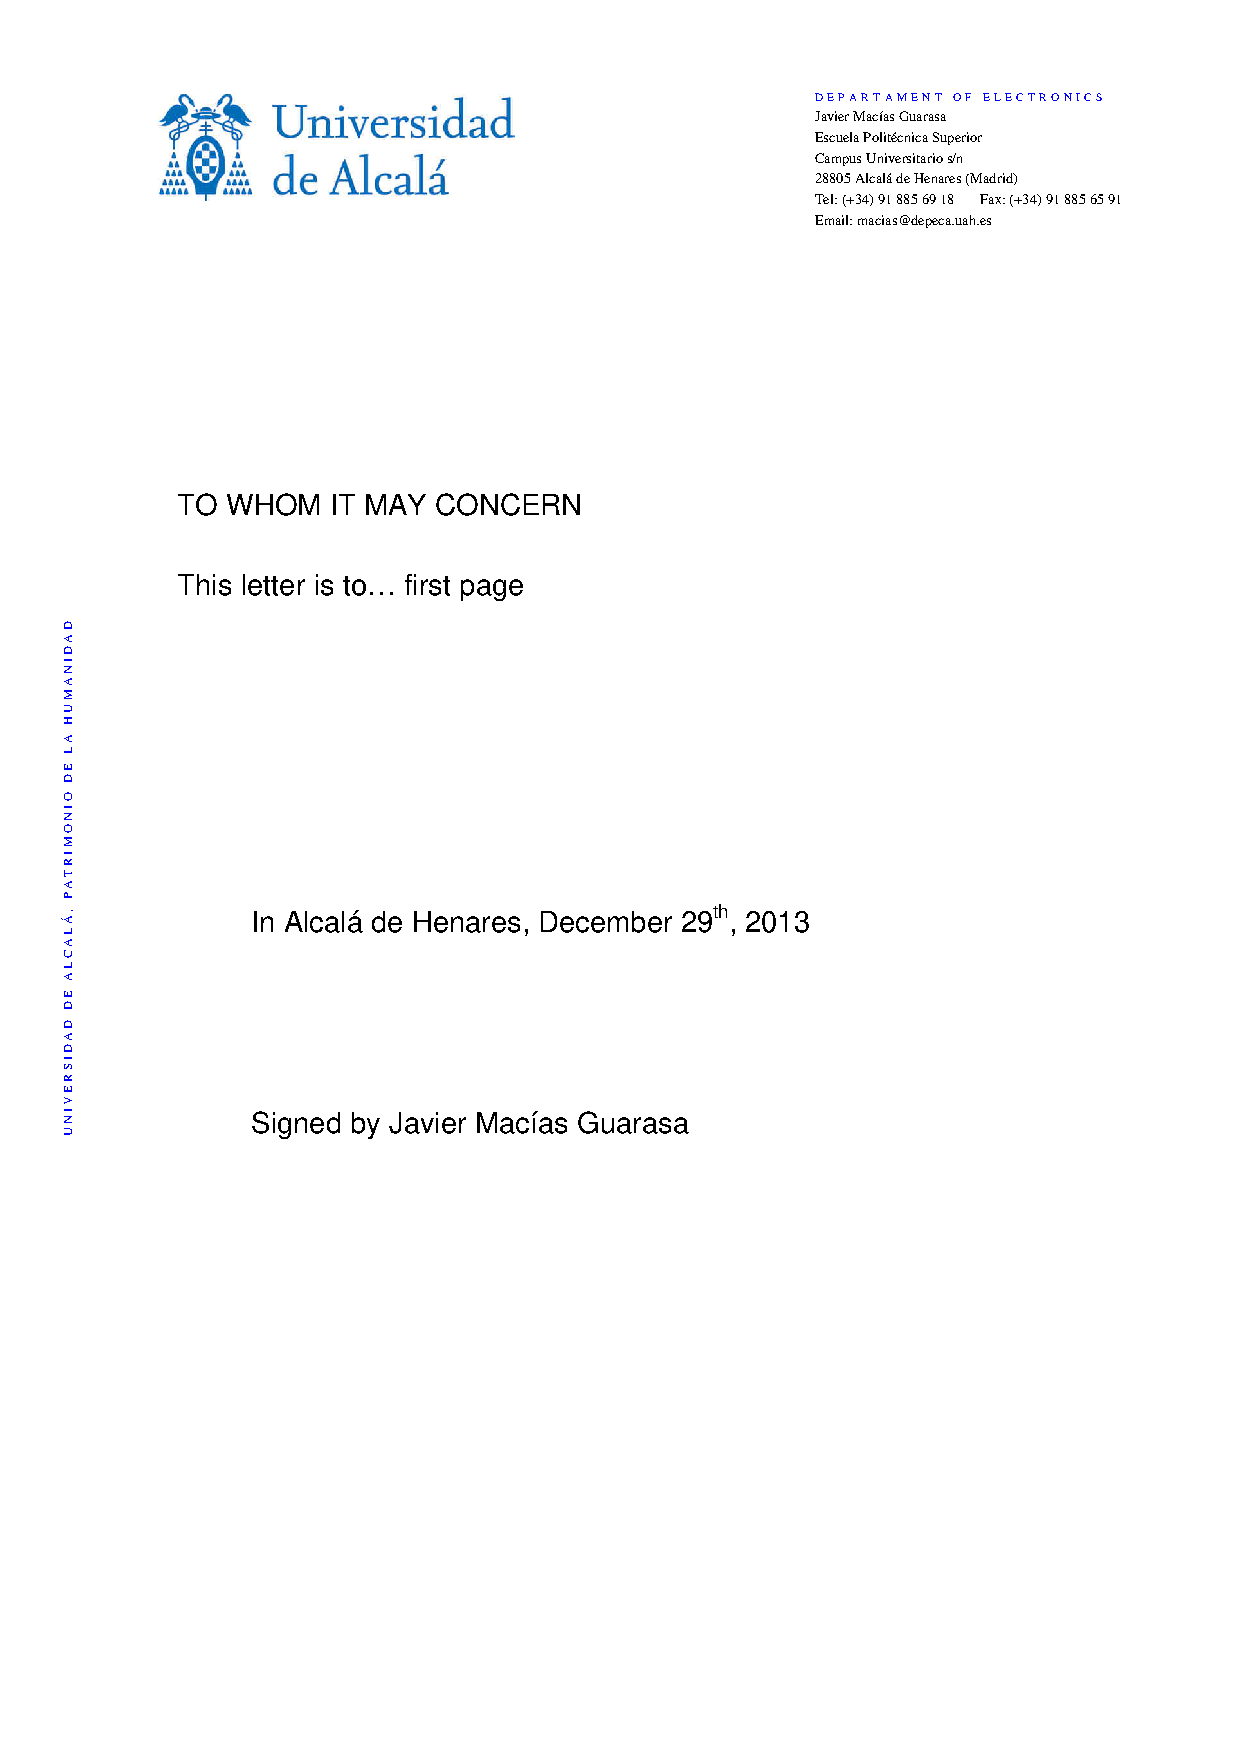
\includepdf[pages=-]{letters/sampleLetter-pages.pdf}   % include all pages of
%                                                 % pdf file
\clearemptydoublepage % You need to add this after including each pdf

%\includepdf[pages=-]{papeleo/vistoBuenoTutorTFM-MUSEA.pdf}   % for TFMs
%\clearemptydoublepage % You need to add this after including each pdf

% Dedication+ackowledgements (dedicatorias+agradecimientos)
%%%%%%%%%%%%%%%%%%%%%%%%%%%%%%%%%%%%%%%%%%%%%%%%%%%%%%%%%%%%%%%%%%%%%%%%%%% 
% 
% Generic template for TFC/TFM/TFG/Tesis
% 
% $Id: dedicatoria.tex,v 1.5 2015/06/05 00:10:35 macias Exp $
% 
% By:
% + Javier Macías-Guarasa. 
% Departamento de Electrónica
% Universidad de Alcalá
% + Roberto Barra-Chicote. 
% Departamento de Ingeniería Electrónica
% Universidad Politécnica de Madrid   
% 
% Based on original sources by Roberto Barra, Manuel Ocaña, Jesús Nuevo,
% Pedro Revenga, Fernando Herránz and Noelia Hernández. Thanks a lot to
% all of them, and to the many anonymous contributors found (thanks to
% google) that provided help in setting all this up.
% 
% See also the additionalContributors.txt file to check the name of
% additional contributors to this work.
% 
% If you think you can add pieces of relevant/useful examples,
% improvements, please contact us at (macias@depeca.uah.es)
% 
% You can freely use this template and please contribute with
% comments or suggestions!!!
% 
%%%%%%%%%%%%%%%%%%%%%%%%%%%%%%%%%%%%%%%%%%%%%%%%%%%%%%%%%%%%%%%%%%%%%%%%%%% 

% 
% This is also courtesy of Roberto Barra
% 
% To center text in a page:
% \topskip0pt
% \vspace*{\fill}
% text
% \vspace*{\fill}

\thispagestyle{empty}

\begin{flushright}

  \topskip0pt
  \vspace*{\fill}

  \textbf{A mi Madre, allá donde esté ...\ldots}\\

  \vspace{3cm}

  \emph{``En este vasto mundo \\
  	navegáis en pos de un sueño,  \\
  	surcando el ancho mar  \\
  	que se extiende frente a vosotros.  \\
  	El puerto de destino es el mañana  \\
  	cada día más incierto.  \\
  	Encontrad el camino,  \\
  	cumplid vuestros sueños,  \\
  	estáis todos en el mismo barco  \\
  	y vuestra bandera es la libertad”  \\
  	Espero que te guste Mamá, allá donde estés …''}\\ 
    Opening 3 de One Piece. \\
    Autor: The Babystars

\end{flushright}  

\vspace{4cm}
\vspace*{\fill}

% \clearemptydoublepage



%%% Local Variables:
%%% TeX-master: "../book"
%%% End:
            % EDIT this file or
                                              % comment it out
                                              
%%%%%%%%%%%%%%%%%%%%%%%%%%%%%%%%%%%%%%%%%%%%%%%%%%%%%%%%%%%%%%%%%%%%%%%%%%%
%
% Generic template for TFC/TFM/TFG/Tesis
%
% $Id: agradecimientos.tex,v 1.7 2015/06/05 00:10:31 macias Exp $
%
% By:
%  + Javier Macías-Guarasa. 
%    Departamento de Electrónica
%    Universidad de Alcalá
%  + Roberto Barra-Chicote. 
%    Departamento de Ingeniería Electrónica
%    Universidad Politécnica de Madrid   
% 
% Based on original sources by Roberto Barra, Manuel Ocaña, Jesús Nuevo,
% Pedro Revenga, Fernando Herránz and Noelia Hernández. Thanks a lot to
% all of them, and to the many anonymous contributors found (thanks to
% google) that provided help in setting all this up.
%
% See also the additionalContributors.txt file to check the name of
% additional contributors to this work.
%
% If you think you can add pieces of relevant/useful examples,
% improvements, please contact us at (macias@depeca.uah.es)
%
% You can freely use this template and please contribute with
% comments or suggestions!!!
%
%%%%%%%%%%%%%%%%%%%%%%%%%%%%%%%%%%%%%%%%%%%%%%%%%%%%%%%%%%%%%%%%%%%%%%%%%%%

% Use this if you don't like the fancy style
\thispagestyle{empty}

\ifthenelse{\equal{\myLanguage}{english}}
{
  \chapter*{Acknowledgements}
  \label{cha:acknowledgements}
  \markboth{Acknowledgements}{Acknowledgements}
  \addcontentsline{toc}{chapter}{Acknowledgements}
}
{
  \chapter*{Agradecimientos}
  \label{cha:agradecimientos}
  \markboth{Agradecimientos}{Agradecimientos}
  \addcontentsline{toc}{chapter}{Agradecimientos}
}

% ``Más vale un minuto de ilusión que mil horas de
% razonamiento''... (cortesía de Roberto Barra)


Esta Tesis Doctoral supone el culmen a cuatro años (Abril 2019 - Abril 2023) realmente duros, cargado de emociones, triunfos, pandemias, estafas y tropiezos, todo a partes iguales. Este es probablemente (aunque como diría Sean Connery interpretando a James Bond en 1983, \textit{Never Say Never Again}) mi último gran documento individual, académicamente hablando. Durante mi etapa universitaria (2013 hasta el momento, 2023) he tenido ciertos momentos puntuales en los que he sentido un salto cualitativo como profesional: El primero fue en el segundo cuatrimestre de segundo de carrera, cuando las cosas se pusieron tensas con Control II e Informática Industrial. Vaya sudores. El segundo probablemente fue con el fallecimiento de mi madre durante mi ERASMUS+ en Irlanda. Duros y oscuros momentos, alejado de mis seres queridos. El tercer momento llega en segundo de máster, durante mi querido ERASMUS+ en Finlandia, donde compagino una estancia preciosa en Tampere con el máster y un pre-inicio de doctorado. Me equivoqué al empezar tan pronto con la beca, "queriendo cobrar" cuanto antes, en vez de terminar tranquilamente el TFM y plantear tranquilamente la tesis, pero eso no lo sabría hasta tiempo después. Por último, toda la tesis han sido sube y bajas, con mala planificación por mi parte, momentos puntuales donde me equivoqué rotundamente al no estudiar PyTorch tras el WAF 2018 tras la sugerencia de mi tutor, el no enfocarme en técnica individual hasta bien entrado el doctorado, no querer hacer nada hasta que no tuviese la teoría perfectamente asimilada, tener demasiado respeto a la Inteligencia Artificial y escurrir el bulto de mi tesis en un compañero mientras yo me dedicaba a integrar y corregir los bugs del grupo que para mí era lo fácil. Mal. Todo mal. Pero todo cambió tras mi segunda estancia, en Estados Unidos, cuando tras llorar por no entender el camino a seguir, decidí crear mi propio camino, con paciencia, fé y práctica y error compaginado con lectura de artículos, para mejorar mi confianza y autoestima, y finalmente logré empezar a entender lo que era el Deep Learning. Gracias a todos mis errores, desventuras y discusiones, a día de hoy, excepto momentos inevitables, me encuentro con muchísima capacidad en atacar prácticamente cualquier problema. Cada año, desde hace ya varios, mi primera publicación en Instagram viene seguida de la frase "Trabaja duro en silencio y deja que tu éxito haga todo el ruido". Filosofía Kaizen, de mejora y aprendizaje continuo, para así cada día entender el mundo un poquito mejor. Si toda la dedicación y estudio que he depositado en este trabajo sirven para algo en mi futuro, sé que todo el esfuerzo habrá merecido la pena.

Después de este particular monólogo, a lo cual soy muy propenso y de lo cual mis amigos y compañeros no cesan en su empeño de recordármelo, debo, como no puede ser de otra manera, dar paso a los agradecimientos.


En primer lugar, me gustaría agradecer a mis profesores del grupo RobeSafe, especialmente a mis tutores Luis Miguel Bergasa Pascual y Rafael Barea Navarro, por ofrecerme estar en el grupo (así como aguantarme) durante estos todos estos años e intentar que tuviésemos el mejor experimental setup en el laboratorio, aunque no fuese siempre sencillo. Sin dudas considero realmente interesante la temática propuesta en esta tesis doctoral, predicción de agentes en conducción autónoma, ya que entra en el plano filosófico sobre cómo razonar el futuro de los objetos y cómo podría afectar a la capacidad ejecutiva del agente que tenga que tomar una decisión. Mi mente hace tiempo que cambió y me fijo siempre que conduzco de todo lo que intento reproducir con mis estudios. Habrá que seguir esta tendencia muy de cerca en los próximos años.

A mis tutores en las estancias de doctorado, Christoph Stiller y Eduardo Molinos en el KIT y Wei Zhan y Masayoshi Tomizuka en Berkeley. Se suele decir que unas veces se gana y otras se aprende, y yo en estas estancias aprendí demasiado.

A mis compañeros, mejor dicho, amigos, de laboratorio: Javier Araluce, Rodrigo, Felipe (chavalín), Santiago, Miguel Antunes,
antiguos compañeros como Javier del Egido, Óscar, Alejandro, Eduardo, Roberto y Pablo, y a nuevos becarios como Fabio, Navil y Pablo. Gracias de corazón por estar ahí, en nuestras charlas sobre tecnología, empleos, el camino correcto a seguir y la vida en general.

A mis amigos de la universidad, especialmente a Rocío, Juan Carlos, Esther, Sergio, Pablo, Rubén y Adrián Rocandio. Aún me acuerdo de cuando empezamos con la carrera y como ahora la vida nos va perfilando poco a poco a cada uno. Os deseo lo mejor en vuestro futuro.

A mis buenos amigos Samuel y Adrián, con quien gran parte de mi vida he compartido. Con especial cariño guardo las interminables charlas sobre la vida y el futuro después de entrenar, de comer, de cenar, en el coche.

A mi familia, uno de los pilares de mi vida. A mi padre Juan Antonio y a mi madre Petra, que en paz descanse, les debo todo lo que soy y es por ello por lo que les estaré siempre agradecido. Querida madre, no se muere quien se va, sólo se muere el que se olvida, y tú nunca caerás en el olvido. A mi querida hermana-calili-chessmaster Silvia, con quien tantas regañinas he tenido, pero el cariño que nos tenemos las supera a todas. A mi perrita Nuka (a.k.a. dragón o Nuki-Nuki), cuyos paseos matutinos son probablemente el ingrediente secreto para la elaboración de esta tesis, dando rienda suelta a mi cabeza para imaginar nuevas
propuestas mientras miraba el cielo azul. 

Al resto de la familia, amigos y compañeros, gracias por todo.

Y, por último, la persona más importante de mi vida ahora mismo. Mi querida Marta, la persona más maravillosa y buena que conozco. Hemos compartido risas, lloros, besos y abrazos. Nunca me cansaré de repetirte lo suave que tienes la piel tras darte un beso en la mejilla y después hacerte de rabiar. Espero que esta situación esté dentro de un while cuya condición sea True.
"Te quiero más que ayer, pero menos que mañana. Hoy, y siempre"

Vamos a la lectura importante compañeros!

% Back to normal JIC. Use it if you set \pagestyle{myplain} above
%\pagestyle{fancy}

%%% Local Variables:
%%% TeX-master: "../book"
%%% End:  % EDIT this file or
                                              % comment it out

% If this is the case, include definitions of acronyms (it's
% included before resumen.tex and abstract.tex in case you want
% to use them here
%%%%%%%%%%%%%%%%%%%%%%%%%%%%%%%%%%%%%%%%%%%%%%%%%%%%%%%%%%%%%%%%%%%%%%%%%%%
%
% Generic template for TFC/TFM/TFG/Tesis
%
% $Id: defacronymsgl.tex,v 1.2 2015/06/05 00:10:31 macias Exp $
%
% By:
%  + Javier Macías-Guarasa. 
%    Departamento de Electrónica
%    Universidad de Alcalá
%  + Roberto Barra-Chicote. 
%    Departamento de Ingeniería Electrónica
%    Universidad Politécnica de Madrid   
% 
% Based on original sources by Roberto Barra, Manuel Ocaña, Jesús Nuevo,
% Pedro Revenga, Fernando Herránz and Noelia Hernández. Thanks a lot to
% all of them, and to the many anonymous contributors found (thanks to
% google) that provided help in setting all this up.
%
% See also the additionalContributors.txt file to check the name of
% additional contributors to this work.
%
% If you think you can add pieces of relevant/useful examples,
% improvements, please contact us at (macias@depeca.uah.es)
%
% You can freely use this template and please contribute with
% comments or suggestions!!!
%
%%%%%%%%%%%%%%%%%%%%%%%%%%%%%%%%%%%%%%%%%%%%%%%%%%%%%%%%%%%%%%%%%%%%%%%%%%%

% This file shows some examples for glossary terms

%%%%%%%%%%%%%%%%%%%%%%%%%%%%%%%%%%%%%%%%%%%%%%%%%%%%%%%%%%%%%%%%%%%%%%%%%%%
% BEGIN example of glossary terms definition
%
\newacronym{LSTM}{LSTM}{Long Short-Term Memory}
\newacronym{SOTA}{SOTA}{State-of-the-Art}
\newacronym{GAN}{GAN}{Generative Adversarial Network}
\newacronym{GNN}{GNN}{Graph Neural Network}
\newacronym{AI}{AI}{Artificial Intelligence}
\newacronym{ADE}{ADE}{Average Displacement Error}
\newacronym{FDE}{FDE}{Final Displacement Error}
\newacronym{AD}{AD}{Autonomous Driving}
\newacronym{ADS}{ADS}{Autonomous Driving Stack}
\newacronym{ITS}{ITS}{Intelligent Transportation Systems}
\newacronym{MP}{MP}{Motion Prediction}
\newacronym{BEV}{BEV}{Bird's Eye View}
\newacronym{DL}{DL}{Deep Learning}

% In the future version of texlive, we will be able to use longplural
% and shortplural. Right now we must use \newglossaryentry.

%
% END example of glossary terms definition
%%%%%%%%%%%%%%%%%%%%%%%%%%%%%%%%%%%%%%%%%%%%%%%%%%%%%%%%%%%%%%%%%%%%%%%%%%%


%%% Local Variables:
%%% TeX-master: "../book"
%%% End:
            % EDIT this file or
                                              % comment it out if you do
                                              % not use acronyms

% If this is the case, include definitions of acronyms (it's
% included before resumen.tex and abstract.tex in case you want
% to use them there
%%%%%%%%%%%%%%%%%%%%%%%%%%%%%%%%%%%%%%%%%%%%%%%%%%%%%%%%%%%%%%%%%%%%%%%%%%%
%
% Generic template for TFC/TFM/TFG/Tesis
%
% $Id: defsymbolsgl.tex,v 1.2 2015/06/05 00:10:37 macias Exp $
%
% By:
%  + Javier Macías-Guarasa. 
%    Departamento de Electrónica
%    Universidad de Alcalá
%  + Roberto Barra-Chicote. 
%    Departamento de Ingeniería Electrónica
%    Universidad Politécnica de Madrid   
% 
% Based on original sources by Roberto Barra, Manuel Ocaña, Jesús Nuevo,
% Pedro Revenga, Fernando Herránz and Noelia Hernández. Thanks a lot to
% all of them, and to the many anonymous contributors found (thanks to
% google) that provided help in setting all this up.
%
% See also the additionalContributors.txt file to check the name of
% additional contributors to this work.
%
% If you think you can add pieces of relevant/useful examples,
% improvements, please contact us at (macias@depeca.uah.es)
%
% You can freely use this template and please contribute with
% comments or suggestions!!!
%
%%%%%%%%%%%%%%%%%%%%%%%%%%%%%%%%%%%%%%%%%%%%%%%%%%%%%%%%%%%%%%%%%%%%%%%%%%%

% These ones for the symbols glossary

%%%%%%%%%%%%%%%%%%%%%%%%%%%%%%%%%%%%%%%%%%%%%%%%%%%%%%%%%%%%%%%%%%%%%%%%%%%
% BEGIN example of symbols definition
%
\newglossaryentry{ohm}{type=symbols,
        name={\ensuremath{\Omega}},
        symbol={\ensuremath{\Omega}}, 
        sort=ohm,
        description=unit of electrical resistance}

\newglossaryentry{angstrom}{type=symbols,
        name={\AA},
        symbol={\AA},
        sort=angstrom,
        description={non-SI unit of length}}

\newglossaryentry{xdet}{type=symbols,
        name={\ensuremath{x(t)}},
        symbol={\ensuremath{x(t)}},
        sort=xdet,
        description={Audio signal}}

\newglossaryentry{xidet}{type=symbols,
        name={\ensuremath{x_i(t)}},
        symbol={\ensuremath{x_i(t)}},
        sort=xidet,
        description={Audio signal captured at microphone $i$}}

\newglossaryentry{condindep}{type=symbols,
        name={\ensuremath{\ci}},
        symbol={\ensuremath{\ci}}, 
        sort=conditionalindependence,
        description=conditional independence}

%
% END example of symbols definition
%%%%%%%%%%%%%%%%%%%%%%%%%%%%%%%%%%%%%%%%%%%%%%%%%%%%%%%%%%%%%%%%%%%%%%%%%%%

%%% Local Variables:
%%% TeX-master: "../book"
%%% End:
              % EDIT this file or
                                              % comment it out if you do
                                              % not use acronyms

% Now include resumen and abstract
%%%%%%%%%%%%%%%%%%%%%%%%%%%%%%%%%%%%%%%%%%%%%%%%%%%%%%%%%%%%%%%%%%%%%%%%%%%
%
% Generic template for TFC/TFM/TFG/Tesis
%
% $Id: resumen.tex,v 1.9 2015/06/05 00:10:31 macias Exp $
%
% By:
%  + Javier Macías-Guarasa. 
%    Departamento de Electrónica
%    Universidad de Alcalá
%  + Roberto Barra-Chicote. 
%    Departamento de Ingeniería Electrónica
%    Universidad Politécnica de Madrid   
% 
% Based on original sources by Roberto Barra, Manuel Ocaña, Jesús Nuevo,
% Pedro Revenga, Fernando Herránz and Noelia Hernández. Thanks a lot to
% all of them, and to the many anonymous contributors found (thanks to
% google) that provided help in setting all this up.
%
% See also the additionalContributors.txt file to check the name of
% additional contributors to this work.
%
% If you think you can add pieces of relevant/useful examples,
% improvements, please contact us at (macias@depeca.uah.es)
%
% You can freely use this template and please contribute with
% comments or suggestions!!!
%
%%%%%%%%%%%%%%%%%%%%%%%%%%%%%%%%%%%%%%%%%%%%%%%%%%%%%%%%%%%%%%%%%%%%%%%%%%%

\chapter*{Resumen}
\label{cha:resumen}
\markboth{Resumen}{Resumen}

\addcontentsline{toc}{chapter}{Resumen}

La conducción autónoma es considerada como una de los más grandes retos tecnológicos actuales. Cuando los coches autónomos conquisten nuestras carreteras, los accidentes se reducirán notablemente, hasta casi desaparecer, ya que la tecnología estará testada y no incumplirá las normas de conducción, entre otros beneficios sociales y económicos.

Uno de los aspectos más críticos a la hora de desarrollar un vehículo autónomo es percibir y entender la escena que le rodea. Esta tarea debe ser tan precisa y eficiente como sea posible para posteriormente predecir el futuro de esta misma y ayudar a la toma de decisiones. De esta forma, las acciones tomadas por el vehículo garantizarán tanto la seguridad del vehículo en sí mismo y sus ocupantes, como la de los obstáculos circundantes, tales como viandantes, otros vehículos o infraestructura de la carretera.

En ese sentido, esta tesis doctoral se centra en el estudio y desarrollo de distintas técnicas predictivas para el entendimiento de la escena en el contexto de la conducción autónoma. Durante la tesis, se observa una incorporación progresiva de técnicas de aprendizaje profundo en los distintos algoritmos propuestos para mejorar el razonamiento sobre qué está ocurriendo en el escenario de tráfico así como modelar las complejas interacciones entre la información social (distintos participantes o agentes del escenario, tales como vehículos, ciclistas o peatones) y física (es decir, la información geométrica, semántica y topológica del mapa de alta definición) presente en la escena. 

La capa de percepción de un vehículo autónomo se divide modularmente en tres etapas: Detección, Monitorización y Predicción. Para iniciar el estudio de las etapas de monitorización y predicción, se propone un algoritmo de \textit{Multi-Object Tracking} basado en técnicas clásicas de estimación de movimiento y asociación validado en el dataset KITTI, el cual tiene métricas del estado del arte. Por otra parte, se propone el uso de un filtro inteligente basado en información contextual de mapa, cuyo objetivo es monitorizar los agentes más relevantes de la escena en el tiempo, representando estos agentes filtrados la entrada preliminar para realizar predicciones unimodales basadas en un modelo cinemático. Para validar esta propuesta de filtro inteligente se usa CARLA, uno de los simuladores hiperrealistas para conducción autónoma más prometedores en la actualidad, comprobando cómo al usar información contextual de mapa se puede reducir notablemente el tiempo de inferencia de \textit{tracking} y predicción prestando atención a los agentes realmente relevantes del escenario de tráfico.

Tras observar las limitaciones de un modelo de predicción basado en cinemática para la predicción a largo plazo de un agente, los distintos algoritmos de la tesis se centran en el módulo de predicción, usando los datasets Argoverse 1 y Argoverse 2, donde se asume que los agentes proporcionados en cada escenario de tráfico ya están monitorizados durante un cierto número de observaciones. 

En primer lugar, se introduce un modelo basado en redes neuronales recurrentes (particularmente redes LSTM, \textit{Long-Short Term Memory}) y mecanismo de atención para codificar las trayectorias pasadas de los agentes, y una representación simplificada del mapa en forma de posiciones finales potenciales en la carretera para calcular las trayectorias futuras unimodales, todo envuelto en un marco GAN (\textit{Generative Adversarial Network}), obteniendo métricas similares al estado del arte en el caso unimodal.

Una vez validado el modelo anterior en Argoverse 1, se proponen distintos modelos (sólo social, incorporando mapa, y una mejora final basada en \textit{Transformer encoder} y redes convolucionales 1D) base precisos y eficientes basados en el modelo de predicción anterior, introduciendo el uso de las redes gráficas (particularmente GCN, \textit{Graph Convolutional Network}) para codificar de una forma potente las interacciones de los agentes y el preprocesamiento de trayectorias preliminares a partir de mapa con un método heurístico, para posteriormente predecir distintas trayectorias futuras en este caso multimodales, es decir, cubriendo distintos posibles futuros para el agente de interés. Los modelos base propuestos obtienen métricas de regresión del estado del arte tanto en el caso multimodal como unimodal manteniendo un claro compromiso de eficiencia con respecto a otras propuestas.

El modelo final de la tesis, inspirado en los modelos anteriores y validado en el más reciente dataset para algoritmos de predicción en conducción autónoma (Argoverse 2), introduciendo la información topológica y semántica de los carriles futuros preliminares con el método heurístico antes mencionado, codificación de mapa basada en aprendizaje profundo con redes GCN, ciclo de fusión de características físicas y sociales, estimación de posiciones finales en la carretera con aprendizaje profundo y agregación de su entorno circundante, y finalmente módulo de refinado para mejorar la calidad de las predicciones multimodales finales de un modo elegante y eficiente. Comparado con el estado del arte, nuestro método logra métricas de predicción a la par con los métodos mejor posicionados en el Leaderboard de Argoverse 2, reduciendo de forma notable el número de parámetros y operaciones de coma flotante por segundo.

Finalmente, este modelo final es validado en simulación en distintas aplicaciones de conducción autónoma, como la toma de decisiones en el simulador SMARTS o el estudio de adaptación de dominio en el simulador hiperrealista CARLA con otras capas del vehículo como paso preliminar a su implementación en un vehículo autónomo real.

\textbf{Palabras clave:} \myThesisKeywords.

%%% Local Variables:
%%% TeX-master: "../book"
%%% End:


                  % EDIT this file
%%%%%%%%%%%%%%%%%%%%%%%%%%%%%%%%%%%%%%%%%%%%%%%%%%%%%%%%%%%%%%%%%%%%%%%%%%%
%
% Generic template for TFC/TFM/TFG/Tesis
%
% $Id: abstract.tex,v 1.9 2015/06/05 00:10:31 macias Exp $
%
% By:
%  + Javier Macías-Guarasa. 
%    Departamento de Electrónica
%    Universidad de Alcalá
%  + Roberto Barra-Chicote. 
%    Departamento de Ingeniería Electrónica
%    Universidad Politécnica de Madrid   
% 
% Based on original sources by Roberto Barra, Manuel Ocaña, Jesús Nuevo,
% Pedro Revenga, Fernando Herránz and Noelia Hernández. Thanks a lot to
% all of them, and to the many anonymous contributors found (thanks to
% google) that provided help in setting all this up.
%
% See also the additionalContributors.txt file to check the name of
% additional contributors to this work.
%
% If you think you can add pieces of relevant/useful examples,
% improvements, please contact us at (macias@depeca.uah.es)
%
% You can freely use this template and please contribute with
% comments or suggestions!!!
%
%%%%%%%%%%%%%%%%%%%%%%%%%%%%%%%%%%%%%%%%%%%%%%%%%%%%%%%%%%%%%%%%%%%%%%%%%%%

\chapter*{Abstract}
\label{cha:abstract}

\addcontentsline{toc}{chapter}{Abstract}

Autonomous driving is considered one of the greatest technological challenges of the present time. When autonomous cars take over our roads, accidents will be significantly reduced, to the point of almost disappearing, as the technology will be thoroughly tested and will not violate driving regulations, such as speeding, dangerous overtaking, or driver distractions, among other factors.

One of the most critical aspects in developing an autonomous vehicle is perceiving and understanding the surrounding scene as precisely and efficiently as possible in order to predict its future and assist in decision-making. Thus, the actions taken by the vehicle or driver, in the case of partially autonomous driving, must ensure the safety of the vehicle itself, its occupants, and the surrounding obstacles, such as pedestrians, other vehicles, or road infrastructure.

In this regard, this doctoral thesis focuses on the study and development of various predictive techniques for scene understanding in the context of autonomous driving, progressively incorporating deep learning into the proposed algorithms to improve reasoning about what is happening in the traffic scenario and model the complex interactions among different participants or agents in the scene (such as vehicles, cyclists, or pedestrians), as well as the geometric, semantic, and topological information from the high-definition map present in the scene.

Firstly, an algorithm based on classical motion estimation and association techniques is proposed, along with an intelligent filter based on contextual map information. Its objective is to monitor the different agents over time, providing a preliminary input for making predictions based on a kinematic model. This model investigates how using contextual map information can significantly reduce inference time by focusing on the truly relevant agents in the traffic scenario.

Secondly, a model based on recurrent neural networks and attention mechanism is introduced to encode the past trajectories of the agents, along with a simplified representation of the map in the form of potential final positions on the road. This model calculates uni-modal future trajectories, all within a generative adversarial network framework.

Thirdly, different accurate and efficient baselines are proposed based on the aforementioned prediction model. These models introduce the use graph neural networks to powerfully encode agent interactions and preprocess preliminary trajectories from the map using a heuristic method. They then predict various multi-modal future trajectories, covering different possible futures for the target agent.

Taking these previous points into consideration, the final model of the thesis improves upon the previous ones by incorporating enhancements in the heuristic method, including topological and semantic information of interest about lanes, deep learning-based map encoding, fusion of physical and social features, deep learning-based estimation of final positions on the road, aggregation of the surrounding environment, and refinement of predictions to enhance the quality of the final multi-modal predictions in an elegant and efficient manner.

Finally, this final model is validated in various autonomous driving applications, such as decision-making or holistic integration in a hyper-realistic simulator with other vehicle layers, as a preliminary step towards its implementation in an actual autonomous vehicle.

\textbf{Keywords:} \myThesisKeywordsEnglish.

%%% Local Variables:
%%% TeX-master: "../book"
%%% End:


                 % EDIT this file

% Just for TFGs/PFCs at UAH, I do nothing and leave to the author the
% inclusion of the file
%%%%%%%%%%%%%%%%%%%%%%%%%%%%%%%%%%%%%%%%%%%%%%%%%%%%%%%%%%%%%%%%%%%%%%%%%%%%
%
% Generic template for TFC/TFM/TFG/Tesis
%
% $Id: resumen-extendido.tex,v 1.6 2015/06/05 00:10:31 macias Exp $
%
% By:
%  + Javier Macías-Guarasa. 
%    Departamento de Electrónica
%    Universidad de Alcalá
%  + Roberto Barra-Chicote. 
%    Departamento de Ingeniería Electrónica
%    Universidad Politécnica de Madrid   
% 
% Based on original sources by Roberto Barra, Manuel Ocaña, Jesús Nuevo,
% Pedro Revenga, Fernando Herránz and Noelia Hernández. Thanks a lot to
% all of them, and to the many anonymous contributors found (thanks to
% google) that provided help in setting all this up.
%
% See also the additionalContributors.txt file to check the name of
% additional contributors to this work.
%
% If you think you can add pieces of relevant/useful examples,
% improvements, please contact us at (macias@depeca.uah.es)
%
% You can freely use this template and please contribute with
% comments or suggestions!!!
%
%%%%%%%%%%%%%%%%%%%%%%%%%%%%%%%%%%%%%%%%%%%%%%%%%%%%%%%%%%%%%%%%%%%%%%%%%%%

\ifthenelse{\equal{\myLanguage}{english}}
{
\chapter*{Extended Abstract}
\label{cha:resumen-extendido}
\markboth{Extended Abstract}{Extended Abstract}

\addcontentsline{toc}{chapter}{Extended Abstract}
}
{
\chapter*{Resumen extendido}
\label{cha:resumen-extendido}
\markboth{Resumen extendido}{Resumen extendido}

\addcontentsline{toc}{chapter}{Resumen extendido}
}

Con un máximo de cuatro o cinco páginas. Se supone que sólo está
definido como obligatorio para los TFGs y PFCs de UAH.

%%% Local Variables:
%%% TeX-master: "../book"
%%% End:


       % EDIT this file

% Now include toc and list of figures+tables
%%%%%%%%%%%%%%%%%%%%%%%%%%%%%%%%%%%%%%%%%%%%%%%%%%%%%%%%%%%%%%%%%%%%%%%%%%%
%
% Generic template for TFC/TFM/TFG/Tesis
%
% $Id: toc+lof+lot.tex,v 1.9 2015/06/05 00:10:34 macias Exp $
%
% By:
%  + Javier Macías-Guarasa. 
%    Departamento de Electrónica
%    Universidad de Alcalá
%  + Roberto Barra-Chicote. 
%    Departamento de Ingeniería Electrónica
%    Universidad Politécnica de Madrid   
% 
% Based on original sources by Roberto Barra, Manuel Ocaña, Jesús Nuevo,
% Pedro Revenga, Fernando Herránz and Noelia Hernández. Thanks a lot to
% all of them, and to the many anonymous contributors found (thanks to
% google) that provided help in setting all this up.
%
% See also the additionalContributors.txt file to check the name of
% additional contributors to this work.
%
% If you think you can add pieces of relevant/useful examples,
% improvements, please contact us at (macias@depeca.uah.es)
%
% You can freely use this template and please contribute with
% comments or suggestions!!!
%
%%%%%%%%%%%%%%%%%%%%%%%%%%%%%%%%%%%%%%%%%%%%%%%%%%%%%%%%%%%%%%%%%%%%%%%%%%%

\hypersetup{linkcolor=\mytoclinkcolor}
\tableofcontents

\hypersetup{linkcolor=\myloflinkcolor}
\listoffigures
                          
\hypersetup{linkcolor=\mylotlinkcolor}
\listoftables

\hypersetup{linkcolor=\mylinkcolor}

%%% Local Variables:
%%% TeX-master: "../book"
%%% End:
                 % DO NOT TOUCH THIS LINE!

% If you want to include additional listings, you can use the float
% package. As an example, I include here the listing of source code
% snippets and algorithms (you have some examples in
% appendix/manual.tex)
%%%%%%%%%%%%%%%%%%%%%%%%%%%%%%%%%%%%%%%%%%%%%%%%%%%%%%%%%%%%%%%%%%%%%%%%%%%
%
% Generic template for TFC/TFM/TFG/Tesis
%
% $Id: extralistings.tex,v 1.5 2015/06/05 00:10:34 macias Exp $
%
% By:
%  + Javier Macías-Guarasa. 
%    Departamento de Electrónica
%    Universidad de Alcalá
%  + Roberto Barra-Chicote. 
%    Departamento de Ingeniería Electrónica
%    Universidad Politécnica de Madrid   
% 
% Based on original sources by Roberto Barra, Manuel Ocaña, Jesús Nuevo,
% Pedro Revenga, Fernando Herránz and Noelia Hernández. Thanks a lot to
% all of them, and to the many anonymous contributors found (thanks to
% google) that provided help in setting all this up.
%
% See also the additionalContributors.txt file to check the name of
% additional contributors to this work.
%
% If you think you can add pieces of relevant/useful examples,
% improvements, please contact us at (macias@depeca.uah.es)
%
% You can freely use this template and please contribute with
% comments or suggestions!!!
%
%%%%%%%%%%%%%%%%%%%%%%%%%%%%%%%%%%%%%%%%%%%%%%%%%%%%%%%%%%%%%%%%%%%%%%%%%%%

\begin{comment}
% Include the list of source code listings (if this is the case)
\hypersetup{linkcolor=\myothertoclinkcolor}
\ifthenelse{\equal{\myLanguage}{english}}
{
	\listof{codefloat}{List of Source Code}
	\addcontentsline{toc}{chapter}{List of Source Code}
}
{
	\listof{codefloat}{Índice de listados de código fuente}    
	\addcontentsline{toc}{chapter}{Índice de listados de código fuente}
}
\end{comment}
\begin{comment}
\ifthenelse{\equal{\myLanguage}{english}}
{
\renewcommand*{\algorithmcfname}{Algorithm}
\renewcommand{\listofalgorithms}{\begingroup
  \tocfile{List of Algorithms}{loa}
  \endgroup}
% \makeatletter
% \let\l@algorithm\l@figure
% \makeatother

}
\end{comment}
{
%\SetAlgorithmName{Algoritmo}{algoritmo}{Índice de algoritmos}
\renewcommand*{\algorithmcfname}{Algoritmo}
\renewcommand{\listofalgorithms}{\begingroup
   \tocfile{Índice de algoritmos}{loa}
   \endgroup}
 % \makeatletter
 % \let\l@algorithm\l@figure
 % \makeatother
}

\listofalgorithms

\hypersetup{linkcolor=\mylinkcolor}


%%% Local Variables:
%%% TeX-master: "../book"
%%% End:
               % Edit this file or
                                              % comment it out

% Now include list of acronyms and options (if this is the case)
%%%%%%%%%%%%%%%%%%%%%%%%%%%%%%%%%%%%%%%%%%%%%%%%%%%%%%%%%%%%%%%%%%%%%%%%%%%
%
% Generic template for TFC/TFM/TFG/Tesis
%
% $Id: acronymsgl.tex,v 1.8 2015/06/05 00:10:31 macias Exp $
%
% By:
%  + Javier Macías-Guarasa. 
%    Departamento de Electrónica
%    Universidad de Alcalá
%  + Roberto Barra-Chicote. 
%    Departamento de Ingeniería Electrónica
%    Universidad Politécnica de Madrid   
% 
% Based on original sources by Roberto Barra, Manuel Ocaña, Jesús Nuevo,
% Pedro Revenga, Fernando Herránz and Noelia Hernández. Thanks a lot to
% all of them, and to the many anonymous contributors found (thanks to
% google) that provided help in setting all this up.
%
% See also the additionalContributors.txt file to check the name of
% additional contributors to this work.
%
% If you think you can add pieces of relevant/useful examples,
% improvements, please contact us at (macias@depeca.uah.es)
%
% You can freely use this template and please contribute with
% comments or suggestions!!!
%
%%%%%%%%%%%%%%%%%%%%%%%%%%%%%%%%%%%%%%%%%%%%%%%%%%%%%%%%%%%%%%%%%%%%%%%%%%%

% You can change the way the entries appear the first time they are
% used. I've used italics by default. I found a problem if using this:
% LaTeX adds an extra space after the acronym, so I'm commenting it out
% (if you find a solution, please let me know)
%\defglsdisplayfirst[\acronymtype]{\textit{#1}} % EDIT this if required

% This may lead to problems... I don't know how to fix it in case the
% column for acronym is wider than 0.3\linewidth
\setlength{\glsdescwidth}{0.7\linewidth}       % EDIT this if required

% Set language specific definitions...
\ifthenelse{\equal{\myLanguage}{english}}
{
\printglossary[type=\acronymtype,style=super,nonumberlist=true,title=List of Acronyms,toctitle=List of Acronyms]
\addcontentsline{toc}{chapter}{List of Acronyms}
}
{
\printglossary[type=\acronymtype,style=super,nonumberlist=true,title=Lista de acrónimos,toctitle=Lista de acrónimos]
\addcontentsline{toc}{chapter}{Lista de acrónimos}
}


%%% Local Variables:
%%% TeX-master: "../book"
%%% End:


               % EDIT this file or
                                              % comment it out if you do
                                              % not use acronyms

%
% END within-document configuration, frontpage and cover pages generation
%%%%%%%%%%%%%%%%%%%%%%%%%%%%%%%%%%%%%%%%%%%%%%%%%%%%%%%%%%%%%%%%%%%%%%%%%%%

%%%%%%%%%%%%%%%%%%%%%%%%%%%%%%%%%%%%%%%%%%%%%%%%%%%%%%%%%%%%%%%%%%%%%%%%%%%
% Now start text and numbering for mainmatter (chapter+appendices)
%%%%%%%%%%%%%%%%%%%%%%%%%%%%%%%%%%%%%%%%%%%%%%%%%%%%%%%%%%%%%%%%%%%%%%%%%%%
\mainmatter                                       % DO NOT TOUCH THIS LINE!
\deactivatetilden                                 % DO NOT TOUCH THIS LINE!

%%%%%%%%%%%%%%%%%%%%%%%%%%%%%%%%%%%%%%%%%%%%%%%%%%%%%%%%%%%%%%%%%%%%%%%%%%%
%%%%%%%%%%%%%%%%%%%%%%%%%%%%%%%%%%%%%%%%%%%%%%%%%%%%%%%%%%%%%%%%%%%%%%%%%%%
%%%%%%%%%%%%%%%%%%%%%%%%%%%%%%%%%%%%%%%%%%%%%%%%%%%%%%%%%%%%%%%%%%%%%%%%%%%
%%%%%%%%%%%%%%%%%%%%%%%%%%%%%%%%%%%%%%%%%%%%%%%%%%%%%%%%%%%%%%%%%%%%%%%%%%%
%%%%%%%%%%%%%%%%%%%%%%%%%%%%%%%%%%%%%%%%%%%%%%%%%%%%%%%%%%%%%%%%%%%%%%%%%%%
%%%%%%%%%%%%%%%%%%%%%%%%%%%%%%%%%%%%%%%%%%%%%%%%%%%%%%%%%%%%%%%%%%%%%%%%%%%
%%%%%%%%%%%%%%%%%%%%%%%%%%%%%%%%%%%%%%%%%%%%%%%%%%%%%%%%%%%%%%%%%%%%%%%%%%%
% BEGIN Normal chapters. Edit/modify all within this section
%
% I don't recommend it, but if you want to define "parts", use this...
% BEWARE: I didn't write the english dependent code
%\part*{Memoria}
%\label{part:memoria}

%%%%%%%%%%%%%%%%%%%%%%%%%%%%%%%%%%%%%%%%%%%%%%%%%%%%%%%%%%%%%%%%%%%%%%%%%%% 
% 
% Generic template for TFC/TFM/TFG/Tesis
% 
% By:
% + Javier Macías-Guarasa. 
% Departamento de Electrónica
% Universidad de Alcalá
% + Roberto Barra-Chicote. 
% Departamento de Ingeniería Electrónica
% Universidad Politécnica de Madrid   
% 
% Based on original sources by Roberto Barra, Manuel Ocaña, Jesús Nuevo,
% Pedro Revenga, Fernando Herránz and Noelia Hernández. Thanks a lot to
% all of them, and to the many anonymous contributors found (thanks to
% google) that provided help in setting all this up.
% 
% See also the additionalContributors.txt file to check the name of
% additional contributors to this work.
% 
% If you think you can add pieces of relevant/useful examples,
% improvements, please contact us at (macias@depeca.uah.es)
% 
% You can freely use this template and please contribute with
% comments or suggestions!!!
% 
%%%%%%%%%%%%%%%%%%%%%%%%%%%%%%%%%%%%%%%%%%%%%%%%%%%%%%%%%%%%%%%%%%%%%%%%%%% 

\chapter{Introduction}
\label{cha:introduction}

\begin{FraseCelebre}
  \begin{Frase}
    Aaay, el oro, la fama, el poder.  \\
    Todo lo tuvo el hombre que en su día se autoproclamó  \\
    el rey de los piratas, ¡GOLD ROGER!  \\
    Mas sus últimas palabras no fueron muy afortunadas:  \\
    "¿¡MI TESORO!? Lo dejé todo allí, buscadlo si queréis,  \\
    ojalá se le atragante al rufián que lo encuentre.
  \end{Frase}
  \begin{Fuente}
    Opening 1 de One Piece: "We are" \\
    Autor original: Hiroshi Kitadani
  \end{Fuente}
\end{FraseCelebre}

\section{Motivation}
\label{sec:1_motivation}

\ac{AD} have held the attention of technology enthusiasts and futurists for some time as evidenced by the continuous research and development in \ac{ITS} over the past decades, being one of the emerging technologies of the \textit{Fourth Industrial Revolution}, and particularly of the Industry 4.0. \\

The concept \textit{Fourth Industrial Revolution} or Industry 4.0  was first introduced by Klaus Schwab , CEO (Chief Executive Officer) of the World Economic Forum, in a 2015 article in Foreign Affairs (American magazine of international relations and United States foreign policy). A technological revolution can be defined as a period in which one or more technologies are replaced by other kinds of technologies in a short amount of time. Hence, it is an era of accelerated technological progress featured by Researching, Development and Innovation whose rapid application and diffusion cause an abrupt change in society. In particular, the \textit{Fourth Industrial Revolution} conceptualizes rapid change to industries, technology, processes and societal patterns in the 21st century due to increasing inter-connectivity and smart automation. This industrial revolution focuses on operational efficiency, being the following four themes which summarize it: \\

\begin{itemize}
	\item Decentralized decisions: Ability of cyber physical systems to make decisions on their own and to perform their tasks as autonomously as possible.
	\item Information transparency: Provide operators with comprehensive information to make decisions. Inter-connectivity allows operators to gather large amounts of information and data from all points in the manufacturing process in order to identify key areas or aspects that can benefit from improvement to enhance functionality.
	\item Technical assistance: Ability to assist humans with unsafe or difficult tasks and technological facility of systems to help humans in problem-solving and decision-making.
	\item Interconnection: Ability of machines, sensors, devices and people to communicate and conect with each other via the Internet of Things (IoT) or the Internet of People (IoP).
\end{itemize}

Based on the aforementioned principles, this revolution is expected to be marked by breakthroughs in emerging technologies in fields such as nanotechnology, quantum computing, 3D printing, Internet of Things (IoT), fifth-generation wireless technologies (5G), Robotics, Computer Vision (CV), \ac{AI} or the scope of this PhD thesis, \acp{ADS}. The sum of all these advances are resulting in machines that can potentially see, hear and what is more important, think, moving more deftly than humans. \\

An \ac{ADS}, also referred in the literature as Intelligent Vehicle (IV), driverless car or autonomous car, is a vehicle tan can sense its surrounding and moving safely with little or even no human input. These \acp{ADS} must combine a variety of sensors to understand the traffic scenario, like RADAR (RAdio Detection A Ranging), LiDAR (Light Detection and Ranging), cameras, Inertial Measurement Unit (IMU), wheel odometry, GNSS (Global Navigation Satellite System) or ultrasonic sensors, and detect, track and predict (which is the main purpose of this thesis) the most relevant obstacles around the ego-vehicle. Then, advanced control and planning systems process this sensory information in combination with a predefined global route to calculate the corresponding control commands to drive throughout the environment, ensuring a safe driving. \\

The dream of seeing fleets of \acp{ADS} efficiently delivering goods and people to their destination has fueled billions of dollars and captured consumer's imaginations in investment in recent years. Nevertheless, according to the "Autonomous driving's future: Convenient and connected" report, published by the global management consulting firm McKinsey \& Company in January 2023, even after some setbacks have pushed out timelines for \ac{AD} launches and delayed customer adoption, the transportation community still broadly agrees that \ac{AD} has the potential to transform consumer behaviour, transportation and society at large. \ac{AD} is considered as one of the solutions to the aforementioned problems and one of the greatest challenges of the automotive industry today. \\

Statistics show that 69 \% of the population in the European Union (EU), including associated states, lives in urban areas. According to the World Health Organization, nearly one third of the world population will live in cities by 2030, leading to an overpopulation in most of them. Aware of this problem, the Transport White Paper published by the European Commission in 2011 indicated that new forms of mobility ought to be proposed so as to provide sustainable solutions for people and goods safely. For example, regarding safety, it sets the ambitious goal of halving the overall number of road deaths in the EU between 2010 and 2020. Nevertheless, this goal does not seem to be easy since only in 2014 more than 25,700 people died on the roads in the EU, many of them caused by an improper behaviour of the driver on the road. A similar study made by the National Highway Traffic Safety Administration (NHTSA, tranportation organization of the United States) reported in 2015 that around 94 \% of traffic accidents happen because of human error. In that sense, the existence of reliable and economically affordable \acp{ADS} are expected to create a huge impact on society affecting social, demographic, environmental and economic aspects. It can produce substantial value for the auto industry, drivers and society, making driving safer, more convenient and more enjoyable. While the human driver or not could select whether to drive, in autonomous mode hours on the road previously spent driving could be used to work, watch a funny movie or even to video call a friend. For employees with long commutes, \ac{AD} might shorten the workday, increasing worker productivity. Since workers, specially those related to digital jobs or related fields, may perform their jobs from an \ac{ADS}, they could more easily move further away from the office, which, in turn, could attract more people to suburbs and rural areas. Besides this, it is estimated to cause a reduction in road deaths, reduce fuel consumption and harmful emission associated and improve traffic flow, as well as an improvement in the overall driver comfort and mobility in groups with impaired faculties, such as disable or elderly people, providing them with mobility options that go beyond car-sharing services or public transportation. Other industrial applications of autonomous vehicles are agriculture, retail, manufacturing, commercial and freight transport or mining. \\

\section{Historical Context}
\label{sec:1_historical_context}

\acp{ADS} have become a challenge for auto competitions and technology companies, which has derived in an intense competition. Though today companies such as Mercedes, Ford or Tesla are racing to build \acp{ADS} for a radically changing consumer world, the research and development of autonomous robots is not new. \\

In 1500, centuries before the invention of the automobile, Leonardo da Vinci designed a cart that could move without being pulled or pushed. In 1868, Robert Whitehead invented a torpedo that could propel itself underwater in order to be a game-changer for naval fleets all over the world. In terms of robotic solutions for intelligent mobility, the study was started in the 1920s, being the concept of Autonomous Car defined in Futurama, an exhibit at the 1939 New York Wolrd's Fair. General Motors created the exhibit to display its vision of what the world would look like in 20 years, including an automated highway system that would guide \ac{ADS}. By 1958, General Motors made this concept a reality (at least as a proof of concept) being the car's front end embedded with sensors to detect the current flowing through a wire embedded in the road. The first semi-automated car was developed in 1977 by Japan’s Tsukuba Mechanical Engineering Laboratory. The vehicle reached speeds up to 30 km/h with the support of an elevated rail. \\

\begin{figure}[h]
	\centering
	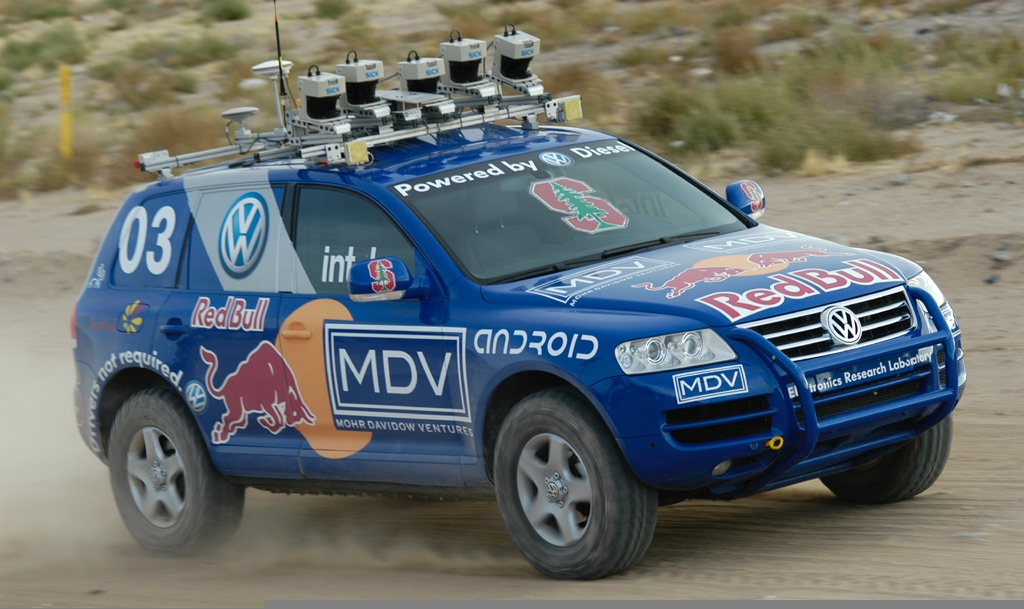
\includegraphics[width=0.8\linewidth]{1_darpa_winner_2005.png}
	\caption{Stanley, 2005 DARPA Grand Challenge winner}
	Source: \textit{Stanford university}
	\label{fig:1_darpa_winner_2005}
\end{figure}

Nevertheless, the first truly autonomous cars appeared in the 1980s with Carnegie Mellon University’s Navlab and ALV projects funded by the USA company DARPA (Defense Advanced Research Projects Agency) in 1984 and EUREKA Prometheus project (1987) developed by Mercedes-Benz and Bundeswehr University Munich’s. By 1985, the ALV project had shown self-driving speeds on two-lane roads of 31 km/h with obstacle avoidance added in 1986 and off-road driving in day and night conditions by 1987. Furthermore, from the 1960s through the second DARPA Grand Challenge in 2005 (212 km off-road course near the California-Nevada state line, surpassed by all but one of the 23 finalists), automated vehicle research in the United States was primarily funded by DARPA, the US Army and US Navy, yielding rapid advances in terms of speed, car control, sensor systems and driving competence in more complex conditions. This caused a boost in the development of autonomous prototypes by companies and research organizations, most of them from the United States. Figure \ref{fig:1_darpa_winner_2005} shows Stanley, the 2005 DARPA Gran Challenge winner, from Stanford university. \\

Even though self-driving cars have not yet displaced conventional cars, there can be found several examples of how it has become a hot topic for powerful companies such as Delphi Automotive Systems, Audi, BMW, Tesla, Mercedes-Benz or Waymo. \\

In 2005 Delphi broke the Navlab’s record achievement (driving 4,584 km while remaining 98 \% of the time autonomously) by piloting an Audi, improved with Delphi technology, over 5,472 km through 15 states while remaining in self-driving mode 99 \% of the time. Moreover, in 2005 the USA states of Michigan, Virginia, California, Florida, Nevada and the capital, Washington D.C., allowed the testing of automated cars on public roads. \\

In 2017, Audi stated that its A8 car prototype would be automated at speeds up to 60 km/h by using its perception system named “Audi AI”.  Also, in 2017 Waymo (self-driving technology development company subsidiary of Alphabet Inc) started a limited trial of a self-driving taxi service in Phoenix, Arizona. \\

Figure \ref{fig:1_disengagement_2020} shows the total number of autonomous test miles and miles per disengagement in California (Dec 2019 - Nov 2020) by some of the most important \ac{AD} technology development companies around the world. The concept disengagement is quite useful to assess the quality of an \ac{ADS}, defined as the deactivation of the autonomous mode when a failure of the autonomous technology is detected or when a safe operation requires that the autonomous vehicle test driver disengages the autonomous mode, resulting in control being seized by the human driver.

\begin{figure}[ht]
	\centering
	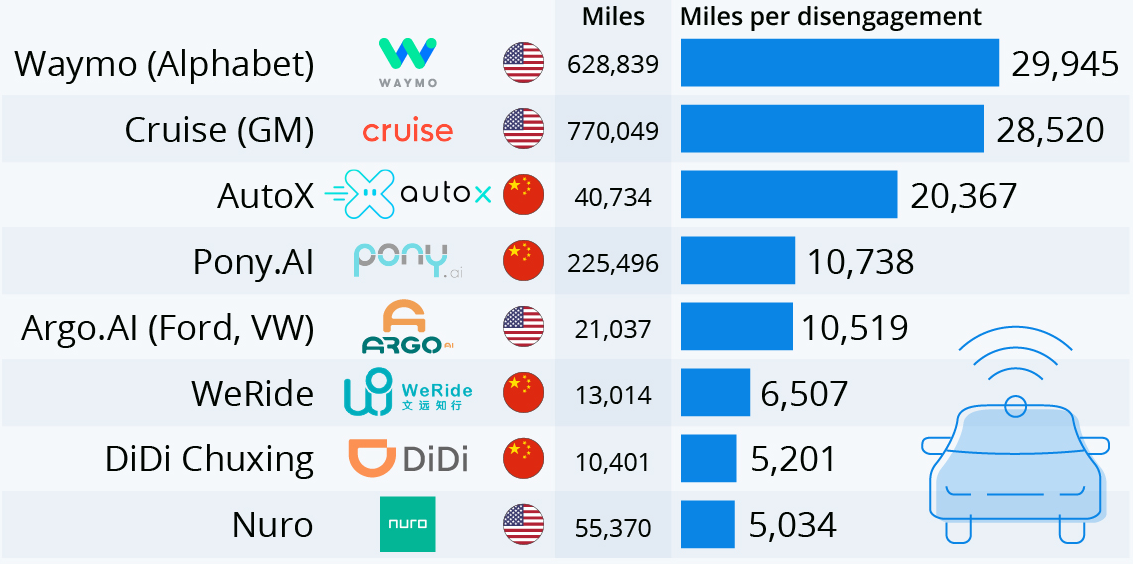
\includegraphics[width=0.6\linewidth]{1_disengagement_2020.png}
	\caption{Number of autonomous test miles and miles per disengagement (Dec 2019 - Nov 2020)}
	Source: \textit{DMV California, via The Last Driver License Holder}
	\label{fig:1_disengagement_2020}
\end{figure}

At the moment of writing this thesis (2023), many vehicles on the road are considered to be semi-autonomous due to safety features like braking systems, assisted parking, lane boundaries detection or predict the long-term behaviour of the users around the vehicle to execute the most optimal action in a safely way. Regarding this, the Society of Automotive Engineers (SAE) published the concept of autonomy levels in 2014, as part of its "Taxonomy and Definitions for Terms Related to On-Road Motor Vehicle Automated Driving Systems" report. Figure \ref{fig:1_nhtsa_sae_automation_levels} illustrates the six levels of autonomy (the higher the level, the more autonomous the car is), where it can be appreciated that Level Zero means "No Automation", being the acceleration, braking and steering controlled by a human driver at all times, and Level Five represents Full Automation, where there is a full-time automation of all driving tasks on any road, under any conditions, whether there is a human on board or not.

\begin{figure}[h]
	\centering
	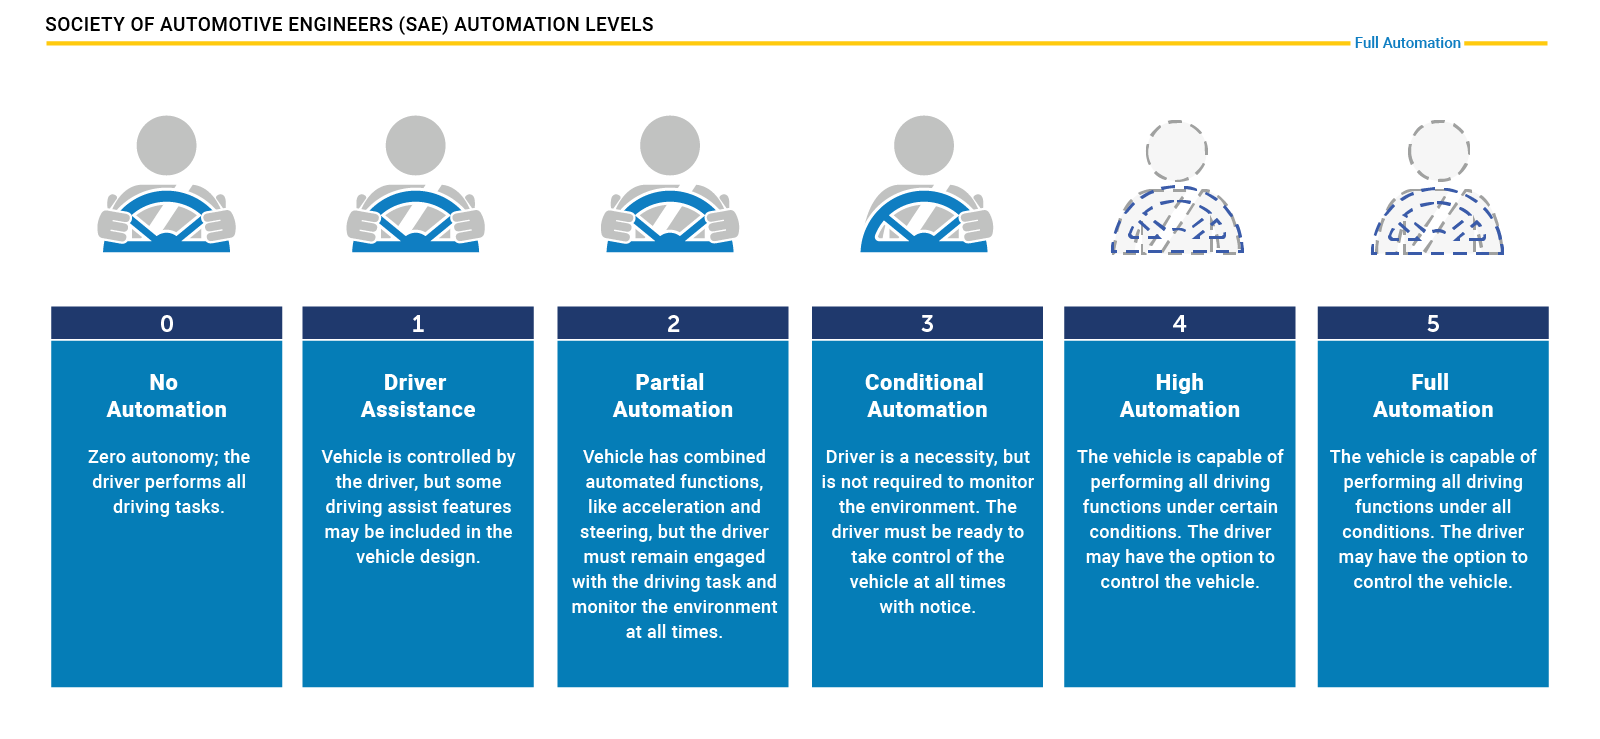
\includegraphics[width=0.8\linewidth]{1_nhtsa_sae_automation_levels.png}
	\caption{Society of Automotive Engineers (SAE) automation levels}
    Source: \textit{NHTSA (National Highway Traffic Safety Administration)}
	\label{fig:1_nhtsa_sae_automation_levels}
\end{figure}

In that sense, today most vehicles only included basic Advanced Driver Assistance Systems (ADAS), but major advancements in AD capabilities are on the horizon. According to a 2021 McKinsey consumer survey, growing demand for \ac{AD} systems could create billions of dollars in revenue. Based on a consumer interest in \ac{AD} features and commercial solutions available on the market today, ADAS and AD could generate between \$300 and \$400 billions in the passenger car market by 2035. Figure \ref{fig:1_mckinsey_revenues_ad} illustrates an interesting study reporting the revenues of ADAS and AD from Level 1 (Driver Assistance) to Level 4 (High Automation). As expected, Level 5 is excluded from this study due to the huge difficulties the automotive companies would have to face to adapt their systems under totally different environmental conditions.

\begin{figure}[h]
	\centering
	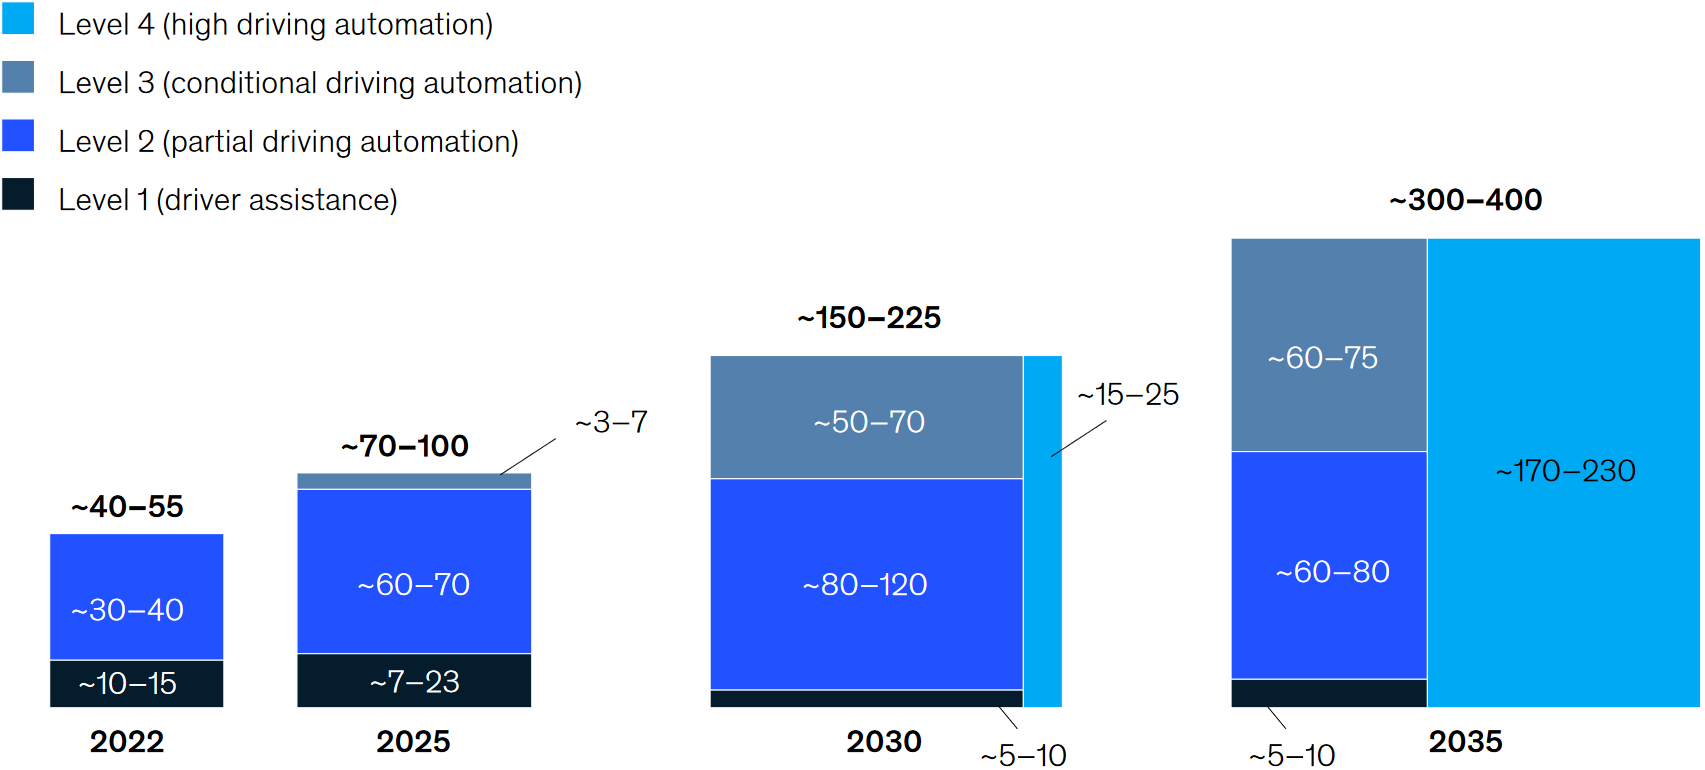
\includegraphics[width=0.8\linewidth]{1_mckinsey_revenues_ad.png}
	\caption{Advanced Driver Assistance systems (ADAS) and \\ Autonomous Driving (AD) revenues in \$ billion} Source: \textit{McKinsey Center for Future Mobility}
	\label{fig:1_mckinsey_revenues_ad}
\end{figure}

\section{Autonomous Driving architecture}
\label{sec:1_ad_architecture}

To sum up what commented above, increasing the level of autonomous navigation in mobile robots (from agriculture to public and private transport) are expected to create tangible business benefits to those users and companies employing them. However, designing an autonomous navigation system does not seem to be an easy task. In the \ac{SOTA} we can distinguish two main kind of software architectures: End-to-End and modular. Figure \ref{fig:1_ete_modular} illustrates the entire \ac{AD} architecture starting from sensing, all the way to longitudinal (throttle/brake) and lateral (steering angle) control of the vehicle, which are the commanded signals that feed the low-level electronic system that moves the vehicle, like a drive-by-wire system \cite{arango2020drive}. End-to-End are considered black-box models, where a single neural network performs the driving task (throttle/steering/brake) from raw sensor data, in such a way the error be may vanished since intermediate representations are jointly optimized, but these are not very interpretable. On the other hand, modular architectures (considered as glass models as counterpart to End-to-End approaches) separate the driving task into individually programmed or trained modules. This solution is more interpretable, since the know-how of a research group or company is easily transferred, they allow parallel development, being the standard solution in industrial research, but the error is propagated, where intermediate representations can led to suboptimal performance. For example, incorrect object detection can lead to low-quality tracking and motion prediction.

\begin{figure}[h]
	\centering
	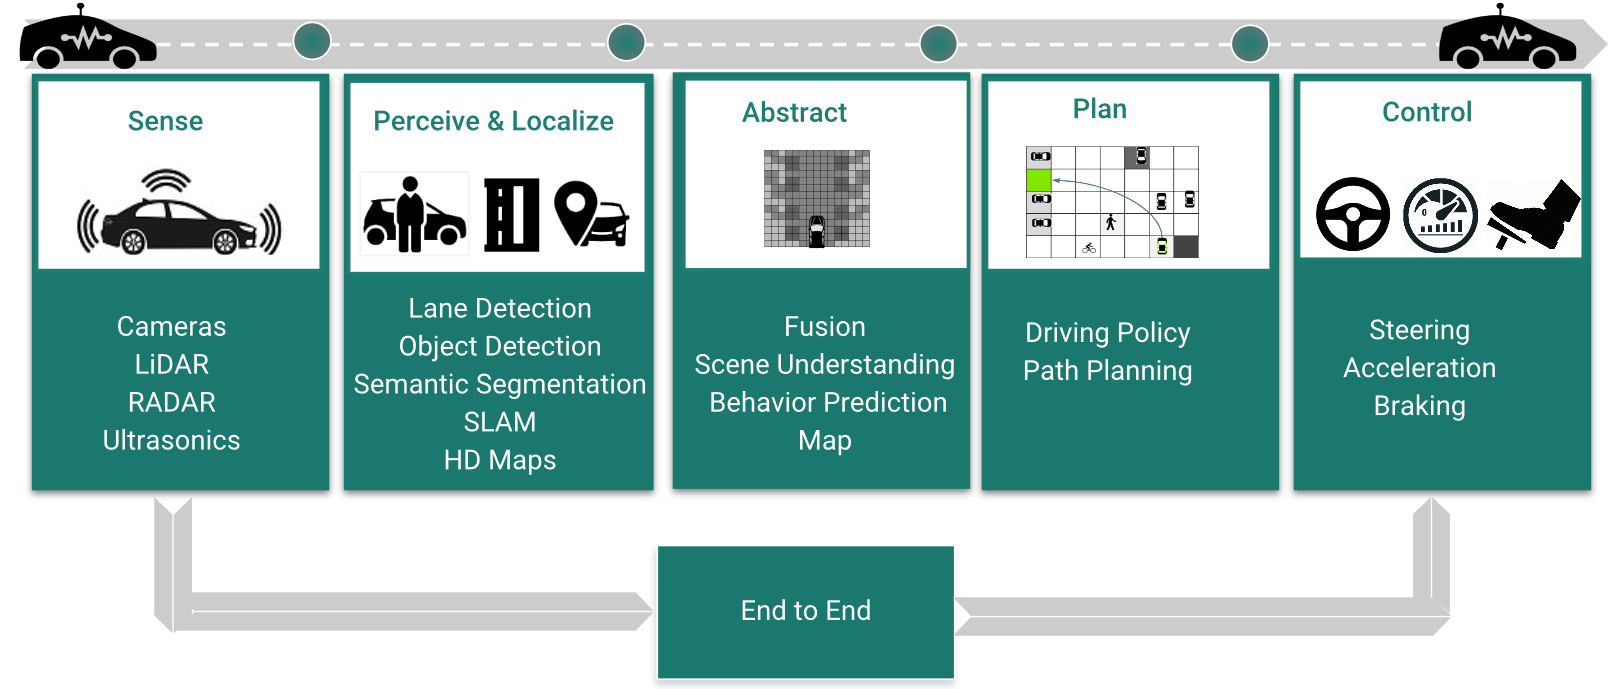
\includegraphics[width=0.8\linewidth]{1_ete_modular.png}
	\caption{Autonomous Driving Stack (ADS) modular vs end-to-end pipeline}
	Source: \textit{Vrunet: Multi-task learning model for intent prediction of vulnerable road users} \cite{ranga2020vrunet}
	\label{fig:1_ete_modular}
\end{figure}

Considering the RobeSafe (Robotics and eSafety) research group and the main projects (Techs4AgeCar, AIVATAR) where this thesis has been developed, we integrate our algorithms in a software modular approach. An example of a software modular approach is shown in Figure \ref{fig:1_pylot_architecture}. Despite the fact in literature some authors disagree on the specific software architecture of an \ac{ADS}, specially the motion prediction module, which is usually classified as a perception algorithm but sometimes is included as part of the planning or decision-making layers, we can hierarchically break down (from raw data to the driving task) a standard \ac{AD} architecture into the following software layers:

\begin{itemize}
	\item Localization layer: Positions and locates the vehicle on a map with real-time and centimetric accuracy approach. The main source of information is a robust differential-GNSS, though IMUs, wheel odometry and even cameras are commonly employed. 
	\item Perception layer: Understand the environment around the ego-vehicle thanks to the information collected by the sensors. If defined as multi-stage, the perception layer first detects the most relevant obstacles, then track them over time to finalize long-term predict with plausible predictions. In order to perform object detection, LiDAR, camera and RADAR are the main sensors that provide the corresponding raw data. Additionally, HD map information is frequently used in the motion prediction tasks by most \ac{SOTA} algorithms.
	\item Mapping layer: Responsible for creating a topologic, semantic and geographical modeling of the environment through which the vehicle drives, being the HD Map graph the most common source of information.
	\item Planning layer: This layer is comprised of three components: route, behaviour and trajectory planner. The route planner computes the most optimal (in terms of distance, time and so forth and so on) global route from some predefined start and goal. It uses the localization and mapping output. On the other hand, the behaviour planner, also referred as decision-making layer by some authors, it performs high-level decision-making of driving behaviours such as lane changes or progress through intersections, mostly focused on the previously computed global route and current localization. It can be seen as an atomization of the global route in different behaviors to reach the goal. Finally, the trajectory planner, also known as local planner, generates a time schedule for how to follow a path given constraints such as position, velocity and acceleration in order to meet the previously decided behaviour and taking into account the prediction from the perception layer, avoiding obstacles in optimal direction and speed conditions.
	\item Control layer: Once the local plan is calculated, the control layer is responsible for generating the commands that are sent to the actuators. It receives as input some waypoints from the calculations made in the trajectory planner. Once these waypoints are received, most authors perform spline interpolations and a velocity profile that ensures a smooth and continous trajectory. 
\end{itemize}

\begin{figure}[h]
	\centering
	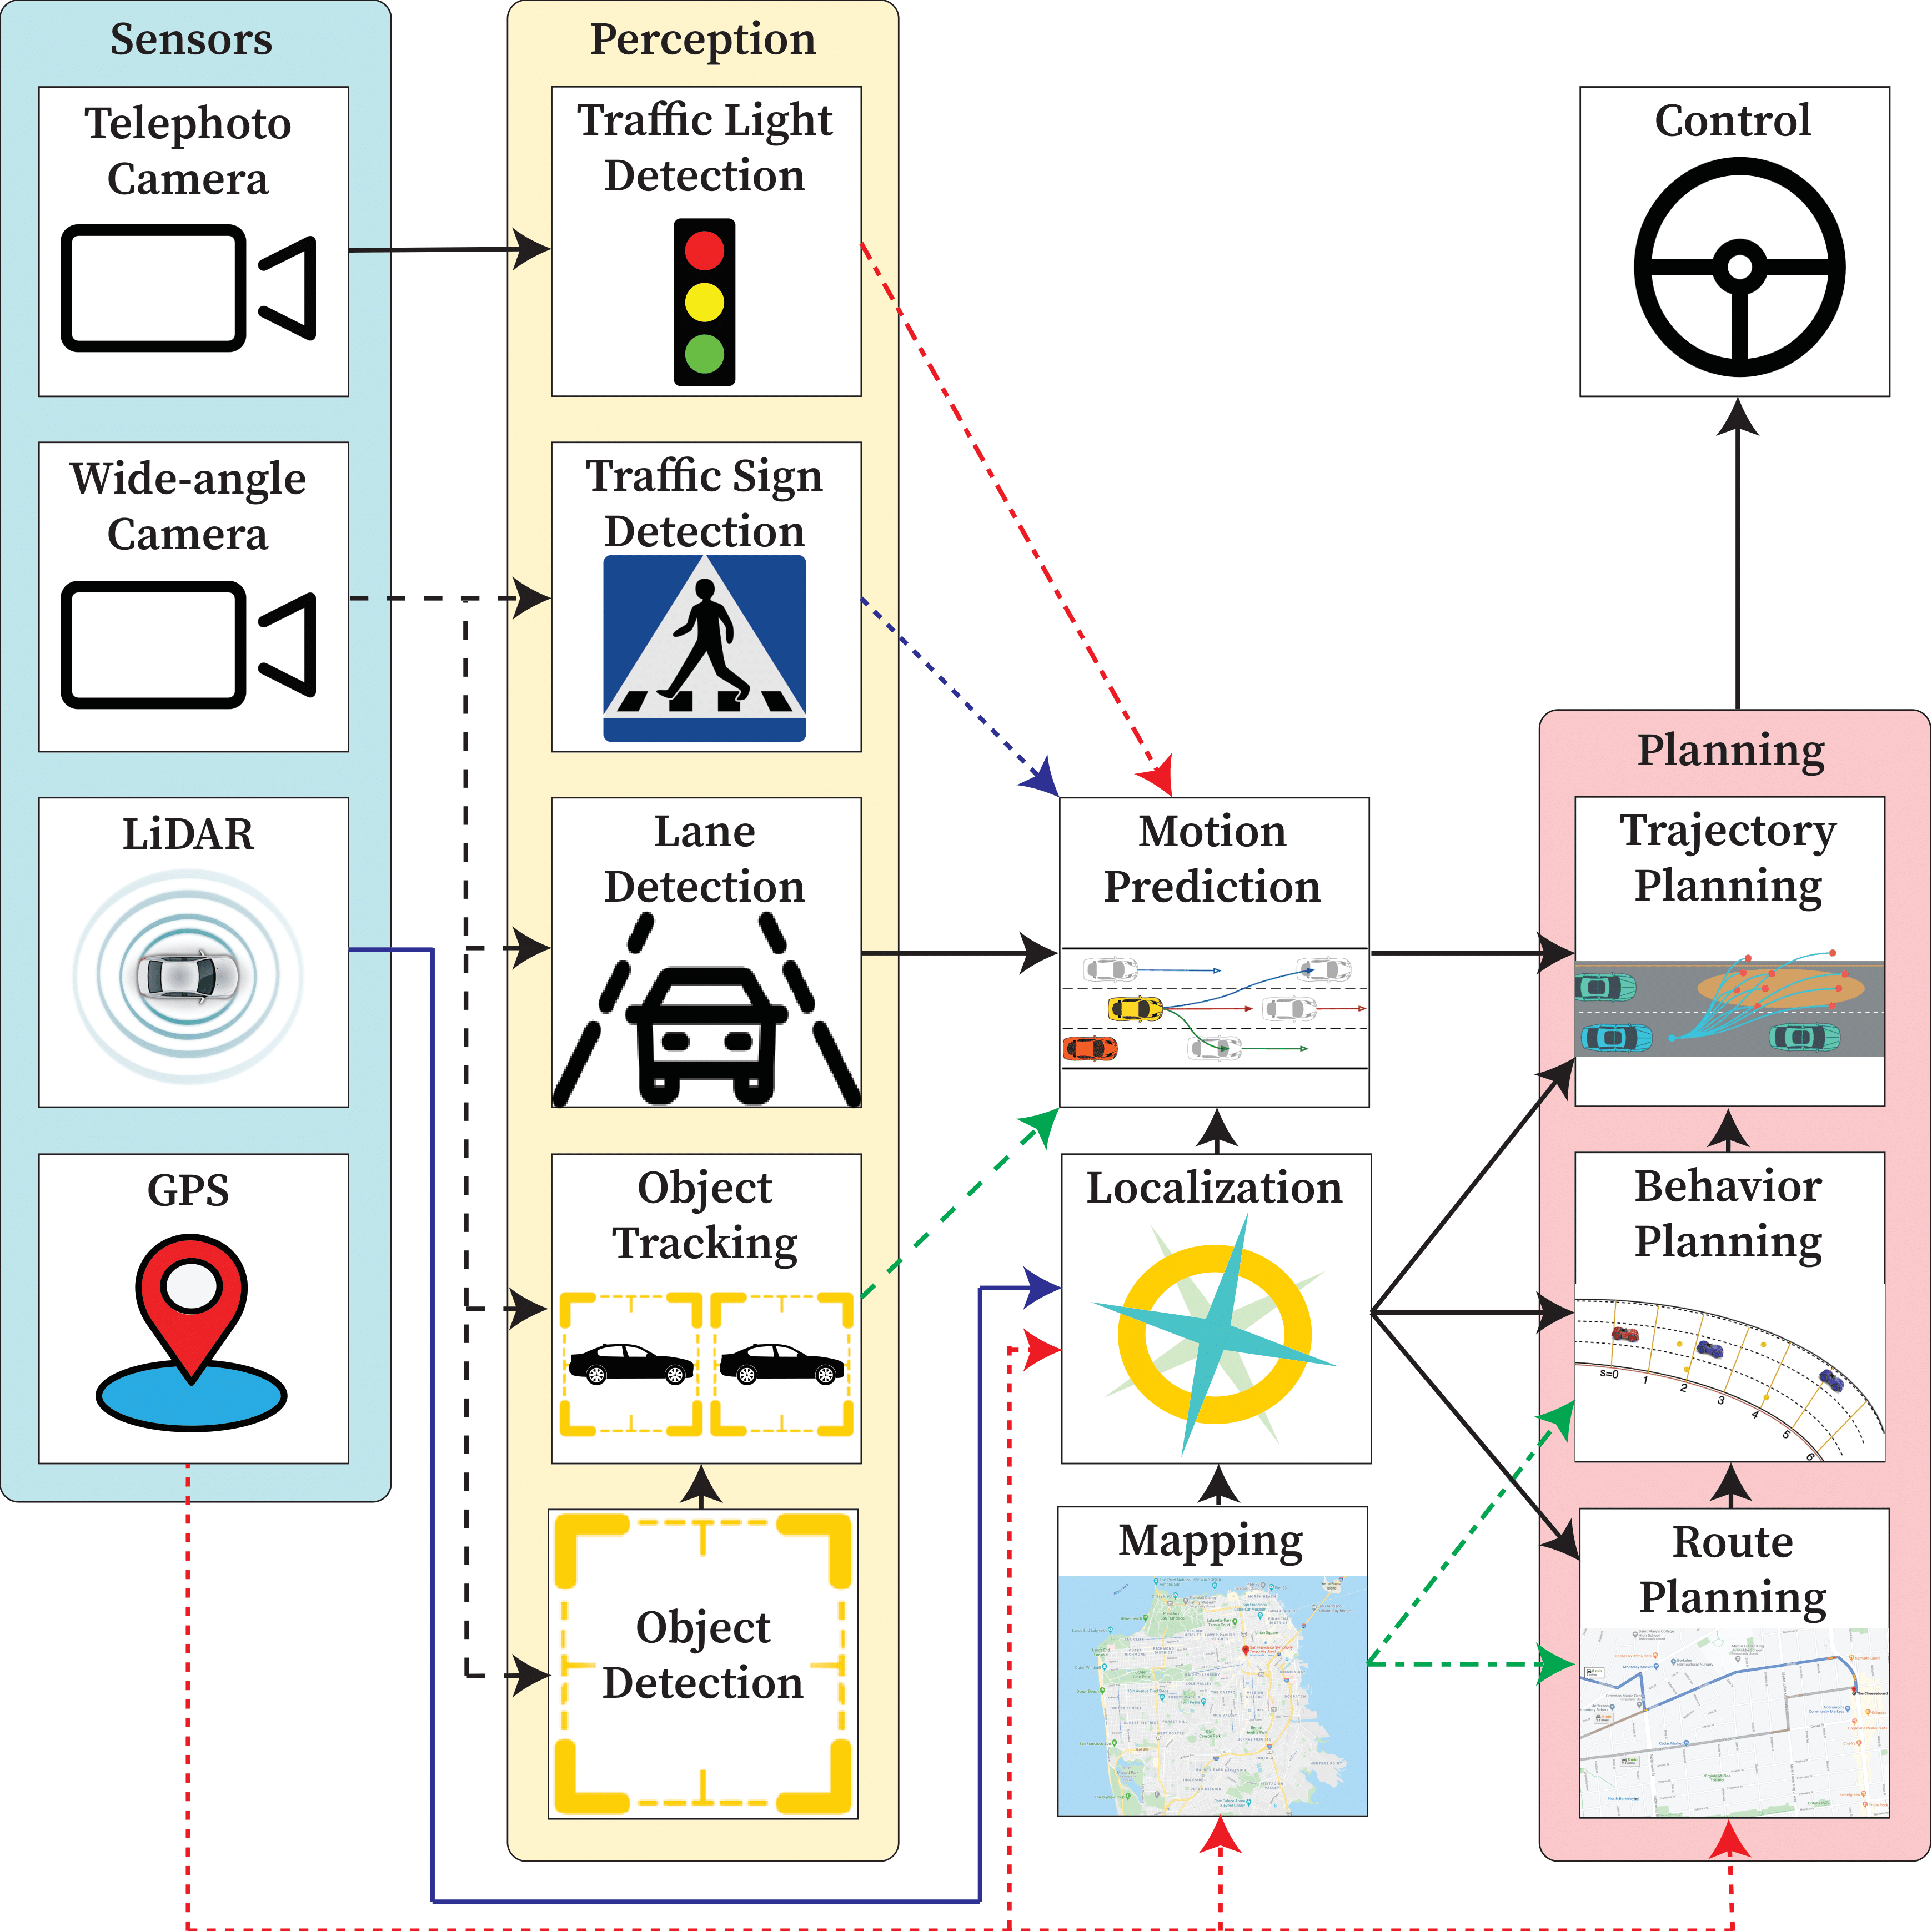
\includegraphics[width=0.8\linewidth]{1_pylot_architecture.png}
	\caption{Autonomous Driving Stack (ADS) modular pipeline}
	Source: \textit{Pylot: A modular platform for exploring latency-accuracy tradeoffs in autonomous vehicles} \cite{gog2021pylot}
	\label{fig:1_pylot_architecture}
\end{figure}

\section{Problem statement}
\label{sec:1_problem_statement}

As commented in previous sections, in order to operate efficiently and safely in highly dynamic, complex and interactive driving scenarios, \acs{ADS} need to smartly reason like human beings via predicting future motions of surrounding traffic participants during navigation. Nevertheless, achieving accurate and robust \ac{MP} in one of the most difficult and interesting challenges to achieve full-autonomy, since it is equivalent to a bridge between the former stages of the perception layer, where the scene is understood detecting and tracking static and dynamic objects of the environment, and the planning and control layer, where the future trajectory of the ego-vehicle is computed and the driving commands are sent to the physical layer (e.g. Drive-by-Wire \cite{arango2020drive}). Here are some of the most important challenges: 

\begin{enumerate}
	\item Heterogeneity of traffic participants. Traffic partipants (specially those which are dynamic) can be roughly classified as cyclists, pedestrians or other vehicles. The prediction model should be capable of differentiating the motion patterns of heterogeneous traffic participants, in such a way fine-grained classification (detection module) is quite beneficial to include additional metadata along with the past observations.
	\item Complexity of road structure. Road structures are highly diverse and complex, specially in highways and urban areas, which noticeably affect the motion behaviours of traffic participants.
	\item Variable number of interactive agents. The prediction model must deal with a number of associated traffic participants within a certain area that can vary from time to time, such as intersections or roundabouts. Then, while driving, a comprehensive representation of the scene must be able to accommodate an arbitrary number of involved traffic participants.
	\item Multimodality of driving behaviours. In real-world, despite we know the behaviour our vehicle will carry out, the motion patterns of other traffic participants can be considered inherently multimodal since there is usually more than one reasonable option for a driver to choose, specially in intersections, when the number of lanes increases or even in the same lane with different velocity profiles (constant velocity, sudden break, sudden acceleration). In that sense, a robust and reliable \ac{MP} model is expected to be human-like and capture different plausible motion modalities where an agent can travel in the prediction horizon.
	\item Complex interpendencies among traffic participants and road infrastructure. Agent-Agent, Agent-Road and Road-Road interpendencies are of great importance for \ac{MP} and interaction modeling, even more taking into account the complexity of road structures and heterogeneity of traffic participants aforementioned. As expected, an agent future trajectory will be affected not only by its own past trajectory and driving objectives (given by the behaviour planner) but also by other surrounding agents past trajectories, traffic rules and physical constraints.
\end{enumerate}

\section{Objectives and Structure of this Thesis}
\label{sec:1_objectives_and_structure}

The main scope of this thesis is to study the \ac{SOTA} and development of novel and efficient interaction-aware Deep Learning based \ac{MP} models, focusing on long-term (from 3 to 6 s) prediction horizon and \ac{AD}, where traffic participants can range from trucks to pedestrians, instead of models focused on pedestrian trajectory prediction. The main inputs that will be used throughout this work are the physical (map) information and historical states (that may include agent position, velocity, orientation, object type and category) of traffic participants in \ac{BEV}, assuming these objects have been previously tracked by our ego-vehicle (also referred as the autonomous car). Though the evaluation of these methods will be done using a single target agent, as proposed by some of the most important prediction datasets, like Argoverse 1 \cite{chang2019argoverse} and Argoverse 2 \cite{wilson2023argoverse}, some of the proposed methods will be trained considering multi-agent. In this thesis, the solutions to the aforementioned challenges will be discussed and investigated progressively. In order to achieve the main scope, the following objectives will be met:

\begin{enumerate}
	\item Research of \ac{SOTA} \ac{MP}, focused on \ac{DL} and the \ac{AD} paradigm.
	\item Propose of several \ac{MP} architectures, studying the progressive incorporation of \ac{DL} mechanisms and different sources of information and metadata, achieving \ac{SOTA} accuracy while reducing in millions of parameters previous models as well as inference time.
	\item Validate the proposed models in downstream applications, such as decision-making or behaviour planning, taking into account former stages of the perception layer (detection and tracking) instead of static files (benchmarks) in hyper-realistic simulation, as a preliminary stage before implementing it in a real-world vehicle.
\end{enumerate}

The organization of this document has been done as follows:

\begin{itemize}
	\item Chapter 2 reviews the most important features and methods of physics-based and learning-based \ac{MP} methods. The physics-based methods are reviewed according to a taxonomy similar to existing reviews. The learning-based methods are reviewed based on two classification criteria: scene representation and trajectory decoding.
	\item Chapter 3 presents a technical background, mostly focused on \ac{DL} mechanisms to deal with temporal sequences and interactions, to deeply understand the proposed methods.
	\item Chapter 4 illustrates the different prediction models developed in the thesis using different validation environments, from unimodal physic-based prediction to the final model of the thesis which takes into account agents interactions, map information and past observations using a novel scene representation with heuristic proposals, graph-based encoding, \ac{DL}-based goal proposals and motion refinement.
	\item Chapter 5 addresses the integration of the final model of the thesis with upstream and downstream modules to contribute the entire pipeline and closed-loop for \ac{AD}.
	\item Chapter 6 summarizes the thesis and provides some promising directions for future work in the areas of \ac{MP} and validation.
\end{itemize}

%%%%%%%%%%%%%%%%%%%%%%%%%%%%%%%%%%%%%%%%%%%%%%%%%%%%%%%%%%%%%%%%%%%%%%%%%%% 
% 
% Generic template for TFC/TFM/TFG/Tesis
% 
% By:
% + Javier Macías-Guarasa. 
% Departamento de Electrónica
% Universidad de Alcalá
% + Roberto Barra-Chicote. 
% Departamento de Ingeniería Electrónica
% Universidad Politécnica de Madrid   
% 
% Based on original sources by Roberto Barra, Manuel Ocaña, Jesús Nuevo,
% Pedro Revenga, Fernando Herránz and Noelia Hernández. Thanks a lot to
% all of them, and to the many anonymous contributors found (thanks to
% google) that provided help in setting all this up.
% 
% See also the additionalContributors.txt file to check the name of
% additional contributors to this work.
% 
% If you think you can add pieces of relevant/useful examples,
% improvements, please contact us at (macias@depeca.uah.es)
% 
% You can freely use this template and please contribute with
% comments or suggestions!!!
% 
%%%%%%%%%%%%%%%%%%%%%%%%%%%%%%%%%%%%%%%%%%%%%%%%%%%%%%%%%%%%%%%%%%%%%%%%%%% 

\chapter{Related Works}
\label{cha:related_works}

begin{FraseCelebre}
\begin{Frase}
	Llegaré a ser el mejor, El mejor que habrá jamás \\
	Mi causa es ser su entrenador, Tras poderlos capturar.  
	
	Viajaré a cualquier lugar, Llegaré a cualquier rincón \\  
	Y al fin podré desentrañar, El poder de su interior.  
	
	¡Pokémon! Hazte con todos (solos tú y yo), \\
	Es mi destino, mi misión \\
	¡Pokémon! Tú eres mi amigo fiel, \\
	Nos debemos defender.
\end{Frase}
\begin{Fuente}
	Opening 1 de Pokémon: "Gotta catch 'em all!" \\
	Autor original: Jason Paige
\end{Fuente}
\end{FraseCelebre}

One of the crucial tasks that \acp{ADS} must face during navigation, specially in arbitrarily complex urban scenarios, is to predict the behaviour of dynamic obstacles \cite{chang2019argoverse, salzmann2020trajectron++}. In a similar way to humans that pay more attention to nearby obstacles and upcoming turns than considering the obstacles far away, the perception layer of an \ac{ADS} must focus more on the salient regions of the scene, particularly on the more relevant dynamic agents to predict their future behaviour before conducting a maneuver, such as lane changing or accelerating. In that sense, before proceeding with the study of the different methods of the \ac{SOTA} of \ac{MP} in the field of \ac{AD}, one important thing to note is that this thesis is focused on non-conditional motion prediction, also referred as Passive Motion Prediction (PMP), where the prediction of surrounding agents is not influenced by the future decisions of the ego-vehicle or even other agents, referred as Conditional Motion Prediction (CMP) in the literature. Most existing works \cite{gilles2021home, gilles2022gohome, varadarajan2022multipath++, wang2022ganet, schmidt2022crat, liang2020learning} focus on a passive prediction scheme, where the future states of a particular agent are predicted given its past information, other surrounding agents information and interactions as well as the physical context. Then, downstream planning modules, specially the behaviour planning module (also referred as decision-making layer, as stated in Section \ref{sec:1_ad_architecture}), the ego-vehicle (our vehicle) future actions are computed according to the predicted trajectories in a passive manner, that is, without modifying the output of the prediction model, and the global route previously calculated. \\

\begin{figure}[h]
	\centering
	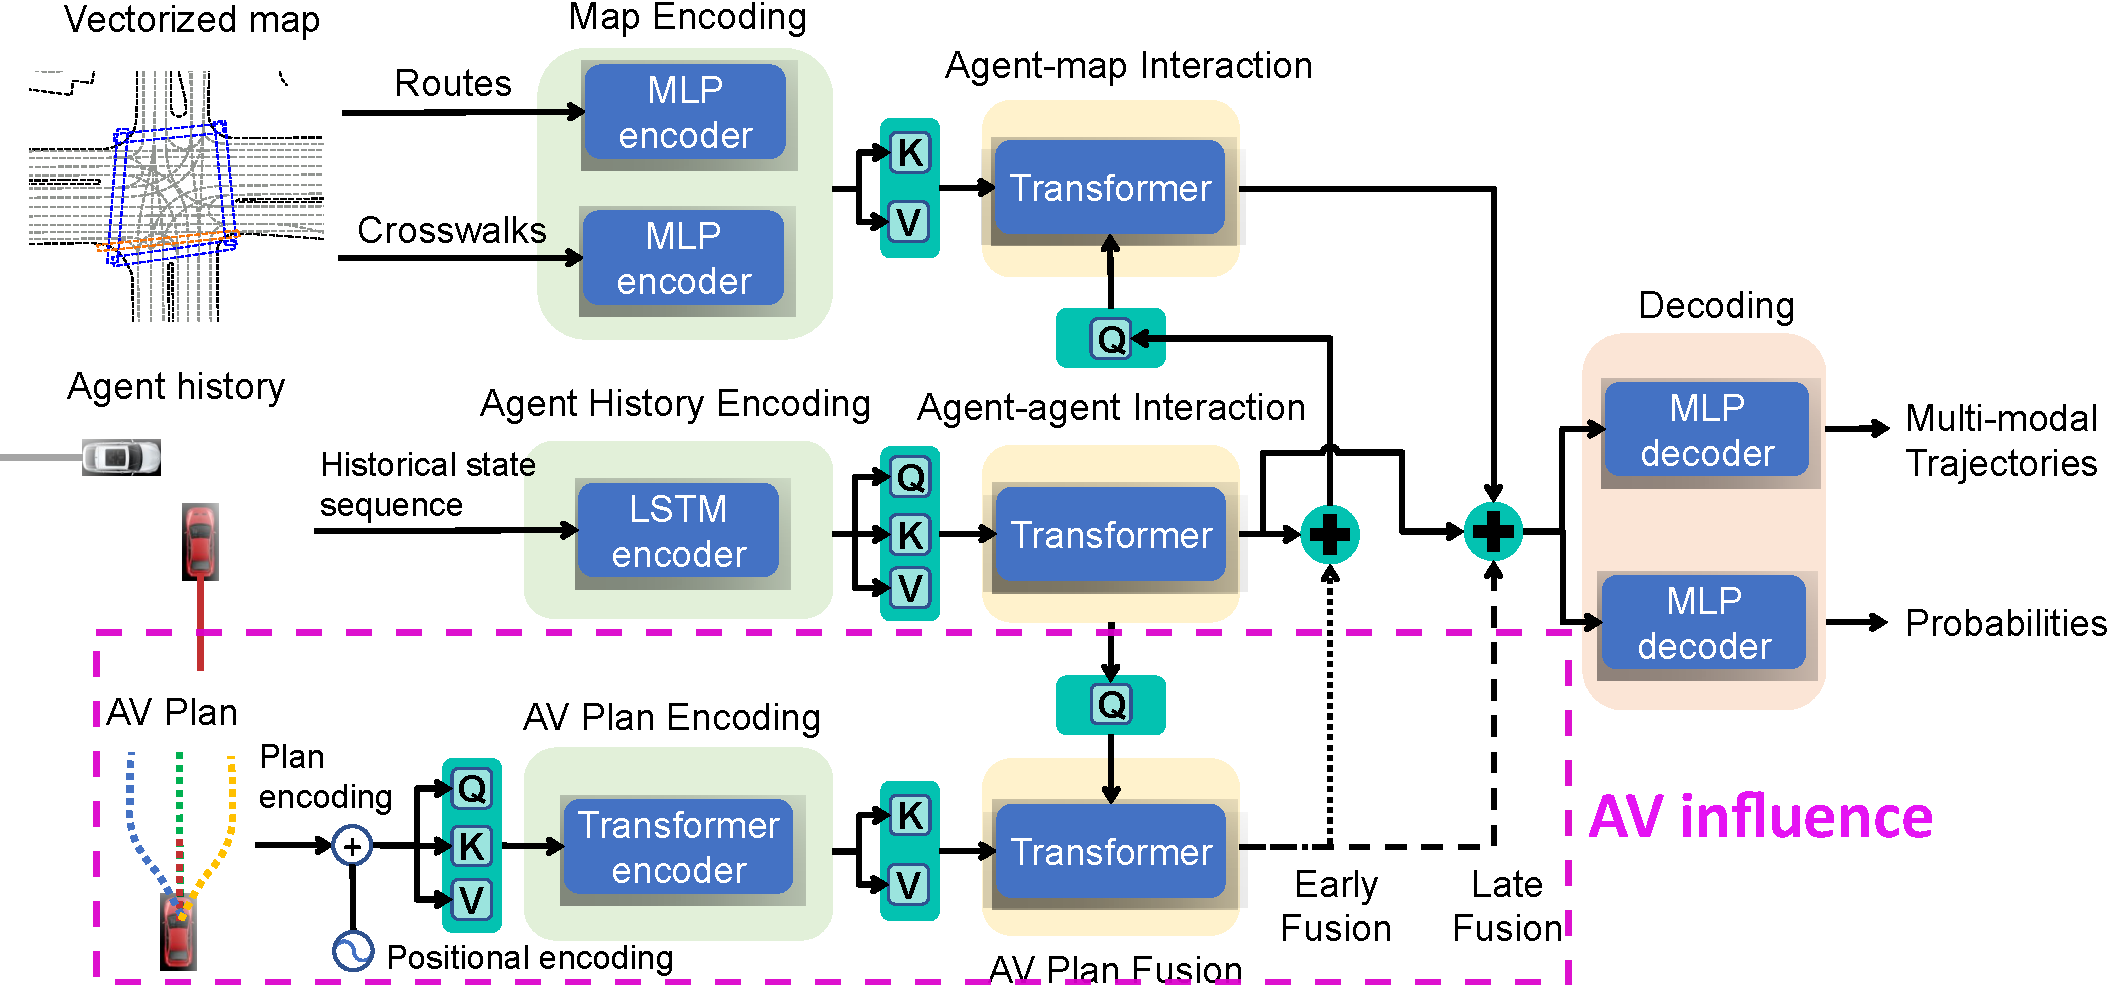
\includegraphics[width=0.8\linewidth]{2_cmp_vs_pmp.pdf}
	\caption{Example of a Conditional Motion Prediction (CMP) network. We \textcolor{magenta}highlight the influence of the \ac{AD} in the prediction of surrounding agents}
	Source: \textit{Conditional Predictive Behavior Planning with Inverse Reinforcement Learning for Human-like Autonomous Driving} \cite{huang2023conditional}
	\label{fig:2_cmp_vs_pmp}
\end{figure}

Nevertheless, to ensure safety under various predicted trajectories of the surrounding agents, our \ac{ADS} must overly conservative with inefficient maneuvers, specifically in arbitrarily complex traffic scenarios, because passive \ac{MP} models ignore the fact that the future states of an agent can influence the future actions of other agents, what is the most realistic situation. To this end, researchers recently started to explore a more coherent interactive prediction and planning framework which relies on predicting the surrounding agents future trajectories conditioned on the ego-vehicle future actions \cite{tang2019multiple} \cite{rhinehart2019precog} \cite{khandelwal2020if}, as a preliminary state to implement a fully-interaction graph where the future states of all agents (either autonomous prototypes or human-driven) influence in the decision of all agents. Under such frameworks, the \acs{ADS} can reason over potential actions while considering its influence on surrounding agents, as observed in Figure \ref{fig:2_cmp_vs_pmp}, inducing less conservative and more efficient maneuvers in highly interactive scenarios. \cite{huang2023conditional} propose a learning-based behaviour planning framework that learns to predict conditional multi-agent future trajectories, evaluating decisions from real-world human data. Moreover, they propose a two-stage learning process where the prediction model is trained first conditioned on the \ac{ADS} future actions, and then used as an environment model in the learning of the cost function with maximum entropy Inverse Reinforcement Learning (IRL). \cite{tang2022interventional} argue that CMP-based models essentially learns the posterior distribution of future trajectories conditioned on the future states of the ego-vehicle, where this future trajectory is treated as an observation, whilst safe and realistic prediction models should build the \ac{MP} to approximate the future trajectory distribution under the intervention of enforcing the \ac{ADS} future states, referring this new task as Interventional Behaviour Prediction (IBP). As aforementioned, the algorithms developed throughout this thesis do not focus on the joint study of the prediction and behaviour planning modules, but on studying efficient and powerful PMP algorithms without considering the future states of the autonomous agents as an additional condition. \\

Once the difference between CMP and PMP is stated












Most traditional predictions methods \cite{huang2022survey}, which usually only consider physics-related factors (like the velocity and acceleration of the target vehicle that is going to be predicted) and road-related factors (prediction as close as possible to the road centerline), are only suitable for \textbf{short-time} prediction tasks \cite{huang2022survey} and simple traffic scenarios, such as constant velocity (CV) in a highway or a curve (Constant Turn Rate Velocity, CTRV) where a single path is allowed, i.e. multiple choices computation are not required. Recently, MP methods based on DL have become increasingly popular since they are able not only to take into account these above-mentioned factors but also consider interaction-related factors (like agent-agent \cite{gupta2018social}, agent-map \cite{casas2018intentnet} and map-map \cite{liang2020learning}) in such a way the algorithm can adapt to more complex traffic scenarios (intersections, sudden breaks and accelerations, etc.). It must be consider that multimodal, specially in the field of vehicle motion prediction, does not refer necessarily to different directions (e.g. turn to the left, turn to the right, continue forward in an intersection), but it may refer to different predictions in the same direction that model a sudden positive or negative acceleration, so as to imitate a realistic human behaviour in complex situations. As expected, neither classical nor Machine Learning (ML) methods can model these situations \cite{huang2022survey}.

\begin{table*}[t]
	\begin{center}
		\caption{Main state-of-the-art methods for Motion Prediction. Main categories are Encoder (splitted into motion history, social info (agent interactions) and map info (physical information)), Decoder, Output representation and Distribution over future trajectories.}
		%\begin{tabular}{| c | cccccc |}
		%\begin{tabular}{| c | cccccc |}
		\begin{tabular}{r |ccc|c|c|c}
			
			\toprule
			\textbf{Method}	&	& \textbf{Encoder}	&	& \textbf{Decoder}	& \textbf{Output}  & \textbf{Trajectory Distribution}	\\
			& Motion history	& Social info	& Map info	&	&	&	\\
			\midrule
			\midrule
			SocialLSTM~\cite{alahi2016social}	& LSTM	& spatial pooling	& --	& LSTM	& states	& samples	\\
			SocialGan~\cite{gupta2018social}	& LSTM	& maxpool	& --	& LSTM	& states	& samples	\\
			Jean~\cite{mercat2020multiattentmotion}	& LSTM	& attention	& --	& LSTM	& states	& GMM	\\
			TNT~\cite{zhao2020tnt}	& polyline	& maxpool, attention	& polyline	& MLP	& states	& weighted set	\\
			LaneGCN~\cite{liang2020learninggraph}	& 1D-conv	& GNN	& GNN	& MLP	& states	& weighted set	\\
			WIMP~\cite{khandelwal2020if}	& LSTM	& GNN+attention	& polyline	& LSTM	& states	& GMM	\\
			VectorNet~\cite{gao2020vectornet}	& polyline	& maxpool, attention	& polyline	& MLP	& states	& unimodal	\\
			SceneTransformer~\cite{ngiam2021scene}	& attention	& attention	& polyline	& attention	& states	& weighted set	\\
			HOME~\cite{gilles2021home}	& raster	& attention	& raster	& conv	& states	& heatmap	\\
			GOHOME~\cite{gilles2021gohome}	& 1D-conv+GRU	& GNN	& GNN	& MLP	& states	& heatmap	\\
			MP3~\cite{casas2021mp3}	& raster	& conv	& raster	& conv	& cost function	& weighted samples	\\
			%CoverNet~\cite{phan2019covernet}	& raster	& conv	& raster	& lookup	& states	& GMM w/ dynamic anchors	\\
			%DESIRE~\cite{lee2017desire}	& GRU	& spatial pooling	& raster	& GRU	& states	& samples	\\
			ExploringGAN~\cite{gomez2022exploring}	& LSTM	& attention	& polyline	& LSTM	& states	& unimodal	\\
			% MFP~\cite{tang2019multiple}	& GRU	& RNNs+attention	& raster	& GRU	& states	& samples	\\
			%MANTRA~\cite{marchetti2020mantra}	& GRU	& --	& raster	& GRU	& states	& samples	\\
			%PRANK~\cite{biktairov2020prank}	& raster	& conv	& raster	& lookup	& states	& weighted set	\\
			%IntentNet~\cite{casas2018intentnet}	& raster	& conv	& raster	& conv	& states	& unimodal	\\
			Multimodal~\cite{cui2019multimodal}	& raster	& conv	& raster	& conv	& states	& weighted set	\\
			MultiPath~\cite{chai2019multipath}	& raster	& conv	& raster	& MLP	& states	& GMM w/ static anchors	\\
			MultiPath++~\cite{varadarajan2021multipath++}	& LSTM	& RNNs+maxpool	& polyline	& MLP	& control poly	& GMM	\\
			%PLOP~\cite{buhet2021plop}	& LSTM	& conv	& raster	& MLP	& state poly	& GMM	\\
			Trajectron++\cite{salzmann2020trajectron++}	& LSTM	& RNNs+attention	& raster	& GRU	& controls	& GMM	\\
			CRAT-PRED\cite{schmidt2022crat}	& LSTM	& GNN+attention	& --	& MLP	& states	& weighted set	\\
			%R2P2~\cite{rhinehart2018r2p2}	& GRU	& --	& polyline	& GRU	& motion	& samples	\\
			%DKM~\cite{cui2020deep}	& raster	& conv	& raster	& conv	& controls	& weighted set	\\
			\midrule					
			\textbf{Ours - Social baseline}	& LSTM	& GNN+attention	& --	& LSTM	& states	& weighted samples	\\
			\textbf{Ours - Map baseline}	& LSTM	& GNN+attention	& polyline 	& LSTM	& states	& weighted samples	\\
			\bottomrule
		\end{tabular}
		\label{table:related_work}
	\end{center}
\end{table*} 

In order to classify DL based MP methods, we distinguish several important features: Motion history, Social information (agent interactions), Map information (road encoding), how the model returns the output trajectory and its corresponding distribution. Table \ref{table:related_work} summarizes several SOTA methods, inspired in the survey proposed by \cite{varadarajan2021multipath++}.

\begin{itemize}
	
	\item \textbf{Motion history}: Most methods encode the sequence of past observed states using 1D-convolution \cite{liang2020learninggraph} \cite{mercat2020multiattentmotion}, able to model spatial information, or via a recurrent net \cite{gomez2022exploring} \cite{alahi2016social} (LSTM, GRU), which are more useful to handle temporal information. Other methods that use a raster version of the whole scenario represent the agent states rendered as a stack of binary mask images depicting agent oriented bounding boxes \cite{gilles2021home}. On the other hand, other approaches encode the past history of the agents in a similar way to the road components of the scene given a set of vectors or polylines \cite{zhao2020tnt, gao2020vectornet} that can model the high-order interactions among all components, or even employing attention to combine features across road elements and agent interactions \cite{ngiam2021scene}.
	
	\item \textbf{Social information}: In complex scenarios, motion history encoding of a particular target agent is not sufficient to represent the latent space of the traffic situation, but the algorithm must deal with a dynamic set of neighbouring agents around the target agent. Common techniques are aggregating neighbour motion history with a permutation-invariant set operator: soft attention \cite{ngiam2021scene, gomez2022exploring}, a combination of soft attention and RNN \cite{varadarajan2021multipath++} / GNN \cite{schmidt2022crat} or social pooling \cite{alahi2016social, gupta2018sgan}. Raster based approaches rely on 2D convolutions \cite{chai2019multipath} \cite{casas2021mp3} over the spatial grid to implicitly capture agent interactions in such a way long-term interactions are dependent on the neural network receptive fields.
	
	%quito la cita suelta \cite{murciego2018topological} para evitar self-citations en review y ahorrar 4 lineas. En el CR la puedes añadir.
	
	\item \textbf{Map information}: High-fidelity maps~\cite{can2022maps} have been widely adopted to provide offline information (also known as physical context) to complement the online information provided by the sensor suite of the vehicle and its corresponding algorithms. Recent learning-based approaches \cite{mahjourian2022occupancy, casas2018intentnet, ivanovic2021heterogeneous}, which present the benefit of having probabilistic interpretations of different behaviour hypotheses, require to build a representation to encode the trajectory and map information. Map information is probably the feature with the clearest dichotomy: raster vs vector treatment. The raster approach encodes the world around the particular target agent as a stack of images (generally from a top-down orthographic view, also known as Bird's Eye View). This world encoding may include from agent state history, agent interactions and usually the road configuration, integrated all this different-sources information as a multi-channel image \cite{gilles2021home}, in such a way the user can use an off-the-shelf Convolutional Neural Network (CNN) based pipeline in order to leverage this powerful information. Nevertheless, this representation has several downsides: constrained field of view, difficulty in modeling long-range interactions and even difficulty in representing continuous physical states due to the inherent world to image (pixel) discretization. On the other hand, the polyline approach may describe curves, such as lanes, boundaries, intersections and crosswalks, as piecewise linear segments, which usually represents a more compact and efficient representation than using CNNs due to the sparse nature of road networks. Some state-of-the-art algorithms not only describe the world around a particular agent as a set-of-polylines \cite{khandelwal2020if} \cite{zhao2020tnt} in an agent-centric coordinate system, but they also leverage the road network connectivity structure \cite{liang2020learninggraph} \cite{zeng2021lanercnn} treating road lanes as a set of nodes (waypoints) and edges (connections between waypoints) in a graph neural network so as to include the topological and semantic information of the map.
	
	% Additional bio: deo2018cstlstmpool, rhinehart2019precog
	
	\item \textbf{Decoder}: Pioneering works of DL based MP usually adopt the autoencoder architecture, where the decoder is often represented by a recurrent network (GRU, LSTM, etc., specially designed to handle temporal information) to generate future trajectories in an autoregressive way, or by CNNs \cite{gilles2021home} \cite{gilles2021gohome} / MLP \cite{liang2020learninggraph} \cite{schmidt2022crat} using the non-autoregressive strategy. The method may use an autoregressive strategy where the pipeline generates tokens (in this case, positions or relative displacements) in a sequential manner, in such a way the new output is dependent on the previously generated output, whilst MLP \cite{schmidt2022crat}, CNN \cite{gilles2021home} or transformer \cite{ngiam2021scene} based strategies usually follow a non-autoregressive strategy, where from a latent space the whole future trajectory is predicted.
	
	\item \textbf{Output}: The most popular model output representation is a sequence of states (absolute positions) or state differences (relative displacements for any dimension considered). The spacetime trajectory may be intrinsically represented as a continous polynomial representation or a sequence of sample points. Other works \cite{gilles2021home} \cite{gilles2021gohome} first predict a heatmap and then decode the corresponding output trajectories after sampling points from the heatmap, whilst \cite{casas2021mp3} \cite{zeng2019end} learn a cost function evaluator of trajectories that are enumerated heuristically instead of being generated by a learned model. 
	
	\item \textbf{Trajectory Distribution}: The choice of output trajectory distributions has several approaches on downstream applications. Regardless the agent to be predicted is described as a (non-)holonomic \cite{triggs1993motion} platform, an intrinsic property of the motion prediction problem is that the agent must follow one of a diverse set of possible future trajectories. A popular choice to represent a multimodal prediction are Gaussian Mixture Models (GMMs) due to their compact parameterized form, where mode collapse (associated frequently to GMMs) is addressed through the use of trajectory anchors \cite{chai2019multipath} or training  tricks \cite{cui2019multimodal}. Other approaches model a discrete distribution via a collection of trajectory samples extracted from a latent space and decoded by the model \cite{rhinehart2018r2p2} or over a set of trajectories (fixed or a priori learned) \cite{liang2020learninggraph}.
	
	% Additional bio: \cite{biktairov2020prank}
	
\end{itemize}

After classifying main SOTA methods, we conclude this section presenting the main characteristics of our baseline approaches. We make use of LSTM to encode the past motion history, GNN in combination with soft-attention the compute social interactions, a set-of-polylines to represent the most important map information and LSTM to decode the trajectories from the latent space. The output multimodal prediction is represented by a set of states with their corresponding confidences indicating the most plausible modes.
% Social LSTM \cite{alahi2016social} applies an LSTM autoencoder (adopting the NLL loss to model the error for each future step) whilst its generative continuation, Social GAN \cite{gupta2018social} uses an adversarial \cite{goodfellow2014gan} frame with social attention encoding the input trajectories with LSTM and then decoding different multiple modalities with the inherent noise associated to generative models, adopting per-step MSE loss. DESIRE \cite{lee2017desire} applies a conditional variational autoencoder in order to sample a diverse set of plausible modalities, making use of a GRU to generate the final predictions. 

% Moreover, SoPhie \cite{sadeghian2019sophie} represents one of the first DL based MP models that leverages two sources of information: the path states (position, velocity, heading, etc.) of all the agents in the scene and the physical context information, using Bird's Eye View (BEV) images as inputs and CNN as feature extractor. After fusing both physical and social attention, this model can successfully predict multiple acceptable trajectories that respect both social constraints (not collide with other agents) and physical constraints (most predictions are in the plausible area). Authors show that by modeling jointly the information about the physical environment and interactions between all agents, the model is able to learn better than when both sources of information are used independently

% In that sense, high-fidelity maps~\cite{can2022maps} have been widely adopted to provide offline information (also known as physical context) to complement the online information provided by the sensor suite of the vehicle and its corresponding algorithms. Recent learning-based approaches \cite{mahjourian2022occupancy, xiao2022multimodalend2end, casas2018intentnet, deo2018cstlstmpool, rhinehart2019precog, ivanovic2021heterogeneous}, which present the benefit of having probabilistic interpretations of different behaviour hypotheses, require to build a representation to encode the trajectory and map information. Hong et al.~\cite{hong2019rules} assumes that detections around the vehicle are provided and focuses on behaviour prediction by encoding entity interactions with ConvNets. \textbf{Intentnet}~\cite{casas2018intentnet} proposes to jointly detect traffic participants (mostly focused on vehicles) and predict their trajectories using raw LiDAR pointcloud and HD map information. %PRECOG~\cite{rhinehart2019precog} aims to capture the future stochasticity by flow-based generative models. 
%
% \textbf{MultiPath} by Chai et al.~\cite{chai2019multipath} uses ConvNets as encoder and adopts pre-defined trajectory anchors to regress multiple possible future trajectories.

% \textbf{HOME} by Gilles et al.~\cite{gilles2021home} presented a novel representation for multimodal trajectory prediction, where the model takes as input the context (map) and history of past trajectories, and generates an unconstrained 2D heatmap representation of the agent’s possible future trajectories, which represents the probability distribution of the agent’s future location. The method builds on simple architecture with classic convolution networks coupled with attention mechanism for agent interactions. Fig.~\ref{fig:prev_models} shows the SoPhie and HOME architectures. Both methods have two-streams, one for each input (trajectories and map), and use CNNs to process the map or physical context.

% In Section~\ref{sec:ours} we explain our solution to this trade-off problem.

\

\section{Introduction}
\label{sec:2_introduction}

\begin{figure}[h]
	\centering
	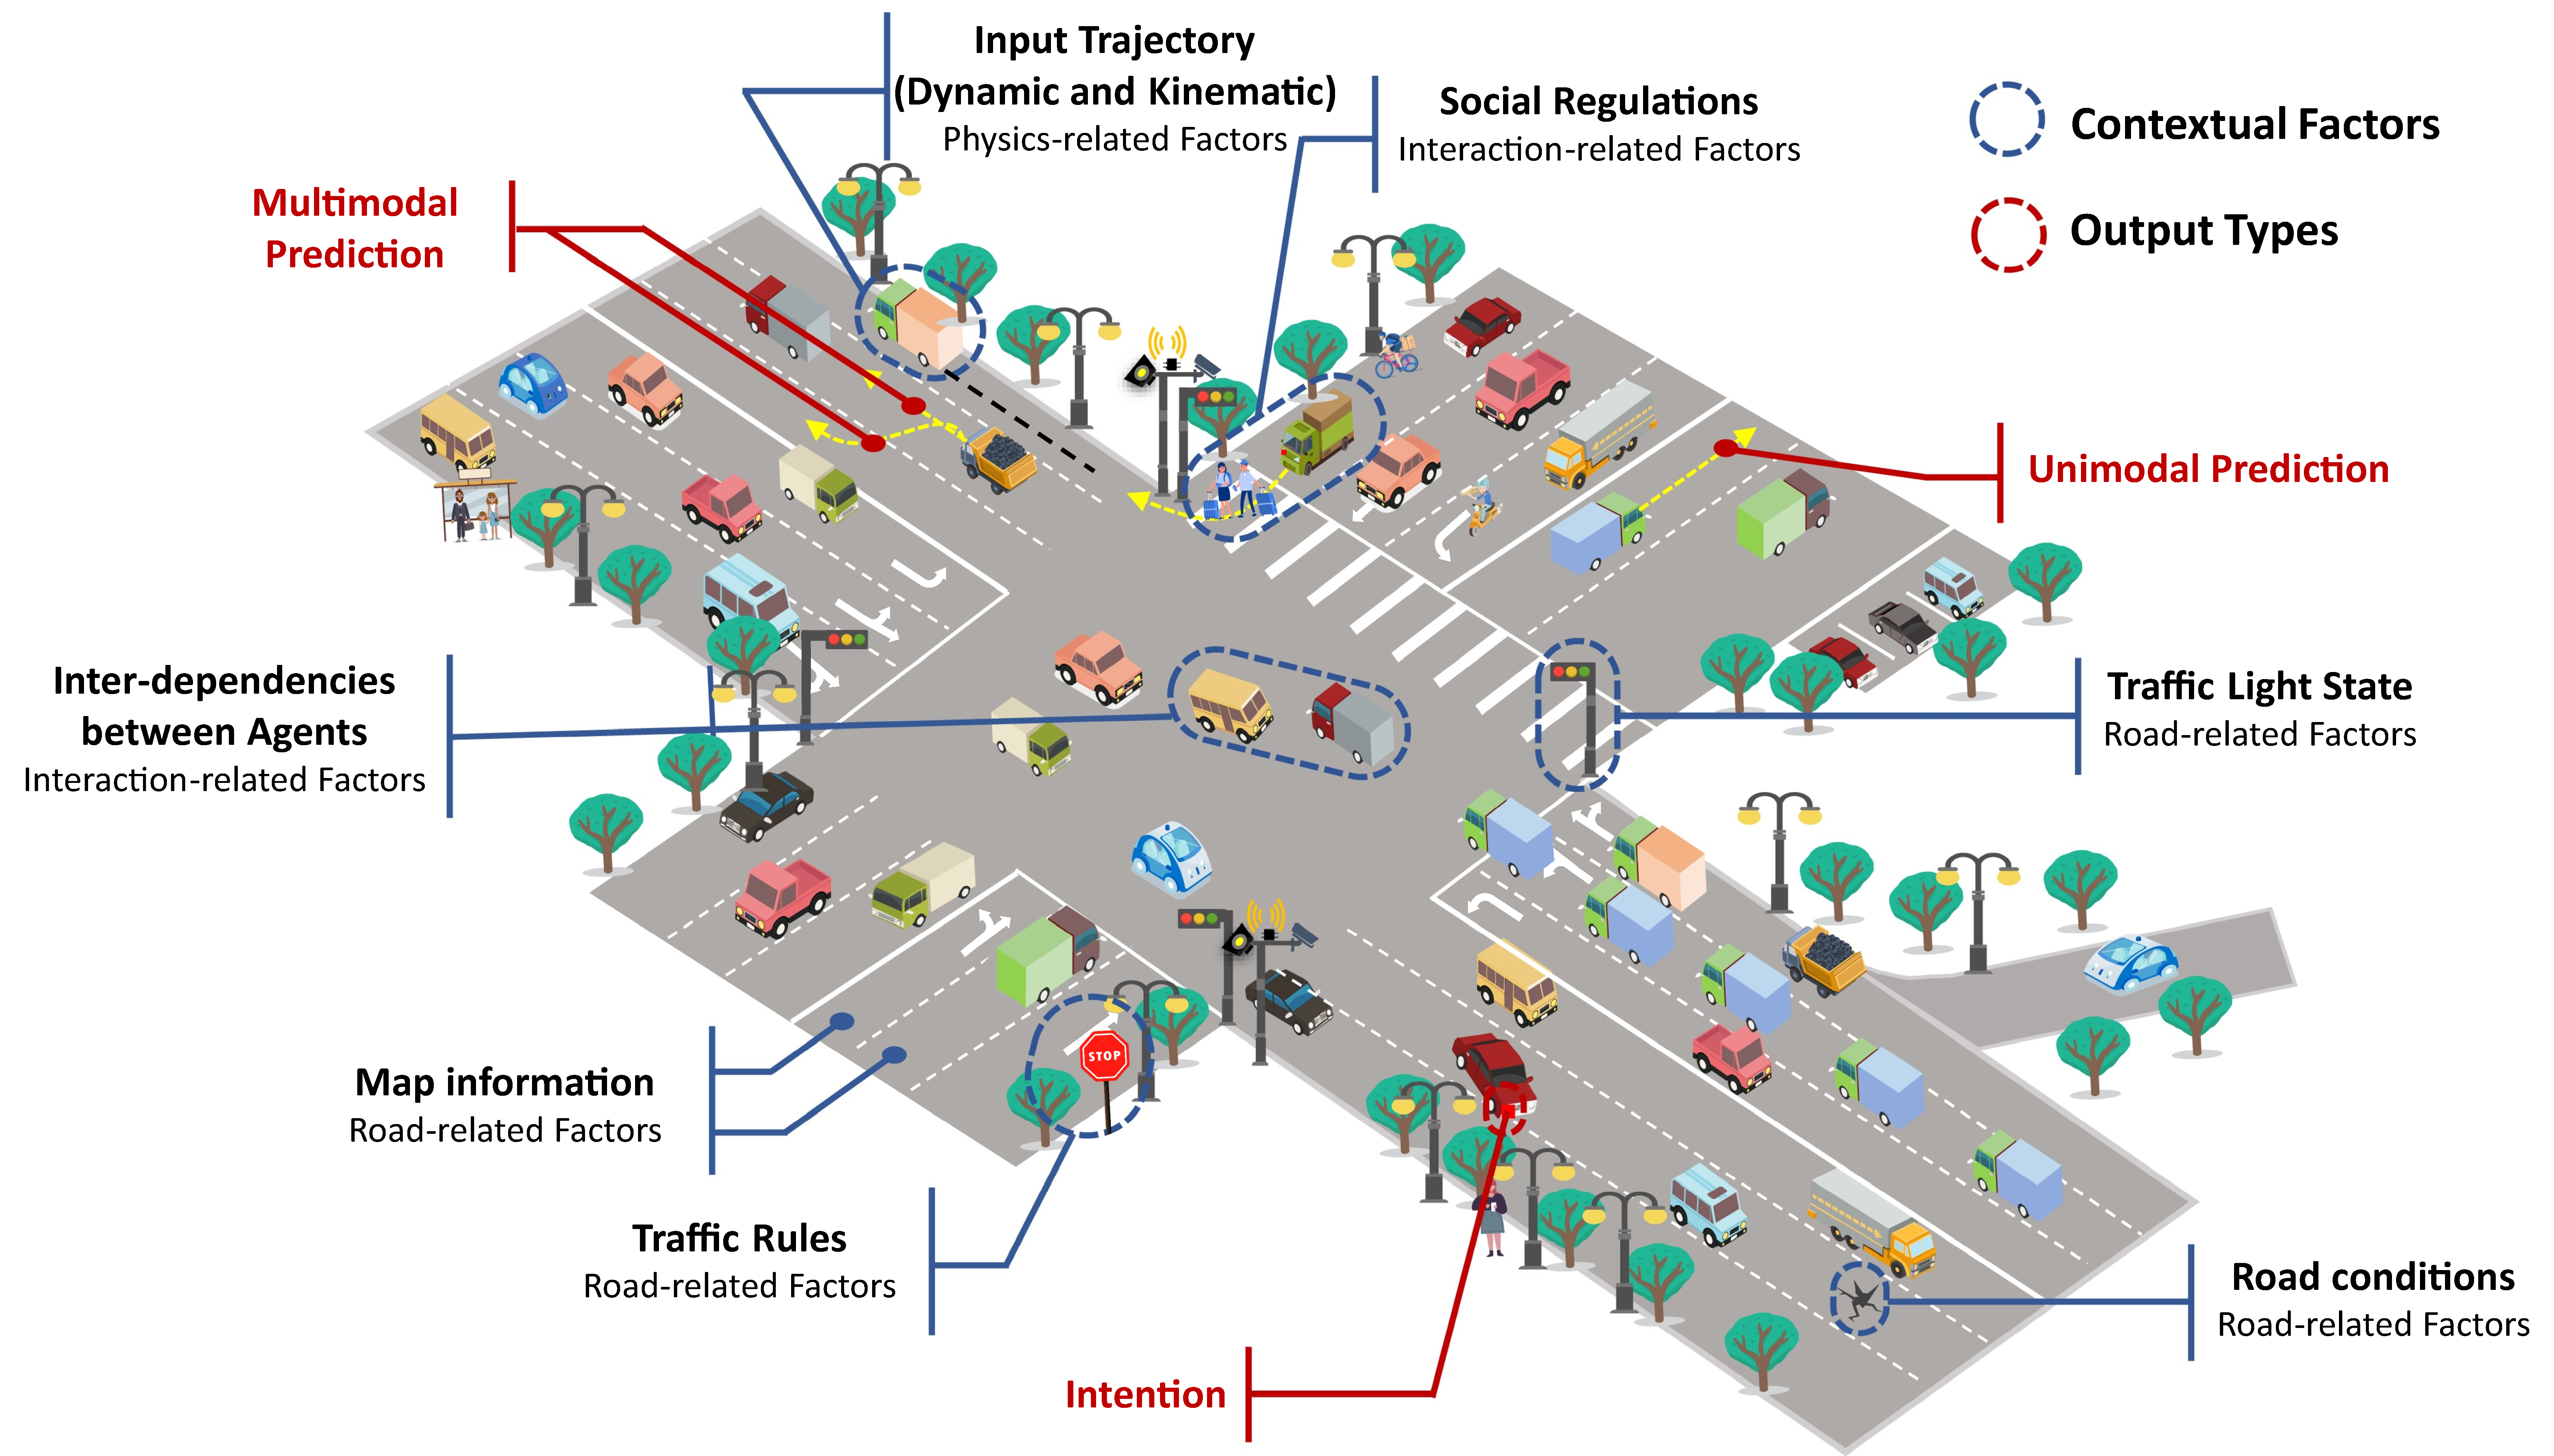
\includegraphics[width=\linewidth]{2_inputs_outputs_mp.pdf}
	\caption{Contextual factors and output types in Vehicle Motion Prediction}
	%Source: \textit{A survey on trajectory-prediction methods for autonomous driving} \cite{huang2022survey}
	\label{fig:2_input_output_map}
\end{figure}



\section{Problem Formulation of Motion Prediction}
\label{sec:2_problem_formulation_mp}

Given a sequence of past trajectories $a_{P}=[a_{-T^{'}+1},a_{-T^{'}+2},...,a_{0}]$ for an agent, we aim to predict its future steps $a_{F}=[a_{1},a_{2},...,a_{T}]$ up to a fixed time step $T$. Running in a specific traffic scenario, each actor will interact with static HD maps $m$ and the other dynamic actors, meeting the corresponding traffic and social rules. Therefore, the probabilistic distribution that we want to capture is $p(a_F|m, a_P, a^O_P)$, where $a^O_P$ denotes the other actors' observed states. 




The output of our model is $A_F = \{a_{F}^k\}_{k \in [0,K-1]}= \{(a_{1}^k,a_{2}^k,...,a_{T}^k)\}_{k \in [0,K-1]}$ for each actor, while motion forecasting tasks and subsequent decision modules usually expect us to output a set of trajectories. 
%
TNT \cite{zhao2020tnt}-like methods' distribution can be approximated as
\begin{equation}
	\sum_{\tau \in T(m, a_P, a^O_P)}{p(\tau|m, a_P, a^O_P)p(a_F|\tau, m, a_P, a^O_P)}
\end{equation}
where $T(m, a_P, a^O_P)$ is the space of candidate goals depending on the driving context.
However, the map space $m$ is large, and the goal space $T(m, a_P, a^O_P)$ requires careful design. In that sense, some methods expect to accurately predict the actor motion by extracting good features. For example, LaneGCN~\cite{liang2020learninggraph} tries to approximate $p(a_F|m, a_P, a^O_P)$ by modeling $p(a_F|M_{a_0}, a_P, a^O_P)$, where $M_{a_0}$ is a "local" map features that is related to the actor state $a_0$ at final observed step $t=0$. To extract $M_{a_0}$, they use $a_0$ as an anchor to retrieve its surrounding map elements and aggregate their features. As stated by \cite{wang2022ganet}, computing the local map information is only a part of the solution, but also proposing preliminary guidance for the model in a heuristic way, as well as calculating the goal area maps information using DL, may be of great importance for accuracy trajectory prediction. Then, our future probability distribution is enhanced by these preliminary preprocessed proposals and predicted goals as anchors to explicitly aggregate their surrounding map features as goal areas. 

\section{Physic-based Motion Prediction}
\label{sec:2_physic_based_mp}

\section{Deep Learning based Motion Prediction}
\label{sec:2_dl_based_mp}

\section{Vehicle Motion Prediction}
\label{sec:2_vehicle_based_mp}
%%%%%%%%%%%%%%%%%%%%%%%%%%%%%%%%%%%%%%%%%%%%%%%%%%%%%%%%%%%%%%%%%%%%%%%%%%% 
% 
% Generic template for TFC/TFM/TFG/Tesis
% 
% By:
% + Javier Macías-Guarasa. 
% Departamento de Electrónica
% Universidad de Alcalá
% + Roberto Barra-Chicote. 
% Departamento de Ingeniería Electrónica
% Universidad Politécnica de Madrid   
% 
% Based on original sources by Roberto Barra, Manuel Ocaña, Jesús Nuevo,
% Pedro Revenga, Fernando Herránz and Noelia Hernández. Thanks a lot to
% all of them, and to the many anonymous contributors found (thanks to
% google) that provided help in setting all this up.
% 
% See also the additionalContributors.txt file to check the name of
% additional contributors to this work.
% 
% If you think you can add pieces of relevant/useful examples,
% improvements, please contact us at (macias@depeca.uah.es)
% 
% You can freely use this template and please contribute with
% comments or suggestions!!!
% 
%%%%%%%%%%%%%%%%%%%%%%%%%%%%%%%%%%%%%%%%%%%%%%%%%%%%%%%%%%%%%%%%%%%%%%%%%%% 

\chapter{Theoretical Background}
\label{cha:theoretical_background}

\begin{FraseCelebre}
	\begin{Frase}
		Desde que el mundo cambió, \\
		estamos mucho más unidos con los Digimon, \\
		luchamos juntos contra el mal. \\ 

		Algo extraño pasaba, \\
		Digievolucionaban, en tamaño y color, \\
		Ellos son los Digimon. \\
	\end{Frase}
	\begin{Fuente}
		Opening 1 de Digimon: "Butterfly" \\
		Autor original: Kōji Wada
	\end{Fuente}
\end{FraseCelebre}

\section{Introduction}
\label{sec:3_introduction}

As commented in previous sections, the \ac{MP} algorithms covered by this thesis range from tracking multiple objects and subsequent prediction with physics-based methods to the most recent \ac{SOTA} techniques to compute the deep traffic context and then decode multimodal predictions with associated confidences, assuming the physical information is given and surrounding participants have been multi-tracked beforehand. Throughout this Chapter, an in-depth theoretical study will be made of those algorithms, neural networks or heuristics that form a direct part of the development of this work in order to address the proposed methods in future chapters.

First of all, we will start with the mathematical formulation of the methods to perform physics-based Multi-Object Tracking, from the well-known techniques Kalman Filter \cite{kalman1960new} for the agents states estimation to the Hungarian algorithm \cite{kuhn1955hungarian} for the association of detections and trackers, which represents the preliminary stage before carrying out the subsequent prediction. On top of that, since several single-trajectory models (\ac{CTRV}, \ac{CTRA}) are used to compute the most plausible centerlines in the Argoverse 1 \cite{chang2019argoverse} and Argoverse 2 \cite{wilson2023argoverse}, we will review the state transition equations to properly understand the constraints for each model. Furthermore, the principal \ac{DL} techniques (e.g. 1D-CNN, LSTM, GCN, Attention mechanisms) and training losses used in this work to encode and decode the aimed multimodal will be stated, first a general mathematical formulation and applications and then how the corresponding technique is used in the \ac{MP} field.

\section{Physics-based algorithms}
\label{sec:3_pb_formulation}

% https://arxiv.org/pdf/1710.04055.pdf
% https://github.com/NickNair/Multiple-Object-Tracking-using-Kalman-Filter

As stated in Chapter \ref{cha:related_works} Section \ref{sec:2_introduction}, initially researchers rely on physics-based methods which are basic and straightforward. These methods may not offer high accuracy, but many models use the underlying idea of physics-based models to improve their accuracy. Physics-based approaches yield better results when the movement of vehicles is described by kinematics or dynamics models accurately. Nevertheless, the physical model of traffic participants is constantly evolving, so most physics-based models are only applicable for short-term predictions of no more than one second. In this Section we will study the mathematical formulation of the physics-based prediction algorithms, as well as the data association problem regarding the Multi-Object Tracking stage, that are directly related to our algorithm proposed in Chapter \ref{cha:smartmot_exploiting_the_fusion_of_hdmaps_and_mot}.

\subsection{Kalman Filter under the hood}
\label{subsec:3_kf_formulation}

The Kalman Filter \cite{kalman1960new} is a recursive algorithm used for estimating the state of a dynamic system in the presence of noise. It is widely used in various fields such as engineering, control systems, and robotics. The algorithm works by combining a prediction of the system state based on a mathematical model with measurements (updates) from sensors to improve the accuracy of the state estimation, as shown in Figure \ref{fig:chapter_3_theoretical_background/KF_cycle}. The Kalman Filter is a powerful algorithm for state estimation, and it has many variations and extensions that can handle various types of systems and measurements. The filter can be applied to non-linear systems using the Extended Kalman Filter or the Unscented Kalman Filter, and it can handle multiple models using the multiple model Kalman Filter. The filter can also be used for smoothing, which involves estimating the state of the system based on past and future measurements.

\begin{figure}[h]
	\centering
	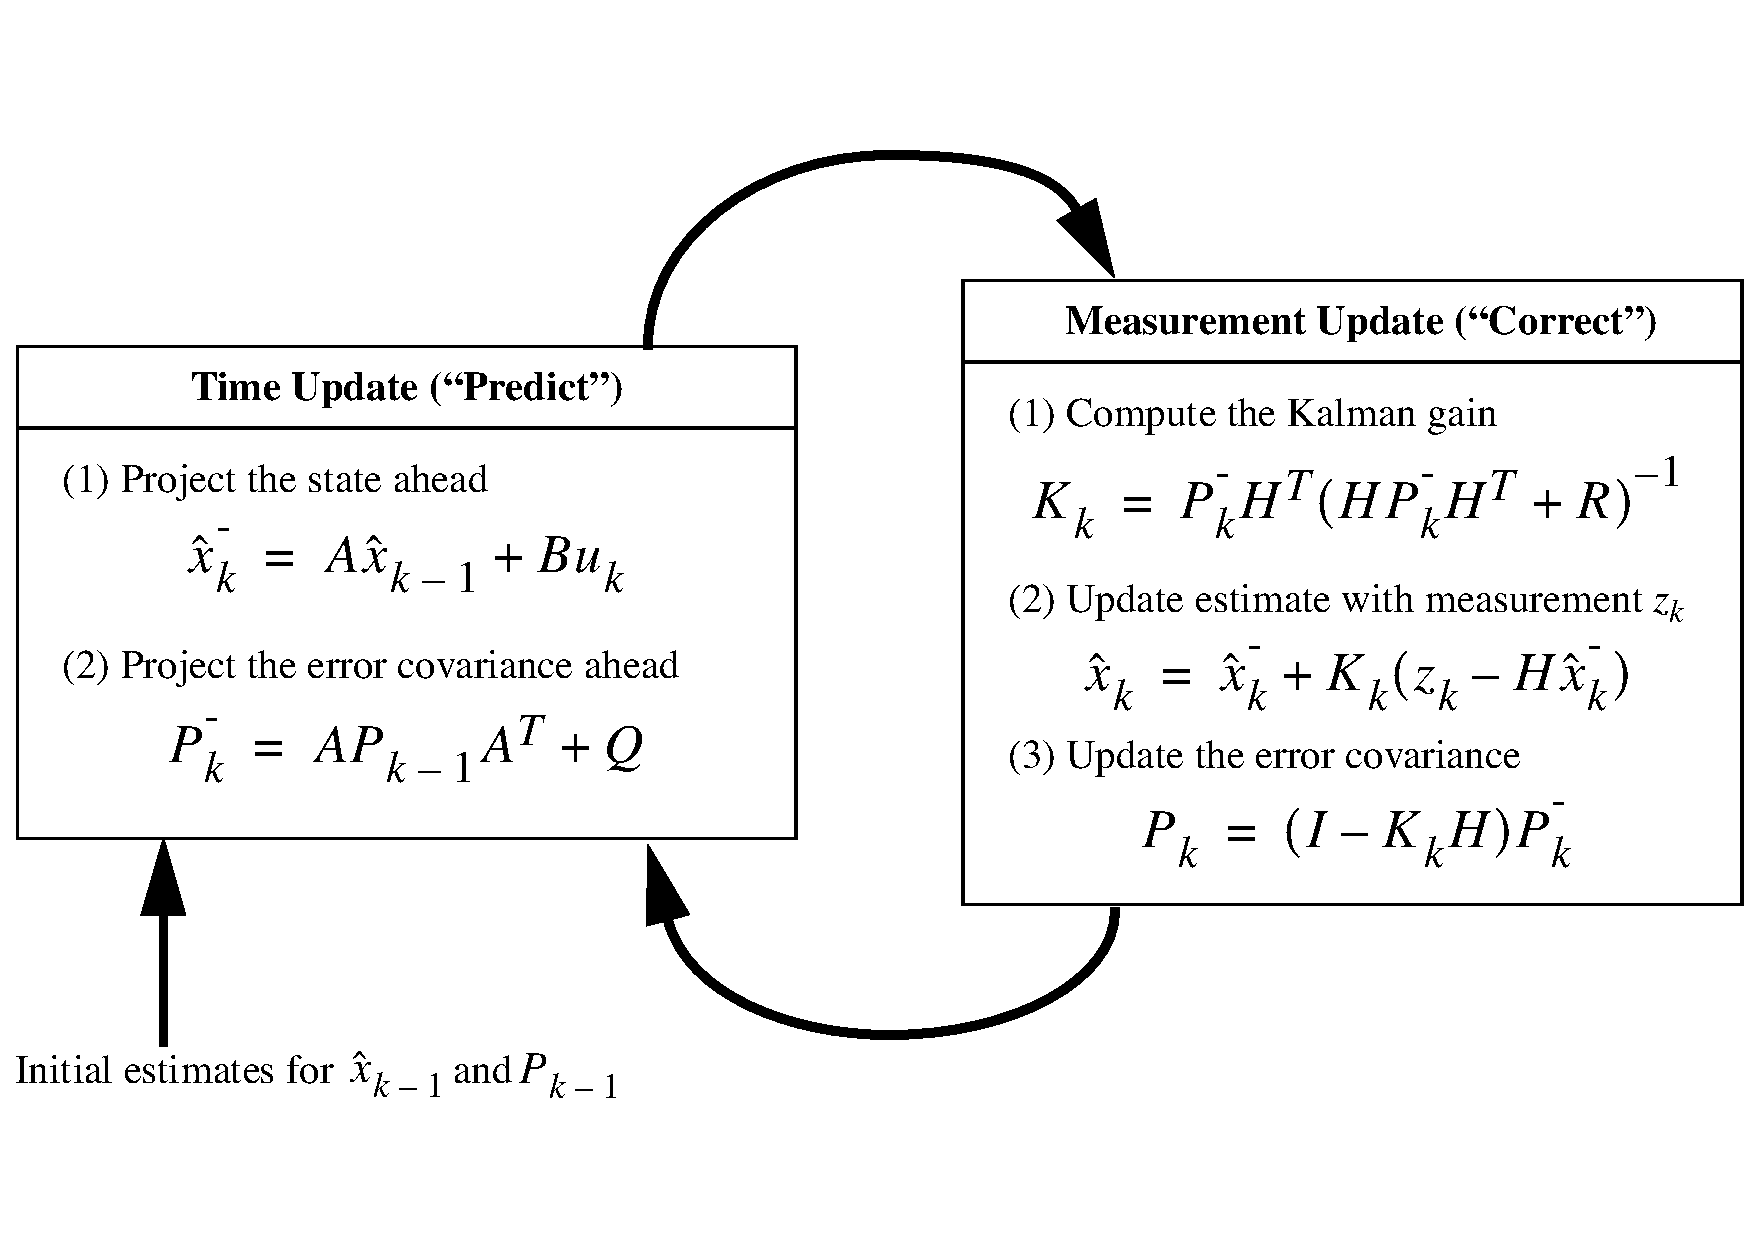
\includegraphics[width=\linewidth]{chapter_3_theoretical_background/KF_cycle.pdf}
	\caption[Overview of the Kalman Filter Predict-Update cycle]{Overview of the Kalman Filter Predict-Update cycle. The Kalman filter keeps track of the estimated state of the system and the variance or uncertainty of the estimate. The estimate is updated using a state transition model and measurements}
	Source: \textit{An introduction to the kalman filter} \cite{bishop2001introduction}
	\label{fig:chapter_3_theoretical_background/KF_cycle}
\end{figure}

In its most simple version, the Kalman filter assumes that the system can be described using a set of linear equations, where the state of the system can be represented by a vector $\mathbf{x}_k$, and the measurements can be represented by a vector $\mathbf{z}_k$. The Kalman filter also assumes that the noise in the system follows a Gaussian distribution.

The state estimation process is performed in two steps: the prediction step and the update step. In the prediction step, the current state of the system is predicted based on the previous state and a mathematical model of the system. In the update step, the predicted state is corrected based on a measurement from a sensor.

The prediction step can be represented using the following equations:

\begin{equation}
\begin{split}
	\hat{\mathbf{x}}_k^- = \mathbf{A} \hat{\mathbf{x}}_{k-1} + \mathbf{B} \mathbf{u}_k \\
	\mathbf{P}_k^- = \mathbf{A} \mathbf{P}_{k-1} \mathbf{A}^T + \mathbf{Q}
\end{split}
\end{equation}

where $\hat{\mathbf{x}}_k^-$ is the predicted state of the system at time $k$, $\hat{\mathbf{x}}_{k-1}$ is the estimated state of the system at time $k-1$, $\mathbf{A}$ is the state transition matrix, $\mathbf{B}$ is the control-input matrix, $\mathbf{u}_k$ is the control input at time $k$, $\mathbf{P}_k^-$ is the predicted error covariance matrix, and $\mathbf{Q}$ is the process noise covariance matrix. Note that the state transition, control-input and process noise covariance matrix values do not depend on the timestep time $k$.

On the other hand, the update step can be represented using the following equations:

\begin{equation}
	\begin{split}
		\mathbf{K}_k = \mathbf{P}_k^- \mathbf{H}_k^T (\mathbf{H} \mathbf{P}_k^- \mathbf{H}^T + \mathbf{R})^{-1} \\
		\hat{\mathbf{x}}_k = \hat{\mathbf{x}}_k^- + \mathbf{K}_k (\mathbf{z}_k - \mathbf{H}_k \hat{\mathbf{x}}_k^-) \\
		\mathbf{P}_k = (\mathbf{I} - \mathbf{K}_k \mathbf{H}) \mathbf{P}_k^-
	\end{split}
\end{equation}

where $\mathbf{K}_k$ is the Kalman gain, $\mathbf{H}$ is the measurement matrix, $\mathbf{R}_k$ is the measurement noise covariance matrix and $\mathbf{I}$ the identity matrix of the corresponding dimension. The Kalman gain determines the relative weight given to the predicted state and the measurement, and is adjusted based on the measurement noise covariance matrix. The measurement matrix relates the measurements to the state variables, and is used to convert the measurements into the same units as the state variables.

\subsection{Hungarian algorithm formulation}
\label{subsec:3_HA_formulation}

The Hungarian algorithm \cite{kuhn1955hungarian}, also known as the Munkres algorithm or the Kuhn-Munkres algorithm, is an efficient algorithm for solving the assignment problem in combinatorial optimization. The main concept behind this algorithm is an assignment problem that involves finding the optimal assignment of $n$ workers to $n$ jobs, given the cost of assigning each worker to each job.

The Hungarian algorithm works by iteratively finding a set of independent zero-cost assignments, which correspond to a perfect matching in a bipartite graph. These assignments are then used to reduce the problem size and find a new set of independent zero-cost assignments, until all workers are assigned to jobs.

The Hungarian algorithm has a time complexity of O($n^3$), which makes it one of the most efficient algorithms for solving the assignment problem. In this algorithm, the cost matrix C is assumed to be an $n \times n$ matrix, where each element $C_{i,j}$ represents the cost of assigning worker i to job j. The matrix M represents the matching, where each element $M_{i,j}$ is 1 if worker i is assigned to job j, and 0 otherwise.

\begin{algorithm}[]
	\SetAlgoLined
	\DontPrintSemicolon
	\SetKwInOut{Input}{Input}
	\SetKwInOut{Output}{Output}
	\Input{A cost matrix $C$ of size $n\times n$}
	\Output{A minimum cost perfect matching}
	Initialize the label vectors $u_i = \min_{j\in{1,\dots,n}} C_{i,j}$ and $v_j=0$ for all $i,j$;
	Initialize the empty matching $M$;
	\While{$|M| < n$}{
		Choose an unmatched row $i$;
		Initialize the set $T = {i}$ and the predecessor vector $P = \emptyset$;
		\While{true}{
			Let $S$ be the set of columns $j$ such that $i\in T$ and $C_{i,j} = u_i + v_j$;
			If $|S| > 0$, choose any column $j$ in $S$;
			\Else{
				Choose a column $j$ such that $v_j = \min_{k\in{1,\dots,n}} v_k$ and let $S$ be the set of rows $i$ such that $j\in M$ or $C_{i,j} = u_i + v_j$;
				Increment each $u_i$ for $i\in T$ by $\delta = \min_{i\in T,j\in S} (u_i+v_j-C_{i,j})$;
				Decrement each $v_j$ for $j\in S$ by $\delta$;
				\For{each row $i\in T$ and each column $j\in S$}{
					\If{$C_{i,j} = u_i+v_j$}{
						Add the edge $(i,j)$ to the alternating tree represented by $M$ and $P$;
						\If{$j$ is unmatched}{
							Augment $M$ along the alternating tree to create a larger matching;
							\Return the updated matching $M$;
						}
						\Else{
							Add $j$ to $T$ and continue the while loop;
						}
					}
				}
			}
		}
	}
	\caption{The Hungarian algorithm for solving the minimum cost perfect matching problem}
	\label{alg:3_ha}
\end{algorithm}

As observed in Algorithm \ref{alg:3_ha}, the Hungarian algorithm iteratively finds an uncovered zero in the cost matrix C and adds it to the matching M, while also adjusting the cost matrix to ensure that all rows and columns are covered by the matching. This is done by finding the minimum uncovered cost in each row and subtracting it from all uncovered costs in the row, and finding the minimum cost in each uncovered column and adding it to all uncovered costs in the column. Once all rows and columns are covered, the algorithm returns the final matching $M$.

In conclusion, the Hungarian algorithm is a powerful optimization algorithm that solves the assignment problem in polynomial time. The algorithm has a wide range of applications and can be easily adapted to handle various constraints and objectives. The algorithm is also guaranteed to find the optimal solution to the assignment problem, which makes it a valuable tool in many practical settings.
	
\subsection{State Transition Equations of Single-Trajectory Models}
\label{subsec:3_state_transitions_single_traj}

As stated in Chapter \ref{cha:related_works} Section \ref{subsubsec:2_single_trajectory_mp}, Single-trajectory prediction methods are used in the field of motion estimation and control, to predict the future state of an object based on its current state and motion. In these methods, the agents are mostly assumed to comply with motion models that describe their dynamic behavior in such a way these are not able to consider the road-related factors and the uncertainty of the current state is unreliable for long-term prediction. Then, these models should only be used for estimating unimodal trajectories of the surrounding agents in the short-term (no more than 1-s).

\begin{figure}[h]
	\centering
	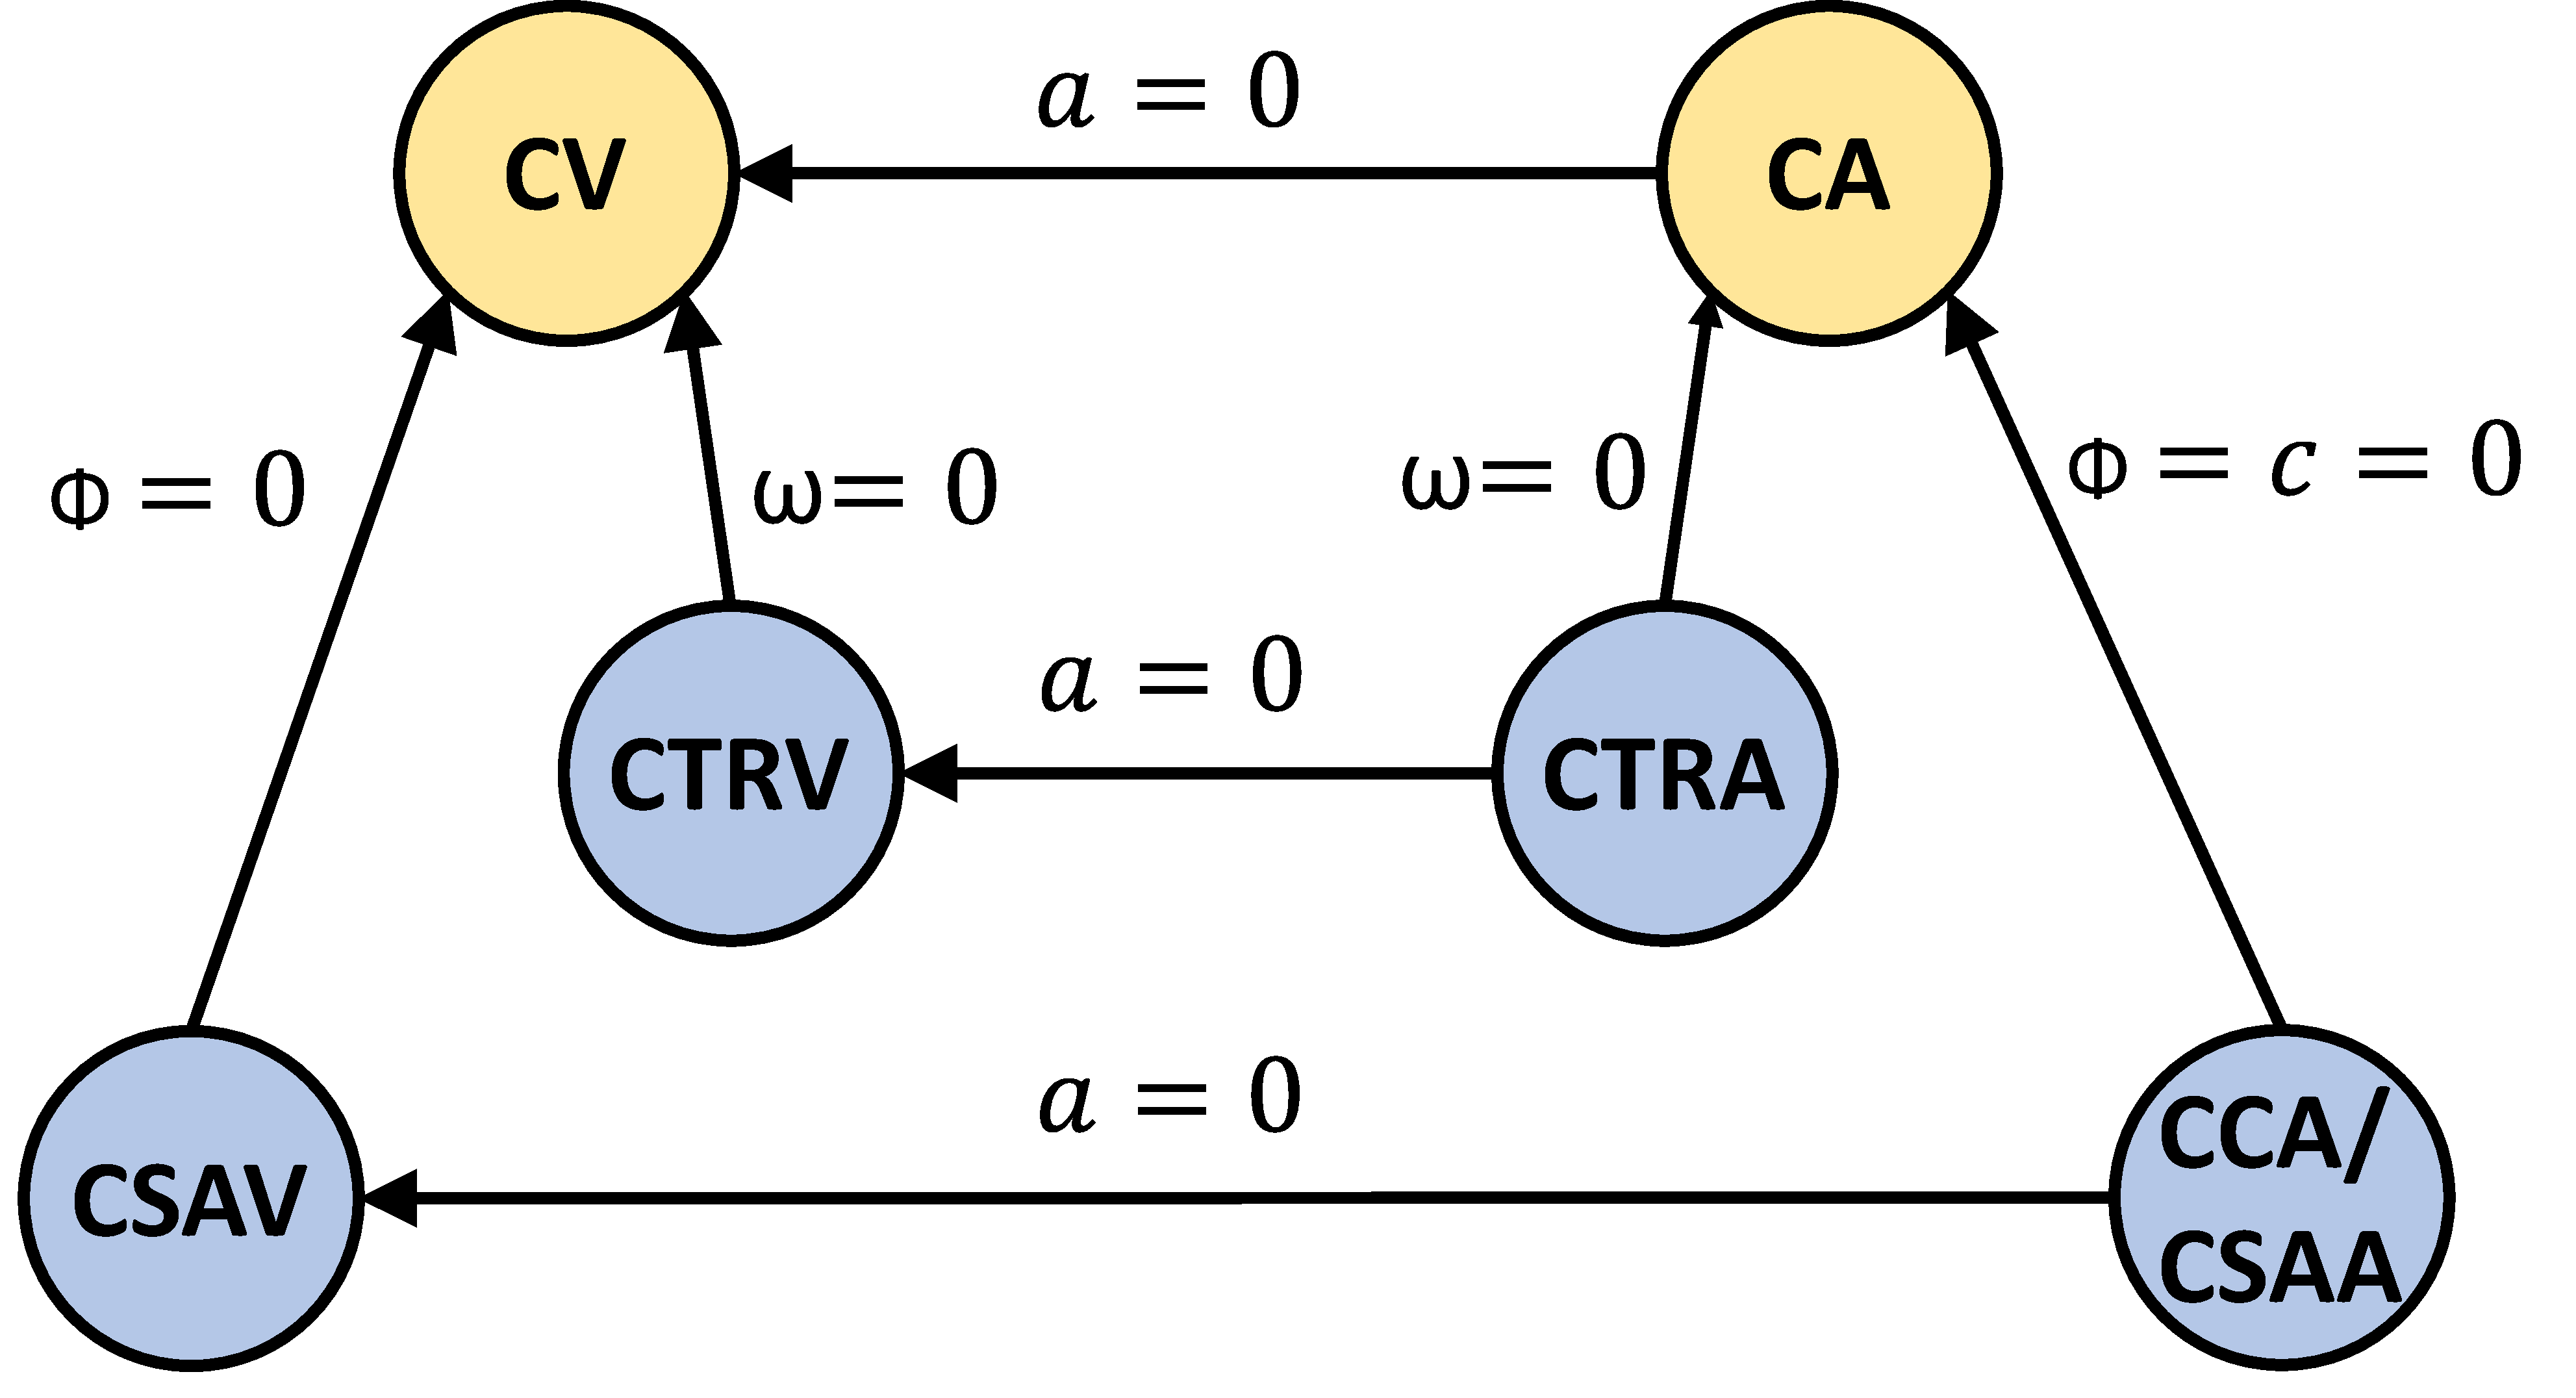
\includegraphics[width=0.6\linewidth]{chapter_3_theoretical_background/linear_curvilinear_mp.pdf}
	\caption[Overview of Single Trajectory prediction methods]{Overview of Single Trajectory prediction methods. Every sophisticated model can be transformed into a simpler one by setting one state veriable to zero}
	Source: \textit{Comparison and evaluation of advanced motion models for vehicle tracking} \cite{schubert2008comparison}
	\label{fig:chapter_3_theoretical_background/linear_curvilinear_mp}
\end{figure}

Several single-trajectory prediction models have been proposed in the literature, including Constant Velocity (CV), Constant Acceleration (CA), Constant Turn Rate and Velocity (CTRV), Constant Turn Rate and Acceleration (CTRA), Constant Speed and Angular Velocity (CSAV), and Constant Curvature Acceleration (CCA)/Constant Speed and Angular Acceleration (CSAA), as illustrated in Figure \ref{fig:chapter_3_theoretical_background/linear_curvilinear_mp}:

\begin{itemize}
	\item Constant Velocity (CV) model assumes that the object moves at a constant velocity and its future position can be predicted by simply extrapolating its current velocity vector. This model is simple and computationally efficient, but it may not accurately capture the object's motion if it changes its velocity.
	\item Constant Acceleration (CA) model is an extension of the CV model, assuming that the object can also change its acceleration in a linear manner. This model can provide more accurate predictions of the object's future position and velocity, but it may not be suitable for objects with more complex motion patterns.
	\item Constant Turn Rate and Velocity (CTRV) model assumes that the object moves in a circular trajectory with a constant turn rate and velocity magnitude. This model is useful for predicting the motion of objects such as drones or missiles, but it may not accurately represent the motion of objects with more complex trajectories.
	\item Constant Turn Rate and Acceleration (CTRA) model is an extension of the CTRV model, allowing the object to change its acceleration while maintaining a constant turn rate. This model is often used in applications such as autonomous driving or aircraft navigation, where objects can accelerate or decelerate.
	\item Constant Speed and Acceleration Vector (CSAV) model assumes that the object moves along a straight line with a constant speed and acceleration vector. This model can be useful for predicting the motion of objects such as trains or boats.
	\item Constant Acceleration and Angle (CAA) model assumes that the object moves along a constant heading angle and can change its acceleration in a linear manner. This model can be useful for predicting the motion of objects such as bicycles or motorcycles.
\end{itemize}

It can be observed how a sophisticated model can be transformed into a simpler one by setting one state veriable to zero. For example, CTRA is transformed to CTRV if the agent acceleration $a$ is set to zero. Similarly, CTRA is transformed to CA if the angular speed $\omega$ is set to 0. In this Section we particularly focus on the prediction equations and differences of the most commonly used single-trajectory prediction methods in the field of \ac{AD} to predict the future motion of a moving object: CTRV and CTRA.

\subsubsection{Constant Turn Rate Velocity (CTRV)}
\label{subsubsec:3_CTRV}

The Constant Turn Rate and Velocity (CTRV) model is a mathematical model used in the field of autonomous navigation to predict the future motion of a moving object. The model assumes that the object moves along a smooth, continuous path, and that its velocity and turn rate are constant.

The model describes the motion of the object using a set of differential equations that relate the rate of change of the object's state to its current state and any external inputs. The state of the object is described using five variables: the x and y coordinates of its position, its velocity magnitude, its heading angle (or direction of travel), and its turn rate.

The CTRV model predicts the future position of the object by using the current position, velocity, heading angle, and turn rate, and propagating them forward in time. The model assumes that the velocity and turn rate remain constant throughout the prediction interval.

The prediction equations for the CTRV model are described as follows:

\begin{equation}
\begin{split}
	x_{k+1} &= x_k + \frac{v_k}{\omega_k}\left[\sin(\psi_k+\omega_k\Delta t)-\sin(\psi_k)\right] \\
	y_{k+1} &= y_k + \frac{v_k}{\omega_k}\left[\cos(\psi_k)-\cos(\psi_k+\omega_k\Delta t)\right] \\
	v_{k+1} &= v_k \\
	\psi_{k+1} &= \psi_k + \omega_k\Delta t \\
	\omega_{k+1} &= \omega_k
\end{split}
\end{equation}
	
where:

$x_k$ and $y_k$ are the coordinates of the object's position at time step $k$
$v_k$ is the velocity magnitude at time step $k$
$\psi_k$ is the heading angle (in radians) at time step $k$
$\omega_k$ is the turn rate (in radians per second) at time step $k$
$\Delta t$ is the time step size.

The first two equations predict the object's position at the next time step, based on its current position, velocity, heading angle, and turn rate. The third and fifth equations predict that the velocity and turn rate will remain constant. The fourth equation predicts the object's heading angle at the next time step, based on its current heading angle and turn rate.

Overall, the CTRV model is a useful tool for predicting the motion of a moving object and can be used in a variety of applications, such as robotics, aviation, and space exploration.

\subsubsection{Constant Turn Rate Acceleration (CTRA)}
\label{subsubsec:3_CTRA}

The Constant Turn Rate and Acceleration (CTRA) model is an extension of the Constant Turn Rate and Velocity (CTRV) model, allowing the object to change its acceleration while maintaining a constant turn rate. This makes the CTRA model more accurate for predicting the motion of objects that can accelerate or decelerate, such as cars or aircraft.

The state of the object in the CTRA model is described using variables such as the x and y coordinates of its position, its velocity magnitude, its heading angle, its turn rate, and its acceleration magnitude. The motion of the object is modeled using the following set of equations:

\begin{equation}
\begin{split}
		x_{k+1} &= x_k + \frac{v_k}{\omega_k} \left[ \sin(\theta_k + \omega_k \Delta t) - \sin(\theta_k) \right] \\
		y_{k+1} &= y_k - \frac{v_k}{\omega_k} \left[ \cos(\theta_k + \omega_k \Delta t) - \cos(\theta_k) \right] \\
		\theta_{k+1} &= \theta_k + \omega_k \Delta t \\
		v_{k+1} &= v_k + a_k \Delta t \\
		\omega_{k+1} &= \omega_k
\end{split}
\end{equation}

where $x_k$ and $y_k$ are the object's position coordinates at time $k$, $\theta_k$ is its heading angle, $v_k$ is its velocity magnitude, $\omega_k$ is its turn rate, and $a_k$ is its acceleration magnitude. $\Delta t$ is the time step between predictions.

The first two equations describe the object's position updates based on its current position, velocity, heading angle, turn rate, and the time step. The third equation describes the object's heading angle update based on its current heading angle and turn rate. The fourth equation describes the object's velocity update based on its current velocity and acceleration. The last equation assumes that the object's turn rate remains constant over time.

In summary, the CTRA model is a useful tool for predicting the motion of objects that can accelerate or decelerate while maintaining a constant turn rate. The model's equations include variables such as the object's position, velocity, heading angle, turn rate, and acceleration magnitude, and they are based on the kinematic equations of motion.

\subsubsection{CTRV vs CTRA}
\label{subsubsec:3_CTRV_vs_CTRA}

The CTRV model assumes that the object moves along a smooth, continuous path, and that its velocity and turn rate are constant. This means that the object moves in a circular trajectory with a fixed radius. The state of the object is described using variables such as the x and y coordinates of its position, its velocity magnitude, its heading angle, and its turn rate.

On the other hand, the CTRA model assumes that the object can change its acceleration while maintaining a constant turn rate. This makes the CTRA model more accurate for predicting the motion of objects that can accelerate or decelerate, such as cars or aircraft. The state of the object in the CTRA model is described using similar variables to the CTRV model, but with an additional variable to represent the object's acceleration.

The prediction equations for the CTRV model are based on the kinematic equations for circular motion, where the object's position, velocity, and heading angle change in a continuous and smooth manner. In contrast, the prediction equations for the CTRA model include an additional term for the object's acceleration, which allows for more accurate predictions of the object's future motion when it can accelerate or decelerate.

In terms of implementation, the CTRA model requires more computational resources due to the additional term for acceleration, which increases the complexity of the equations. This can make the CTRV model more computationally efficient and faster to calculate in real-time applications. However, the CTRA model is more accurate in predicting the motion of objects with varying acceleration and is often used in applications such as autonomous driving or aircraft navigation.

In summary, the main differences between the CTRV and CTRA prediction models are that the CTRA model includes an additional term for acceleration in its prediction equations, allowing for more accurate predictions of the motion of objects with varying acceleration, while the CTRV model assumes a constant velocity and turn rate and is more computationally efficient.

\section{Deep Learning algorithms}
\label{sec:3_dlb_formulation}

In this section the mathematical formulation of the \ac{DL} layers employed in this thesis is covered. In particular, these are the 1D-\ac{CNN}, \ac{LSTM}, \ac{GAN}, Attention mechanism and \ac{GNN} layers. We briefly introduce each layer, as well as the corresponding mathematical formulation to enhance the comprehension of the learning-based methods proposed in this thesis.

\subsection{Convolutional Neural Networks}
\label{subsec:3_cnns}

% Additional info

% https://towardsdatascience.com/understanding-1d-and-3d-convolution-neural-network-keras-9d8f76e29610
% file:///C:/Users/Carlos/Downloads/sensors-22-09517.pdf
% https://e2eml.school/convolution_one_d.html
% https://arxiv.org/pdf/1512.07108.pdf

Convolutional neural networks (CNNs) are commonly used for image and signal processing tasks. The type of CNN architecture used depends on the nature of the input data. Here are the differences between the three types of CNNs:

\begin{itemize}
	\item 1D Convolutional Neural Networks (1D CNNs): 1D CNNs are used for processing sequential data such as time series data, speech signals, and text data. The input to a 1D CNN is a one-dimensional sequence of data, such as a time series of sensor readings. 1D CNNs typically have fewer parameters and are computationally efficient compared to 2D and 3D CNNs.
	
	\item 2D Convolutional Neural Networks (2D CNNs): 2D CNNs are used for processing 2D images. The input to a 2D CNN is a two-dimensional image represented as a matrix of pixels. The convolutional layers in a 2D CNN apply filters that slide over the image to extract local features. The output of each convolutional layer is a set of 2D feature maps. 2D CNNs are widely used for image classification, object detection, and image segmentation.
	
	\item 3D Convolutional Neural Networks (3D CNNs): 3D CNNs are used for processing 3D volumetric data such as CT scans, MRI images, and video data. The input to a 3D CNN is a three-dimensional volume represented as a sequence of 2D images. The convolutional layers in a 3D CNN apply filters that slide over the 3D volume to extract local features. The output of each convolutional layer is a set of 3D feature maps. 3D CNNs are used for tasks such as medical image analysis, video classification, and action recognition.
\end{itemize}

In summary, 1D CNNs are used for processing sequential data (such as time series data, audio signals, and text), 2D CNNs are used for image processing, and 3D CNNs are used for volumetric data. As we will see in Chapter \ref{cha:predictive_techniques_in_ad}, in this work we focus on 1D CNNs. The basic building blocks of a 1D CNN are convolutional layers, which learn local patterns in the input data by applying a set of filters to it, as illustrated in Figure \ref{fig:chapter_3_theoretical_background/CNN_1D}. Each filter slides over the input sequence and performs a dot product operation at each position to generate a feature map. These feature maps capture the presence of certain patterns at different positions in the input sequence. 
 
The architecture of a 1D CNN typically consists of several convolutional layers, followed by one or more fully connected layers for classification or regression. The output of each convolutional layer is fed into the next layer, with optional pooling layers in between to reduce the spatial dimension of the feature maps. The final output of the network is obtained by passing the output of the last fully connected layer through a suitable activation function, such as softmax for classification or linear for regression.
 
 \begin{figure}[h]
 	\centering
 	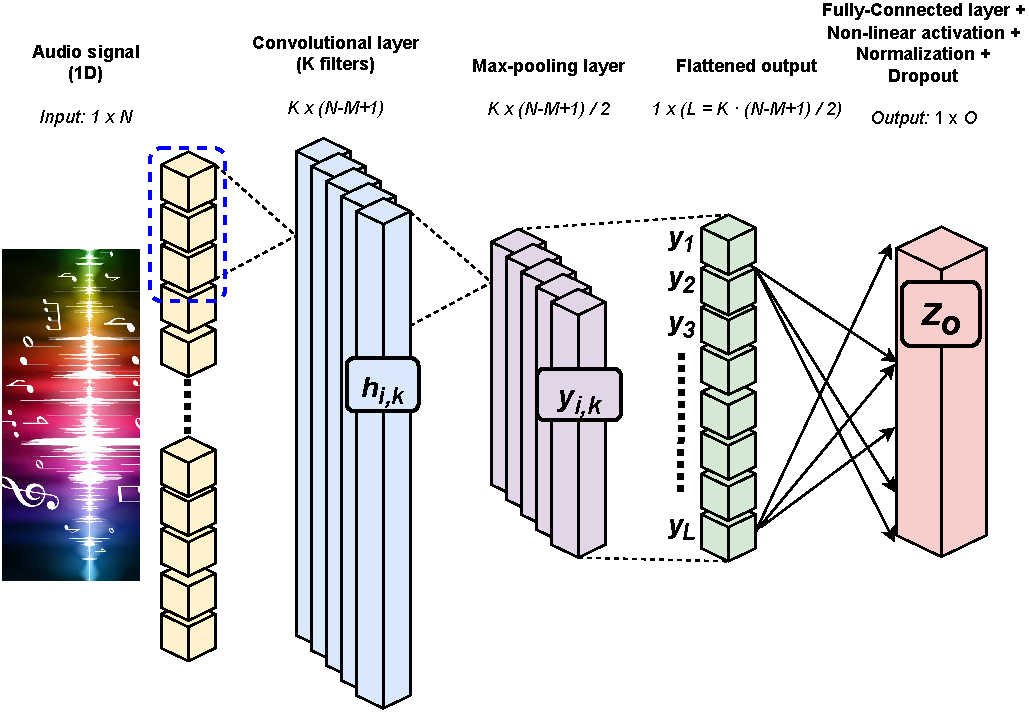
\includegraphics[width=0.6\linewidth]{chapter_3_theoretical_background/CNN_1D.pdf}
 	\caption{Example of CNN architecture to process 1D-input signals}
 	\label{fig:chapter_3_theoretical_background/CNN_1D}
 \end{figure}
 
Let $x$ be a 1-dimensional input sequence of length $n$, represented as a vector $x = [x_1, x_2, ..., x_n]$. Let $k$ be a filter of length $m$, represented as a vector $k = [k_1, k_2, ..., k_m]$. We can apply the filter $k$ to the input sequence $x$ by computing a convolution operation:

\begin{equation}
	(k * x)_i = \sum_{j=1}^m k_j x_{i+j-m}
\end{equation}

where $*$ denotes the convolution operation, and $i$ ranges from $m$ to $n$. This operation produces a new sequence of length $n - m + 1$, representing the local features extracted from the input sequence $x$ by the filter $k$.

To learn multiple filters and extract different types of features, we use multiple convolutional layers in the network. Each layer applies a set of filters, and produces a set of feature maps. The feature maps can be computed as:

\begin{equation}
h_{i,j} = f(\sum_{k=1}^m W_{j,k} x_{i+k-m} + b_j)
\end{equation}

where $h$ is the feature map at position $i$ and filter $j$, $W$ is the weight matrix of the $j$-th filter, $b$ is the bias term for the $j$-th filter, and $f$ is an activation function (such as ReLU or sigmoid).

After each convolutional layer, we typically apply a pooling layer to reduce the dimensionality of the features and increase the translation invariance of the network. The most common pooling operation is max pooling, which selects the maximum value within a window of size $p$:

\begin{equation}
y_{i,j} = \max_{k=0}^{p-1} h_{i+k,j}
\end{equation}

where $y$ is the output of the pooling layer at position $i$ and filter $j$.

Finally, we can use one or more fully connected layers to perform the final classification or regression task. The output of the pooling layer is flattened into a vector, and fed into a set of fully connected layers, with optional dropout regularization and batch normalization:

\begin{equation}
z_j = f(\sum_{i=1}^n W_{i,j} y_i + b_j)
\end{equation}

where $z$ is the output of the $j$-th fully connected layer, $W$ is the weight matrix, $y$ is the flattened output of the pooling layer, $b$ is the bias term, and $f$ is an activation function. 

\subsection{Recurrent Neural Networks}
\label{subsec:3_rnns}

Recurrent Neural Networks (RNNs) are a type of neural network that are designed to process sequential data, where the order of the input matters. They are widely used in a variety of applications such as natural language processing, speech recognition, image captioning, and time series prediction.

The general theory of RNNs is that they have a feedback loop in their architecture that allows information to be passed from one time step to the next, thereby enabling the network to capture dependencies between the inputs at different time steps. The input at each time step is fed into the network along with the output from the previous time step, and the network uses this information to generate a new output.

There are several types of RNNs, including the basic RNN, the Gated Recurrent Unit (GRU), and the Long Short-Term Memory (LSTM) \cite{hochreiter1997long}. The basic RNN is the simplest form of RNN, where the output at each time step is a function of the input at that time step and the output from the previous time step. However, it suffers from the vanishing gradient problem, where the gradients become exponentially small as they propagate through time, making it difficult to learn long-term dependencies.

The GRU is a variation of the basic RNN that uses gating mechanisms to control the flow of information through the network. It has fewer parameters than the LSTM and can be faster to train, but it may not perform as well as the LSTM on tasks that require more complex temporal dependencies.

\subsubsection{Long Short-Term Memory}
\label{subsubsec:3_LSTMs}

LSTM networks were introduced to address the vanishing gradient problem in standard RNNs. They achieve this by using a memory cell to store information over long periods of time, and three gating mechanisms to control the flow of information through the network. Figure \ref{fig:chapter_3_theoretical_background/LSTM} provides a detailed overview of the LSTM cell structure, illustrating the workflow from the previous cell output and input at time $t-1$ in order to compute the current cell state and hidden state at time $t$.

\begin{figure}[h]
	\centering
	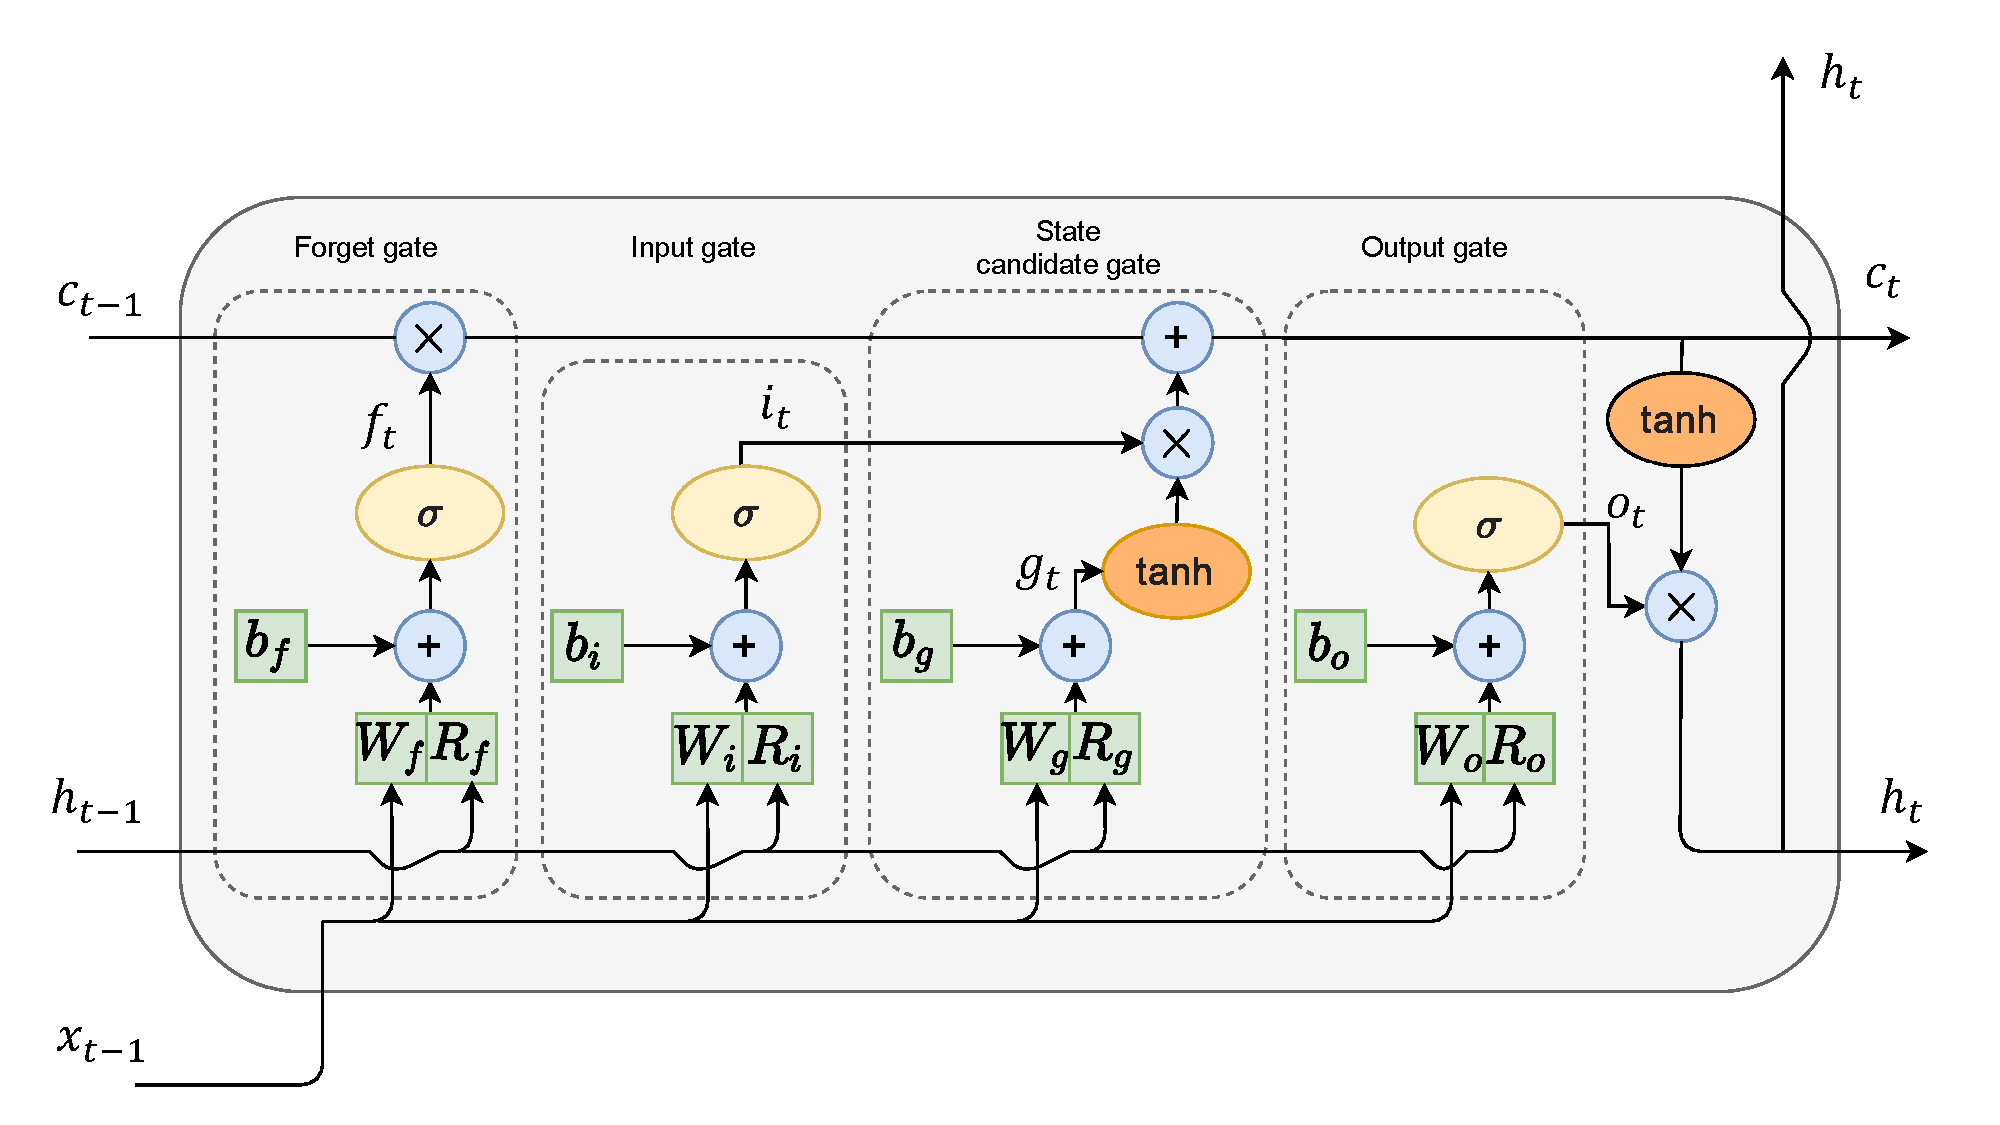
\includegraphics[width=\linewidth]{chapter_3_theoretical_background/LSTM_cell.pdf}
	\caption{Overview of the LSTM cell structure}
	\label{fig:chapter_3_theoretical_background/LSTM}
\end{figure}

The three gates are called the input gate, forget gate, and output gate, and they are responsible for deciding which information to store in the memory cell, which information to forget, and which information to output, respectively.

The equations for the input, forget, and output gates are as follows:

\begin{itemize}
	\item Input gate: $i_t = \sigma(W_i \cdot [h_{t-1}, x_t] + b_i)$
	\item Forget gate: $f_t = sigmoid(W_f * [h_{t-1}, x_t] + b_f)$
	\item Input gate: $o_t = sigmoid(W_o * [h_{t-1}, x_t] + b_o)$
\end{itemize}

where $x_t$ is the input at time $t$, $h_{t-1}$ is the hidden state from the previous time step, $i_t$ is the input gate activation, $f_t$ is the forget gate activation, and $o_t$ is the output gate activation. $W_i$, $W_f$, and $W_o$ are weight matrices, and $b_i$, $b_f$, and $b_o$ are bias vectors.

On the other hand, the memory cell is updated based on the input, forget, and output gates, as well as a new candidate value that is computed based on the current input and hidden state. The equations for the memory cell and candidate value are as follows:

\begin{equation}
\begin{split}
		\tilde{C}t &= \tanh(W_c \cdot [h{t-1}, x_t] + b_c) \\
		C_t &= f_t \cdot C_{t-1} + i_t \cdot \tilde{C}_t 
\end{split}
\end{equation}

where $\tilde{C}t$ is the candidate value, $C_t$ is the new memory cell value, and $C{t-1}$ is the previous memory cell value. $W_c$ is a weight matrix and $b_c$ is a bias vector.

Finally, the hidden state at time $t$ is computed based on the output gate and the new memory cell value, using the following equation:

\begin{equation}
	h_t = o_t \cdot \tanh(C_t)
\end{equation}

This equation scales the memory cell value by the output gate activation, then applies a hyperbolic tangent function to obtain the new hidden state.

In summary, LSTMs use a memory cell and three gating mechanisms to learn long-term dependencies in sequential data. The input, forget, and output gates control the flow of information through the network, while the memory cell stores information over time. The equations for LSTMs involve computing the input, forget, and output gate activations, the candidate value, the new memory cell value, and the new hidden state.

\subsection{Generative Adversarial Networks}
\label{subsec:3_gans}

A discriminative model is a type of machine learning model that learns the relationship between the input features and the target output directly. The goal of a discriminative model is to learn a decision boundary that separates different classes in the input data. In other words, discriminative models focus on learning the conditional probability distribution of the target variable given the input features.

Discriminative models are often used in supervised learning tasks, such as classification and regression, where the goal is to predict a target variable based on a set of input features. Common examples of discriminative models include logistic regression, support vector machines, and neural networks.

Unlike generative models, which learn the joint probability distribution of the input and target variables, discriminative models do not model the probability distribution of the input data explicitly. Instead, they focus on learning a mapping function that directly maps the input features to the target output.

In 2014, a breakthrough paper introduced Generative adversarial networks (GANs) \cite{goodfellow2020generative}, a clever new way to leverage the power of discriminative models to get good generative models. At their heart, GANs rely on the idea that a data generator is good if we cannot tell fake data apart from real data. In statistics, this is called a two-sample test - a test to answer the question whether datasets $X=\{x_1,\ldots, x_n\}$ and $X'=\{x'_1,\ldots, x'_n\}$ were drawn from the same distribution. This allows to improve the data generator until it generates something that resembles the real data. At the very least, it needs to fool the classifier even if our classifier is a state of the art deep neural network. GANs are a powerful technique for generating realistic samples that are similar to some training data. A GAN consists of two neural networks, a generator network and a discriminator network. The generator and discriminator networks are trained in a two-player game, where the generator tries to produce samples that fool the discriminator, and the discriminator tries to correctly classify between real and generated data. The objective function for a GAN is a min-max game between the generator and discriminator, and can be optimized using gradient descent or some other optimization algorithm. Some common applications where GANs are widely used are generating realistic images, videos, audio, data augmentation or style transfer.

The generator network takes as input a random noise vector, and generates a sample that is meant to mimic real data. The discriminator network takes as input a sample, and tries to distinguish between real data and generated data. The two networks are trained in a two-player game, where the generator tries to produce samples that fool the discriminator, and the discriminator tries to correctly classify between real and generated data.

The objective function for a GAN can be formulated as a min-max game between the generator and discriminator. The generator tries to minimize the probability that the discriminator correctly classifies the generated samples as fake, while the discriminator tries to maximize the probability that it correctly classifies the real and generated samples.

The objective function for a GAN can be written as:

\begin{equation}
\begin{split}
	\min_{\theta_G}\max_{\theta_D} V(D, G) = \mathbb{E}{x\sim p{data}(x)}[\log D(x)] + \mathbb{E}{z\sim p_z(z)}[\log(1-D(G(z)))] \\
	= \mathbb{E}{x\sim p_{data}(x)}[\log D(x)] + \mathbb{E}_{z\sim p_z(z)}[\log(1-D(G(z;\theta_G)))]
\end{split}
\end{equation}

where $\theta_G$ and $\theta_D$ are the parameters of the generator and discriminator networks, respectively, $x$ is a real sample from the training data distribution $p_{data}$, $z$ is a noise vector sampled from a prior distribution $p_z$, and $G(z;\theta_G)$ is the generated sample from the generator network.

The first term of the objective function represents the expected log-probability of the discriminator correctly classifying a real sample as real. The second term represents the expected log-probability of the discriminator correctly classifying a generated sample as fake.

During training, the generator network is updated to minimize the objective function with respect to $\theta_G$, while the discriminator network is updated to maximize the objective function with respect to $\theta_D$. This can be done using gradient descent or some other optimization algorithm.

There are some well-known types of GANs, such as:

\begin{itemize}
	\item Deep Convolutional GANs (DCGANs): These are GANs that use convolutional neural networks (CNNs) in the generator and discriminator networks. DCGANs are commonly used for image generation and have been shown to produce high-quality, realistic images.
	\item Wasserstein GANs (WGANs): These are GANs that use the Wasserstein distance instead of the traditional Kullback-Leibler (KL) divergence or Jensen-Shannon (JS) divergence for measuring the difference between the real and generated distributions. WGANs have been shown to produce more stable training and generate higher-quality samples.
	\item CycleGANs: These are GANs that are designed for image-to-image translation tasks, where the goal is to transform an image from one domain to another. CycleGANs use two generators and two discriminators to learn the mapping between the two domains.
\end{itemize}

Nevertheless, in this work we focus on a particular type of GAN, known as conditional GAN or cGAN, where the generator is conditioned on some additional information, such as class labels or image annotations. The additional information is used to control the generated output, allowing for more specific generation of data. 

\subsubsection{GAN vs cGAN}
\label{subsubsec:3_cGAN}

The main difference between the original GAN and cGAN is that the original GAN generates samples without any control over the generated output, whereas the cGAN generates samples conditioned on some additional information.

In the original GAN, the generator network takes as input a random noise vector, and generates a sample that is meant to mimic real data. The discriminator network takes as input a sample, and tries to distinguish between real data and generated data. The goal of the original GAN is to train the generator network to generate samples that are indistinguishable from real data.

\begin{figure}[h]
	\centering
	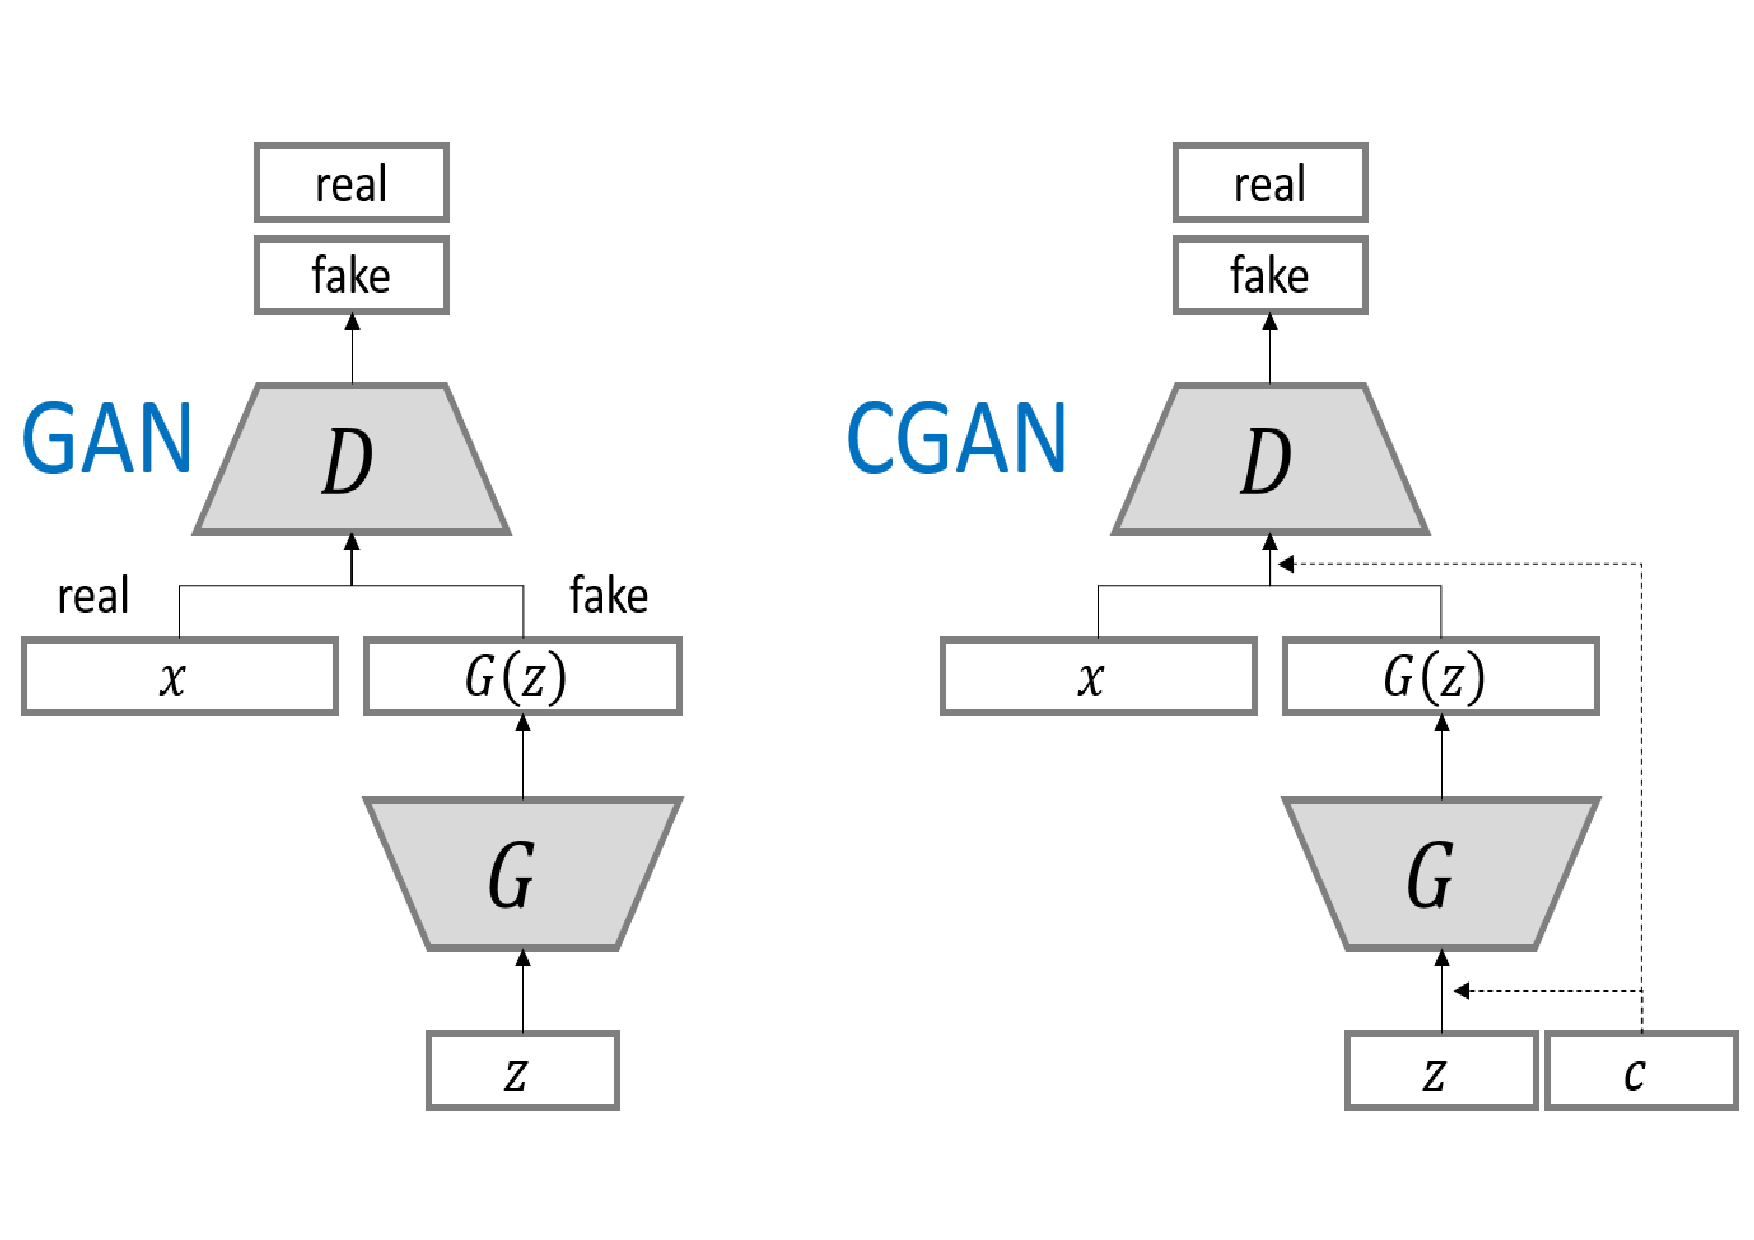
\includegraphics[width=0.5\linewidth]{chapter_3_theoretical_background/GAN.pdf}
	\caption{Comparison between the original Generative Adversarial Network (GAN) and conditional GAN (cGAN)}
	\label{fig:chapter_3_theoretical_background/GAN}
\end{figure}

In contrast, a cGAN is a GAN that is conditioned on some additional information, such as class labels or image annotations. The generator network in a cGAN takes as input both a random noise vector and a condition vector, and generates a sample that is conditioned on the additional information. The discriminator network also takes as input both the sample and the condition vector, and tries to distinguish between real data and generated data based on the condition. Figure \ref{fig:chapter_3_theoretical_background/GAN} illustrates the differences between the original GAN and the corresponding conditioned architecture.

The cGAN can be used for a variety of applications, such as image-to-image translation, where the additional information is an input image that is translated to a different output image. For example, a cGAN can be trained to convert grayscale images to color images, or to transform images of one type of object to another type of object.

The training process for a cGAN is similar to that of the original GAN, but the loss function for the generator and discriminator networks are modified to include the condition vector. Specifically, the loss function for the generator network includes a term that measures how well the generated samples match the condition vector, in addition to the term that measures how well the generated samples fool the discriminator. Similarly, the loss function for the discriminator network includes a term that measures how well the discriminator can identify the condition vector, in addition to the term that measures how well it can distinguish between real and generated data.

The cGAN can be used for a variety of applications, such as image-to-image translation, where the additional information is an input image that is translated to a different output image. For example, a cGAN can be trained to convert grayscale images to color images, or to transform images of one type of object to another type of object.

\subsection{Attention Mechanism}
\label{subsec:3_attention}

The attention mechanism is a computational method used in deep learning models to help the model focus on the most important parts of the input data. It is commonly used in natural language processing, speech recognition, and computer vision.

The basic idea of attention is to compute a set of weights that indicate the relative importance of different parts of the input. These weights are then used to compute a weighted sum of the input, which is used as the output of the attention mechanism.

The attention mechanism can be formulated mathematically using the following equations:

First, we compute a set of "keys", "values", and a "query" vector, which are used to compute the attention weights:

\begin{equation}
\begin{split}
	K = {k_1, k_2, ..., k_n}
	V = {v_1, v_2, ..., v_n}
	q = [q_1, q_2, ..., q_d]
\end{split}
\end{equation}

where $n$ is the number of elements in the input, and $d$ is the dimension of the query vector. Next, we compute the attention weights using a function that compares the query vector to each of the keys:

\begin{equation}
	a_i = \text{softmax}(q^T k_i)
\end{equation}

where $a_i$ is the attention weight for the $i$th element of the input. Finally, we compute the output of the attention mechanism as a weighted sum of the values:

\begin{equation}
	o = \sum_{i=1}^{n} a_i v_i
\end{equation}

\subsubsection{Positional Encoding}
\label{subsubsec:3_positional_encoding}

In the attention mechanism, positional encoding is used to incorporate the order of the input sequence into the model. Positional encoding involves adding a fixed-length vector to the input embeddings that encodes the position of each element in the sequence.

The mathematical formulation of positional encoding is as follows:

\begin{equation}
	\text{PE}_{(pos,2i)} = \sin\left(\frac{pos}{10000^{2i/d}}\right)
\end{equation}

\begin{equation}
	\text{PE}_{(pos,2i+1)} = \cos\left(\frac{pos}{10000^{2i/d}}\right)
\end{equation}

where $pos$ is the position of the element in the sequence, $i$ is the index of the dimension, and $d$ is the dimension of the input embeddings. The positional encoding vectors are added to the input embeddings before they are passed through the self-attention mechanism.

The choice of the constants used in the positional encoding formulation, such as the use of the sine and cosine functions and the value of $10000$, is arbitrary but has been shown to work well in practice. The positional encoding vectors add a sinusoidal pattern to the input embeddings that allows the model to distinguish between elements at different positions in the sequence.

Positional encoding has been shown to be an effective way of incorporating sequential information into transformer-based models, and it has been used successfully in a variety of natural language processing tasks, including machine translation, language modeling, and sentiment analysis.

\subsubsection{Multi-Head Attention}
\label{subsubsec:3_multi_head_attention}

Multi-head attention is a type of attention mechanism used in deep learning models, particularly in transformer-based architectures, to allow the model to attend to multiple parts of the input simultaneously. It involves splitting the input into multiple heads and computing separate attention scores for each head, which are then combined to produce the final output.

The multi-head attention mechanism can be formulated mathematically using the following equations:

First, we split the keys, values, and query vectors into multiple "heads", each of which has its own set of learned weight matrices:

\begin{equation}
	K_i = {k_{i,1}, k_{i,2}, ..., k_{i,n}}
\end{equation}

\begin{equation}
	V_i = {v_{i,1}, v_{i,2}, ..., v_{i,n}}
\end{equation}

\begin{equation}
	Q_i = {q_{i,1}, q_{i,2}, ..., q_{i,n}}
\end{equation}

where $n$ is the number of elements in the input, and $i$ is the index of the head.

Next, we compute the attention weights and outputs for each head separately, using the same equations as in the basic attention mechanism:

\begin{equation}
	a_{i,j} = \text{softmax}(Q_i^T K_{i,j})
\end{equation}

\begin{equation}
	o_{i} = \sum_{j=1}^{n} a_{i,j} V_{i,j}
\end{equation}

Finally, we concatenate the outputs from all the heads and multiply by a learned weight matrix to produce the final output:

\begin{equation}
	\text{MultiHead}(Q, K, V) = \text{Concat}(\text{head}_1, \dots, \text{head}_h)W^O
\end{equation}

where $\text{head}_i$ is the output of the $i$th head, and $h$ is the number of attention heads.

The multi-head attention mechanism allows the model to attend to multiple parts of the input at once, which can be useful for capturing complex relationships between different parts of the input. It is often used in transformer-based architectures for natural language processing and other tasks.

\subsubsection{Self-Attention vs Cross-Attention}
\label{subsubsec:3_self_attention_vs_cross_attention}

Self-attention is a type of attention mechanism used in deep learning models, particularly in transformer-based architectures, that allows the model to attend to different parts of the input sequence to compute a representation of each input element.

In self-attention, the input sequence is transformed into three different vectors: the query vector, the key vector, and the value vector. These vectors are then used to compute the attention score for each element of the input sequence with respect to every other element in the sequence. The attention scores are used to weight the value vectors, which are then combined to produce the final output.

The mathematical formulation of self-attention is as follows:

\begin{equation}
	\text{SelfAttention}(X) = \text{softmax}\left(\frac{QK^T}{\sqrt{d_k}}\right)V
\end{equation}

where $X$ is the input sequence, $Q$, $K$, and $V$ are the query, key, and value vectors, respectively, and $d_k$ is the dimension of the key vectors. The softmax function is applied row-wise to the matrix $\frac{QK^T}{\sqrt{d_k}}$, resulting in an attention matrix that has the same dimensions as $X$. The attention matrix is then used to weight the value vectors $V$, which are combined to produce the final output.

The query, key, and value vectors are obtained through linear transformations of the input embeddings. The exact way in which these transformations are carried out can vary depending on the specific architecture, but in general they involve matrix multiplications with learnable weight matrices.

Self-attention has been shown to be a powerful mechanism for capturing long-range dependencies in sequential data, and it has been used successfully in a variety of natural language processing tasks, including machine translation, language modeling, and sentiment analysis.

On the other hand, in cross-attention, one of the input sequences serves as the query sequence, while the other sequence serves as the key-value sequence. The query sequence is transformed into a query vector, while the key-value sequence is transformed into key and value vectors. The query vector is then used to compute the attention score for each element in the query sequence with respect to every element in the key-value sequence. The attention scores are used to weight the value vectors, which are then combined to produce the final output.

The mathematical formulation of cross-attention is as follows:

\begin{equation}
	\text{CrossAttention}(Q, K, V) = \text{softmax}\left(\frac{QK^T}{\sqrt{d_k}}\right)V
\end{equation}

where $Q$, $K$, and $V$ are the query, key, and value vectors, respectively, and $d_k$ is the dimension of the key vectors. The softmax function is applied row-wise to the matrix $\frac{QK^T}{\sqrt{d_k}}$, resulting in an attention matrix that has the same dimensions as the query sequence. The attention matrix is then used to weight the value vectors, which are combined to produce the final output.

Compared to self-attention, which operates on a single sequence, cross-attention operates on two sequences. The key-value sequence provides additional information that can help the model compute more accurate representations of the elements in the query sequence. Cross-attention is commonly used in machine translation models, where one of the input sequences is the source language and the other sequence is the target language.

The main differences between self-attention and cross-attention are:

Self-attention operates on a single sequence, while cross-attention operates on two sequences.
In self-attention, the query, key, and value vectors are all derived from the same input sequence, while in cross-attention, the key-value sequence provides the key and value vectors.
Self-attention is used to capture relationships between elements within a sequence, while cross-attention is used to capture relationships between elements in different sequences.

\subsubsection{Transformer}
\label{subsubsec:3_transformer}

% https://lena-voita.github.io/nlp_course/seq2seq_and_attention.html

Along this section the attention mechanism has been stated, from the main idea to the differences between self-attention and cross-attention. The Transformer model wraps-up all these concepts into a single and elegant architecture which allows the model to weigh the importance of different parts of the input sequence when computing a representation of each element in the sequence. Introduced in 2017 \cite{vaswani2017attention}, it has become the absolute standard for Natural language Processing (NLP) tasks such as language modeling, question answering or machine translation. Figure \ref{fig:chapter_3_theoretical_background/transformer} depicts the Transformer architecture proposed in the original paper.

\begin{figure}[h]
	\centering
	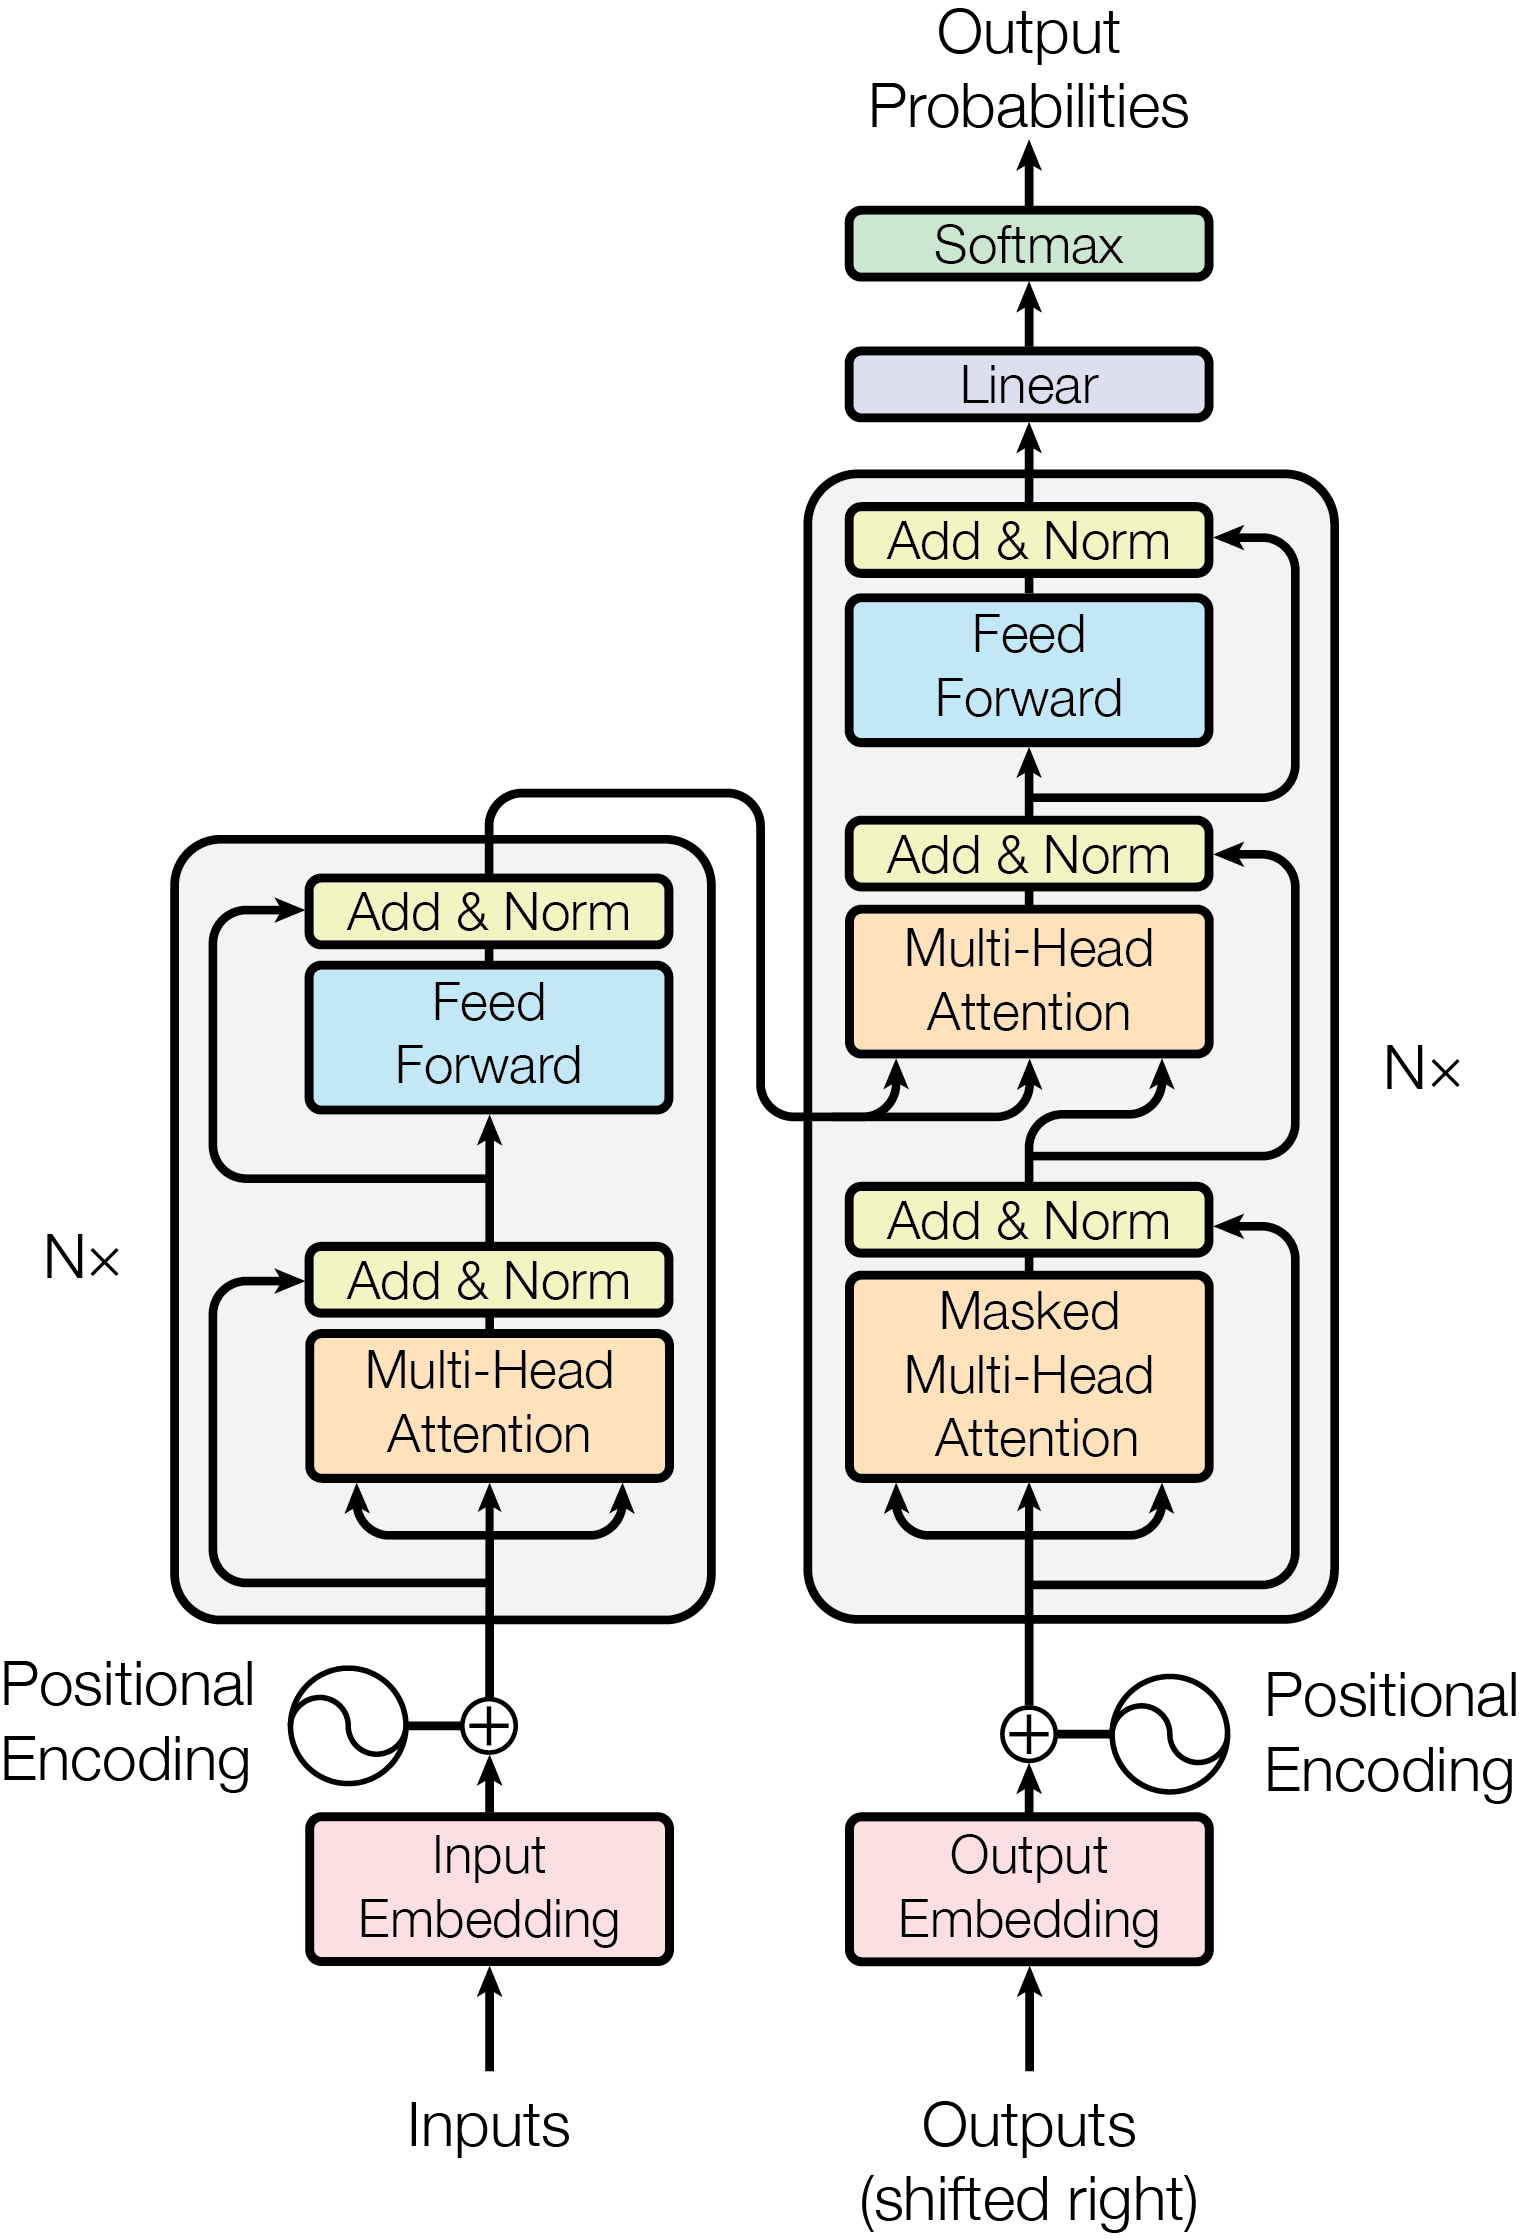
\includegraphics[width=0.5\linewidth]{chapter_3_theoretical_background/transformer.png}
	\caption{Overview of the Transformer architecture}
	Source: \textit{Attention Is All You Need} \cite{vaswani2017attention}
	\label{fig:chapter_3_theoretical_background/transformer}
\end{figure}

The Transformer architecture consists of an encoder and a decoder. The encoder takes as input a sequence of embeddings, such as word embeddings or character embeddings, and produces a sequence of hidden states that capture the information in the input sequence. The decoder takes as input the encoder hidden states and produces a sequence of output embeddings that represent the output sequence.

The encoder consists of multiple layers, each of which contains two sub-layers: a self-attention sub-layer and a feedforward sub-layer. In the self-attention sub-layer, the model computes a representation of each element in the input sequence by attending to all the other elements in the sequence. The feedforward sub-layer applies a pointwise fully connected layer to each position in the sequence independently and identically.

The decoder also consists of multiple layers, each of which contains three sub-layers: a self-attention sub-layer, a cross-attention sub-layer, and a feedforward sub-layer. In the self-attention sub-layer, the model attends to the previously generated output embeddings to compute the next output embedding. In the cross-attention sub-layer, the model attends to the encoder hidden states to incorporate information from the input sequence. The feedforward sub-layer applies a pointwise fully connected layer to each position in the sequence independently and identically.

The Transformer architecture uses residual connections and layer normalization to facilitate training of deep neural networks. Residual connections allow information to flow directly from one layer to another, bypassing the intermediate layers, which can help prevent the vanishing gradient problem. Layer normalization normalizes the input to each sub-layer to have zero mean and unit variance, which can help stabilize the training process.

Overall, the Transformer architecture has achieved state-of-the-art results on a wide range of natural language processing tasks, and its success has led to the development of a variety of transformer-based architectures, such as BERT, GPT, and T5.

\subsection{Graphs}
\label{subsec:3_graphs}

% https://arxiv.org/abs/2204.07697
% http://www.deepnlp.org/blog/latex-code-graph-neural-network
% https://towardsdatascience.com/graph-convolutional-networks-deep-99d7fee5706f
% https://www.datacamp.com/tutorial/comprehensive-introduction-graph-neural-networks-gnns-tutorial

A Graph is the type of data structure that contains nodes and edges. A node can be a person, place, or thing, and the edges define the relationship between nodes. The edges can be directed and undirected based on directional dependencies. 

Graphs are excellent in dealing with complex problems with relationships and interactions. They are used in pattern recognition, social networks analysis, recommendation systems, and semantic analysis. Creating graph-based solutions is a whole new field that offers rich insights into complex and interlinked datasets. 

Nevertheless, Graph-based data structures have drawbacks, and researchers must understand them before developing graph-based solutions.

\begin{itemize}
	\item A graph exists in non-euclidean space. It does not exist in 2D or 3D space, which makes it harder to interpret the data. To visualize the structure in 2D space, you must use various dimensionality reduction tools.
	\item Graphs are dynamic; they do not have a fixed form. There can be two visually different graphs, but they might have similar adjacency matrix representations. It makes it difficult for us to analyze data using traditional statistical tools.
	\item Large size and dimensionality will increase the graph's complexity for human interpretations. The dense structure with multiple nodes and thousands of edges is harder to understand and extract insights. 
\end{itemize}

\subsubsection{Graph Neural Networks}
\label{subsubsec:3_gnns}

GNNs are a class of neural networks that operate on graphs, which are collections of nodes and edges. A typical graph is represented by a set of node features, represented by a matrix $X \in \mathbb{R}^{N \times D}$, where $N$ is the number of nodes, and $D$ is the number of features associated with each node. Each node is also connected to other nodes via edges, which are represented by an adjacency matrix $A \in {0,1}^{N \times N}$, where $A_{ij} = 1$ if there is an edge between nodes $i$ and $j$, and $0$ otherwise.

\begin{itemize}
	\item A graph exists in non-euclidean space. It does not exist in 2D or 3D space, which makes it harder to interpret the data. To visualize the structure in 2D space, you must use various dimensionality reduction tools.
	\item Graphs are dynamic; they do not have a fixed form. There can be two visually different graphs, but they might have similar adjacency matrix representations. It makes it difficult for us to analyze data using traditional statistical tools.
	\item Large size and dimensionality will increase the graph's complexity for human interpretations. The dense structure with multiple nodes and thousands of edges is harder to understand and extract insights. 
\end{itemize}

The basic idea behind GNNs is to iteratively update the node representations using information from the graph neighborhood. Specifically, at each iteration, each node aggregates information from its neighbors, and the resulting aggregated representation is used to update the node's own representation. This process is typically repeated for multiple iterations until convergence. GNNs were introduced when Convolutional Neural Networks failed to achieve optimal results due to the arbitrary size of the graph and complex structure. 

One common way to implement this idea is to use the following update rule:

\begin{equation}
h_i^{(l+1)} = f(h_i^{(l)}, \sum_{j} A_{ij} h_j^{(l)})
\end{equation}

where $h_i^{(l)}$ is the representation of node $i$ at iteration $l$, $f$ is a non-linear activation function, and $\sum_{j} A_{ij} h_j^{(l)}$ is the sum of the representations of the neighbors of node $i$ at iteration $l$.

By stacking multiple layers of such updates, a GNN can learn increasingly complex representations of the graph.

There are several types of neural networks, such as:

\begin{itemize}
	\item Graph Auto-Encoder Networks, which learn graph representation using an encoder and attempt to reconstruct input graphs using a decoder. They are commonly used in link prediction as Auto-Encoders are good at dealing with class balance. 
	\item Recurrent Graph Neural Networks(RGNNs) are able to learn the best diffusion pattern, and they can handle multi-relational graphs where a single node has multiple relations. They are commonly used in generating text, machine translation, speech recognition or generating image descriptions
	\item Gated Graph Neural Networks (GGNNs) improve Recurrent Graph Neural Networks by adding a node, edge, and time gates on long-term dependencies, being the common uses similar to RGNNs.
\end{itemize}

Nevertheless, in this work we focus on a particular type of GNN, that is, Graph Convolutional Networks, which are the most common GNN type used in of \ac{MP} in the field of \ac{AD}.

\subsubsection{Graph Convolutional Networks}
\label{subsubsec:3_gcns}

The majority of GNNs are Graph Convolutional Networks (GCNs), which are a specific type of GNN that use convolutional operations to aggregate information from the graph neighborhood. GCNs were introduced when Convolutional Neural Networks failed to achieve optimal results due to the arbitrary size of the graph and complex structure. The basic idea behind GCNs is to treat the graph as a signal and use convolutional operations to extract features by inspecting neighboring nodes. GCNs aggregate node vectors, pass the result to the dense layer, and apply non-linearity using the activation function. 

\begin{figure}[h]
	\centering
	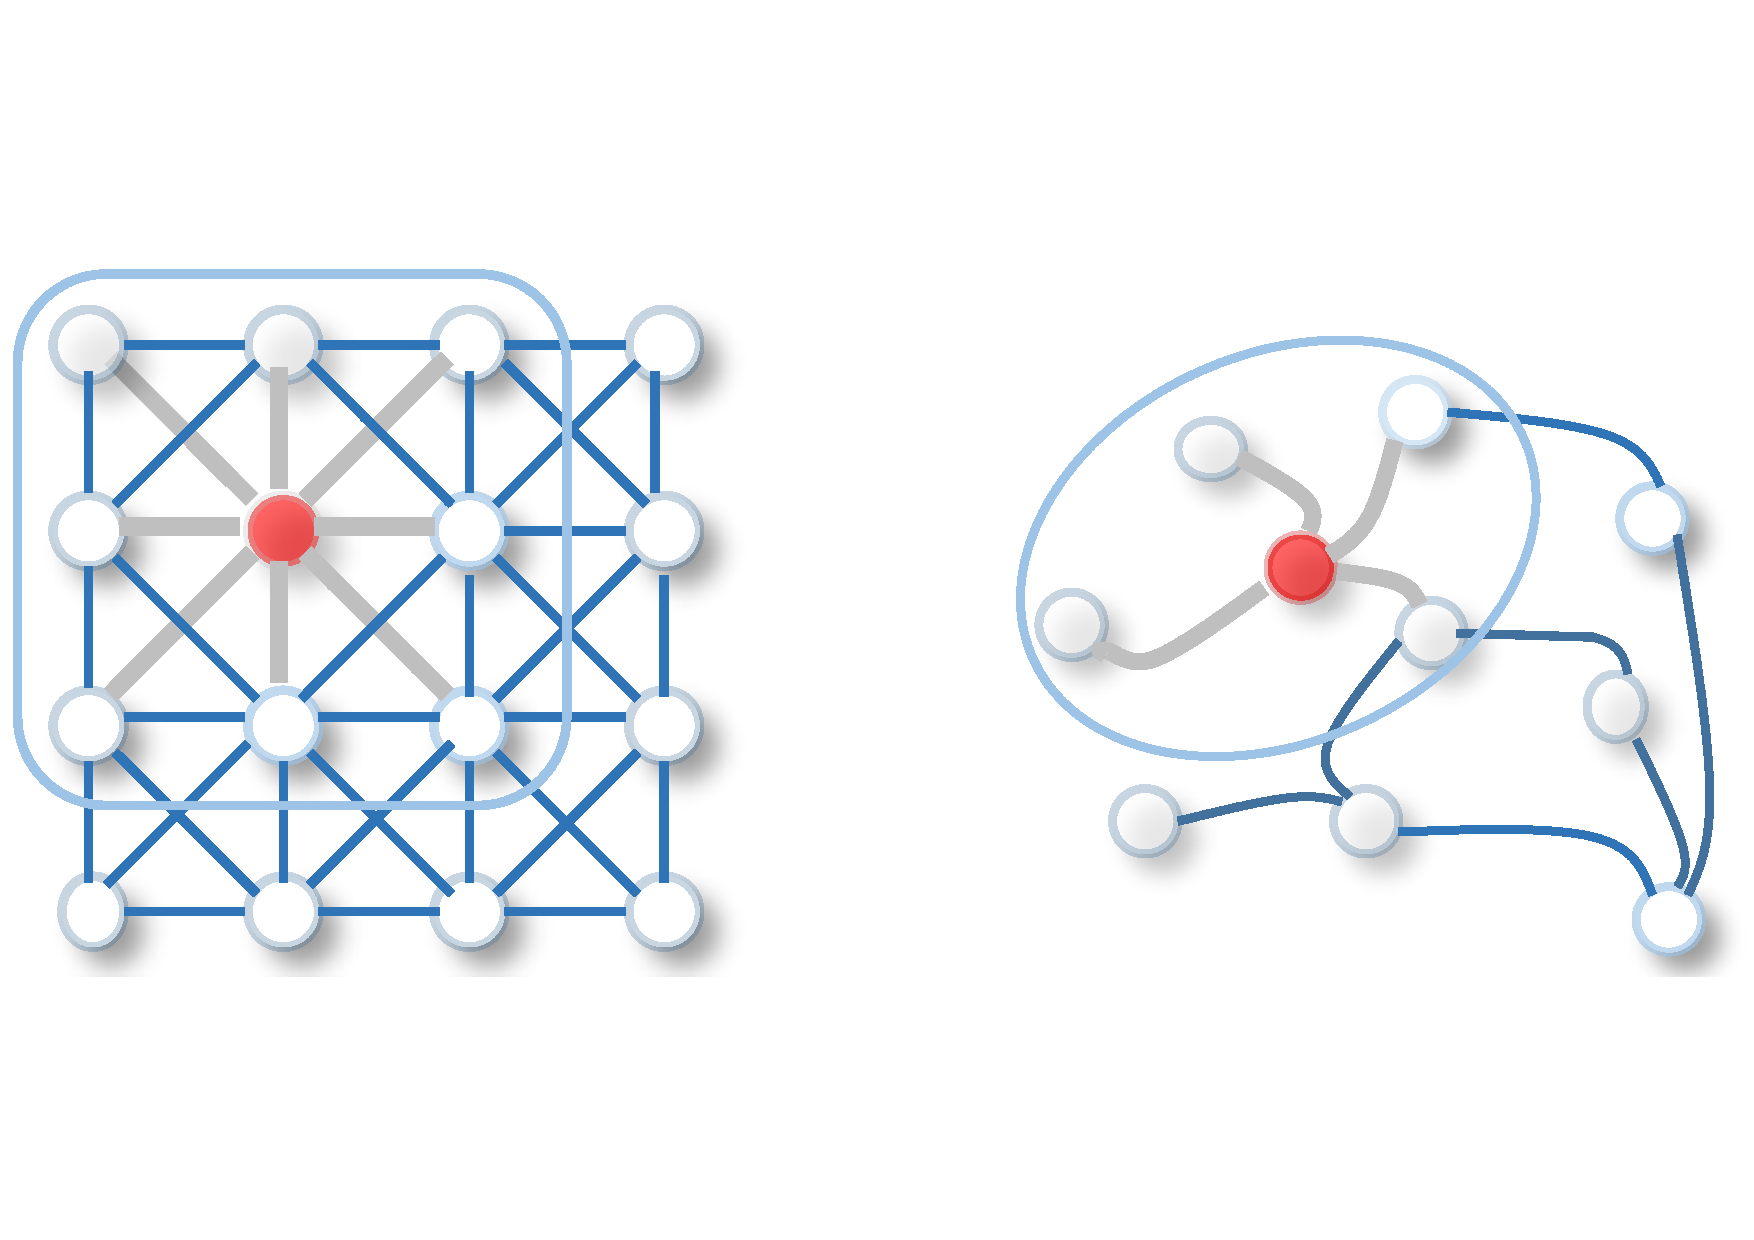
\includegraphics[width=0.6\linewidth]{chapter_3_theoretical_background/gcn_vs_cnn.pdf}
	\caption{Overview of the sliding kernel of a 2D-CNN vs GCN}
	Source: \textit{A comprehensive survey on graph neural networks} \cite{wu2020comprehensive}
	\label{fig:chapter_3_theoretical_background/gcn_vs_cnn}
\end{figure}

The major difference between GCN and CNN is that it is developed to work on non-euclidean data structures where the order of nodes and edges can vary, as it can be appreciated in Figure \ref{fig:chapter_3_theoretical_background/gcn_vs_cnn}. In 2D convolution, each pixel in an image is taken as a node where neighbours are determined by the filter size. The 2D convolution takes the weighted average of pixel values of the red node along with its neighbors. The neighbours of a node are ordered and have a fixed size. On the other hand, to get a hidden representation of a given node red, one simple solution of the graph convolutional operation is to take the average value of the node features of the red node along with its neighbors. Different from image data, the neighbors of a node are unordered and variable in size.

The convolution in GCN is the same as a convolution in convolutional neural networks. It multiplies neurons with weights (filters) to learn from data features. A convolutional operation on a graph is defined as:

\begin{equation}
H^{(l+1)} = \sigma(D^{-\frac{1}{2}} A D^{-\frac{1}{2}} H^{(l)} W^{(l)})
\end{equation}

where $H^{(l)}$ is the matrix of node representations at iteration $l$, $W^{(l)}$ is the weight matrix of the $l$-th layer, $A$ is the adjacency matrix of the graph, $D$ is the degree matrix of the graph, and $\sigma$ is a non-linear activation function.

The operation $D^{-\frac{1}{2}} A D^{-\frac{1}{2}}$ is a normalization step that scales the adjacency matrix by the inverse square root of the degree matrix. This normalization ensures that nodes with different degrees have similar influence in the convolutional operation. By stacking multiple layers of such convolutions, a GCN can learn increasingly complex features of the graph.

\subsection{Training}
\label{subsec:3_training}

Training is the process of iterating through a dataset to make the network learn the optimal mapping (combination of weights) from input to desired output in the data samples. In each iteration, a forward pass through the network is performed, computing the output of each layer until the end. This produces the output response of the network, which is then compared to a desired output with a defined Loss function (L). This function estimates the amount of error, which is back-propagated through the network to update its weights with the aim of minimizing the error. 

Regarding the supervised training paradigm, Backpropagation is an algorithm used for training artificial neural networks (ANNs) used to update the weights and biases of the neurons in the network based on the error between the predicted output and the actual output.

The backpropagation algorithm consists of two phases: the forward pass and the backward pass. During the forward pass, the input is fed into the network and propagated through the layers to obtain the predicted output. During the backward pass, the error between the predicted output and the actual output is computed and used to update the weights and biases of the neurons in the network.

The backpropagation algorithm is based on the chain rule of calculus, which allows the gradient of the loss function with respect to each weight and bias to be computed recursively from the output layer to the input layer of the network. The gradient descent algorithm is then used to update the weights and biases in the direction of the negative gradient of the loss function. In that sense, the main losses used in this work are described throughout the remaining content of this Chapter.

\subsubsection{Optimizer and learning rate}
\label{subsubsec:3_optimizer_and_lr}

There are several optimizers commonly used for training deep neural networks in the literature, such as Stochastic Gradient Descent (SGD) \cite{robbins1951stochastic}, Adagrad \cite{duchi2011adaptive}, Root Mean Square Propagation (RMSprop) \cite{zou2019sufficient} or Adadelta \cite{zeiler2012adadelta}. In this work we use one of the most extended, the ADAM \cite{kingma2014adam} optimizer. It is a popular optimization algorithm used in deep learning, particularly for training neural networks. It is an adaptive learning rate optimization algorithm that is well suited for large datasets and high-dimensional parameter spaces.

The basic idea behind ADAM is to compute adaptive learning rates for each parameter based on estimates of the first and second moments of the gradients. The algorithm computes a moving average of the gradients and their squared values, and uses these estimates to update the parameters with a learning rate that adapts to the local curvature of the loss function. The algorithm also includes bias-correction terms to ensure that the estimates are unbiased, especially in the early stages of training when the estimates are highly uncertain.

The update rule for ADAM can be expressed mathematically as follows:

\begin{equation}
\begin{split}
	m_t &= \beta_1 m_{t-1} + (1-\beta_1) g_t \\
	v_t &= \beta_2 v_{t-1} + (1-\beta_2) g_t^2 \\
	\hat{m}_t &= \frac{m_t}{1-\beta_1^t} \\
	\hat{v}t &= \frac{v_t}{1-\beta_2^t} \\
	\theta{t+1} &= \theta_t - \frac{\alpha}{\sqrt{\hat{v}_t}+\epsilon} \hat{m}_t
\end{split}
\end{equation}

where $\theta_t$ is the parameter vector at time step $t$, $g_t$ is the gradient vector, $m_t$ and $v_t$ are the first and second moment estimates at time step $t$, $\hat{m}_t$ and $\hat{v}_t$ are the bias-corrected moment estimates, $\alpha$ is the learning rate, $\beta_1$ and $\beta_2$ are the decay rates for the moment estimates, and $\epsilon$ is a small constant to prevent division by zero.

The algorithm starts with initializing $m_0$ and $v_0$ as zero vectors, and $\theta_0$ as the initial parameter vector. At each iteration, the gradient vector $g_t$ is computed using a batch of training data, and the moment estimates $m_t$ and $v_t$ are updated according to the first two lines of the update rule. The bias-corrected moment estimates $\hat{m}_t$ and $\hat{v}_t$ are then computed using the next two lines of the update rule. Finally, the parameter vector $\theta_t$ is updated using the last line of the update rule.

The hyperparameters $\alpha$, $\beta_1$, $\beta_2$, and $\epsilon$ can be tuned to optimize performance on a particular dataset and neural network architecture.

On the other hand, The learning rate is a key hyperparameter in the optimization process of machine learning algorithms, including optimizer updates like the ADAM optimizer. The learning rate controls the step size taken in the direction of the negative gradient during each iteration of the optimization process.

If the learning rate is too small, the optimization process will be slow and may get stuck in local minima. On the other hand, if the learning rate is too large, the optimization process may overshoot the minimum and oscillate back and forth, or even diverge.

In the context of the ADAM optimizer, the learning rate is used to adjust the size of the update step taken in the direction of the estimated gradient. The update step is multiplied by the learning rate, which determines the size of the step. A larger learning rate will result in larger update steps, and a smaller learning rate will result in smaller update steps.

In practice, the learning rate is usually set through a process called hyperparameter tuning, where different values of the learning rate are tried on a validation set to find the optimal value that results in the best performance of the model on the test set.

One common technique to adjust the learning rate during training is called learning rate scheduling. This involves decreasing the learning rate over time, often according to a predetermined schedule or based on the performance of the model on a validation set. This technique can help improve the convergence and stability of the optimization process, particularly in the later stages of training when the model is close to the optimal solution.

Overall, the learning rate plays a crucial role in the optimization process of machine learning algorithms, including optimizer updates like the ADAM optimizer. Selecting an appropriate learning rate is important for achieving fast and stable convergence to the optimal solution.

\subsubsection{Regression losses}
\label{subsec:3_regression_losses}

% https://blmoistawinde.github.io/ml_equations_latex/

A regression loss is a type of loss function used in regression problems to measure the difference between the predicted and true values of a continuous variable. In other words, it is a way to quantify how well a machine learning model is able to predict numerical values based on input data.

In regression problems, the goal is to learn a function that maps input features to output values. A regression loss is used to train the model by penalizing the difference between the predicted and true output values. The loss function is typically minimized during training, so that the model learns to make more accurate predictions. There are several types of regression loss functions, such as the Quantile loss, Log-Cosh or Mean Absolute Error (MAE). In this work we mainly focus on the Mean Square Error (MSE) and SmoothL1, also known as Huber loss.

\paragraph{Mean Square Error loss}
\label{par:3_mse_loss}

The Mean Squared Error (MSE) loss is a commonly used loss function in regression problems. It measures the average squared difference between the predicted and true values of a continuous variable. The MSE loss is given by:

\begin{equation}
	MSE(y, \hat{y}) = \frac{1}{n}\sum_{i=1}^{n}(y_i - \hat{y_i})^2
\end{equation}

where $y_i$ is the true value of the $i$-th data point, $\hat{y_i}$ is the predicted value, and $n$ is the number of data points.

The MSE loss penalizes large errors more strongly than small errors, since it uses the square of the difference between the predicted and true values. This makes it sensitive to outliers and can lead to overfitting if the data contains extreme values.

The MSE loss is used in many regression problems, such as linear regression, polynomial regression, and neural networks. It is often used as a performance metric to evaluate the quality of the model's predictions.

\paragraph{SmoothL1 loss}
\label{par:3_smoothL1_loss}

SmoothL1 loss, also known as Huber loss, is a loss function used in regression problems to measure the difference between the predicted and true values of a continuous variable. It is a variant of the L1 loss that is less sensitive to outliers and has a smooth gradient near zero.

The SmoothL1 loss function can be defined as follows:

\begin{equation}
\begin{split}
	L(y, \hat{y}) = \begin{cases}
		\frac{1}{2}(y - \hat{y})^2 & \text{if } |y - \hat{y}| < 1 \\
		|y - \hat{y}| - \frac{1}{2} & \text{otherwise} \
	\end{cases}
\end{split}
\end{equation}

where $y$ is the true value, $\hat{y}$ is the predicted value, and $|\cdot|$ represents the absolute value function.

The SmoothL1 loss function behaves like the L1 loss for small errors and like the L2 loss for large errors. Specifically, for errors smaller than 1, it uses the squared difference between the predicted and true values, which has a smooth gradient. For larger errors, it uses the absolute difference, which is less sensitive to outliers than the squared difference.

The SmoothL1 loss is used in regression problems when the data contains outliers or when the model needs to be less sensitive to large errors. It is commonly used in object detection and localization tasks, where the predicted bounding boxes can be highly sensitive to small changes in the input data.

\paragraph{Softmax loss}
\label{par:3_softmax_loss}

The softmax loss, also known as the cross-entropy loss, is a commonly used loss function in classification problems. It measures the difference between the predicted probability distribution and the true probability distribution of a categorical variable. The softmax loss is given by:

\begin{equation}
	CE(y, \hat{y}) = -\frac{1}{n}\sum_{i=1}^{n}\sum_{j=1}^{k} y_{i,j}\log(\hat{y_{i,j}})
\end{equation}

where $y_{i,j}$ is the true probability of the $i$-th data point belonging to class $j$, $\hat{y_{i,j}}$ is the predicted probability, $n$ is the number of data points, and $k$ is the number of classes.

The softmax function is applied to the output of the model to obtain a probability distribution over the classes. The predicted probability of class $j$ is given by:

\begin{equation}
	\hat{y_{i,j}} = \frac{e^{z_{i,j}}}{\sum_{l=1}^{k} e^{z_{i,l}}}
\end{equation}

where $z_{i,j}$ is the unnormalized score or logit for class $j$ of the $i$-th data point.

The softmax loss penalizes the model more heavily for predictions that are far from the true probabilities. It encourages the model to assign higher probabilities to the correct classes and lower probabilities to the incorrect classes.

The softmax loss is used in many classification problems, such as image classification, natural language processing, and speech recognition. It is often used as a performance metric to evaluate the quality of the model predictions.

\paragraph{Negative Log-Likelihood loss}
\label{par:3_NLL_loss}

Negative Log Likelihood (NLL) loss is a loss function commonly used in classification problems, particularly in deep learning models that output probabilities for each class. It is a type of maximum likelihood estimation (MLE) loss, which means it attempts to maximize the likelihood of the predicted probabilities given the true labels.

The NLL loss function can be defined as follows:

\begin{equation}
	L(y_i, \hat{y_i}) = -\log(\hat{y_{i,y_i}})
\end{equation}

where $y_i$ is the true label of the $i$-th data point, $\hat{y_i}$ is the predicted probability distribution for that point, and $\hat{y_{i,y_i}}$ is the predicted probability for the true label.

The NLL loss penalizes the model for assigning low probabilities to the true label, while rewarding it for assigning high probabilities. It is a logarithmic loss function, which means that the penalty for low probabilities increases exponentially as the predicted probability approaches zero.

The NLL loss is used in classification problems because it provides a gradient that can be used to update the model parameters during training, in order to improve the accuracy of the predicted probabilities. It is commonly used in conjunction with softmax activation function, which ensures that the predicted probabilities sum to one across all classes.

\paragraph{Winner-Takes-All loss}
\label{par:3_WTA_loss}

Winner-Takes-All (WTA) loss is a loss function used in clustering problems, particularly in competitive learning models. It is a type of unsupervised learning, which means that it does not require labeled data for training.

The WTA loss function can be defined as follows:

\begin{equation}
\begin{split}
	L(y_i, f(x_i)) = \begin{cases}
		0 & \text{if } y_i = \arg\max_j f_j(x_i) \\
		1 & \text{otherwise} \
	\end{cases}
\end{split}
\end{equation}

where $y_i$ is the true cluster of the $i$-th data point, $f_j(x_i)$ is the activation of the $j$-th neuron in the output layer for that point, and $\arg\max_j f_j(x_i)$ is the index of the neuron with the highest activation.

The WTA loss function penalizes the model for assigning a data point to the wrong cluster. It works by forcing each neuron in the output layer to specialize in a particular cluster, such that the neuron with the highest activation for a given point corresponds to the true cluster of that point.

The WTA loss is used in clustering problems because it encourages the model to learn a set of representative clusters that capture the structure of the data, without requiring any prior knowledge of the true labels. It is commonly used in conjunction with competitive learning algorithms, such as self-organizing maps (SOMs), that use local competition between neurons to learn a topology-preserving mapping from the input space to the output space.

\paragraph{Hinge loss}
\label{par:3_hinge_loss}

Hinge loss is a loss function used in classification problems, particularly in support vector machines (SVMs). It is a type of max-margin loss, which means it attempts to maximize the margin between the decision boundary and the data points.

The hinge loss function can be defined as follows:

\begin{equation}
	L(y_i, f(x_i)) = \max(0, 1 - y_i f(x_i))
\end{equation}

where $y_i$ is the true label of the $i$-th data point, $f(x_i)$ is the predicted score for that point, and $1$ is a margin hyperparameter that determines the width of the margin.

If $y_i f(x_i) \geq 1$, then the point is correctly classified and the loss is zero. If $y_i f(x_i) < 1$, then the point is misclassified and the loss is proportional to the distance between the predicted score and the correct score. The loss function penalizes misclassifications linearly, with a slope of -1 for negative misclassifications and 0 for positive misclassifications.

The hinge loss is used in SVMs because it encourages the model to find a decision boundary that maximizes the margin between the classes, while still correctly classifying the data points. This results in a more robust and generalizable model.

\subsubsection{Regularization techniques}
\label{subsubsec:3_regularization}

Regularization techniques in deep learning are used to prevent overfitting and improve the generalization performance of a model. Overfitting occurs when a model fits the training data too closely and captures noise or irrelevant patterns, resulting in poor performance on new, unseen data. Here are some commonly used regularization techniques in deep learning:

L1 and L2 regularization: L1 and L2 regularization are two popular regularization techniques that add a penalty term to the loss function during training. L1 regularization adds the sum of the absolute values of the weights to the loss function, while L2 regularization adds the sum of the squares of the weights. This encourages the model to learn simpler and more generalizable representations by shrinking the weights towards zero.

Dropout: Dropout is a regularization technique that randomly drops out some units (neurons) in a layer during training. This forces the remaining units to learn more robust and diverse representations that generalize better to new data. Dropout has been shown to be effective in reducing overfitting, particularly in deep neural networks with many layers.

Data augmentation: Data augmentation is a technique that artificially increases the size of the training set by generating new examples from existing ones. This can be done by applying transformations such as rotations, translations, flips, or adding noise to the input data. Data augmentation can help reduce overfitting by increasing the diversity of the training data and improving the generalization performance of the model.

Early stopping: Early stopping is a technique that monitors the performance of the model on a validation set during training and stops the training process when the performance starts to degrade. This prevents the model from overfitting to the training data and allows it to generalize better to new data.

Batch normalization: Batch normalization is a technique that normalizes the activations of a layer by subtracting the batch mean and dividing by the batch standard deviation. This helps stabilize the distribution of the activations and reduces the internal covariate shift, which can improve the training process and reduce overfitting.

Weight decay: Weight decay is a technique that adds a penalty term to the loss function during training, similar to L2 regularization. The penalty term is proportional to the square of the weights, and it encourages the model to learn smaller and simpler weights, which can reduce overfitting.

These are some of the commonly used regularization techniques in deep learning. They can be combined and tuned to improve the performance of a model on a specific task and dataset.

Moreover, another interesting technique to help the model improve during training is hard-mining. Hard-mining is a technique in deep learning used to improve the training of a model by focusing on the samples that are most difficult to classify correctly.

During training, the model makes predictions on a batch of training data, and the loss function is computed based on the difference between the predicted values and the true values. In hard-mining, the training samples that contribute the most to the loss function are identified, and these samples are given more importance during training.

The idea behind hard-mining is that by focusing on the difficult samples, the model is forced to learn more discriminative features that can better distinguish between the different classes. This can lead to better generalization performance and improved accuracy on the test data.

There are several ways to implement hard-mining in deep learning, including:

\begin{itemize}
	\item Hard negative mining involves selecting the training samples that are misclassified with the highest confidence by the model and including them in the next batch of training data. By focusing on the difficult negative samples, the model can learn to better distinguish between the different classes and reduce the number of false negatives.
	
	\item Hard positive mining involves selecting the training samples that are misclassified with the lowest confidence by the model and including them in the next batch of training data. By focusing on the difficult positive samples, the model can learn to better distinguish between the different classes and reduce the number of false positives.
	
	\item Curriculum learning involves gradually increasing the difficulty of the training data over time. The model is first trained on easy samples and then gradually exposed to more difficult samples. This can help the model learn more robust and generalizable features by gradually increasing the complexity of the training data.
	
	\item Overall, hard-mining is a useful technique in deep learning for improving the training of a model by focusing on the difficult samples. By incorporating hard-mining into the training process, the model can learn more discriminative features and improve its generalization performance on new, unseen data.
\end{itemize}

\section{Summary}
\label{sec:3_summary}

In this chapter, the mathematical background of various physics-based and \ac{DL}-based techniques used for \ac{MP} models is thoroughly examined. The chapter aims to provide a comprehensive understanding of these methods and their applications in the field of motion prediction.

The chapter begins by introducing the physics-based techniques, starting with the Kalman Filter. The Kalman Filter is a recursive algorithm used to estimate the state of a dynamic system by incorporating noisy measurements. Its mathematical foundation, including the state-space model and the prediction and update steps, is discussed in detail. Next, the Hungarian Algorithm is presented, which is a combinatorial optimization algorithm used for data association in multiple object tracking. The chapter delves into the mathematical formulation of the Hungarian Algorithm and how it can be applied to motion prediction tasks.

Moving on to the physics-based models, the chapter explores the \ac{CTRV} and \ac{CTRA} models. These models are widely used for trajectory prediction and capture the motion dynamics of objects by considering their position, velocity, and acceleration. The mathematical equations for these models are examined, highlighting how they can be utilized to predict future motion paths.

The chapter then transitions to deep learning-based techniques, which have gained significant attention in recent years due to their ability to capture complex patterns and dependencies in data. Several models are discussed in detail, starting with the 1D-Convolutional Neural Network (CNN). The mathematical architecture of the 1D-CNN is explained, emphasizing its ability to extract spatial and temporal features from sequential data for motion prediction.

Next, the \ac{LSTM} model is introduced, which is a type of recurrent neural network (RNN) specifically designed to handle sequence data. The chapter provides an overview of the \ac{LSTM} architecture, including its memory cell and gate mechanisms, which enable it to capture long-term dependencies and predict future motion accurately.

The chapter then explores \acp{GAN} and their application in motion prediction. \acp{GAN} consist of a generator and discriminator network that compete against each other, resulting in the generation of realistic and coherent motion trajectories. The mathematical formulation of \acp{GAN} and their training process are examined in detail.

Furthermore, the Graph Convolutional Network (GCN) is discussed, which is a deep learning model capable of operating on graph-structured data. The chapter explains how GCNs can be used to represent and predict motion patterns in scenarios where objects interact with each other.

Finally, the Attention mechanism is examined, which is a component commonly integrated into deep learning models to focus on relevant parts of the input data. The chapter explores the mathematical formulation of the Attention mechanism and its application in motion prediction models, highlighting its ability to assign different weights to different input features based on their relevance.

Overall, this chapter provides a comprehensive overview of the mathematical foundations of various physics-based and deep learning-based techniques used in motion prediction models. By understanding the underlying principles and equations of these models, researchers and practitioners can gain a deep understanding of their capabilities and make informed decisions regarding their application in different scenarios.
%%%%%%%%%%%%%%%%%%%%%%%%%%%%%%%%%%%%%%%%%%%%%%%%%%%%%%%%%%%%%%%%%%%%%%%%%%% 
% 
% Generic template for TFC/TFM/TFG/Tesis
% 
% By:
% + Javier Macías-Guarasa. 
% Departamento de Electrónica
% Universidad de Alcalá
% + Roberto Barra-Chicote. 
% Departamento de Ingeniería Electrónica
% Universidad Politécnica de Madrid   
% 
% Based on original sources by Roberto Barra, Manuel Ocaña, Jesús Nuevo,
% Pedro Revenga, Fernando Herránz and Noelia Hernández. Thanks a lot to
% all of them, and to the many anonymous contributors found (thanks to
% google) that provided help in setting all this up.
% 
% See also the additionalContributors.txt file to check the name of
% additional contributors to this work.
% 
% If you think you can add pieces of relevant/useful examples,
% improvements, please contact us at (macias@depeca.uah.es)
% 
% You can freely use this template and please contribute with
% comments or suggestions!!!
% 
%%%%%%%%%%%%%%%%%%%%%%%%%%%%%%%%%%%%%%%%%%%%%%%%%%%%%%%%%%%%%%%%%%%%%%%%%%% 

\chapter{Predictive Techniques for Scene Understanding}
\label{cha:predictive_techniques}

\begin{FraseCelebre}
	\begin{Frase}
		Avanzad, sin temor a la oscuridad. \\
		Luchad jinetes de Theoden. \\
		Caerán las lanzas, se quebrarán los escudos. \\
		Aún restará la espada. \\
		Rojo será el día, hasta el nacer del sol. \\
		Cabalgad, cabalgad, cabalgad hacia la desolación \\ 
		y el fin del mundo. Muerte, muerte, muerte.
	\end{Frase}
	\begin{Fuente}
		Discurso de Theoden, Rey de Rohan \\
		El Señor de los Anillos: El Retorno del Rey
	\end{Fuente}
\end{FraseCelebre}

\section{SmartMOT}
\label{sec:4_smartmot}

\section{GAN based Vehicle Motion Prediction}
\label{sec:4_gan_lstm}

\section{Exploring Map Features}
\label{sec:4_mapfe4mp}

\section{Leveraging traffic context via GNN}
\label{sec:4_mapfe4mp_gnn}

\section{Improving efficiency of Vehicle Motion Prediction}
\label{sec:4_cghformer}
%%%%%%%%%%%%%%%%%%%%%%%%%%%%%%%%%%%%%%%%%%%%%%%%%%%%%%%%%%%%%%%%%%%%%%%%%%% 
% 
% Generic template for TFC/TFM/TFG/Tesis
% 
% By:
% + Javier Macías-Guarasa. 
% Departamento de Electrónica
% Universidad de Alcalá
% + Roberto Barra-Chicote. 
% Departamento de Ingeniería Electrónica
% Universidad Politécnica de Madrid   
% 
% Based on original sources by Roberto Barra, Manuel Ocaña, Jesús Nuevo,
% Pedro Revenga, Fernando Herránz and Noelia Hernández. Thanks a lot to
% all of them, and to the many anonymous contributors found (thanks to
% google) that provided help in setting all this up.
% 
% See also the additionalContributors.txt file to check the name of
% additional contributors to this work.
% 
% If you think you can add pieces of relevant/useful examples,
% improvements, please contact us at (macias@depeca.uah.es)
% 
% You can freely use this template and please contribute with
% comments or suggestions!!!
% 
%%%%%%%%%%%%%%%%%%%%%%%%%%%%%%%%%%%%%%%%%%%%%%%%%%%%%%%%%%%%%%%%%%%%%%%%%%% 

\chapter{Applications in Autonomous Driving}
\label{cha:applications_in_autonomous_driving}

\begin{FraseCelebre}
	\begin{Frase}
		La fuerza de tus convicciones determina tu éxito, \\
		no el número de tus seguidores.
	\end{Frase}
	\begin{Fuente}
		Reamus Lupin \\
		Harry Potter y Las Reliquias de la Muerte, Parte 2
	\end{Fuente}
\end{FraseCelebre}


\section{Motion Prediction Datasets}
\label{sec:5_datasets}

\section{Multi-Object Tracking}
\label{sec:5_mot}

\section{Decision-Making}
\label{sec:5_decision_making}

\section{Holistic Simulation}
\label{sec:5_simulation}
%%%%%%%%%%%%%%%%%%%%%%%%%%%%%%%%%%%%%%%%%%%%%%%%%%%%%%%%%%%%%%%%%%%%%%%%%%% 
% 
% Generic template for TFC/TFM/TFG/Tesis
% 
% By:
% + Javier Macías-Guarasa. 
% Departamento de Electrónica
% Universidad de Alcalá
% + Roberto Barra-Chicote. 
% Departamento de Ingeniería Electrónica
% Universidad Politécnica de Madrid   
% 
% Based on original sources by Roberto Barra, Manuel Ocaña, Jesús Nuevo,
% Pedro Revenga, Fernando Herránz and Noelia Hernández. Thanks a lot to
% all of them, and to the many anonymous contributors found (thanks to
% google) that provided help in setting all this up.
% 
% See also the additionalContributors.txt file to check the name of
% additional contributors to this work.
% 
% If you think you can add pieces of relevant/useful examples,
% improvements, please contact us at (macias@depeca.uah.es)
% 
% You can freely use this template and please contribute with
% comments or suggestions!!!
% 
%%%%%%%%%%%%%%%%%%%%%%%%%%%%%%%%%%%%%%%%%%%%%%%%%%%%%%%%%%%%%%%%%%%%%%%%%%% 

\chapter{Conclusions and Future Works}
\label{cha:conclusions_and_future_works}

\begin{FraseCelebre}
	\begin{Frase}
		El mundo no es todo alegría y color, es un lugar terrible y por muy duro que seas es capaz de arrodillarte a golpes y tenerte sometido a golpes permanente si no se lo impides; Ni tú ni yo ni nadie golpea mas fuerte que la vida. Pero no importa lo fuerte que golpeas, sino lo fuerte que pueden golpearte y los aguantas mientras avanzas, hay que soportar sin dejar de avanzar.
		
		¡Así es como se gana!
		
		Si tú sabes lo que vales, vé y consigue lo que mereces pero tendrás que soportar los golpes y no puedes estar diciendo que no estás donde querías llegar por culpa de él o de ella, eso lo hacen los cobardes y tú no lo eres.
		
		TÚ ERES CAPAZ DE TODO.
	\end{Frase}
	\begin{Fuente}
		Discurso de Rocky a su hijo \\
		Rocky Balboa
	\end{Fuente}
\end{FraseCelebre}

\section{Conclusions}
\label{sec:6_introduction}

In this thesis, a series of interaction-aware trajectory prediction methods, including single-agent trajectory prediction, multi-agent trajectory prediction, and multimodal trajectory prediction, are developed for autonomous driving. Besides, the
impacts of trajectory prediction on trajectory planning are also investigated.
In Chapter 3, a novel framework with consideration of vehicle-infrastructure heterogeneous interactions is proposed for trajectory prediction of a single target vehicle. In the proposed scheme, a heterogeneous graph is developed to represent
the interactions, where the nodes contain features extracted from corresponding
encoders. Besides, a novel heterogeneous graph social pooling (HGS) module is
designed to extract high-level interaction features. The framework can be easily expanded for highway driving scenarios. Experimental results obtained using
real-world driving datasets show that the proposed HGS method outperforms existing interaction-aware methods in terms of prediction accuracy. Besides, ablative
studies demonstrate that the consideration of vehicle-infrastructure heterogeneous
interactions effectively improves the prediction accuracy compared to those methods only considering inter-vehicle interactions.
Then, the above prediction method for single-agent is generalized and expanded
for heterogeneous multi-agent trajectory prediction in Chapter 4. To do this, a
novel three-channel framework is designed to jointly consider traffc participants’
dynamics, interaction, and map features. The driving scene is represented in a hybrid way, where the inter-agent interaction in the traffc system is represented with
an edge-featured heterogeneous graph, and the shared local map is represented
with a Bird’s Eye View (BEV) image. Two shared Recurrent Neural Networks
(RNNs) are adopted to capture vehicles’ and pedestrians’ dynamics features from
their historical states, respectively. A novel heterogeneous edge-enhanced graph
attention network (HEAT) is proposed to model the inter-agent interactions, and
a map-sharing technique based on the gate mechanism is also leveraged to share the
local map across all target agents. Experimental validations on real-world driving
datasets of both urban and highway scenarios show that the proposed method not
only achieves state-of-the-art performance but also can provide simultaneous predictions of multi-agent trajectories for a variable number of heterogeneous agents.
Besides the unimodal predictions for single and multiple agents, this thesis also
tackles the inherent multimodality problem of driving behaviors for prediction in
Chapter 5. A novel map-adaptive multimodal trajectory prediction framework is
proposed. Within this framework, through a single graph operation, a variable
number of map-compliant trajectories and a non-map-compliant trajectory can be
generated. Map-compliant predictions are conditioned on either a single candidate
centerline (CCL) or a bunch of all CCLs, making the predictor adaptive to different
road structures. The non-map-compliant prediction captures the irrational driving
behavior for safety concerns. The driving scene is represented with a heterogeneous
hierarchical graph containing both agents and their CCLs. A hierarchical graph
operator (HGO) with an edge-masking technology is proposed to encode the driving
scene. Validation on the Argoverse motion forecasting benchmark shows that the
proposed method achieves state-of-the-art performance with the advantage of mapadaptive capacity.
Beyond pure prediction, in Chapter 6, predictive planning and the impacts of prediction on downstream trajectory planning are also investigated. An interactionaware predictive planner, which is trained to imitate human driving behaviors,
is designed to investigate the problem of how prediction would affect the performance of motion planning. The predictive planner is obtained by training an
oracle planner, which is aware of target agents’ ground truth future trajectories,
and replacing the ground truth with the predicted trajectories for inference during
implementation. Experimental results on a real-world dataset show that the proposed predictive planner achieves better performance over other baselines in terms
of displacement error, miss rate, and collision rate. The gap between the predictive
planner and the oracle planner shows that it is promising to further enhance the
planning performance by improving the prediction accuracy.
To be implemented in real-world self-driving systems, the proposed methods require upstream localization, perception, and tracking results, since the historical
states of other traffc participants are needed as the input of the proposed methods. Perception can be realized using either or both of camera and LiDAR. Other
sensors, such as radar, can also be used for better perception via sensor fusion. For
the single-agent and multi-agent prediction methods in Chapter 3 and Chapter 4,
we are using BEV maps, where only the map is needed. We do not need a BEV
image to show the real-time tra!c. The map can be obtained from main-stream
map providers and converted into images for the usage of our method. The mapadaptive multimodal method in Chapter 5, however, requires a high-definition map
(HD map) of the local area since we need the candidate centerlines of vehicles of interest. The methods can run on both CPUs or GPUs, and using GPUs is suggested
for faster inference.

\section{Future Works}
\label{sec:6_future_works}

Although many studies have been done in trajectory prediction and path planning
in the past years, there are still many aspects that need to be further investigated
in the future.
Scene representation and encoding. Researchers have proposed many methods
to encode driving scenes with different representations. However, there is no unified
representation of various driving scenes so far. The lack of a universal representation limits the generalizability of prediction methods with large-scale deployment
in autonomous vehicles in the real world because a method can hardly be applied
to a situation that cannot be described. Among many representation approaches
proposed so far, graph-based representations are promising because a graph can
accommodate an arbitrary number of heterogeneous objects and represent their
interdependencies via directed edges. For example, when modeling a driving scene
in the context of traffc systems, a node can represent a vehicle, a pedestrian, a
lanelet, a junction, a traffc signal, etc. A new object can always be added to the
existing graph. There are three important steps that need to be done to further
improve the graph-based scene representation and encoding in the future. The first
aspect is to construct the graph with proper connections, that is, to determine the
edge set of the graph. This step needs to identify interdependencies between pairs
of nodes and connect nodes with directed edges for information flow in the graph.
Once the graph structure is settled, the second step is to assign the node, and edge
features properly. This requires researchers to select or design proper encoders
for different kinds of nodes and edges. Then the third step is required to design
graph operators to handle the heterogeneity in the scene graphs. In this step, the
advances in heterogeneous graph neural networks can be leveraged.
Trajectory decoding. For future work, an immediate step is to generalize the
map-adaptive multimodal prediction method proposed in Chapter 5 with uncertainty estimations. The uncertainty includes both motion and mode uncertainties.
The motion uncertainty captures the distribution of agents’ position over a planar
map at each time step, and the mode uncertainty captures the possibility of driving
modalities. The former can be modeled via bivariate Gaussian distributions, and
the latter can be treated as a multi-class classification problem over a variable number of modalities. Then the next step can focus on generalizing uncertainty-aware
multimodal predictions to multi-agent settings by modeling the joint distribution
of multiple agents’ behaviors. Social consistency should be considered in this step
such that there is no conflict between any pair of trajectories in a joint modality
in normal cases. Besides, trajectory predictors should be designed from the ego
vehicle’s point of view. One possible way is to design a decoder that can output
trajectories upon the ego’s request. For example, the predictor can focus on a small
set of target agents requested by the ego vehicle rather than all the agents in sight.
For a specific target agent, the predictor can focus on predicting its driving options
that may affect the ego’s planned trajectories. This attentive approach can reduce
computation efforts for real-time implementations.
Predictive planning. The ultimate goal of trajectory prediction is to further
improve the performance of decision-making and motion control of autonomous
vehicles with respect to safety, smartness, and effciency. So prediction must be integrated into the planning module, and therefore predictive planning is worthwhile
exploring. There are many problems that should be addressed for the development
of predictive planners. First, predictive planners should be able to address prediction uncertainty since prediction can never be exactly the same as the ground truth.
Second, the relationship between prediction and planning needs to be further studied in order to answer the following questions: 1) How would the improvement in
prediction affect the downstream planning performance? 2) Is there a floor of prediction error below which improving prediction accuracy leads to no improvement
or even a negative effect on planning? 3) Can we design a predictive planner that
is scalable to predictors of different uncertainties as long as these uncertainties are
known? Third, learning-based motion planners should be further investigated since
they have great potential to be incorporated with data-driven predictions. However, the current limitations in explainability and reliability need to be addressed.
In general, plenty of effort is needed in these research areas.

% Optional in PFCs
%%%%%%%%%%%%%%%%%%%%%%%%%%%%%%%%%%%%%%%%%%%%%%%%%%%%%%%%%%%%%%%%%%%%%%%%%%%%
%
% Generic template for TFC/TFM/TFG/Tesis
%
% $Id: pliego-ejemplo.tex,v 1.2 2015/06/05 00:10:36 macias Exp $
%
% By:
%  + Javier Macías-Guarasa. 
%    Departamento de Electrónica
%    Universidad de Alcalá
%  + Roberto Barra-Chicote. 
%    Departamento de Ingeniería Electrónica
%    Universidad Politécnica de Madrid   
% 
% Based on original sources by Roberto Barra, Manuel Ocaña, Jesús Nuevo,
% Pedro Revenga, Fernando Herránz and Noelia Hernández. Thanks a lot to
% all of them, and to the many anonymous contributors found (thanks to
% google) that provided help in setting all this up.
%
% See also the additionalContributors.txt file to check the name of
% additional contributors to this work.
%
% If you think you can add pieces of relevant/useful examples,
% improvements, please contact us at (macias@depeca.uah.es)
%
% You can freely use this template and please contribute with
% comments or suggestions!!!
%
%%%%%%%%%%%%%%%%%%%%%%%%%%%%%%%%%%%%%%%%%%%%%%%%%%%%%%%%%%%%%%%%%%%%%%%%%%%

\chapter{Pliego de condiciones}
\label{cha:pliego-de-condiciones}

\section{Introducción}

En este apartado se evaluaran las condiciones para poner en marcha el software que se ha especificado en los apartados anteriores. Cabe resaltar el carácter de este proyecto, en el que se ha diseñado una colección de funciones que facilitan al programador la correcta adquisición de datos sonoros, y por lo tanto no aplican las condiciones técnicas o ambientales que pudieran afectarle, ya que las impone los requerimientos las aplicaciones que en un futuro se le quiera dar a este proyecto.

Solamente afectan las condiciones de configuración hardware o software donde se quiera aplicar el programa informático.

\section{Requisitos de hardware}

\subsection{Requisitos mínimos}
\begin{itemize}
  \item Utilización de un PC de 32 bits de escritorio con tarjeta de sonido.
  \item Un mínimo de 384 MB de memoria RAM.
  \item Al menos 100 MB de memoria libre en disco duro.
\end{itemize}

\subsection{Requisitos de hardware recomendados}
Estos requisitos son necesarios para implementar algoritmos de localización basados en onda sonora.
\begin{itemize}
  \item CPU de 64 bits con 4 Cores o más.
  \item Sistema de adquisición con 8 canales o más.
  \item Utilización de al menos 4 Gb de memoria RAM.
\end{itemize}

\section{Condiciones hardware}

El sistema de adquisición que se propone hace uso de 4 hilos independientes en la adquisición en tiempo real. Es por esta razón que se recomienda sistemas multiprocesador, que permitan realizar las tareas de cada hilo de manera independiente.

Se precisa de un sistema de adquisición de audio profesional para la adquisición del audio proveniente de cada micrófono para ejecutar el algoritmo de localización. Además por esta razón y porque se van a generar gran cantidad de datos a procesar en la memoria RAM del equipo, es necesaria la utilización de un volumen importante de memoria RAM, se recomienda que la cifra de partida sean 4 Gb que es la cifra máxima que un sistema operativo de 32 bits basado en Linux puede direccionar.

Se recomienda tener 100 MB de disco duro libre para poder hacer grabaciones de corta duración. Es altamente recomendable disponer de 10 GB libres si se van a realizar grabaciones multicanal y de larga duración.
 
\section{Requisitos de software}

\subsection{Requisitos mínimos}
\begin{itemize}
  \item Utilización de un sistema operativo Ubuntu 12.04.
  \item Librería \texttt{Rtaudio}.
  \item Librería \texttt{SNDFile}.
  \item Para el desarrollo del algoritmo de localización se deben utilizar las librerías propias del grupo GEINTRA.
\end{itemize}

\subsection{Requisitos de software recomendados}
\begin{itemize}
  \item Utilización de un sistema operativo de 64 bits, Ubuntu 12.04 o superior.
\end{itemize}

\section{Condiciones software}

En este apartado software se recomienda utilizar el sistema operativo Ubuntu 12.04 al ser LTS, y proporcionar la compatibilidad con las nuevas librerías Qt para realizar profiling mediante KCachegrind.

En el caso de disponer un sistema hardware con una memoria RAM superior a 4 GB es necesario utilizar, una verisón de Ubuntu de 64 bits para poder direccionarla. Es muy recomendable esta opción para poder adquirir y procesar sonido multicanal.

\newpage
\section{Condiciones generales}

La utilización de esta librería supone la posibilidad de ejecutar cualquier programa de procesamiento sobre ella que tenga en cuenta las siguientes condiciones:

\begin{itemize}
  \item El ancho de banda de las señales acústicas está condicionado por el rango que permita la tarjeta de adquisición a utilizar, por lo general cumple aproximadamente la del espectro del oído humano, de 20 a 20000 Hz.
  \item El número de canales a utilizar lo limita la tarjeta de adquisición, la librería está preparada para adquirir, sea cual sea el rango multicanal.
  \item Ante cualquier uso de esta librería deberá tenerse en cuenta el reconocimiento (BY), que no es comercial (NC), y que las obras derivadas se compartan de igual manera (SA).

\end{itemize}

%%% Local Variables:
%%% TeX-master: "../book"
%%% End:


% Optional in PFCs, compulsory in TFGs
%%%%%%%%%%%%%%%%%%%%%%%%%%%%%%%%%%%%%%%%%%%%%%%%%%%%%%%%%%%%%%%%%%%%%%%%%%%%
%
% Generic template for TFC/TFM/TFG/Tesis
%
% $Id: presupuesto.tex,v 1.5 2015/06/05 00:10:36 macias Exp $
%
% By:
%  + Javier Macías-Guarasa. 
%    Departamento de Electrónica
%    Universidad de Alcalá
%  + Roberto Barra-Chicote. 
%    Departamento de Ingeniería Electrónica
%    Universidad Politécnica de Madrid   
% 
% Based on original sources by Roberto Barra, Manuel Ocaña, Jesús Nuevo,
% Pedro Revenga, Fernando Herránz and Noelia Hernández. Thanks a lot to
% all of them, and to the many anonymous contributors found (thanks to
% google) that provided help in setting all this up.
%
% See also the additionalContributors.txt file to check the name of
% additional contributors to this work.
%
% If you think you can add pieces of relevant/useful examples,
% improvements, please contact us at (macias@depeca.uah.es)
%
% You can freely use this template and please contribute with
% comments or suggestions!!!
%
%%%%%%%%%%%%%%%%%%%%%%%%%%%%%%%%%%%%%%%%%%%%%%%%%%%%%%%%%%%%%%%%%%%%%%%%%%%

\chapter{Presupuesto}
\label{cha:presupuesto}


En este capítulo se incluye una estimación del coste total para la realización del proyecto. En las siguientes secciones los costes son divididos en función de su origen, exponiendo el subtotal en cada uno de los apartados y al final se añade el total de estas cifras.

\section{Recursos Hardware}
\label{sec:presupuesto-hardware}

Se ha necesitado gran cantidad de recursos hardware para construir la plataforma y que funcione correctamente. Dichos recursos son enumerados en el siguiente listado.

\begin{itemize}
    \item Chasis.
    \item Ruedas.
    \item Baterías.
    \item Motores y encoders.
    \item Piezas 3D.
    \item Material básico de electrónica (resistencias, condensadores, LEDs, etc).
    \item Drivers para motores.
    \item Tarjetas microcontroladoras LPC2129.
    \item Joystick analógico inductivo.
\end{itemize}

El precio y las unidades son incluidos en la tabla \ref{tab:recursos_hardware} junto con el total de los recursos hardware.

\begin{table}[H]
\centering
\begin{tabular}{|c|c|c|c|}
\hline
Concepto                & Precio por Unidad & Cantidad & Subtotal \\ \hline
Chasis                  & 50,00 \euro               & 1        & 50,00 \euro        \\ \hline
Ruedas                  & 10,00 \euro                & 4        & 40,00 \euro       \\ \hline
Baterías                & 40,00 \euro                & 2        & 80,00 \euro       \\ \hline
Motor y encoder         & 20,00 \euro                & 2        & 40,00 \euro       \\ \hline
Piezas 3D               & 15,00 \euro                & 1        & 15,00 \euro       \\ \hline
Material de electrónica & 60,00 \euro                & 1        & 60,00 \euro       \\ \hline
Drivers                 & 30,00 \euro                & 2        & 60,00 \euro       \\ \hline
LPC2129                 & 50,00 \euro                & 2        & 100,00 \euro      \\ \hline
Joystick                & 110,00 \euro               & 1        & 110,00 \euro      \\ \hline
\multicolumn{3}{|c|}{TOTAL}                            & 555,00 \euro     \\ \hline
\end{tabular}
\caption{Recursos hardware usados}
\label{tab:recursos_hardware}
\end{table}

\section{Recursos de desarrollo y pruebas}
\label{sec:presupuesto-software}

Para llevar a cabo este trabajo es necesario el uso de determinado software, que involucra la programación de los nodos, el diseño electrónico de los mismos, la simulación de la plataforma, etc. A continuación se incluye un listado de los programas usados para dichas tareas. El precio se ha calculado en función de la vida útil del recurso (2 años) y el tiempo utilizado (2 meses).

\begin{itemize}
    \item Matlab para diseño de controlador PI, representación de gráficas y pruebas.
    \item OrCAD para diseño de circuitos electrónicos.
    \item $\mu$Vision de Keil para programación de microcontroladores.
    \item FreeCAD. Este programa es gratuito y se ha usado para diseño de piezas 3D y modelado de la plataforma.
\end{itemize}

En la tabla \ref{tab:recursos_software} se incluyen dichos programas con sus respectivos costes de licencia.

\begin{table}[H]
\centering
\begin{tabular}{|c|c|c|c|}
\hline
Concepto    & Precio por Unidad & Coeficiente & Subtotal \\ \hline
Matlab      & 200,00 \euro                 & 0,0833        & 16,66 \euro        \\ \hline
$\mu$Vision & 400,00 \euro                 & 0,0833        & 33,32 \euro        \\ \hline
FreeCAD       & 0,00 \euro                 & 0,0833        & 0,00 \euro       \\ \hline
OrCAD     & 125,00 \euro                 & 0,0833        & 10,41 \euro        \\ \hline
Portatil Lenovo Yoga     & 700,00 \euro                 & 0,0833        & 58,31 \euro        \\ \hline
\multicolumn{3}{|c|}{TOTAL}                & 118,70 \euro        \\ \hline
\end{tabular}
\caption{Recursos de desarrollo y pruebas}
\label{tab:recursos_software}
\end{table}

\section{Recursos Humanos}
\label{sec:presupuesto-mano}

El coste proveniente a los recursos humanos del trabajo provienen de un ingeniero que desarrolla el trabajo completo. A continuación se incluyen dichos costes.

\begin{table}[H]
\centering
\begin{tabular}{|c|c|c|c|}
\hline
Concepto  & Precio por hora & Cantidad de horas & Subtotal \\ \hline
Ingeniero & 50,00 \euro              & 500                 & 25000,00 \euro       \\ \hline
\multicolumn{3}{|c|}{TOTAL}                     & 25000,00 \euro        \\ \hline
\end{tabular}
\caption{Recursos humanos}
\label{tab:recursos_humanos}
\end{table}

\section{Presupuesto de ejecución material}
\label{sec:presupuesto-material}

El presupuesto de ejecución material es la suma de los recursos hardware, software y humanos necesarios para llevar a cabo el trabajo.

\begin{table}[H]
\centering
\begin{tabular}{|c|c|}
\hline
Concepto           & Subtotal \\ \hline
Recursos hardware  & 555,00 \euro        \\ \hline
Recursos software  & 118,70 \euro        \\ \hline
Coste mano de obra & 25000,00 \euro        \\ \hline
TOTAL              & 25673,70 \euro        \\ \hline
\end{tabular}
\caption{Presupuesto de ejecución material}
\label{tab:ejec_material}
\end{table}

\section{Importe de la ejecución por contrata}
\label{sec:presupuesto-ejecucion}

Los costes de la ejecución por contrata deben incluir los gastos derivados del uso de las instalaciones donde se ha llevado a cabo el trabajo, las cargas fiscales, los gastos financiero, las tasas administrativas y las obligaciones de control del proyecto.

Dicho gasto se asume estableciendo un recargo sobre el coste del importe del presupuesto de ejecución material. Dicho recargo equivale al 22\% de dicho importe

\begin{table}[H]
\centering
\begin{tabular}{|c|c|}
\hline
Concepto                                      & Subtotal \\ \hline
22\% del coste total de ejecución de material & 5648,21 \euro       \\ \hline
\end{tabular}
\caption{Importe de ejecución por contrata}
\label{tab:ejec_contrata}
\end{table}


\section{Honorarios facultativos}
\label{sec:presupuesto-facultativos}

Se fija en este proyecto un porcentaje del 7\% sobre el coste total de ejecución por contrata.

\begin{table}[H]
\centering
\begin{tabular}{|c|c|}
\hline
Concepto                                & Subtotal \\ \hline
7\% del coste de ejecución por contrata & 395,38 \euro        \\ \hline
\end{tabular}
\caption{Importe de los honorarios facultativos}
\label{tab:honorarios}
\end{table}

\section{Presupuesto Total}
\label{sec:presupuesto-total}

A continuación, en la tabla \ref{tab:presupuesto_total} se realiza la suma de todos los conceptos del presupuesto tenidos en cuenta en los anteriores apartados.

\begin{table}[H]
\centering
\begin{tabular}{|c|c|}
\hline
Concepto Precio                    & Subtotal \\ \hline
Presupuesto de ejecución material  & 25673,70 \euro        \\ \hline
Importe de la ejecución contratada & 5648,21 \euro        \\ \hline
Horarios facultativos              & 395,38 \euro        \\ \hline
TOTAL (sin IVA)                    & 31717,29 \euro        \\ \hline
IVA (22 \%)                        & 6977,80\euro        \\ \hline
TOTAL                              & 38695,10 \euro        \\ \hline
\end{tabular}
\caption{Importe del presupuesto total del proyecto}
\label{tab:presupuesto_total}
\end{table}

%%% Local Variables:
%%% TeX-master: "../book"
%%% End:


%
% END Normal chapters. Edit/modify all within this section
%%%%%%%%%%%%%%%%%%%%%%%%%%%%%%%%%%%%%%%%%%%%%%%%%%%%%%%%%%%%%%%%%%%%%%%%%%%
%%%%%%%%%%%%%%%%%%%%%%%%%%%%%%%%%%%%%%%%%%%%%%%%%%%%%%%%%%%%%%%%%%%%%%%%%%%
%%%%%%%%%%%%%%%%%%%%%%%%%%%%%%%%%%%%%%%%%%%%%%%%%%%%%%%%%%%%%%%%%%%%%%%%%%%
%%%%%%%%%%%%%%%%%%%%%%%%%%%%%%%%%%%%%%%%%%%%%%%%%%%%%%%%%%%%%%%%%%%%%%%%%%%
%%%%%%%%%%%%%%%%%%%%%%%%%%%%%%%%%%%%%%%%%%%%%%%%%%%%%%%%%%%%%%%%%%%%%%%%%%%
%%%%%%%%%%%%%%%%%%%%%%%%%%%%%%%%%%%%%%%%%%%%%%%%%%%%%%%%%%%%%%%%%%%%%%%%%%%
%%%%%%%%%%%%%%%%%%%%%%%%%%%%%%%%%%%%%%%%%%%%%%%%%%%%%%%%%%%%%%%%%%%%%%%%%%%

% List of publications

%%%%%%%%%%%%%%%%%%%%%%%%%%%%%%%%%%%%%%%%%%%%%%%%%%%%%%%%%%%%%%%%%%%%%%%%%%%
%
% Generic template for TFC/TFM/TFG/Tesis
%
% $Id: versiones.tex,v 1.6 2020/03/24 17:18:13 macias Exp $
%
% By:
%  + Javier Macías-Guarasa. 
%    Departamento de Electrónica
%    Universidad de Alcalá
%  + Roberto Barra-Chicote. 
%    Departamento de Ingeniería Electrónica
%    Universidad Politécnica de Madrid   
% 
% Based on original sources by Roberto Barra, Manuel Ocaña, Jesús Nuevo,
% Pedro Revenga, Fernando Herránz and Noelia Hernández. Thanks a lot to
% all of them, and to the many anonymous contributors found (thanks to
% google) that provided help in setting all this up.
%
% See also the additionalContributors.txt file to check the name of
% additional contributors to this work.
%
% If you think you can add pieces of relevant/useful examples,
% improvements, please contact us at (macias@depeca.uah.es)
%
% You can freely use this template and please contribute with
% comments or suggestions!!!
%
%%%%%%%%%%%%%%%%%%%%%%%%%%%%%%%%%%%%%%%%%%%%%%%%%%%%%%%%%%%%%%%%%%%%%%%%%%%

\chapter*{List of Publications}
\label{cha:list_of_publications}

\begin{refsection}

The following publications (both journal papers and conference contributions) correspond to first author or main co-author. For a complete view of all publications derived from the thesis: \href{https://scholar.google.es/citations?user=OWwoG6EAAAAJ\&hl=es}{All publications} \footnote{https://scholar.google.es/citations?user=OWwoG6EAAAAJ\&hl=es}.

\section*{Journal Papers}

\begin{itemize}

\item \textbf{Gomez-Huelamo, C.}, Conde, M. V., Barea, R., Ocala, M, \& Bergasa, L. M. (2023). Efficient Baselines for Motion Prediction in Autonomous Driving. Transactions on Intelligent Transportation Systems. In submission.

\item \textbf{Gomez-Huelamo, C.}, Del Egido, J., Bergasa, L. M., Barea, R., Lopez-Guillen, E., Araluce, J., \& Antunes, M. (2022). 360º real-time and power-efficient 3D DAMOT for autonomous driving applications. Multimedia Tools and Applications, 81(19), 26915-26940

\item \textbf{Gómez-Huélamo, C.}, Del Egido, J., Bergasa, L. M., Barea, R., López-Guillén, E., Arango, F., ... \& López, J. (2021). Train here, drive there: Ros based end-to-end autonomous-driving pipeline validation in carla simulator using the nhtsa typology. Multimedia Tools and Applications, 1-28

\end{itemize}

\section*{Conference Contributions}

\begin{itemize}

\item \textbf{Gómez-Huélamo, C.}, Conde, M. V., Gutiérrez-Moreno R, Barea, R., Llamazares A., Antunes M., \& Bergasa, L. M. (2022, October). Efficient Context-Aware Graph Transformer for Vehicle Motion Prediction. In 2023 IEEE 26th International Conference on Intelligent Transportation Systems (ITSC). IEEE.

\item Gutiérrez-Moreno R., \textbf{Gómez-Huélamo, C.}, Barea. R, López-Guillén E., Arango F., Ortiz, M., \& Bergasa, L. M. (2023, October). Augmented Reinforcement Learning with Efficient Social-based Motion Prediction for Autonomous Decision-Making. In 2023 IEEE 26th International Conference on Intelligent Transportation Systems (ITSC). IEEE.

\item \textbf{Gómez-Huélamo, C.}, Conde, M, Barea, R. \& Bergasa, L. M. (2023, June). Improving Multi-Agent Motion Prediction with Heuristic Goals and Motion Refinement. In Proceedings of the IEEE/CVF Conference on Computer Vision and Pattern Recognition (CVPR) (pp. 5322-5331). IEEE

\item \textbf{Gómez-Huélamo, C.}, Conde, M. V., Ortiz, M., Montiel, S., Barea, R., \& Bergasa, L. M. (2022, October). Exploring Attention GAN for Vehicle Motion Prediction. In 2022 IEEE 25th International Conference on Intelligent Transportation Systems (ITSC) (pp. 4011-4016). IEEE

\item Diaz-Diaz, A., Ocaña, M., Llamazares, Á., \textbf{Gómez-Huélamo, C.}, Revenga, P., \& Bergasa, L. M. (2022, June). HD maps: Exploiting OpenDRIVE potential for Path Planning and Map Monitoring. In 2022 IEEE Intelligent Vehicles Symposium (IV) (pp. 1211-1217). IEEE.

\item \textbf{Gómez-Huélamo, C.}, Diaz-Diaz, A., Araluce, J., Ortiz, M. E., Gutiérrez, R., Arango, F., ... \& Bergasa, L. M. (2022, June). How to build and validate a safe and reliable Autonomous Driving stack? A ROS based software modular architecture baseline. In 2022 IEEE Intelligent Vehicles Symposium (IV) (pp. 1282-1289). IEEE.

\item \textbf{Gómez–Huélamo, C.}, Bergasa, L. M., Gutiérrez, R., Arango, J. F., \& Díaz, A. (2021, July). Smartmot: exploiting the fusion of hdmaps and multi-object tracking for real-time scene understanding in intelligent vehicles applications. In 2021 IEEE Intelligent Vehicles Symposium (IV) (pp. 710-715). IEEE.

\item Gutiérrez, R., Arango, J. F., \textbf{Gomez-Huélamo, C.}, Bergasa, L. M., Barea, R., \& Araluce, J. (2021, July). Validation Method of a Self-Driving Architecture for Unexpected Pedestrian Scenario in CARLA Simulator. In 2021 IEEE Intelligent Vehicles Symposium (IV) (pp. 1144-1149). IEEE.

\item Del Egido, J., \textbf{Gómez-Huélamo, C.}, Bergasa, L. M., Barea, R., López-Guillén, E., Araluce, J., ... \& Antunes, M. (2020, November). 360 real-time 3d multi-object detection and tracking for autonomous vehicle navigation. In Advances in Physical Agents II: Proceedings of the 21st International Workshop of Physical Agents (WAF 2020), November 19-20, 2020, Alcalá de Henares, Madrid, Spain (pp. 241-255). Cham: Springer International Publishing.

\item \textbf{Gómez-Huélamo, C.}, Del Egido, J., Bergasa, L. M., Barea, R., López-Guillén, E., Arango, F., ... \& López, J. (2021). Train here, drive there: Simulating real-world use cases with fully-autonomous driving architecture in carla simulator. In Advances in Physical Agents II: Proceedings of the 21st International Workshop of Physical Agents (WAF 2020), November 19-20, 2020, Alcalá de Henares, Madrid, Spain (pp. 44-59). Springer International Publishing.

\item \textbf{Gómez-Huélamo, C.}, Del Egido, J., Bergasa, L. M., Barea, R., Ocana, M., Arango, F., \& Gutiérrez-Moreno, R. (2020, September). Real-time bird’s eye view multi-object tracking system based on fast encoders for object detection. In 2020 IEEE 23rd International Conference on Intelligent Transportation Systems (ITSC) (pp. 1-6). IEEE.

\item \textbf{Gómez-Huelamo, C.}, Bergasa, L. M., Barea, R., López-Guillén, E., Arango, F., \& Sánchez, P. (2019, October). Simulating use cases for the UAH Autonomous Electric Car. In 2019 IEEE Intelligent Transportation Systems Conference (ITSC) (pp. 2305-2311). IEEE.

\end{itemize}

\end{refsection}



% %%%%%%%%%%%%%%%%%%%%%%%%%%%%%%%%%%%%%%%%%%%%%%%%%%%%%%%%%%%%%%%%%%%%%%%%%%%
%
% Generic template for TFC/TFM/TFG/Tesis
%
% $Id: versiones.tex,v 1.6 2020/03/24 17:18:13 macias Exp $
%
% By:
%  + Javier Macías-Guarasa. 
%    Departamento de Electrónica
%    Universidad de Alcalá
%  + Roberto Barra-Chicote. 
%    Departamento de Ingeniería Electrónica
%    Universidad Politécnica de Madrid   
% 
% Based on original sources by Roberto Barra, Manuel Ocaña, Jesús Nuevo,
% Pedro Revenga, Fernando Herránz and Noelia Hernández. Thanks a lot to
% all of them, and to the many anonymous contributors found (thanks to
% google) that provided help in setting all this up.
%
% See also the additionalContributors.txt file to check the name of
% additional contributors to this work.
%
% If you think you can add pieces of relevant/useful examples,
% improvements, please contact us at (macias@depeca.uah.es)
%
% You can freely use this template and please contribute with
% comments or suggestions!!!
%
%%%%%%%%%%%%%%%%%%%%%%%%%%%%%%%%%%%%%%%%%%%%%%%%%%%%%%%%%%%%%%%%%%%%%%%%%%%

\chapter*{List of Publications}
\label{cha:list_of_publications}

\begin{refsection}

The following publications (both journal papers and conference contributions) correspond to first author or main co-author. For a complete view of all publications derived from the thesis: \href{https://scholar.google.es/citations?user=OWwoG6EAAAAJ\&hl=es}{All publications} \footnote{https://scholar.google.es/citations?user=OWwoG6EAAAAJ\&hl=es}.

\section*{Journal Papers}

\begin{itemize}

\item \textbf{Gomez-Huelamo, C.}, Conde, M. V., Barea, R., Ocala, M, \& Bergasa, L. M. (2023). Efficient Baselines for Motion Prediction in Autonomous Driving. Transactions on Intelligent Transportation Systems. In submission.

\item \textbf{Gomez-Huelamo, C.}, Del Egido, J., Bergasa, L. M., Barea, R., Lopez-Guillen, E., Araluce, J., \& Antunes, M. (2022). 360º real-time and power-efficient 3D DAMOT for autonomous driving applications. Multimedia Tools and Applications, 81(19), 26915-26940

\item \textbf{Gómez-Huélamo, C.}, Del Egido, J., Bergasa, L. M., Barea, R., López-Guillén, E., Arango, F., ... \& López, J. (2021). Train here, drive there: Ros based end-to-end autonomous-driving pipeline validation in carla simulator using the nhtsa typology. Multimedia Tools and Applications, 1-28

\end{itemize}

\section*{Conference Contributions}

\begin{itemize}

\item \textbf{Gómez-Huélamo, C.}, Conde, M. V., Gutiérrez-Moreno R, Barea, R., Llamazares A., Antunes M., \& Bergasa, L. M. (2022, October). Efficient Context-Aware Graph Transformer for Vehicle Motion Prediction. In 2023 IEEE 26th International Conference on Intelligent Transportation Systems (ITSC). IEEE.

\item Gutiérrez-Moreno R., \textbf{Gómez-Huélamo, C.}, Barea. R, López-Guillén E., Arango F., Ortiz, M., \& Bergasa, L. M. (2023, October). Augmented Reinforcement Learning with Efficient Social-based Motion Prediction for Autonomous Decision-Making. In 2023 IEEE 26th International Conference on Intelligent Transportation Systems (ITSC). IEEE.

\item \textbf{Gómez-Huélamo, C.}, Conde, M, Barea, R. \& Bergasa, L. M. (2023, June). Improving Multi-Agent Motion Prediction with Heuristic Goals and Motion Refinement. In Proceedings of the IEEE/CVF Conference on Computer Vision and Pattern Recognition (CVPR) (pp. 5322-5331). IEEE

\item \textbf{Gómez-Huélamo, C.}, Conde, M. V., Ortiz, M., Montiel, S., Barea, R., \& Bergasa, L. M. (2022, October). Exploring Attention GAN for Vehicle Motion Prediction. In 2022 IEEE 25th International Conference on Intelligent Transportation Systems (ITSC) (pp. 4011-4016). IEEE

\item Diaz-Diaz, A., Ocaña, M., Llamazares, Á., \textbf{Gómez-Huélamo, C.}, Revenga, P., \& Bergasa, L. M. (2022, June). HD maps: Exploiting OpenDRIVE potential for Path Planning and Map Monitoring. In 2022 IEEE Intelligent Vehicles Symposium (IV) (pp. 1211-1217). IEEE.

\item \textbf{Gómez-Huélamo, C.}, Diaz-Diaz, A., Araluce, J., Ortiz, M. E., Gutiérrez, R., Arango, F., ... \& Bergasa, L. M. (2022, June). How to build and validate a safe and reliable Autonomous Driving stack? A ROS based software modular architecture baseline. In 2022 IEEE Intelligent Vehicles Symposium (IV) (pp. 1282-1289). IEEE.

\item \textbf{Gómez–Huélamo, C.}, Bergasa, L. M., Gutiérrez, R., Arango, J. F., \& Díaz, A. (2021, July). Smartmot: exploiting the fusion of hdmaps and multi-object tracking for real-time scene understanding in intelligent vehicles applications. In 2021 IEEE Intelligent Vehicles Symposium (IV) (pp. 710-715). IEEE.

\item Gutiérrez, R., Arango, J. F., \textbf{Gomez-Huélamo, C.}, Bergasa, L. M., Barea, R., \& Araluce, J. (2021, July). Validation Method of a Self-Driving Architecture for Unexpected Pedestrian Scenario in CARLA Simulator. In 2021 IEEE Intelligent Vehicles Symposium (IV) (pp. 1144-1149). IEEE.

\item Del Egido, J., \textbf{Gómez-Huélamo, C.}, Bergasa, L. M., Barea, R., López-Guillén, E., Araluce, J., ... \& Antunes, M. (2020, November). 360 real-time 3d multi-object detection and tracking for autonomous vehicle navigation. In Advances in Physical Agents II: Proceedings of the 21st International Workshop of Physical Agents (WAF 2020), November 19-20, 2020, Alcalá de Henares, Madrid, Spain (pp. 241-255). Cham: Springer International Publishing.

\item \textbf{Gómez-Huélamo, C.}, Del Egido, J., Bergasa, L. M., Barea, R., López-Guillén, E., Arango, F., ... \& López, J. (2021). Train here, drive there: Simulating real-world use cases with fully-autonomous driving architecture in carla simulator. In Advances in Physical Agents II: Proceedings of the 21st International Workshop of Physical Agents (WAF 2020), November 19-20, 2020, Alcalá de Henares, Madrid, Spain (pp. 44-59). Springer International Publishing.

\item \textbf{Gómez-Huélamo, C.}, Del Egido, J., Bergasa, L. M., Barea, R., Ocana, M., Arango, F., \& Gutiérrez-Moreno, R. (2020, September). Real-time bird’s eye view multi-object tracking system based on fast encoders for object detection. In 2020 IEEE 23rd International Conference on Intelligent Transportation Systems (ITSC) (pp. 1-6). IEEE.

\item \textbf{Gómez-Huelamo, C.}, Bergasa, L. M., Barea, R., López-Guillén, E., Arango, F., \& Sánchez, P. (2019, October). Simulating use cases for the UAH Autonomous Electric Car. In 2019 IEEE Intelligent Transportation Systems Conference (ITSC) (pp. 2305-2311). IEEE.

\end{itemize}

\end{refsection}



%%%%%%%%%%%%%%%%%%%%%%%%%%%%%%%%%%%%%%%%%%%%%%%%%%%%%%%%%%%%%%%%%%%%%%%%%%%
% Bibliography
%%%%%%%%%%%%%%%%%%%%%%%%%%%%%%%%%%%%%%%%%%%%%%%%%%%%%%%%%%%%%%%%%%%%%%%%%%%
%%%%%%%%%%%%%%%%%%%%%%%%%%%%%%%%%%%%%%%%%%%%%%%%%%%%%%%%%%%%%%%%%%%%%%%%%%%
%
% Generic template for TFC/TFM/TFG/Tesis
%
% $Id: bibliography.tex,v 1.9 2015/06/05 00:10:32 macias Exp $
%
% By:
%  + Javier Macías-Guarasa. 
%    Departamento de Electrónica
%    Universidad de Alcalá
%  + Roberto Barra-Chicote. 
%    Departamento de Ingeniería Electrónica
%    Universidad Politécnica de Madrid   
% 
% Based on original sources by Roberto Barra, Manuel Ocaña, Jesús Nuevo,
% Pedro Revenga, Fernando Herranz and Noelia Hernández. Thanks a lot to
% all of them, and to the many anonymous contributors found (thanks to
% google) that provided help in setting all this up.
%
% See also the additionalContributors.txt file to check the name of
% additional contributors to this work.
%
% If you think you can add pieces of relevant/useful examples,
% improvements, please contact us at (macias@depeca.uah.es)
%
% You can freely use this template and please contribute with
% comments or suggestions!!!
%
%%%%%%%%%%%%%%%%%%%%%%%%%%%%%%%%%%%%%%%%%%%%%%%%%%%%%%%%%%%%%%%%%%%%%%%%%%%

% IMPORTANT: YOU DON'T HAVE TO EDIT THIS FILE, JUST EDIT THE bibliofiles.tex file
% IMPORTANT: YOU DON'T HAVE TO EDIT THIS FILE, JUST EDIT THE bibliofiles.tex file
% IMPORTANT: YOU DON'T HAVE TO EDIT THIS FILE, JUST EDIT THE bibliofiles.tex file
% IMPORTANT: YOU DON'T HAVE TO EDIT THIS FILE, JUST EDIT THE bibliofiles.tex file
% IMPORTANT: YOU DON'T HAVE TO EDIT THIS FILE, JUST EDIT THE bibliofiles.tex file
% IMPORTANT: YOU DON'T HAVE TO EDIT THIS FILE, JUST EDIT THE bibliofiles.tex file
% IMPORTANT: YOU DON'T HAVE TO EDIT THIS FILE, JUST EDIT THE bibliofiles.tex file
% IMPORTANT: YOU DON'T HAVE TO EDIT THIS FILE, JUST EDIT THE bibliofiles.tex file
% IMPORTANT: YOU DON'T HAVE TO EDIT THIS FILE, JUST EDIT THE bibliofiles.tex file
% IMPORTANT: YOU DON'T HAVE TO EDIT THIS FILE, JUST EDIT THE bibliofiles.tex file
% IMPORTANT: YOU DON'T HAVE TO EDIT THIS FILE, JUST EDIT THE bibliofiles.tex file
% IMPORTANT: YOU DON'T HAVE TO EDIT THIS FILE, JUST EDIT THE bibliofiles.tex file
% IMPORTANT: YOU DON'T HAVE TO EDIT THIS FILE, JUST EDIT THE bibliofiles.tex file
% IMPORTANT: YOU DON'T HAVE TO EDIT THIS FILE, JUST EDIT THE bibliofiles.tex file
% IMPORTANT: YOU DON'T HAVE TO EDIT THIS FILE, JUST EDIT THE bibliofiles.tex file
% IMPORTANT: YOU DON'T HAVE TO EDIT THIS FILE, JUST EDIT THE bibliofiles.tex file
% IMPORTANT: YOU DON'T HAVE TO EDIT THIS FILE, JUST EDIT THE bibliofiles.tex file
% IMPORTANT: YOU DON'T HAVE TO EDIT THIS FILE, JUST EDIT THE bibliofiles.tex file
% IMPORTANT: YOU DON'T HAVE TO EDIT THIS FILE, JUST EDIT THE bibliofiles.tex file
% IMPORTANT: YOU DON'T HAVE TO EDIT THIS FILE, JUST EDIT THE bibliofiles.tex file
% IMPORTANT: YOU DON'T HAVE TO EDIT THIS FILE, JUST EDIT THE bibliofiles.tex file


\ifthenelse{\equal{\bibliosystem}{biblatex}}
{
  % Use biblatex instead of bibtex

  %% Wen changing to biblatex, we could not define here the bibliography files, so that
  %% You need to edit the bibliofiles.tex file to do so

  %% % Now add all bib files to be processed
  %% \addbibresource{\myreferencespath\mybibfileOne}
  %% % \addbibresource{\myreferencespath\mybibfileTwo}
  %% % ...
  %% % \addbibresource{\myreferencespath\mybibfileN}

  \printbibliography[heading=bibintoc]


}
{
  % Use bibtex

  %\bibliographystyle{plainnat}
  %\bibliographystyle{dinat}
  %\bibliographystyle{unsrt}
  \bibliographystyle{IEEEtran}

  % The following is overly complicated because I was not able to do so in
  % another way. The problem is the bibliography command being "called"
  % from both the root and anteproyecto directories...
  %
  %% Here define as many bibfiles as needed
%%
%% It is compulsory that they are named as \mybibfileOne
%% \mybibfileTwo, \mybibfileThree, ... \mybibfileTen
%%
%% If you need more than ten, you will have to edit
%% Config/preamble.tex and Book/biblio/bibliography.tex
%% to support this adition
%%
%% The file names may change at your will, but they must
%% be in the Book/biblio directory

\newcommand{\mybibfileOne}{biblio/biblio.bib}
%% \newcommand{\mybibfileTwo}{biblio/nobiblio.bib}
%% \newcommand{\mybibfileThree}{AudioVisualNew.bib}
%% \newcommand{\mybibfileFour}{biblio/audiotracking.bib}
%% \newcommand{\mybibfileFive}{biblio/audiovisualtracking.bib}
%% \newcommand{\mybibfileSix}{biblio/backgroungsubstraction.bib}
%% \newcommand{\mybibfileSeven}{biblio/databases.bib}
%% \newcommand{\mybibfileEight}{biblio/evalmetrics.bib}
%% \newcommand{\mybibfileNine}{biblio/facedetect.bib}
%% \newcommand{\mybibfileTen}{biblio/facedetectADABOOST.bib}
%% \newcommand{\mybibfileEleven}{biblio/facedetectmultiview.bib}
%% \newcommand{\mybibfileTwelve}{biblio/facedetectprob2d.bib}
%% \newcommand{\mybibfileThirteen}{biblio/others.bib}
%% \newcommand{\mybibfileFourteen}{biblio/skindetect.bib}
%% \newcommand{\mybibfileFifteen}{biblio/tracking.bib}
%% \newcommand{\mybibfileSixteen}{biblio/videotracking.bib}
%% \newcommand{\mybibfileSeventeen}{biblio/voiceActivityDetection.bib}
%% \newcommand{\mybibfileEighteen}{biblio/headposeextraction.bib}
%% \newcommand{\mybibfileNineteen}{biblio/AudioVisualSpeakerTracking.bib}
%% \newcommand{\mybibfileTwenty}{biblio/BibliogPFVJ.bib}
%% \newcommand{\mybibfileTwentyone}{biblio/tools.bib}
%% \newcommand{\mybibfileTwentytwo}{biblio/infrared.bib}
%% \newcommand{\mybibfileTwentythree}{}
%% \newcommand{\mybibfileTwentyfour}{}
%% \newcommand{\mybibfileTwentyfive}{}


  \newcommand{\mybibfiles}{}
  \ifdef{\mybibfileOne}
  {
  \let\oldmybibfiles\mybibfiles
  \renewcommand{\mybibfiles}{\myreferencespath\mybibfileOne}
  }
  {
  \errorYOUmustDEFINEatLEASTmybibfileOneInbibliofilesDOTtex
  }
  \ifdef{\mybibfileTwo}
  {
  \let\oldmybibfiles\mybibfiles
  \renewcommand{\mybibfiles}{\oldmybibfiles,\myreferencespath\mybibfileTwo}
  }
  {
  }
  \ifdef{\mybibfileThree}
  {
  \let\oldmybibfiles\mybibfiles
  \renewcommand{\mybibfiles}{\oldmybibfiles,\myreferencespath\mybibfileThree}
  }
  {
  }

  \ifdef{\mybibfileFour}
  {
  \let\oldmybibfiles\mybibfiles
  \renewcommand{\mybibfiles}{\oldmybibfiles,\myreferencespath\mybibfileFour}
  }
  {
  }
  \ifdef{\mybibfileSix}
  {
  \let\oldmybibfiles\mybibfiles
  \renewcommand{\mybibfiles}{\oldmybibfiles,\myreferencespath\mybibfileSix}
  }
  {
  }

  \ifdef{\mybibfileSeven}
  {
  \let\oldmybibfiles\mybibfiles
  \renewcommand{\mybibfiles}{\oldmybibfiles,\myreferencespath\mybibfileSeven}
  }
  {
  }

  \ifdef{\mybibfileEight}
  {
  \let\oldmybibfiles\mybibfiles
  \renewcommand{\mybibfiles}{\oldmybibfiles,\myreferencespath\mybibfileEight}
  }
  {
  }

  \ifdef{\mybibfileNine}
  {
  \let\oldmybibfiles\mybibfiles
  \renewcommand{\mybibfiles}{\oldmybibfiles,\myreferencespath\mybibfileNine}
  }
  {
  }

  \ifdef{\mybibfileTen}
  {
  \let\oldmybibfiles\mybibfiles
  \renewcommand{\mybibfiles}{\oldmybibfiles,\myreferencespath\mybibfileTen}
  }
  {
  }

  \ifdef{\mybibfileEleven}
  {
    \let\oldmybibfiles\mybibfiles
    \renewcommand{\mybibfiles}{\oldmybibfiles,\myreferencespath\mybibfileEleven}
  }
  {
  }

  \ifdef{\mybibfileTwelve}
  {
    \let\oldmybibfiles\mybibfiles
    \renewcommand{\mybibfiles}{\oldmybibfiles,\myreferencespath\mybibfileTwelve}
  }
  {
  }

  \ifdef{\mybibfileThirteen}
  {
    \let\oldmybibfiles\mybibfiles
    \renewcommand{\mybibfiles}{\oldmybibfiles,\myreferencespath\mybibfileThirteen}
  }
  {
  }

  \ifdef{\mybibfileFourteen}
  {
    \let\oldmybibfiles\mybibfiles
    \renewcommand{\mybibfiles}{\oldmybibfiles,\myreferencespath\mybibfileFourteen}
  }
  {
  }

  \ifdef{\mybibfileFifteen}
  {
    \let\oldmybibfiles\mybibfiles
    \renewcommand{\mybibfiles}{\oldmybibfiles,\myreferencespath\mybibfileFifteen}
  }
  {
  }

  \ifdef{\mybibfileSixteen}
  {
    \let\oldmybibfiles\mybibfiles
    \renewcommand{\mybibfiles}{\oldmybibfiles,\myreferencespath\mybibfileSixteen}
  }
  {
  }

  \ifdef{\mybibfileSeventeen}
  {
    \let\oldmybibfiles\mybibfiles
    \renewcommand{\mybibfiles}{\oldmybibfiles,\myreferencespath\mybibfileSeventeen}
  }
  {
  }

  \ifdef{\mybibfileEighteen}
  {
    \let\oldmybibfiles\mybibfiles
    \renewcommand{\mybibfiles}{\oldmybibfiles,\myreferencespath\mybibfileEighteen}
  }
  {
  }

  \ifdef{\mybibfileNineteen}
  {
    \let\oldmybibfiles\mybibfiles
    \renewcommand{\mybibfiles}{\oldmybibfiles,\myreferencespath\mybibfileNineteen}
  }
  {
  }

  \ifdef{\mybibfileTwenty}
  {
    \let\oldmybibfiles\mybibfiles
    \renewcommand{\mybibfiles}{\oldmybibfiles,\myreferencespath\mybibfileTwenty}
  }
  {
  }

  \ifdef{\mybibfileTwentyone}
  {
    \let\oldmybibfiles\mybibfiles
    \renewcommand{\mybibfiles}{\oldmybibfiles,\myreferencespath\mybibfileTwentyone}
  }
  {
  }

  \ifdef{\mybibfileTwentytwo}
  {
    \let\oldmybibfiles\mybibfiles
    \renewcommand{\mybibfiles}{\oldmybibfiles,\myreferencespath\mybibfileTwentytwo}
  }
  {
  }

  \ifdef{\mybibfileTwentythree}
  {
    \let\oldmybibfiles\mybibfiles
    \renewcommand{\mybibfiles}{\oldmybibfiles,\myreferencespath\mybibfileTwentythree}
  }
  {
  }

  \ifdef{\mybibfileTwentyfour}
  {
    \let\oldmybibfiles\mybibfiles
    \renewcommand{\mybibfiles}{\oldmybibfiles,\myreferencespath\mybibfileTwentyfour}
  }
  {
  }

  \ifdef{\mybibfileTwentyfive}
  {
    \let\oldmybibfiles\mybibfiles
    \renewcommand{\mybibfiles}{\oldmybibfiles,\myreferencespath\mybibfileTwentyfive}
  }
  {
  }

  % Do not touch this
  % The commands around the \bibliography{} command should be included if using bibtex, but
  % according to Gonzalo Corral's PR on July 2022, they break compilation in overleaf. I think
  % this should not happen if the bib files are in iso-8859-1 when using bibtex instead of
  % biber, but need to be tested (TODO)
  \inputencoding{latin1}
  \bibliography{\mybibfiles}
  \inputencoding{utf8}
}

%%% Local Variables:
%%% TeX-master: "../PhD-CGH-Book"
%%% coding: utf-8
%%% End:


               % EDIT this file if required

%%%%%%%%%%%%%%%%%%%%%%%%%%%%%%%%%%%%%%%%%%%%%%%%%%%%%%%%%%%%%%%%%%%%%%%%%%%
% BEGIN Appendices. Edit/modify all within this section
%
% I don't recommend it, but if you want to define "parts", use this...
% BEWARE: I didn't write the english dependent code
%\part*{Apéndices}
%\label{part:apendices}

%\appendix                                         % DO NOT TOUCH THIS LINE!

\begin{comment}
	\begin{appendices}
		%%%%%%%%%%%%%%%%%%%%%%%%%%%%%%%%%%%%%%%%%%%%%%%%%%%%%%%%%%%%%%%%%%%%%%%%%%%
%
% Generic template for TFC/TFM/TFG/Tesis
%
% $Id: versiones.tex,v 1.6 2020/03/24 17:18:13 macias Exp $
%
% By:
%  + Javier Macías-Guarasa. 
%    Departamento de Electrónica
%    Universidad de Alcalá
%  + Roberto Barra-Chicote. 
%    Departamento de Ingeniería Electrónica
%    Universidad Politécnica de Madrid   
% 
% Based on original sources by Roberto Barra, Manuel Ocaña, Jesús Nuevo,
% Pedro Revenga, Fernando Herránz and Noelia Hernández. Thanks a lot to
% all of them, and to the many anonymous contributors found (thanks to
% google) that provided help in setting all this up.
%
% See also the additionalContributors.txt file to check the name of
% additional contributors to this work.
%
% If you think you can add pieces of relevant/useful examples,
% improvements, please contact us at (macias@depeca.uah.es)
%
% You can freely use this template and please contribute with
% comments or suggestions!!!
%
%%%%%%%%%%%%%%%%%%%%%%%%%%%%%%%%%%%%%%%%%%%%%%%%%%%%%%%%%%%%%%%%%%%%%%%%%%%

\chapter*{List of Publications}
\label{cha:list_of_publications}

\begin{refsection}

The following publications (both journal papers and conference contributions) correspond to first author or main co-author. For a complete view of all publications derived from the thesis: \href{https://scholar.google.es/citations?user=OWwoG6EAAAAJ\&hl=es}{All publications} \footnote{https://scholar.google.es/citations?user=OWwoG6EAAAAJ\&hl=es}.

\section*{Journal Papers}

\begin{itemize}

\item \textbf{Gomez-Huelamo, C.}, Conde, M. V., Barea, R., Ocala, M, \& Bergasa, L. M. (2023). Efficient Baselines for Motion Prediction in Autonomous Driving. Transactions on Intelligent Transportation Systems. In submission.

\item \textbf{Gomez-Huelamo, C.}, Del Egido, J., Bergasa, L. M., Barea, R., Lopez-Guillen, E., Araluce, J., \& Antunes, M. (2022). 360º real-time and power-efficient 3D DAMOT for autonomous driving applications. Multimedia Tools and Applications, 81(19), 26915-26940

\item \textbf{Gómez-Huélamo, C.}, Del Egido, J., Bergasa, L. M., Barea, R., López-Guillén, E., Arango, F., ... \& López, J. (2021). Train here, drive there: Ros based end-to-end autonomous-driving pipeline validation in carla simulator using the nhtsa typology. Multimedia Tools and Applications, 1-28

\end{itemize}

\section*{Conference Contributions}

\begin{itemize}

\item \textbf{Gómez-Huélamo, C.}, Conde, M. V., Gutiérrez-Moreno R, Barea, R., Llamazares A., Antunes M., \& Bergasa, L. M. (2022, October). Efficient Context-Aware Graph Transformer for Vehicle Motion Prediction. In 2023 IEEE 26th International Conference on Intelligent Transportation Systems (ITSC). IEEE.

\item Gutiérrez-Moreno R., \textbf{Gómez-Huélamo, C.}, Barea. R, López-Guillén E., Arango F., Ortiz, M., \& Bergasa, L. M. (2023, October). Augmented Reinforcement Learning with Efficient Social-based Motion Prediction for Autonomous Decision-Making. In 2023 IEEE 26th International Conference on Intelligent Transportation Systems (ITSC). IEEE.

\item \textbf{Gómez-Huélamo, C.}, Conde, M, Barea, R. \& Bergasa, L. M. (2023, June). Improving Multi-Agent Motion Prediction with Heuristic Goals and Motion Refinement. In Proceedings of the IEEE/CVF Conference on Computer Vision and Pattern Recognition (CVPR) (pp. 5322-5331). IEEE

\item \textbf{Gómez-Huélamo, C.}, Conde, M. V., Ortiz, M., Montiel, S., Barea, R., \& Bergasa, L. M. (2022, October). Exploring Attention GAN for Vehicle Motion Prediction. In 2022 IEEE 25th International Conference on Intelligent Transportation Systems (ITSC) (pp. 4011-4016). IEEE

\item Diaz-Diaz, A., Ocaña, M., Llamazares, Á., \textbf{Gómez-Huélamo, C.}, Revenga, P., \& Bergasa, L. M. (2022, June). HD maps: Exploiting OpenDRIVE potential for Path Planning and Map Monitoring. In 2022 IEEE Intelligent Vehicles Symposium (IV) (pp. 1211-1217). IEEE.

\item \textbf{Gómez-Huélamo, C.}, Diaz-Diaz, A., Araluce, J., Ortiz, M. E., Gutiérrez, R., Arango, F., ... \& Bergasa, L. M. (2022, June). How to build and validate a safe and reliable Autonomous Driving stack? A ROS based software modular architecture baseline. In 2022 IEEE Intelligent Vehicles Symposium (IV) (pp. 1282-1289). IEEE.

\item \textbf{Gómez–Huélamo, C.}, Bergasa, L. M., Gutiérrez, R., Arango, J. F., \& Díaz, A. (2021, July). Smartmot: exploiting the fusion of hdmaps and multi-object tracking for real-time scene understanding in intelligent vehicles applications. In 2021 IEEE Intelligent Vehicles Symposium (IV) (pp. 710-715). IEEE.

\item Gutiérrez, R., Arango, J. F., \textbf{Gomez-Huélamo, C.}, Bergasa, L. M., Barea, R., \& Araluce, J. (2021, July). Validation Method of a Self-Driving Architecture for Unexpected Pedestrian Scenario in CARLA Simulator. In 2021 IEEE Intelligent Vehicles Symposium (IV) (pp. 1144-1149). IEEE.

\item Del Egido, J., \textbf{Gómez-Huélamo, C.}, Bergasa, L. M., Barea, R., López-Guillén, E., Araluce, J., ... \& Antunes, M. (2020, November). 360 real-time 3d multi-object detection and tracking for autonomous vehicle navigation. In Advances in Physical Agents II: Proceedings of the 21st International Workshop of Physical Agents (WAF 2020), November 19-20, 2020, Alcalá de Henares, Madrid, Spain (pp. 241-255). Cham: Springer International Publishing.

\item \textbf{Gómez-Huélamo, C.}, Del Egido, J., Bergasa, L. M., Barea, R., López-Guillén, E., Arango, F., ... \& López, J. (2021). Train here, drive there: Simulating real-world use cases with fully-autonomous driving architecture in carla simulator. In Advances in Physical Agents II: Proceedings of the 21st International Workshop of Physical Agents (WAF 2020), November 19-20, 2020, Alcalá de Henares, Madrid, Spain (pp. 44-59). Springer International Publishing.

\item \textbf{Gómez-Huélamo, C.}, Del Egido, J., Bergasa, L. M., Barea, R., Ocana, M., Arango, F., \& Gutiérrez-Moreno, R. (2020, September). Real-time bird’s eye view multi-object tracking system based on fast encoders for object detection. In 2020 IEEE 23rd International Conference on Intelligent Transportation Systems (ITSC) (pp. 1-6). IEEE.

\item \textbf{Gómez-Huelamo, C.}, Bergasa, L. M., Barea, R., López-Guillén, E., Arango, F., \& Sánchez, P. (2019, October). Simulating use cases for the UAH Autonomous Electric Car. In 2019 IEEE Intelligent Transportation Systems Conference (ITSC) (pp. 2305-2311). IEEE.

\end{itemize}

\end{refsection}


		%%%%%%%%%%%%%%%%%%%%%%%%%%%%%%%%%%%%%%%%%%%%%%%%%%%%%%%%%%%%%%%%%%%%%%%%%%%
%
% Generic template for TFC/TFM/TFG/Tesis
%
% $Id: manual.tex,v 1.14 2016/03/31 10:44:12 macias Exp $
%
% By:
%  + Javier Macías-Guarasa. 
%    Departamento de Electrónica
%    Universidad de Alcalá
%  + Roberto Barra-Chicote. 
%    Departamento de Ingeniería Electrónica
%    Universidad Politécnica de Madrid   
% 
% Based on original sources by Roberto Barra, Manuel Ocaña, Jesús Nuevo,
% Pedro Revenga, Fernando Herránz and Noelia Hernández. Thanks a lot to
% all of them, and to the many anonymous contributors found (thanks to
% google) that provided help in setting all this up.
%
% See also the additionalContributors.txt file to check the name of
% additional contributors to this work.
%
% If you think you can add pieces of relevant/useful examples,
% improvements, please contact us at (macias@depeca.uah.es)
%
% You can freely use this template and please contribute with
% comments or suggestions!!!
%
%%%%%%%%%%%%%%%%%%%%%%%%%%%%%%%%%%%%%%%%%%%%%%%%%%%%%%%%%%%%%%%%%%%%%%%%%%%


\chapter{Manual de usuario}
\label{cha:manual-de-usuario}

\section{Introducción}
\label{sec:intro-manual-de-usuario}

Blah, blah, blah\ldots


\section{Manual}
\label{sec:sec-manual-de-usuario}

Pues eso.


\section{Ejemplos de inclusión de fragmentos de código fuente}
\label{sec:codigo-fuente}

Para la inclusión de código fuente se utiliza el paquete
\texttt{listings}, para el que se han definido algunos estilos de
ejemplo que pueden verse en el fichero \texttt{Config/preamble.tex} y
que se usan a continuación.

Así se inserta código fuente, usando el estilo \texttt{CppExample} que
hemos definido en el preamble, escribiendo el código directamente :

% OJO: caracteres especiales no funcionan en utf8. Alternativa mas abajo
% cambiando el inputencoding y usando un fichero externo iso-8859-1
\begin{lstlisting}[style=CppExample]
#include <stdio.h>

// Esto es una funcion de prueba
void funcionPrueba(int argumento)
{	
	int prueba = 1;

  printf("Esto es una prueba [%d][%d]\n", argumento, prueba);

}
\end{lstlisting}

O bien insertando directamente código de un fichero externo, como en el
ejemplo \ref{cod:sample1}, usando
\texttt{\textbackslash{}lstinputlisting} y cambiando el estilo a
\texttt{Cbluebox} (además de usar el entorno \texttt{codefloat} para
evitar pagebreaks, etc.).

% \inputencoding{latin1}
% \inputencoding{utf8}

\begin{codefloat}
\lstinputlisting[style=Cbluebox]{appendix/function.c}
\caption{Ejemplo de código fuente con un \texttt{lstinputlisting} dentro
de un \texttt{codefloat}}
\label{cod:sample1}
\end{codefloat}


O por ejemplo en matlab, definiendo settings en lugar de usar estilos
definidos:

\lstset{language=matlab}
\lstset{tabsize=2}
\lstset{commentstyle=\textit}
\lstset{stringstyle=\ttfamily, basicstyle=\small}
\begin{lstlisting}[frame=trbl]{}
%
% add_simple.m - Simple matlab script to run with condor
%
a = 9;
b = 10;

c = a+b;

fprintf(1, 'La suma de %d y %d es igual a %d\n', a, b, c);
\end{lstlisting}

O incluso como en el listado \ref{cod:sample2}, usando un layout más refinado (con
los settings de \url{http://www.rafalinux.com/?p=599} en un \texttt{lststyle}
\texttt{Cnice}).


\begin{codefloat}
\lstinputlisting[style=Cnice]{appendix/hello.c}
\caption{Ejemplo de código fuente con estilo \texttt{Cnice}, de nuevo
  con un \texttt{lstinputlisting} dentro de un \texttt{codefloat}}
\label{cod:sample2}
\end{codefloat}

Y podemos reutilizar estilos cambiando algún parámetro, como podemos ver
en el listado \ref{cod:sample3}, en el que hemos vuelto a usar el estilo
\texttt{Cnice} eliminando la numeración.


\begin{codefloat}
\lstinputlisting[style=Cnice,numbers=none]{appendix/hello.c}
\caption{Ejemplo de código fuente con estilo \texttt{Cnice}, modificado
para que no aparezca la numeración.}
\label{cod:sample3}
\end{codefloat}


\noindent
Ahora compila usando \texttt{gcc}:


\begin{lstlisting}[style=console, numbers=none]
$ gcc  -o hello hello.c
\end{lstlisting}

Y también podemos poner ejemplos de código \textit{coloreado}, como se
muestra en el \ref{cod:sample5}.

\begin{codefloat}
\lstinputlisting[style=Ccolor]{appendix/hello.c}
\caption{Ejemplo con colores usando el estilo \texttt{Ccolor}}
\label{cod:sample5}
\end{codefloat}

Finalmente aquí tenéis un ejemplo de código shell, usando el estilo
\texttt{BashInputStyle}:

\begin{lstlisting}[style=BashInputStyle, numbers=none]
#!/bin/sh

HOSTS_ALL="gc000 gc001 gc002 gc003 gc004 gc005 gc006 gc007"

for h in $HOSTS_ALL
do
	echo "Running [$*] in $h..."
  echo -n "   "
  ssh root@$h $*
done
\end{lstlisting}


\section{Ejemplos de inclusión de algoritmos}
\label{sec:algoritmos}

Desde la versión de abril de 2014, empezamos a usar el paquete
\texttt{algorithm2e} para incluir algoritmos, y hay ajustes específicos
y dependientes de este paquete tanto en \texttt{Config/preamble.tex}
como en \texttt{cover/extralistings.tex} (editadlos según vuestras
necesidades). 

Hay otras opciones disponibles (por ejemplo las descritas en
\url{http://en.wikibooks.org/wiki/LaTeX/Algorithm}), y podemos
abordarlas, pero por el momento nos quedamos con \texttt{algorithm2e}.

Incluimos dos ejemplos directamente del manual: uno sencillo en el
algoritmo~\ref{alg:howto}, y otro un poco más complicado en el
algoritmo~\ref{alg:restriction}.

\begin{algorithm}[H]
 \caption{How to write algorithms}
 \label{alg:howto}
 \KwData{this text}
 \KwResult{how to write algorithm with \LaTeX2e }
 initialization\;
 \While{not at end of this document}{
  read current\;
  \eIf{understand}{
   go to next section\;
   current section becomes this one\;
   }{
   go back to the beginning of current section\;
  }
 }
\end{algorithm}


\begin{algorithm}
  \caption{IntervalRestriction\label{IR}}
  \label{alg:restriction}
  \DontPrintSemicolon
  % \dontprintsemicolon
  \KwData{$G=(X,U)$ such that $G^{tc}$ is an order.}
  \KwResult{$G'=(X,V)$ with $V\subseteq U$ such that $G'^{tc}$ is an
    interval order.}
  \Begin{
    $V \longleftarrow U$\;
    $S \longleftarrow \emptyset$\;
    \For{$x\in X$}{
      $NbSuccInS(x) \longleftarrow 0$\;
      $NbPredInMin(x) \longleftarrow 0$\;
      $NbPredNotInMin(x) \longleftarrow |ImPred(x)|$\;
    }
    \For{$x \in X$}{
      \If{$NbPredInMin(x) = 0$ {\bf and} $NbPredNotInMin(x) = 0$}{
        $AppendToMin(x)$}
    }
    \nl\While{$S \neq \emptyset$}{\label{InRes1}
      \nlset{REM} remove $x$ from the list of $T$ of maximal index\;\label{InResR}
      \lnl{InRes2}\While{$|S \cap ImSucc(x)| \neq |S|$}{
        \For{$ y \in S-ImSucc(x)$}{
          \{ remove from $V$ all the arcs $zy$ : \}\;
          \For{$z \in ImPred(y) \cap Min$}{
            remove the arc $zy$ from $V$\;
            $NbSuccInS(z) \longleftarrow NbSuccInS(z) - 1$\;
            move $z$ in $T$ to the list preceding its present list\;
            \{i.e. If $z \in T[k]$, move $z$ from $T[k]$ to
            $T[k-1]$\}\;
          }
          $NbPredInMin(y) \longleftarrow 0$\;
          $NbPredNotInMin(y) \longleftarrow 0$\;
          $S \longleftarrow S - \{y\}$\;
          $AppendToMin(y)$\;
        }
      }
      $RemoveFromMin(x)$\;
    }
  }
\end{algorithm}

%%% Local Variables:
%%% TeX-master: "../book"
%%% End:



		%%%%%%%%%%%%%%%%%%%%%%%%%%%%%%%%%%%%%%%%%%%%%%%%%%%%%%%%%%%%%%%%%%%%%%%%%%%
%
% Generic template for TFC/TFM/TFG/Tesis
%
% $Id: herramientas.tex,v 1.6 2015/06/05 00:00:53 macias Exp $
%
% By:
%  + Javier Macías-Guarasa. 
%    Departamento de Electrónica
%    Universidad de Alcalá
%  + Roberto Barra-Chicote. 
%    Departamento de Ingeniería Electrónica
%    Universidad Politécnica de Madrid   
% 
% Based on original sources by Roberto Barra, Manuel Ocaña, Jesús Nuevo,
% Pedro Revenga, Fernando Herránz and Noelia Hernández. Thanks a lot to
% all of them, and to the many anonymous contributors found (thanks to
% google) that provided help in setting all this up.
%
% See also the additionalContributors.txt file to check the name of
% additional contributors to this work.
%
% If you think you can add pieces of relevant/useful examples,
% improvements, please contact us at (macias@depeca.uah.es)
%
% You can freely use this template and please contribute with
% comments or suggestions!!!
%
%%%%%%%%%%%%%%%%%%%%%%%%%%%%%%%%%%%%%%%%%%%%%%%%%%%%%%%%%%%%%%%%%%%%%%%%%%%

\chapter{Herramientas y recursos}
\label{cha:herr-y-recurs}

Las herramientas necesarias para la elaboración del proyecto han sido:

\begin{itemize}
\item PC compatible 
\item Sistema operativo GNU/Linux \cite{gnulinux}
\item Entorno de desarrollo Emacs \cite{emacs}
\item Entorno de desarrollo KDevelop \cite{kdevelop}
\item Procesador de textos \LaTeX \cite{lamport94}
\item Lenguaje de procesamiento matemático Octave  \cite{octave}
\item Control de versiones CVS \cite{cvs}
\item Compilador C/C++ gcc \cite{gcc}
\item Gestor de compilaciones make \cite{make}
\end{itemize}

%%% Local Variables:
%%% TeX-master: "../book"
%%% End:



		%%%%%%%%%%%%%%%%%%%%%%%%%%%%%%%%%%%%%%%%%%%%%%%%%%%%%%%%%%%%%%%%%%%%%%%%%%%
%
% Generic template for TFC/TFM/TFG/Tesis
%
% $Id: versiones.tex,v 1.6 2020/03/24 17:18:13 macias Exp $
%
% By:
%  + Javier Macías-Guarasa. 
%    Departamento de Electrónica
%    Universidad de Alcalá
%  + Roberto Barra-Chicote. 
%    Departamento de Ingeniería Electrónica
%    Universidad Politécnica de Madrid   
% 
% Based on original sources by Roberto Barra, Manuel Ocaña, Jesús Nuevo,
% Pedro Revenga, Fernando Herránz and Noelia Hernández. Thanks a lot to
% all of them, and to the many anonymous contributors found (thanks to
% google) that provided help in setting all this up.
%
% See also the additionalContributors.txt file to check the name of
% additional contributors to this work.
%
% If you think you can add pieces of relevant/useful examples,
% improvements, please contact us at (macias@depeca.uah.es)
%
% You can freely use this template and please contribute with
% comments or suggestions!!!
%
%%%%%%%%%%%%%%%%%%%%%%%%%%%%%%%%%%%%%%%%%%%%%%%%%%%%%%%%%%%%%%%%%%%%%%%%%%%

\chapter{Versiones}
\label{cha:versiones}

En este apartado incluyo el historial de cambios más relevantes de la
plantilla a lo largo del tiempo.

No empecé este apéndice hasta principios de 2015, con lo que se ha
perdido parte de la información de los cambios importantes que ha ido
sufriendo esta plantilla.


\begin{itemize}

  
\item Julio 2021
  \begin{itemize}
    
  \item El salto gigante desde el 2015 no es porque no haya ido
    haciendo cambios, pero no he tenido el tiempo necesario para
    documentarlos.
    
  \item Ahora la plantilla está accesible de dos formas:
    \begin{itemize}
    
    \item En github, por si a los que lo queráis usar os es más fácil
      clonar o hacer un fork. Está disponible en
      \url{https://github.com/JaviMaciasG/PhD-TFM-TFG-LatexTemplate} y
      podéis clonarlo desde
      \url{https://github.com/JaviMaciasG/PhD-TFM-TFG-LatexTemplate.git}. Ojo
      que tiene morralla variada que puede que no os interese.
    \item En mi dropbox, en formatos zip y tgz, accesible en
      \url{https://www.dropbox.com/sh/mm6fwh3ruuuyjz2/AABDUmo7Xj1S968FeJgbmFPva?dl=0}
      y sin la morralla que os decía.
      
    \end{itemize}
    
  \item Reestructuración completa de la estructura de directorios
  \item Soporte para el manejo adecuado de los ``géneros'', para lo
    que hay que definirlos en el fichero de configuración. Creo que es
    completo, pero si veis algún error, dadme un toque.
  \item Soporte completo (por fin) de utf-8, salvo en los ficheros
    .bib que no lo he conseguido.    
  \end{itemize}
  
\item Mayo 2015:
  \begin{itemize}
  \item Hay disponible un \texttt{make bare} para que deje los capítulos
    mondos y lirondos y se pueda escribir desde casi cero sin tener que
    andar borrando manualmente.
  \end{itemize}


\item Abril 2015:
  \begin{itemize}
  \item Ahora manejamos masculino/femenino en algunos sitios (el/la,
    autor/autora, alumno/alumna, del/de la, ...). Hay que definir
    variable con el género del autor (todavía queda pendiente lo de los
    tutores y tal). NOT FINISHED!!
  \end{itemize}


\item Enero 2015:
  \begin{itemize}
  \item Solucionado el problema (gordo) de compilación del
    \texttt{anteproyecto.tex} y el \texttt{book.tex}, debido al uso de
    paths distintos en la compilación de la bibliografía. El sistema se ha
    complicado un poco (ver
    \texttt{biblio\textbackslash{}bibliography.tex}).
  \item Añadido un (rudimentario) sistema para generar pdf con las
    diferencias entre el documento en su estado actual y lo último
    disponible en el repositorio (usando \texttt{latexdiff}).
  \end{itemize}
\item Diciembre 2015:
  \begin{itemize}
  \item Separada la compilación del anteproyecto de la del documento
    principal. Para el primero se ha creado el directorio
    \texttt{anteproyecto} donde está todo lo necesario.
  \end{itemize}
\end{itemize}

%%% Local Variables:
%%% TeX-master: "../book"ve
%%% End:



	\end{appendices}
\end{comment}

%
% END Appendices. Edit/modify all within this section
%%%%%%%%%%%%%%%%%%%%%%%%%%%%%%%%%%%%%%%%%%%%%%%%%%%%%%%%%%%%%%%%%%%%%%%%%%%

%%%%%%%%%%%%%%%%%%%%%%%%%%%%%%%%%%%%%%%%%%%%%%%%%%%%%%%%%%%%%%%%%%%%%%%%%%%
% Now start text and numbering for backmatter (just backpage in our
% case)
%%%%%%%%%%%%%%%%%%%%%%%%%%%%%%%%%%%%%%%%%%%%%%%%%%%%%%%%%%%%%%%%%%%%%%%%%%%
\backmatter                                       % DO NOT TOUCH THIS LINE!

%%%%%%%%%%%%%%%%%%%%%%%%%%%%%%%%%%%%%%%%%%%%%%%%%%%%%%%%%%%%%%%%%%%%%%%%%%%
% Just for TFGs at UAH right now, but kept here JIC anybody else wants
% to use it
%%%%%%%%%%%%%%%%%%%%%%%%%%%%%%%%%%%%%%%%%%%%%%%%%%%%%%%%%%%%%%%%%%%%%%%%%%%
%%%%%%%%%%%%%%%%%%%%%%%%%%%%%%%%%%%%%%%%%%%%%%%%%%%%%%%%%%%%%%%%%%%%%%%%%%%
%
% Generic template for TFC/TFM/TFG/Tesis
%
% $Id: backpage.tex,v 1.6 2018/12/12 15:29:21 macias Exp $
%
% By:
%  + Javier Macías-Guarasa. 
%    Departamento de Electrónica
%    Universidad de Alcalá
%  + Roberto Barra-Chicote. 
%    Departamento de Ingeniería Electrónica
%    Universidad Politécnica de Madrid   
% 
% Based on original sources by Roberto Barra, Manuel Ocaña, Jesús Nuevo,
% Pedro Revenga, Fernando Herránz and Noelia Hernández. Thanks a lot to
% all of them, and to the many anonymous contributors found (thanks to
% google) that provided help in setting all this up.
%
% See also the additionalContributors.txt file to check the name of
% additional contributors to this work.
%
% If you think you can add pieces of relevant/useful examples,
% improvements, please contact us at (macias@depeca.uah.es)
%
% You can freely use this template and please contribute with
% comments or suggestions!!!
%
%%%%%%%%%%%%%%%%%%%%%%%%%%%%%%%%%%%%%%%%%%%%%%%%%%%%%%%%%%%%%%%%%%%%%%%%%%%

%%%%%%%%%%%%%%%%%%%%%%%%%%%%%%%%%%%%%%%%%%%%%%%%%%%%%%%%%%%%%%%%%%%%%%%%%%%
% Right now (november 2013), it's only defined for TFGs at UAH
%%%%%%%%%%%%%%%%%%%%%%%%%%%%%%%%%%%%%%%%%%%%%%%%%%%%%%%%%%%%%%%%%%%%%%%%%%%

\ifthenelse{\equal{\myWorkType}{TFG}}
{
  %%%%%%%%%%%%%%%%%%%%%%%%%%%%%%%%%%%%%%%%%%%%%%%%%%%%%%%%%%%%%%%%%%%%%%%%%%%
%
% Generic template for TFC/TFM/TFG/Tesis
%
% $Id: backpage-tfg-uah.tex,v 1.10 2015/06/05 00:10:33 macias Exp $
%
% By:
%  + Javier Macías-Guarasa. 
%    Departamento de Electrónica
%    Universidad de Alcalá
%  + Roberto Barra-Chicote. 
%    Departamento de Ingeniería Electrónica
%    Universidad Politécnica de Madrid   
% 
% Based on original sources by Roberto Barra, Manuel Ocaña, Jesús Nuevo,
% Pedro Revenga, Fernando Herránz and Noelia Hernández. Thanks a lot to
% all of them, and to the many anonymous contributors found (thanks to
% google) that provided help in setting all this up.
%
% See also the additionalContributors.txt file to check the name of
% additional contributors to this work.
%
% If you think you can add pieces of relevant/useful examples,
% improvements, please contact us at (macias@depeca.uah.es)
%
% You can freely use this template and please contribute with
% comments or suggestions!!!
%
%%%%%%%%%%%%%%%%%%%%%%%%%%%%%%%%%%%%%%%%%%%%%%%%%%%%%%%%%%%%%%%%%%%%%%%%%%%

% This is a trick to avoid the header to be shown. There must be a
% better way...
\chapter*{ }
\thispagestyle{empty}

\cleartoleftpage
\thispagestyle{empty}

% To add background watermark, defined in config/preamble.tex
\BgThispage

% Nice example of tikz
% \begin{tikzpicture}[remember picture,overlay]
%   \node [xshift=1cm,yshift=1cm] at (current page.south west)
%   [text width=7cm,fill=red,red!20,rounded corners,above right]
%   {
%   This is an absolutely positioned text in the
%   lower left corner. No shipout-hackery is used.
% };
% \end{tikzpicture}

\begin{tikzpicture}[remember picture,overlay]
  \node[yshift=-5cm] at (current page.north west)
  {
    \begin{tikzpicture}[remember picture, overlay]
      \draw[fill=headingPortadaTFG,headingPortadaTFG] (0,0) rectangle (\paperwidth,5cm);
      \node [yshift=3cm, xshift=0.5\paperwidth, font=\Huge, text centered, midway] {\color{textoHeadingPortadaTFG}\myUniversity};
      \node [yshift=2cm, xshift=0.5\paperwidth, font=\Huge, text centered, midway] {\color{textoHeadingPortadaTFG}\mySchool};
    \end{tikzpicture}
  };
\end{tikzpicture}

\large
\vspace{20cm}
\begin{center}
  \centerline{
\includegraphics[height=2.5cm]{uah/01_logo-vA_pant293.pdf}}
\end{center}



%%% Local Variables:
%%% TeX-master: "../book"
%%% End:



}
{
\ifthenelse{\equal{\myWorkType}{TFM}}
{
  %%%%%%%%%%%%%%%%%%%%%%%%%%%%%%%%%%%%%%%%%%%%%%%%%%%%%%%%%%%%%%%%%%%%%%%%%%%
%
% Generic template for TFC/TFM/TFG/Tesis
%
% $Id: backpage-tfg-uah.tex,v 1.10 2015/06/05 00:10:33 macias Exp $
%
% By:
%  + Javier Macías-Guarasa. 
%    Departamento de Electrónica
%    Universidad de Alcalá
%  + Roberto Barra-Chicote. 
%    Departamento de Ingeniería Electrónica
%    Universidad Politécnica de Madrid   
% 
% Based on original sources by Roberto Barra, Manuel Ocaña, Jesús Nuevo,
% Pedro Revenga, Fernando Herránz and Noelia Hernández. Thanks a lot to
% all of them, and to the many anonymous contributors found (thanks to
% google) that provided help in setting all this up.
%
% See also the additionalContributors.txt file to check the name of
% additional contributors to this work.
%
% If you think you can add pieces of relevant/useful examples,
% improvements, please contact us at (macias@depeca.uah.es)
%
% You can freely use this template and please contribute with
% comments or suggestions!!!
%
%%%%%%%%%%%%%%%%%%%%%%%%%%%%%%%%%%%%%%%%%%%%%%%%%%%%%%%%%%%%%%%%%%%%%%%%%%%

% This is a trick to avoid the header to be shown. There must be a
% better way...
\chapter*{ }
\thispagestyle{empty}

\cleartoleftpage
\thispagestyle{empty}

% To add background watermark, defined in config/preamble.tex
\BgThispage

% Nice example of tikz
% \begin{tikzpicture}[remember picture,overlay]
%   \node [xshift=1cm,yshift=1cm] at (current page.south west)
%   [text width=7cm,fill=red,red!20,rounded corners,above right]
%   {
%   This is an absolutely positioned text in the
%   lower left corner. No shipout-hackery is used.
% };
% \end{tikzpicture}

\begin{tikzpicture}[remember picture,overlay]
  \node[yshift=-5cm] at (current page.north west)
  {
    \begin{tikzpicture}[remember picture, overlay]
      \draw[fill=headingPortadaTFG,headingPortadaTFG] (0,0) rectangle (\paperwidth,5cm);
      \node [yshift=3cm, xshift=0.5\paperwidth, font=\Huge, text centered, midway] {\color{textoHeadingPortadaTFG}\myUniversity};
      \node [yshift=2cm, xshift=0.5\paperwidth, font=\Huge, text centered, midway] {\color{textoHeadingPortadaTFG}\mySchool};
    \end{tikzpicture}
  };
\end{tikzpicture}

\large
\vspace{20cm}
\begin{center}
  \centerline{
\includegraphics[height=2.5cm]{uah/01_logo-vA_pant293.pdf}}
\end{center}



%%% Local Variables:
%%% TeX-master: "../book"
%%% End:



}
{
}
}

%%% Local Variables:
%%% TeX-master: "../book"
%%% End:


                    % EDIT this file if
                                              % required, or comment it out

\end{document}

